% interacttfvsample.tex
%DIF LATEXDIFF DIFFERENCE FILE
%DIF DEL .\old\main.tex   Tue Oct  6 10:25:55 2020
%DIF ADD ./new/main.tex   Tue Oct  6 10:26:41 2020
% v1.02 - September 2016

\documentclass[]{interact}


%Custom packages---------
\usepackage{hyperref}

\usepackage{floatrow}

\usepackage{booktabs}

\usepackage{float}

\usepackage{mathastext}

\floatstyle{plaintop}
\restylefloat{table}

\usepackage[parfill]{parskip}

%DIF 23a23-29
% Plotting %DIF > 
\usepackage{pgfplots} %DIF > 
\pgfplotsset{width=7cm,compat=1.8} %DIF > 
\definecolor{custombeige}{HTML}{e0d4ba} %DIF > 
\definecolor{custombeigeouter}{HTML}{968f7e} %DIF > 
\definecolor{customgray}{HTML}{666666} %DIF > 
\definecolor{customgrayouter}{HTML}{404040} %DIF > 
%DIF -------

%DIF 24-29d31
%DIF < 
%DIF < 
%DIF < 
%DIF < 
%DIF < 
%DIF < 
%DIF -------
%-------------------
%DIF 31-32d32
%DIF < 
%DIF < 
%DIF -------

\usepackage{epstopdf}% To incorporate .eps illustrations using PDFLaTeX, etc.
\usepackage{subfigure}% Support for small, `sub' figures and tables

\usepackage{natbib}% Citation support using natbib.sty
\bibpunct[, ]{(}{)}{,}{a}{}{,}% Citation support using natbib.sty
\renewcommand\bibfont{\fontsize{10}{12}\selectfont}% Bibliography support using natbib.sty

\theoremstyle{plain}% Theorem-like structures
\newtheorem{theorem}{Theorem}[section]
\newtheorem{lemma}[theorem]{Lemma}
\newtheorem{corollary}[theorem]{Corollary}
\newtheorem{proposition}[theorem]{Proposition}

\theoremstyle{definition}
\newtheorem{definition}[theorem]{Definition}
\newtheorem{example}[theorem]{Example}

\theoremstyle{remark}
\newtheorem{remark}{Remark}
\newtheorem{notation}{Notation}
%DIF PREAMBLE EXTENSION ADDED BY LATEXDIFF
%DIF UNDERLINE PREAMBLE %DIF PREAMBLE
\RequirePackage[normalem]{ulem} %DIF PREAMBLE
\RequirePackage{color}\definecolor{RED}{rgb}{1,0,0}\definecolor{BLUE}{rgb}{0,0,1} %DIF PREAMBLE
\providecommand{\DIFaddtex}[1]{{\protect\color{blue}\uwave{#1}}} %DIF PREAMBLE
\providecommand{\DIFdeltex}[1]{{\protect\color{red}\sout{#1}}}                      %DIF PREAMBLE
%DIF SAFE PREAMBLE %DIF PREAMBLE
\providecommand{\DIFaddbegin}{} %DIF PREAMBLE
\providecommand{\DIFaddend}{} %DIF PREAMBLE
\providecommand{\DIFdelbegin}{} %DIF PREAMBLE
\providecommand{\DIFdelend}{} %DIF PREAMBLE
\providecommand{\DIFmodbegin}{} %DIF PREAMBLE
\providecommand{\DIFmodend}{} %DIF PREAMBLE
%DIF FLOATSAFE PREAMBLE %DIF PREAMBLE
\providecommand{\DIFaddFL}[1]{\DIFadd{#1}} %DIF PREAMBLE
\providecommand{\DIFdelFL}[1]{\DIFdel{#1}} %DIF PREAMBLE
\providecommand{\DIFaddbeginFL}{} %DIF PREAMBLE
\providecommand{\DIFaddendFL}{} %DIF PREAMBLE
\providecommand{\DIFdelbeginFL}{} %DIF PREAMBLE
\providecommand{\DIFdelendFL}{} %DIF PREAMBLE
%DIF HYPERREF PREAMBLE %DIF PREAMBLE
\providecommand{\DIFadd}[1]{\texorpdfstring{\DIFaddtex{#1}}{#1}} %DIF PREAMBLE
\providecommand{\DIFdel}[1]{\texorpdfstring{\DIFdeltex{#1}}{}} %DIF PREAMBLE
%DIF LISTINGS PREAMBLE %DIF PREAMBLE
\RequirePackage{listings} %DIF PREAMBLE
\RequirePackage{color} %DIF PREAMBLE
\lstdefinelanguage{DIFcode}{ %DIF PREAMBLE
%DIF DIFCODE_UNDERLINE %DIF PREAMBLE
  moredelim=[il][\color{red}\sout]{\%DIF\ <\ }, %DIF PREAMBLE
  moredelim=[il][\color{blue}\uwave]{\%DIF\ >\ } %DIF PREAMBLE
} %DIF PREAMBLE
\lstdefinestyle{DIFverbatimstyle}{ %DIF PREAMBLE
	language=DIFcode, %DIF PREAMBLE
	basicstyle=\ttfamily, %DIF PREAMBLE
	columns=fullflexible, %DIF PREAMBLE
	keepspaces=true %DIF PREAMBLE
} %DIF PREAMBLE
\lstnewenvironment{DIFverbatim}{\lstset{style=DIFverbatimstyle}}{} %DIF PREAMBLE
\lstnewenvironment{DIFverbatim*}{\lstset{style=DIFverbatimstyle,showspaces=true}}{} %DIF PREAMBLE
%DIF END PREAMBLE EXTENSION ADDED BY LATEXDIFF

\begin{document}

\title{\DIFdelbegin \DIFdel{Ditch detection in }\DIFdelend \DIFaddbegin \DIFadd{Detecting ditches using machine learning on }\DIFaddend high-resolution \DIFdelbegin \DIFdel{digital elevation models}\DIFdelend \DIFaddbegin \DIFadd{DEMs}\DIFaddend }

\author{Anonymised.}

\maketitle

\begin{abstract}
In this study, \DIFdelbegin \DIFdel{a method was developed }\DIFdelend \DIFaddbegin \DIFadd{we develop a method }\DIFaddend for detecting ditches in high resolution digital elevation models derived from LiDAR scans. \DIFdelbegin %DIFDELCMD < 

%DIFDELCMD < %%%
\DIFdelend Thresholding methods using digital terrain indices, such as Sky View Factor, Impoundment Index, or High Pass Median Filter can be used to detect ditches. However, a single threshold generally does not capture the variability in the landscape \DIFdelbegin \DIFdel{, generating }\DIFdelend \DIFaddbegin \DIFadd{and generates }\DIFaddend many false positives and negatives. We \DIFdelbegin \DIFdel{hypothesised }\DIFdelend \DIFaddbegin \DIFadd{hypothesise }\DIFaddend that, by combining the digital terrain indices using \DIFdelbegin \DIFdel{a machine learner, we could improve the ditch detection .
}%DIFDELCMD < 

%DIFDELCMD < %%%
\DIFdelend \DIFaddbegin \DIFadd{machine learning, we can improve ditch detection at a landscape-scale. }\DIFaddend In addition to the raw terrain indices, additional input variables \DIFdelbegin \DIFdel{were }\DIFdelend \DIFaddbegin \DIFadd{are }\DIFaddend generated by transforming the data by including neighbouring cells to improve the predictability of the ditches. Random Forests \DIFdelbegin \DIFdel{was }\DIFdelend \DIFaddbegin \DIFadd{is }\DIFaddend used to locate the ditches, and the probability output from this classifier \DIFdelbegin \DIFdel{was }\DIFdelend \DIFaddbegin \DIFadd{is }\DIFaddend processed to remove noise, and binarised to produce the final ditch prediction. \DIFdelbegin %DIFDELCMD < 

%DIFDELCMD < %%%
\DIFdelend The confidence interval for the Cohen's Kappa index \DIFdelbegin \DIFdel{ranged }\DIFdelend \DIFaddbegin \DIFadd{ranges }\DIFaddend \textbf{[\DIFdelbegin \DIFdel{0.693 }\DIFdelend \DIFaddbegin \DIFadd{0.655 }\DIFaddend , \DIFdelbegin \DIFdel{0.786}\DIFdelend \DIFaddbegin \DIFadd{0.781}\DIFaddend ]} between the evaluation plots with a confidence level of \textbf{95\%}. Input variables based on the Impoundment Index overall \DIFdelbegin \DIFdel{represented }\DIFdelend \DIFaddbegin \DIFadd{represents }\DIFaddend the strongest ditch predictors. \DIFdelbegin %DIFDELCMD < 

%DIFDELCMD < %%%
\DIFdel{The study shows that by combining the information in several }\DIFdelend \DIFaddbegin \DIFadd{The study demonstrates that combining information from  a suite of }\DIFaddend digital terrain indices using machine learning \DIFdelbegin \DIFdel{, more ditch networks could be automatically retrieved}\DIFdelend \DIFaddbegin \DIFadd{provides an effective technique for automatic ditch detection at a landscape-scale}\DIFaddend .
\end{abstract}

\begin{keywords}
Machine learning; Geographic information systems; Classification and regression trees; Supervised learning by classification
\end{keywords}


\section{Introduction} \label{introduction}

Over the last century\DIFdelbegin \DIFdel{many of }\DIFdelend \DIFaddbegin \DIFadd{, }\DIFaddend the wetlands in North Europe and parts of North America have been \DIFdelbegin \DIFdel{ditched. Mapping and modelling the hydrology of a flat landscape is challenging because of the low topographic gradients. }\DIFdelend \DIFaddbegin \DIFadd{substantially modified and ditched. }\DIFaddend In many places both the landscape and the channel network have also been heavily \DIFdelbegin \DIFdel{modified }\DIFdelend \DIFaddbegin \DIFadd{altered  }\DIFaddend by humans, especially in \DIFaddbegin \DIFadd{the }\DIFaddend agricultural landscapes, for example in mid-western United States \citep{passalacqua}. In North Europe, \DIFdelbegin \DIFdel{ditches have also }\DIFdelend \DIFaddbegin \DIFadd{however, ditches have mainly }\DIFaddend been dug to turn flat peatlands into productive forests, \DIFdelbegin \DIFdel{thereby profoundly altering the hydrology in North Europe \mbox{%DIFAUXCMD
\citep{peatlands}}\hspace{0pt}%DIFAUXCMD
. Sweden }\DIFdelend \DIFaddbegin \DIFadd{resulting in profound impacts on the hydrology of this region. \mbox{%DIFAUXCMD
\citep{peatlands}}\hspace{0pt}%DIFAUXCMD
. In Sweden, which }\DIFaddend is one of the North European countries with the most \DIFdelbegin \DIFdel{ditches; }\DIFdelend \DIFaddbegin \DIFadd{extensive ditch network, }\DIFaddend over five million hectares of peatland have been drained for forestry in the 20th century.  \DIFdelbegin \DIFdel{This has resulted in }\DIFdelend \DIFaddbegin \DIFadd{As a result, }\DIFaddend almost one million km of ditches \DIFaddbegin \DIFadd{have been introduced}\DIFaddend , which has \DIFdelbegin \DIFdel{more than }\DIFdelend doubled the length of watercourses \DIFdelbegin \DIFdel{in }\DIFdelend \DIFaddbegin \DIFadd{across }\DIFaddend Sweden  \citep{hasselquist}.

\DIFdelbegin \DIFdel{A major research gap is that the locations of many ditches are unknown. A comparison between a field inventory of ditches (within the National Inventory of Landscapes in Sweden (NILS)) and current maps, shows that approximately 90 \% of the ditch networks are missing on current maps (}%DIFDELCMD < {%%%
\DIFdel{\AA}%DIFDELCMD < }%%%
\DIFdel{gren, unpublished). To better prioritise the }\DIFdelend \DIFaddbegin \DIFadd{For effective }\DIFaddend restoration of ditched wetlands, it is \DIFdelbegin \DIFdel{necessary to know where the ditches are located, but }\DIFdelend \DIFaddbegin \DIFadd{highly important  to accurately locate the ditches on digital maps. However, landscape-scale }\DIFaddend field inventories are often \DIFdelbegin \DIFdel{too costly. A solution to this can be to automatically detect }\DIFdelend \DIFaddbegin \DIFadd{challenging and expensive. Automatic detection of }\DIFaddend ditches from high-resolution digital elevation models (DEMs) \DIFdelbegin \DIFdel{using digital terrain indices . Previous attempts \mbox{%DIFAUXCMD
\citep{uppsala} }\hspace{0pt}%DIFAUXCMD
have shown that methods }\DIFdelend \DIFaddbegin \DIFadd{and terrain indices provides a feasible means for spatially explicit assessment of ditches across a landscape. Previous researches  \mbox{%DIFAUXCMD
\citep{uppsala} }\hspace{0pt}%DIFAUXCMD
documented  that terrain indices }\DIFaddend such as Sky View Factor \citep{zaksek}, Impoundment Index \citep{whiteboxtools} and High Pass Median Filter \citep{whiteboxtools} can \DIFdelbegin \DIFdel{be used to }\DIFdelend \DIFaddbegin \DIFadd{efficiently  }\DIFaddend detect the ditches. However, \DIFdelbegin \DIFdel{all methods yield false negatives, and Sky View Factor tends to give a large amount of false positives in steep terrain, whereas Impoundment Index produces more false positives in flat terrain if volume is used as a measure, and will falsely detect natural stream channels if dam height is used as a measure. High Pass Median Filter tends to also detect small cavities as ditches. This is in part due }\DIFdelend \DIFaddbegin \DIFadd{different false positives and negatives may be observed when examining each terrain index manually. Such inaccuracies and complexities are in part related }\DIFaddend to the Light Detection and Ranging (LiDAR) measurements\DIFaddbegin \DIFadd{, the mainstay of high resolution DEM and terrain mapping, }\DIFaddend sometimes being interfered by trees, bushes, or grass - leaving gaps in the ditch model\DIFdelbegin \DIFdel{, or sometimes due to }\DIFdelend \DIFaddbegin \DIFadd{. The inaccuracies can also arise from }\DIFaddend a poorly set threshold \DIFaddbegin \DIFadd{for the LiDAR derived terrain parameters. Thus, it would be useful to combine the terrain indices derived from high resolution LiDAR data to prune the weaknesses and amplify the strengths of each index and produce highly accurate detection of ditch networks}\DIFaddend .
\DIFdelbegin \DIFdel{Therefore, using solely the digital terrain indices for ditch mapping tends to yield an imprecise result.
}\DIFdelend 

In this study, we \DIFdelbegin \DIFdel{introduce new methods }\DIFdelend \DIFaddbegin \DIFadd{first investigate the need for better maps of ditch networks, then we introduce a new method }\DIFaddend for the automated mapping of ditches \DIFdelbegin \DIFdel{. From the high resolution DEM, we use artificial intelligence in the form of machine learning to locate the ditch networks}\DIFdelend \DIFaddbegin \DIFadd{by integrating multiple high resolution terrain indices (derived from LiDAR DEM) using a machine learning algorithm}\DIFaddend . We also examine which digital terrain indices are the most relevant for \DIFdelbegin \DIFdel{a correct ditch prediction . To accomplish this, we conduct experiments using }\DIFdelend \DIFaddbegin \DIFadd{an accurate prediction of ditches. Several input variables for the model are calculated from the indices to place emphasis on the clear linear directional characteristics of ditches. These characteristics are also used when processing the model's output, in order to remove noise and other inconsistencies in the predictions. We use }\DIFaddend a supervised learning algorithm with labelled ditch data to automatically extract ditches from \DIFdelbegin \DIFdel{externally supplied occurrences (data }\DIFdelend \DIFaddbegin \DIFadd{instances }\DIFaddend not before seen by the model\DIFdelbegin \DIFdel{) \mbox{%DIFAUXCMD
\citep{kotsiantis}}\hspace{0pt}%DIFAUXCMD
. These occurrences }\DIFdelend \DIFaddbegin \DIFadd{. These instances }\DIFaddend are used as input variables to the algorithm, and \DIFdelbegin \DIFdel{these input variables }\DIFdelend consist of refined or raw digital terrain indices derived from a DEM.

\DIFdelbegin \DIFdel{There are other studies where geographical data has been used with machine learning to map ditches. \mbox{%DIFAUXCMD
\citet{roelens} }\hspace{0pt}%DIFAUXCMD
used the Random Forests algorithm to detect ditches in Belgium, using LiDAR point clouds. They used several different input variables where neighbouring points of a specific LiDAR point were examined. Values of all LiDAR attributes were represented for the neighbouring area for both 0.5, 1, 1.5, 2, 3 and 4 metre radii. We reproduce these neighbouring area variables when building the model in our study. Random Forests also computes Mean Decrease in Impurity, or Gini importance, highlighting what input variables are the most important for a given prediction \mbox{%DIFAUXCMD
\citep{gini}}\hspace{0pt}%DIFAUXCMD
. Because of this, and the fact that it proved to be suitable for \mbox{%DIFAUXCMD
\citet{roelens}}\hspace{0pt}%DIFAUXCMD
, a Random Forests model is used to locate the ditches.
}%DIFDELCMD < 

%DIFDELCMD < %%%
\DIFdelend We hypothesise that by combining the information from all the digital terrain indices using a machine learner (Random Forests), we can improve the detection of the ditches\DIFaddbegin \DIFadd{, compared to if a single index would be used}\DIFaddend . To test this, we conduct a \DIFdelbegin \DIFdel{study using a high resolution DEM of }\DIFdelend \DIFaddbegin \DIFadd{landscape-scale ditch detection analysis at }\DIFaddend the Krycklan Catchment in Sweden \citep{krycklancatchment}, where a high precision manual mapping has been performed \DIFdelbegin \DIFdel{. This mapping was used to both train the Random Forests model and to ground-truth the models. To evaluate the performance of the model, we capture the various aspects of detection performance through the following measures: accuracy, precision, recall, CohenÔÇÖs Kappa index, and Area under Precision-Recall curve score. }%DIFDELCMD < 

%DIFDELCMD < %%%
\section{\DIFdel{Materials and method}}
%DIFAUXCMD
\addtocounter{section}{-1}%DIFAUXCMD
%DIFDELCMD < \label{method}
%DIFDELCMD < 

%DIFDELCMD < %%%
\subsection{\DIFdel{Study area}}
%DIFAUXCMD
\addtocounter{subsection}{-1}%DIFAUXCMD
\DIFdel{Several other }\DIFdelend \DIFaddbegin \DIFadd{previously. This manual map guided the model training and ground-truthing in our analysis and provided a test-bench for our methodology. Previous }\DIFaddend studies \citep{roelens, bailly, rapinel, kiss} that have located ditches from LiDAR data have worked on smaller areas (smaller than 2 $km^2$)\DIFdelbegin \DIFdel{where artificial drainagedominates. Here, we work on landscape scale }\DIFdelend \DIFaddbegin \DIFadd{, predominantly characterised by artificial drainage. However, we herein conduct a landscape-scale analysis }\DIFaddend in a mesoscale catchment. The \DIFdelbegin \DIFdel{Krycklan Study Catchment in Sweden }\DIFdelend \DIFaddbegin \DIFadd{study  catchment  }\DIFaddend is 68 $km^2$, \DIFdelbegin \DIFdel{which means that we cover more landscapetypes. The }\DIFdelend \DIFaddbegin \DIFadd{representing diverse landscape features and geomorphological characteristics.
}

\section{\DIFadd{Materials and method}}
\label{method}

\subsection{\DIFadd{The need for better small scale channel mappings}}
\DIFadd{To investigate the need for better maps of ditches and small stream channels we compared the data from a national field survey with available maps. The National Inventory of Landscapes in Sweden (NILS) has recorded small watercourses (width $<$ 6 m) by conducting a line inventory in 631 $5*5$ km squares randomly distributed in Sweden, to best capture a representative and varied sample of the Swedish landscape. The positions of the small watercourses from this inventory were compared with the watercourses on Swedish Property Map (1: 12 500) (allowing for an uncertainty in the positioning of up to 15 m, by snapping the point observations to the lines on the map) (}\hyperref[fig:watercoursebarplot]{Figure} \DIFadd{\ref{fig:watercoursebarplot}).
}

\subsection{\DIFadd{Study area}}
\DIFadd{In the Krycklan Study Catchment the }\DIFaddend quaternary deposits are dominated by till (51\%) and sorted sediments (30\%). The catchment ranges in elevation from 114 to 405 m above sea level. Forest covers 87\% of the catchment, mires 9\%, thin soils 7\%, and rock outcrops 1\%. The land use is dominated by forestry; approximately 25\% of the Krycklan catchment has been protected since 1922, but  \DIFdelbegin \DIFdel{most of the other area is }\DIFdelend \DIFaddbegin \DIFadd{the rest of the area is mostly }\DIFaddend second growth forest \citep{krycklancatchment}. 

A historical survey of the catchment (Gudrun Norstedt, unpublished) \DIFdelbegin \DIFdel{shows }\DIFdelend \DIFaddbegin \DIFadd{recorded  }\DIFaddend that the ditches in the catchment were dug between 1900 and 1993. \DIFdelbegin \DIFdel{The earliest ditches were used to drain mires to harvest hay . Later, many of the ditches were dug based on the notion that any mire could be turned }\DIFdelend \DIFaddbegin \DIFadd{Initially, the ditches were dug to drain the mires for hay production. Later on, wet areas were drained to attempt to turn them }\DIFaddend into productive forest \DIFdelbegin \DIFdel{land by drainage \mbox{%DIFAUXCMD
\citep{paivanen}}\hspace{0pt}%DIFAUXCMD
. Today we know that nutrient limitation also plays a key role, and some drained wetlands did not turn into productive forest \mbox{%DIFAUXCMD
\citep{sikstrom}}\hspace{0pt}%DIFAUXCMD
. Once a canopy of trees and shrubs has been established in the forest, the increased evapotranspiration \mbox{%DIFAUXCMD
\citep{price, koivusalo}}\hspace{0pt}%DIFAUXCMD
, increased interception \mbox{%DIFAUXCMD
\citep{price}}\hspace{0pt}%DIFAUXCMD
, and reduced groundwater recharge will continue to naturally lower the water-table in these areas, making ditch maintenance unnecessary, at least until the clear-cut phase when the canopy is removed. Also,  lowering the water table, the oxygenated soils show increasing bulk density and decreasing hydraulic conductivity \mbox{%DIFAUXCMD
\citep{silins, price}}\hspace{0pt}%DIFAUXCMD
, causing a subsidence of the peat layer near the ditch.
This is likely the most important factor causing ditches to become shallow \mbox{%DIFAUXCMD
\citep{heikurainen}}\hspace{0pt}%DIFAUXCMD
.
}\DIFdelend \DIFaddbegin \DIFadd{lands \mbox{%DIFAUXCMD
\citep{paivanen}}\hspace{0pt}%DIFAUXCMD
. However, research later showed that many of the drained mires were not productive for forestry due to lack of nutrients \mbox{%DIFAUXCMD
\citep{sikstrom}}\hspace{0pt}%DIFAUXCMD
.
}\DIFaddend 

\subsection{Digitising the ground truth}
A high resolution DEM was generated from LiDAR data, see \DIFdelbegin %DIFDELCMD < \hyperref[lidartodem]{Appendix} %%%
\DIFdel{\ref{lidartodem} for specifications of the process}\DIFdelend \DIFaddbegin \hyperref[lidartodem]{'Data and codes availability statement'}\DIFaddend . To train and \DIFdelbegin \DIFdel{evaluate the Random Forests model}\DIFdelend \DIFaddbegin \DIFadd{validate the machine learning models}\DIFaddend , a vector layer of all ditches in the Krycklan Catchment \citep{krycklancatchment} was digitised. \DIFdelbegin \DIFdel{Road ditches }\DIFdelend \DIFaddbegin \DIFadd{The study catchment comprises several types of ditches including road ditches}\DIFaddend , forest ditches, and agricultural ditches\DIFdelbegin \DIFdel{can be found in the catchment}\DIFdelend . A multidirectional hillshade of the 0.5 m DEM was calculated in ArcGIS Pro to locate the ditches. From this layer, most of the ditches could be easily identified. \DIFdelbegin \DIFdel{To ensure that the digitised ditch was located correctly inside the ditch and not on the bank nearby, the digitisation was conducted by zooming in to a scale of }\DIFdelend \DIFaddbegin \DIFadd{We conducted the digitisation at a scale of }\DIFaddend 1:\DIFdelbegin \DIFdel{600. In additionto this}\DIFdelend \DIFaddbegin \DIFadd{600 to ensure all the digitised ditches properly align the actual ditch on the ground and do not coincide with the edge of the banks. In addition}\DIFaddend , both current and historical records and orthophotos dating back to \DIFaddbegin \DIFadd{the }\DIFaddend 1960\DIFdelbegin \DIFdel{ÔÇÖs were used }\DIFdelend \DIFaddbegin \DIFadd{'s were consulted }\DIFaddend to help locate all the ditches. In uncertain areas, \DIFdelbegin \DIFdel{we also found it useful to view the data in 3D. However, the digitising was conducted in 2D, and in uncertain areas the }\DIFdelend \DIFaddbegin \DIFadd{the }\DIFaddend ditches were verified in the field. \DIFdelbegin \DIFdel{We are confident that we have captured all the ditches in the catchment according to the digitised  ditch layers in }%DIFDELCMD < \hyperref[fig:swedenkrycklan]{Figure} %%%
\DIFdel{\ref{fig:swedenkrycklan}. }\DIFdelend The stream network in \hyperref[fig:swedenkrycklan]{Figure} \ref{fig:swedenkrycklan} shows a network with a 8 hectare flow initiation threshold. \DIFdelbegin \DIFdel{Though, the length of the stream network vary substantially between season, ranging from 140 km during baseflow to 630 km during high-flow conditions \mbox{%DIFAUXCMD
\citep{mappingtemporal}}\hspace{0pt}%DIFAUXCMD
. }\DIFdelend The digitisation of the ditch networks showed that there \DIFdelbegin \DIFdel{were }\DIFdelend \DIFaddbegin \DIFadd{are }\DIFaddend 107 km \DIFaddbegin \DIFadd{of }\DIFaddend road ditches and 208 km \DIFaddbegin \DIFadd{of }\DIFaddend forest/agricultural ditches \DIFaddbegin \DIFadd{in the catchment }\DIFaddend (\hyperref[fig:swedenkrycklan]{Figure} \ref{fig:swedenkrycklan}). The stream network in \hyperref[fig:swedenkrycklan]{Figure} \ref{fig:swedenkrycklan}, which \DIFdelbegin \DIFdel{aims to show }\DIFdelend \DIFaddbegin \DIFadd{represents }\DIFaddend median flow conditions, was 197 km.

\begin{figure}
    \centering
    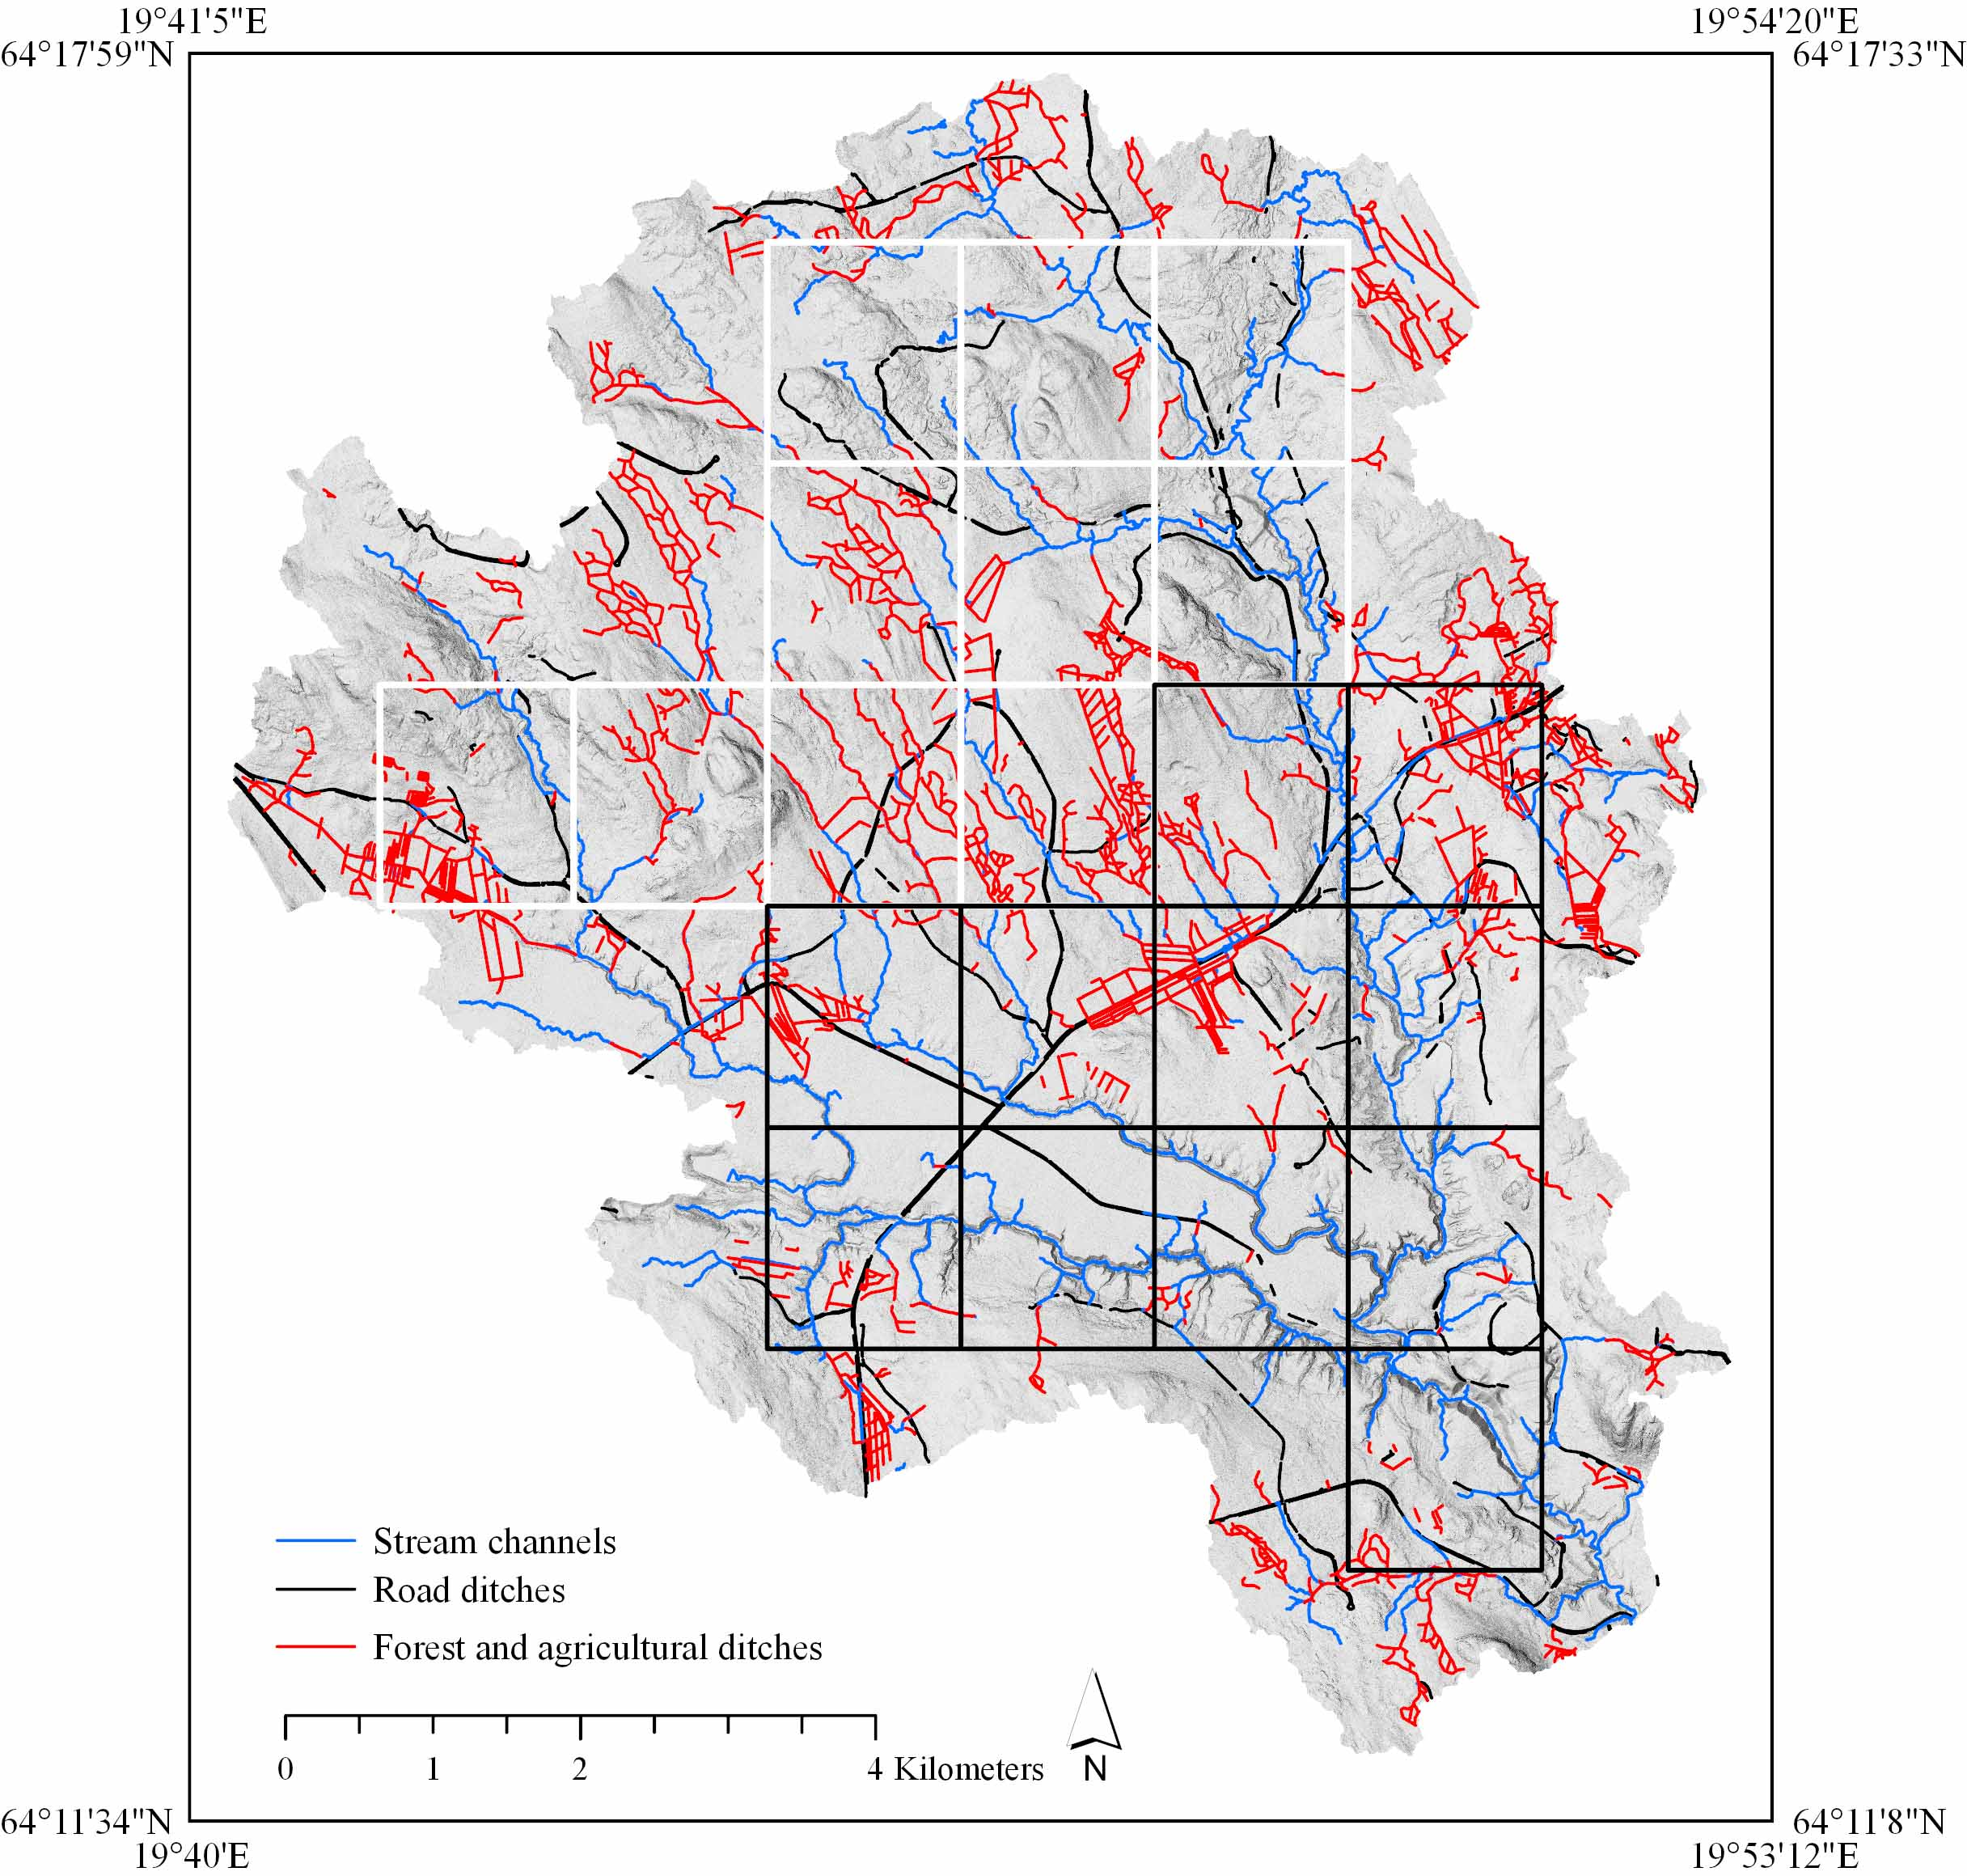
\includegraphics[width=1\linewidth]{./images/Krycklan_lo.jpg}
    \caption{Map of Krycklan showing ditches and stream channels, as well as our division into 21 subsections. The 10 subsections with a white border were used for developing \DIFdelbeginFL \DIFdelFL{the model }\DIFdelendFL \DIFaddbeginFL \DIFaddFL{input variables and optimising parameters }\DIFaddendFL before the experiment. The 11 subsections with a black border were used in the experiment for evaluation with 11-fold cross validation. Each rectangular subsection represents $2997 \cdot 2620$ pixels (roughly 196 hectare).}
    \label{fig:swedenkrycklan}
\end{figure}

From the ditch mapping, the vector layer was rasterised so \DIFaddbegin \DIFadd{that }\DIFaddend it could be compared to the automatically derived ditches from the $0.5*0.5$ m DEM. \DIFdelbegin \DIFdel{Because the  observed average width of ditches is larger than }\DIFdelend \DIFaddbegin \DIFadd{Our field observations have shown that the  width of most ditches within the catchment ranges between }\DIFaddend 0.5 \DIFdelbegin \DIFdel{metres, }\DIFdelend \DIFaddbegin \DIFadd{and 3.5 m. To ensure that the model received all ditch pixels correctly in the training phase, we widened the ditches so that }\DIFaddend all pixels within a radius of three pixels (1.5 metres) of the vectors were labelled as ditch pixels. \hyperref[fig:ditchpreprocess]{Figure} \ref{fig:ditchpreprocess} \hyperref[fig:ditchpreprocess]{a} shows the ditches rasterised from vectors and \hyperref[fig:ditchpreprocess]{Figure} \ref{fig:ditchpreprocess} \hyperref[fig:ditchpreprocess]{b} shows the ditches after widening. The data in \hyperref[fig:ditchpreprocess]{Figure} \ref{fig:ditchpreprocess} \hyperref[fig:ditchpreprocess]{b} is the labelled data that was used to train the \DIFdelbegin \DIFdel{Random Forests model}\DIFdelend \DIFaddbegin \DIFadd{machine learning models}\DIFaddend . The ditches all have a generalised width based on a perceived average of ditch width in the area. Due to all ditches varying in width, it was impossible to produce a perfect representation of each ditch\DIFdelbegin \DIFdel{. However, this made for a good compromise for the average ditch }\DIFdelend \DIFaddbegin \DIFadd{, but this widening helped ensure that almost all ditch pixels were covered by the labels}\DIFaddend .

\DIFdelbegin \DIFdel{Because our priority was to detect ditches, rather than accurately detecting each pixel labelled as a ditch, some adjustments were made when producing the prediction results. The dataset was divided into a lower resolution grid }\DIFdelend \DIFaddbegin \DIFadd{To match the labels with out predictions (where we downscale the predictions into grids to remove outliers), the ground-truth was also downscaled into grids }\DIFaddend of $6*6$ pixels (9 $m^2$) \DIFdelbegin \DIFdel{for eachgrid}\DIFdelend \DIFaddbegin \DIFadd{each}\DIFaddend . Each grid cell that contained at least 25\% ditch pixels was \DIFdelbegin \DIFdel{then }\DIFdelend labelled as a ditch, see \hyperref[fig:ditchpreprocess]{Figure} \ref{fig:ditchpreprocess} \hyperref[fig:ditchpreprocess]{c}. This layer was used to ground-truth the \DIFdelbegin \DIFdel{Random Forests model}\DIFdelend \DIFaddbegin \DIFadd{machine learning models}\DIFaddend .

\begin{figure} [htb!]
    \centering
    \subfigure[]{
        \resizebox*{4.5cm}{!}{\includegraphics{./images/publ_ditch_preprocess_A_lo.jpg}}}\hspace{5pt}
    \subfigure[]{
        \resizebox*{4.5cm}{!}{\includegraphics{./images/publ_ditch_preprocess_B_lo.jpg}}}
    \subfigure[]{
        \resizebox*{4.5cm}{!}{\includegraphics{./images/publ_ditch_preprocess_C_lo.jpg}}}
    \caption{Processing of ditch labels. \textbf{a: }Rasterised ditches with a width of one pixel. \textbf{b: }Ditches after a widening process, seven pixels (3.5 metres) wide. Used as input when training the \DIFdelbeginFL \DIFdelFL{model}\DIFdelendFL \DIFaddbeginFL \DIFaddFL{models}\DIFaddendFL . \textbf{c: }Ditches after a grid zone conversion. Used for evaluating the results from the \DIFdelbeginFL \DIFdelFL{model}\DIFdelendFL \DIFaddbeginFL \DIFaddFL{ditch detector}\DIFaddendFL .} \label{sample-figure}
    \label{fig:ditchpreprocess}
\end{figure}

\subsection{Extracting ditches with digital terrain indices}
From the DEM, several digital terrain indices were calculated\DIFaddbegin \DIFadd{. The strengths and weaknesses of these indices have been obtained from observing their performance in different topological environments}\DIFaddend :
\begin{itemize} \label{data_attributes}

  \item \textbf{Sky View Factor} \newline
    The Sky View Factor \DIFdelbegin \DIFdel{is a digital terrain index with a value ranging from 0 to 1, representing }\DIFdelend \DIFaddbegin \DIFadd{represents }\DIFaddend how much of the sky that is visible from a certain point on the ground \citep{zaksek}. \DIFdelbegin \DIFdel{On an open field all of the sky would be visible, but at the bottom of a ditch much of the sky would be obscured , meaning low values would indicate ditches. This method tends to give }\DIFdelend \DIFaddbegin \DIFadd{A point in a ditch would yield a low value, as more of the sky is obscured by the ditch bank. However, it tends to produce }\DIFaddend false positives in steep terrain\DIFdelbegin \DIFdel{, where the sky can be obscured by a hillside, or in narrow valleys or ravines that also show low numbers}\DIFdelend . The Sky View Factor was calculated in SAGA GIS, using a search radius of 10 \DIFdelbegin \DIFdel{m}\DIFdelend \DIFaddbegin \DIFadd{metres to ensure that it was large enough to capture the ditches, but small enough to not include large scale topographical features such as hills}\DIFaddend .

  \item \textbf{Impoundment Index}\newline
    The \DIFdelbegin \DIFdel{tool }\DIFdelend Impoundment Index in Whitebox Tools \citep{whiteboxtools} \DIFdelbegin \DIFdel{is a digital terrain index designed to serve }\DIFdelend \DIFaddbegin \DIFadd{can be used }\DIFaddend as a measure of \DIFdelbegin \DIFdel{topographic incision and flow constriction. The index }\DIFdelend \DIFaddbegin \DIFadd{flow constriction, which is useful for mapping channels, such as ditches. When tuned to output the flooded volume, it }\DIFaddend effectively maps the area and average depth of the reservoir that would be created by placing a dam of a user-specified length at each grid cell in the DEM. \DIFdelbegin \DIFdel{The tool can be tuned to output the flooded area or volume (in which case it highlights areas of flow constriction), or the average flooded depth (which seems to measure topographic incision). Additionally, the tool will output a 'dam height' raster that is particularly useful for mapping channels, such as ditches. }\DIFdelend Here, we used dam height calculated with a dam length of 3 \DIFdelbegin \DIFdel{m}\DIFdelend \DIFaddbegin \DIFadd{metres to cover the entire ditches}\DIFaddend . Typical false positives with this method are natural stream channels with a clear incised channel.

  \item \textbf{High Pass Median Filter} \newline
    High Pass Median Filters (HPMF) highlight ditches by indicating local depressions \DIFaddbegin \DIFadd{(such as ditches) }\DIFaddend in the DEM \DIFdelbegin \DIFdel{. The algorithm operates essentially }\DIFdelend by subtracting the value at the grid cell at the centre of the window from the median value in the window. \DIFdelbegin \DIFdel{Negative values indicate depressions in the DEM, such as ditches. A typical false positive }\DIFdelend \DIFaddbegin \DIFadd{Typical false positives }\DIFaddend with this index are small hollows\DIFdelbegin \DIFdel{that also show negative numbers}\DIFdelend . HPMF was calculated using Whitebox Tools \citep{whiteboxtools} with a window size of $4.5 * 4.5$ m. 

    \item \textbf{Slope} \newline
    The Slope index represents the degree of slope at a certain point, with a value ranging from $0^{\circ}$ to $90^{\circ}$. It was calculated on the 0.5 m grid, using \DIFdelbegin \DIFdel{ArgGIS }\DIFdelend \DIFaddbegin \DIFadd{ArcGIS }\DIFaddend \citep{EsriArcGisBook}. This index contains no information about the direction of the slope.
\end{itemize}

\subsubsection{Thresholding the digital terrain indices}
To benchmark our method against a non-machine learning method, we binarised the original four digital terrain indices using thresholds. Different threshold values were tested and the value that yielded the highest Cohen's Kappa score for each respective index was chosen. This test was conducted for the 11 subsections described in \ref{trainingvalidationdatasets}. The Sky View Factor index was classified to only include values below 0.955, the Impoundment Index Dam Height using values above 0.27 $m$, the HPMF index using values below -0.18 m, and the Slope index using values above $14 ^{\circ}$ (Table 2). 

\subsection{Data preparation}

\subsubsection{Processing the digital terrain indices}
\DIFdelbegin \DIFdel{Developing the Random Forests model involved examining how different  kinds of }\DIFdelend \DIFaddbegin \DIFadd{We examined how different  }\DIFaddend input variables affected the prediction \DIFaddbegin \DIFadd{of the machine learning models}\DIFaddend . Several possible data manipulation methods could theoretically produce a better prediction. To improve the prediction, steps were taken where neighbouring pixels were included to give a representation of the area surrounding a specific pixel, similar to the approach of \citet{roelens}. 

The digital terrain indices provided a satisfactory foundation for the \DIFdelbegin \DIFdel{model}\DIFdelend \DIFaddbegin \DIFadd{models}\DIFaddend , but lacked in the generalisability of their predictions. More diverse input variables were extracted using simple statistical aggregates such as mean, median, min, max, and standard deviation. \DIFdelbegin \DIFdel{This facilitated finding obscurities in the }\DIFdelend \DIFaddbegin \DIFadd{Using these statistical aggregations with the help of }\DIFaddend neighbouring areas around pixels \DIFaddbegin \DIFadd{aided in pruning pixels with outlier values, often smoothing out the data to represent ditches more accurately on a per-pixel basis}\DIFaddend . These variables were calculated by gathering all data points in different circular radii around the studied pixel, before computing one of the statistical aggregations \DIFdelbegin \DIFdel{, see }\DIFdelend \DIFaddbegin \DIFadd{(}\DIFaddend \hyperref[fig:features]{Figure} \ref{fig:features}: \hyperref[fig:features]{b}, \hyperref[fig:features]{c}, \DIFdelbegin %DIFDELCMD < \hyperref[fig:features]{h}%%%
\DIFdel{, and }%DIFDELCMD < \hyperref[fig:features]{j}%%%
\DIFdelend \DIFaddbegin \hyperref[fig:features]{f}\DIFadd{, and }\hyperref[fig:features]{g}\DIFadd{)}\DIFaddend .

In addition to the general input variables, a number of custom input variables were also developed.  \DIFdelbegin \DIFdel{Several of these variables were calculated by looking at the separate digital terrain indices, attempting to amplify the ditches. This was done in several different ways for the indices by combining statistical aggregations, and }\DIFdelend \DIFaddbegin \DIFadd{Some of these custom variables were produced by statistical aggregation of multiple indices, whereas in some cases, they were generated }\DIFaddend by using thresholds to exclude, lower, or amplify the values of pixels that indicated ditches or non-ditches \DIFdelbegin \DIFdel{, see }\DIFdelend \DIFaddbegin \DIFadd{(}\DIFaddend \hyperref[fig:features]{Figure} \ref{fig:features}: \DIFdelbegin %DIFDELCMD < \hyperref[fig:features]{e} %%%
\DIFdel{and }%DIFDELCMD < \hyperref[fig:features]{k}%%%
\DIFdelend \DIFaddbegin \hyperref[fig:features]{d} \DIFadd{and }\hyperref[fig:features]{h}\DIFadd{)}\DIFaddend .

\DIFdelbegin \DIFdel{From the Slope and Sky View Factor indices, input variables for the model were also extracted to attempt to amplify the values of pixels that lay in streams or in hilly areas, but leave pixels in ditches or other geographical areas untouched, see }%DIFDELCMD < \hyperref[fig:features]{Figure} %%%
\DIFdel{\ref{fig:features}: }%DIFDELCMD < \hyperref[fig:features]{i}%%%
\DIFdel{.
}%DIFDELCMD < 

%DIFDELCMD < \label{skyviewconic}
%DIFDELCMD < %%%
\DIFdel{The }\textit{\DIFdel{Sky View Factor Conic filter}} %DIFAUXCMD
\DIFdel{was developed to attempt to detect and fill gaps in ditches. This was done by calculating the mean of all the pixels covered by a cone-shaped mask with a radius of 5 metres, which expanded outwards from the examined pixel point in eight directions. If two opposing mean values were both below a threshold, the pixel was given a lower value. This meant that only pixels with strong ditch indicative values in two opposing directions were updated, allowing the filter to avoid updating pixels in cavities or hollows, focusing only on linear geographical properties.
}%DIFDELCMD < 

%DIFDELCMD < \newpage
%DIFDELCMD < 

%DIFDELCMD < %%%
\DIFdelend Both HPMF and Sky View Factor were used with the image processing \textit{gabor filter}, which can be used to detect lines of a certain orientation in an image \citep{gabor}. \DIFdelbegin \DIFdel{To detect lines in all directions, }\DIFdelend 30 Gabor filters \DIFdelbegin \DIFdel{, }\DIFdelend which were rotated in different angles and with different frequencies \DIFdelbegin \DIFdel{, }\DIFdelend were combined to \DIFdelbegin \DIFdel{amplify ditches, see }\DIFdelend \DIFaddbegin \DIFadd{detect lines, amplifying ditches by utilising the fact that ditches have a linear elongated shape (}\DIFaddend \hyperref[fig:features]{Figure} \ref{fig:features}: \DIFdelbegin %DIFDELCMD < \hyperref[fig:features]{d} %%%
\DIFdel{and }%DIFDELCMD < \hyperref[fig:features]{g}%%%
\DIFdelend \DIFaddbegin \hyperref[fig:features]{e}\DIFadd{)}\DIFaddend .

\label{impoundmentstreamremoval}
The raw Impoundment Index dam height was used to create a mask, attempting to \DIFdelbegin \DIFdel{mark }\DIFdelend \DIFaddbegin \DIFadd{mask }\DIFaddend out streams, but retain ditches. Only areas with a relatively high \DIFdelbegin \DIFdel{dam height, above 14 metres, }\DIFdelend \DIFaddbegin \DIFadd{value, }\DIFaddend which would indicate that these areas most likely contained streams, were \DIFdelbegin \DIFdel{marked }\DIFdelend \DIFaddbegin \DIFadd{masked }\DIFaddend out. After widening the resulting area, this mask was used to \DIFdelbegin \DIFdel{attempt to }\DIFdelend remove streams from all the aforementioned custom input variables, generating one new input variable from each. The features marked with \textit{streams removed} in \hyperref[featuretable]{Table} \ref{featuretable} make use of this filter (\hyperref[fig:features]{Figure} \ref{fig:features}\DIFdelbegin %DIFDELCMD < \hyperref[fig:features]{f} %%%
\DIFdel{and }%DIFDELCMD < \hyperref[fig:features]{l}%%%
\DIFdel{).
}\DIFdelend \DIFaddbegin \DIFadd{: }\hyperref[fig:features]{i}\DIFadd{).
}\DIFaddend 

\DIFaddbegin \DIFadd{Overall, 81 input variables were extracted from the terrain indices. In a pilot study, we compared several different algorithms (Random Forests, Extreme Gradient Boosting, Naive Bayes, and Support Vector Machines), and it was found that Random Forests produced the most accurate results, here we therefore only present the results from the Random Forest model. We then conducted a sub-experiment to find the best input variables, as well as the optimal number of variables to use. The variable importance score in Random Forests was used to select the most important input variables and it was found that using the top 40 input variables produced the best results.
}

\DIFaddend \begin{figure} [!htb]
    \centering
    \subfigure[]{
        \resizebox*{4cm}{!}{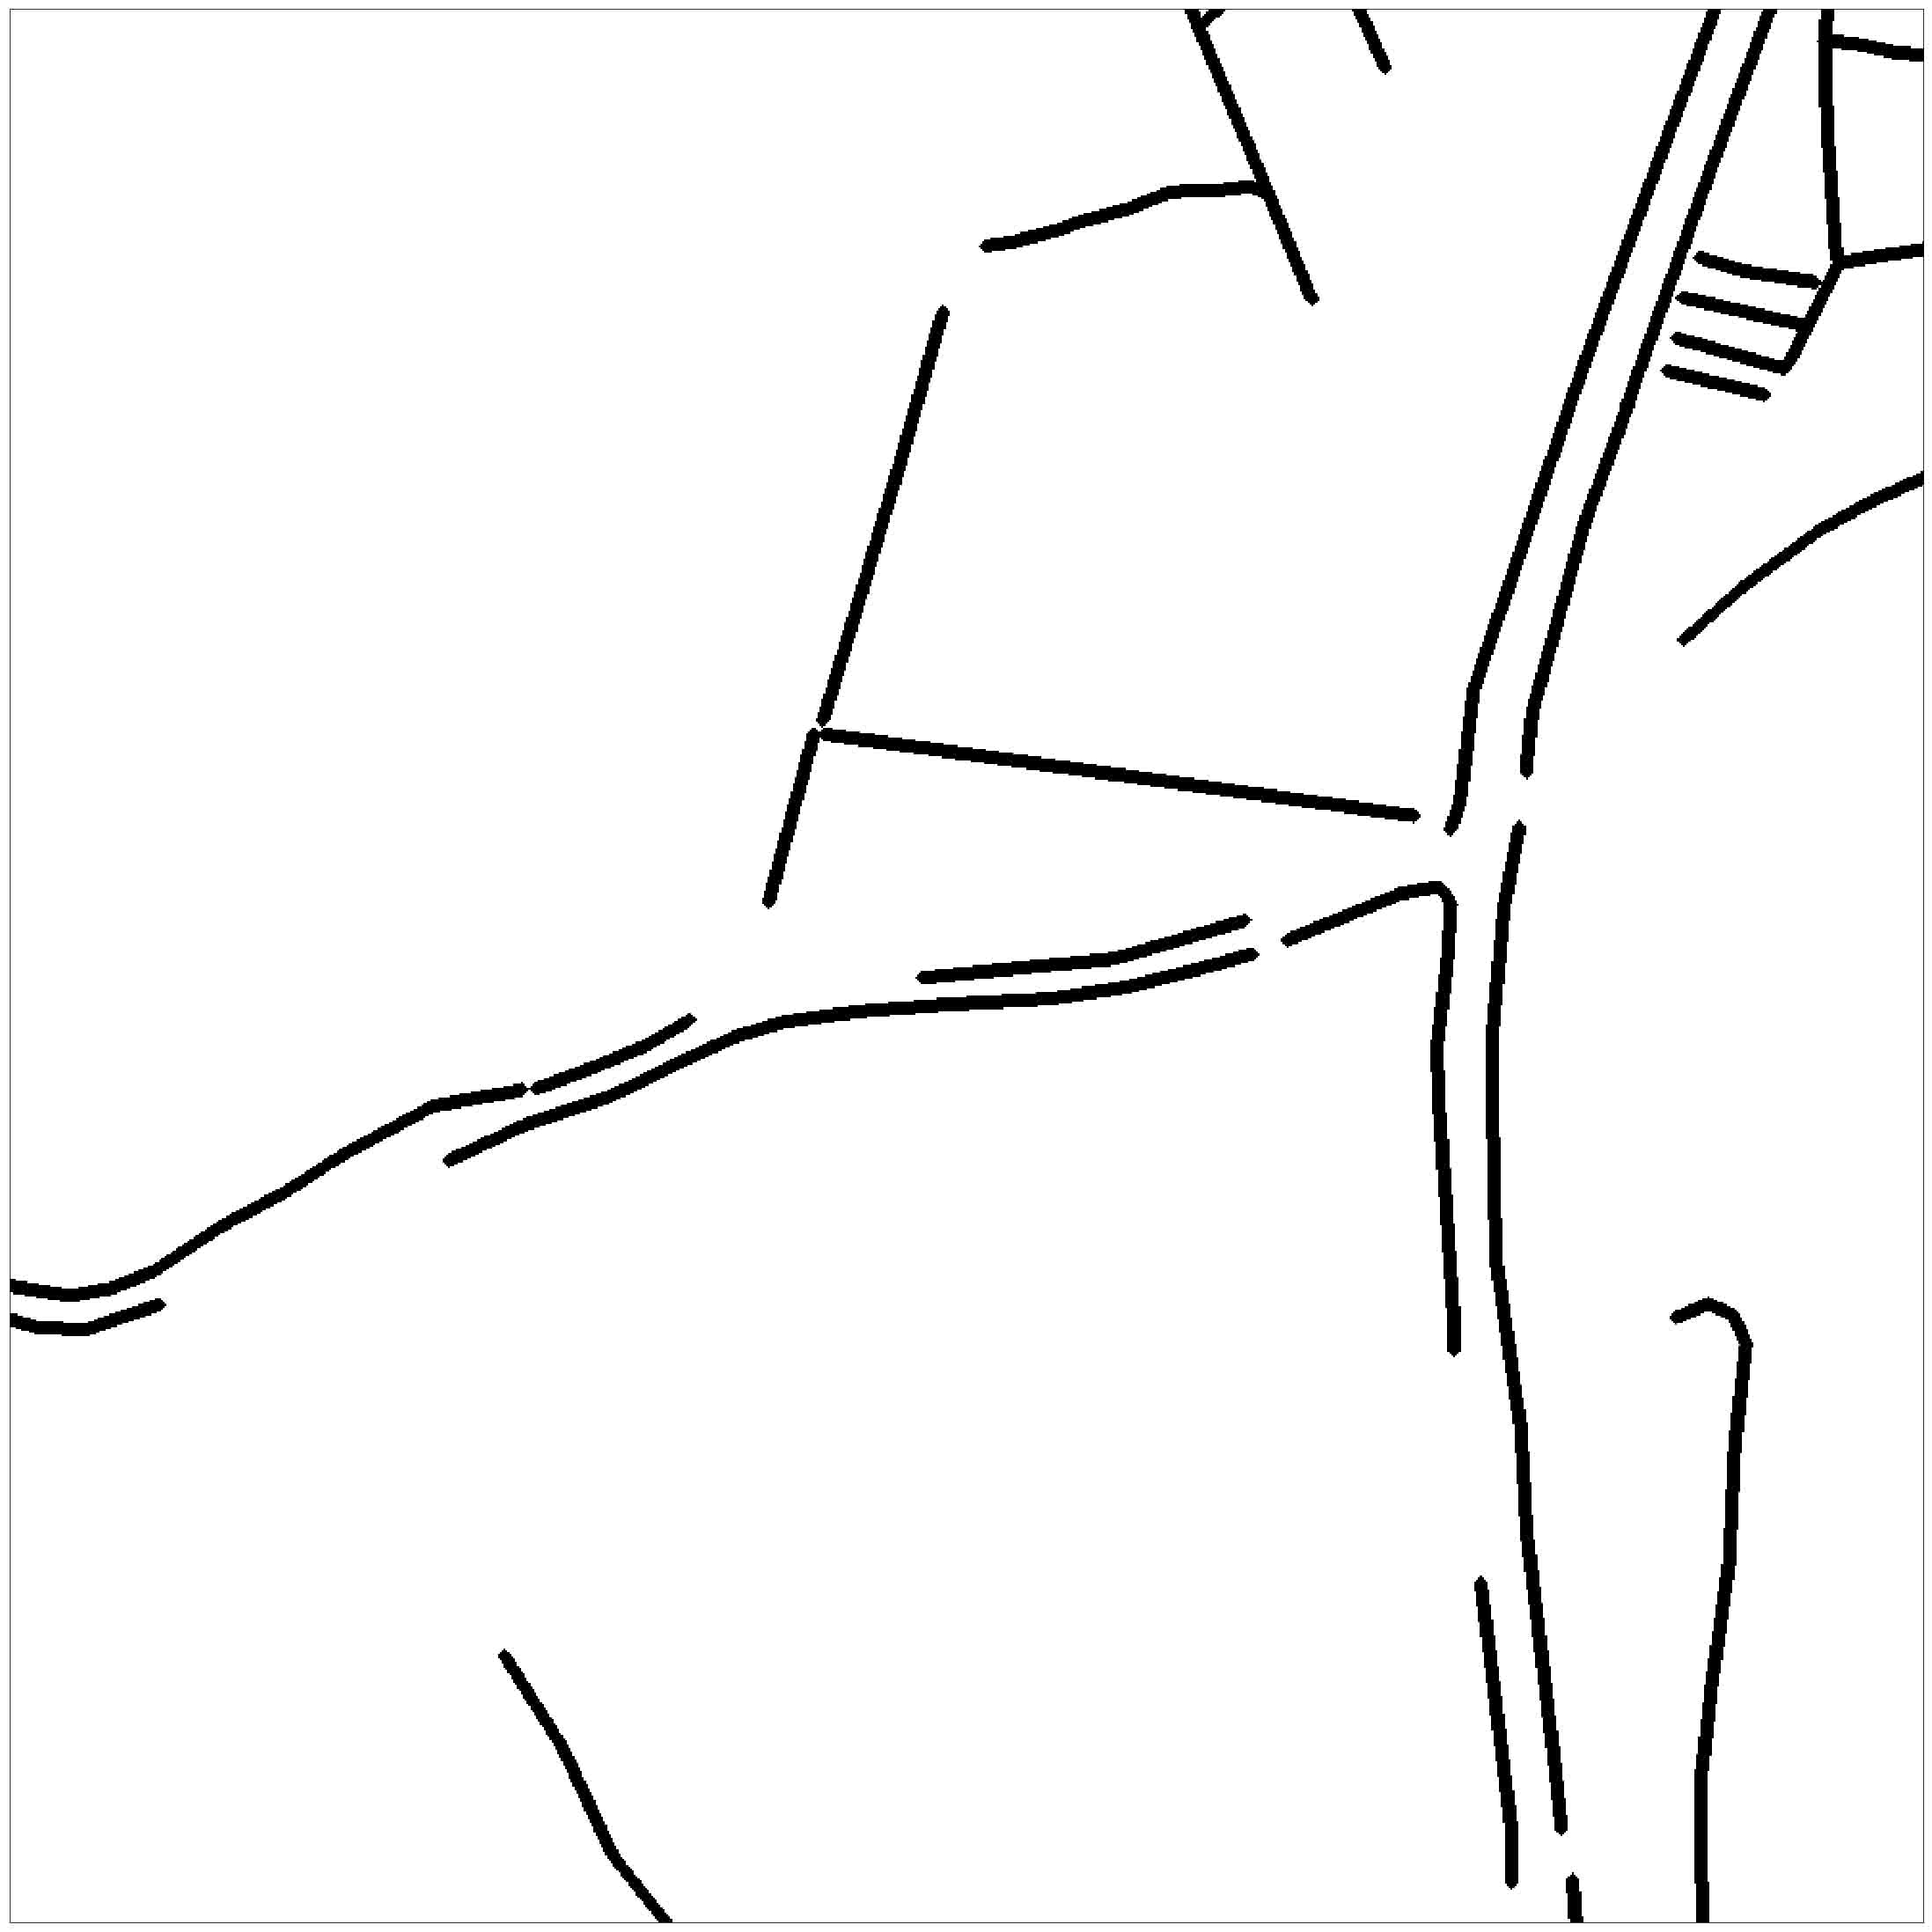
\includegraphics{./images/feature_a_lo.jpg}}}\hspace{5pt}
    \subfigure[]{
        \resizebox*{4cm}{!}{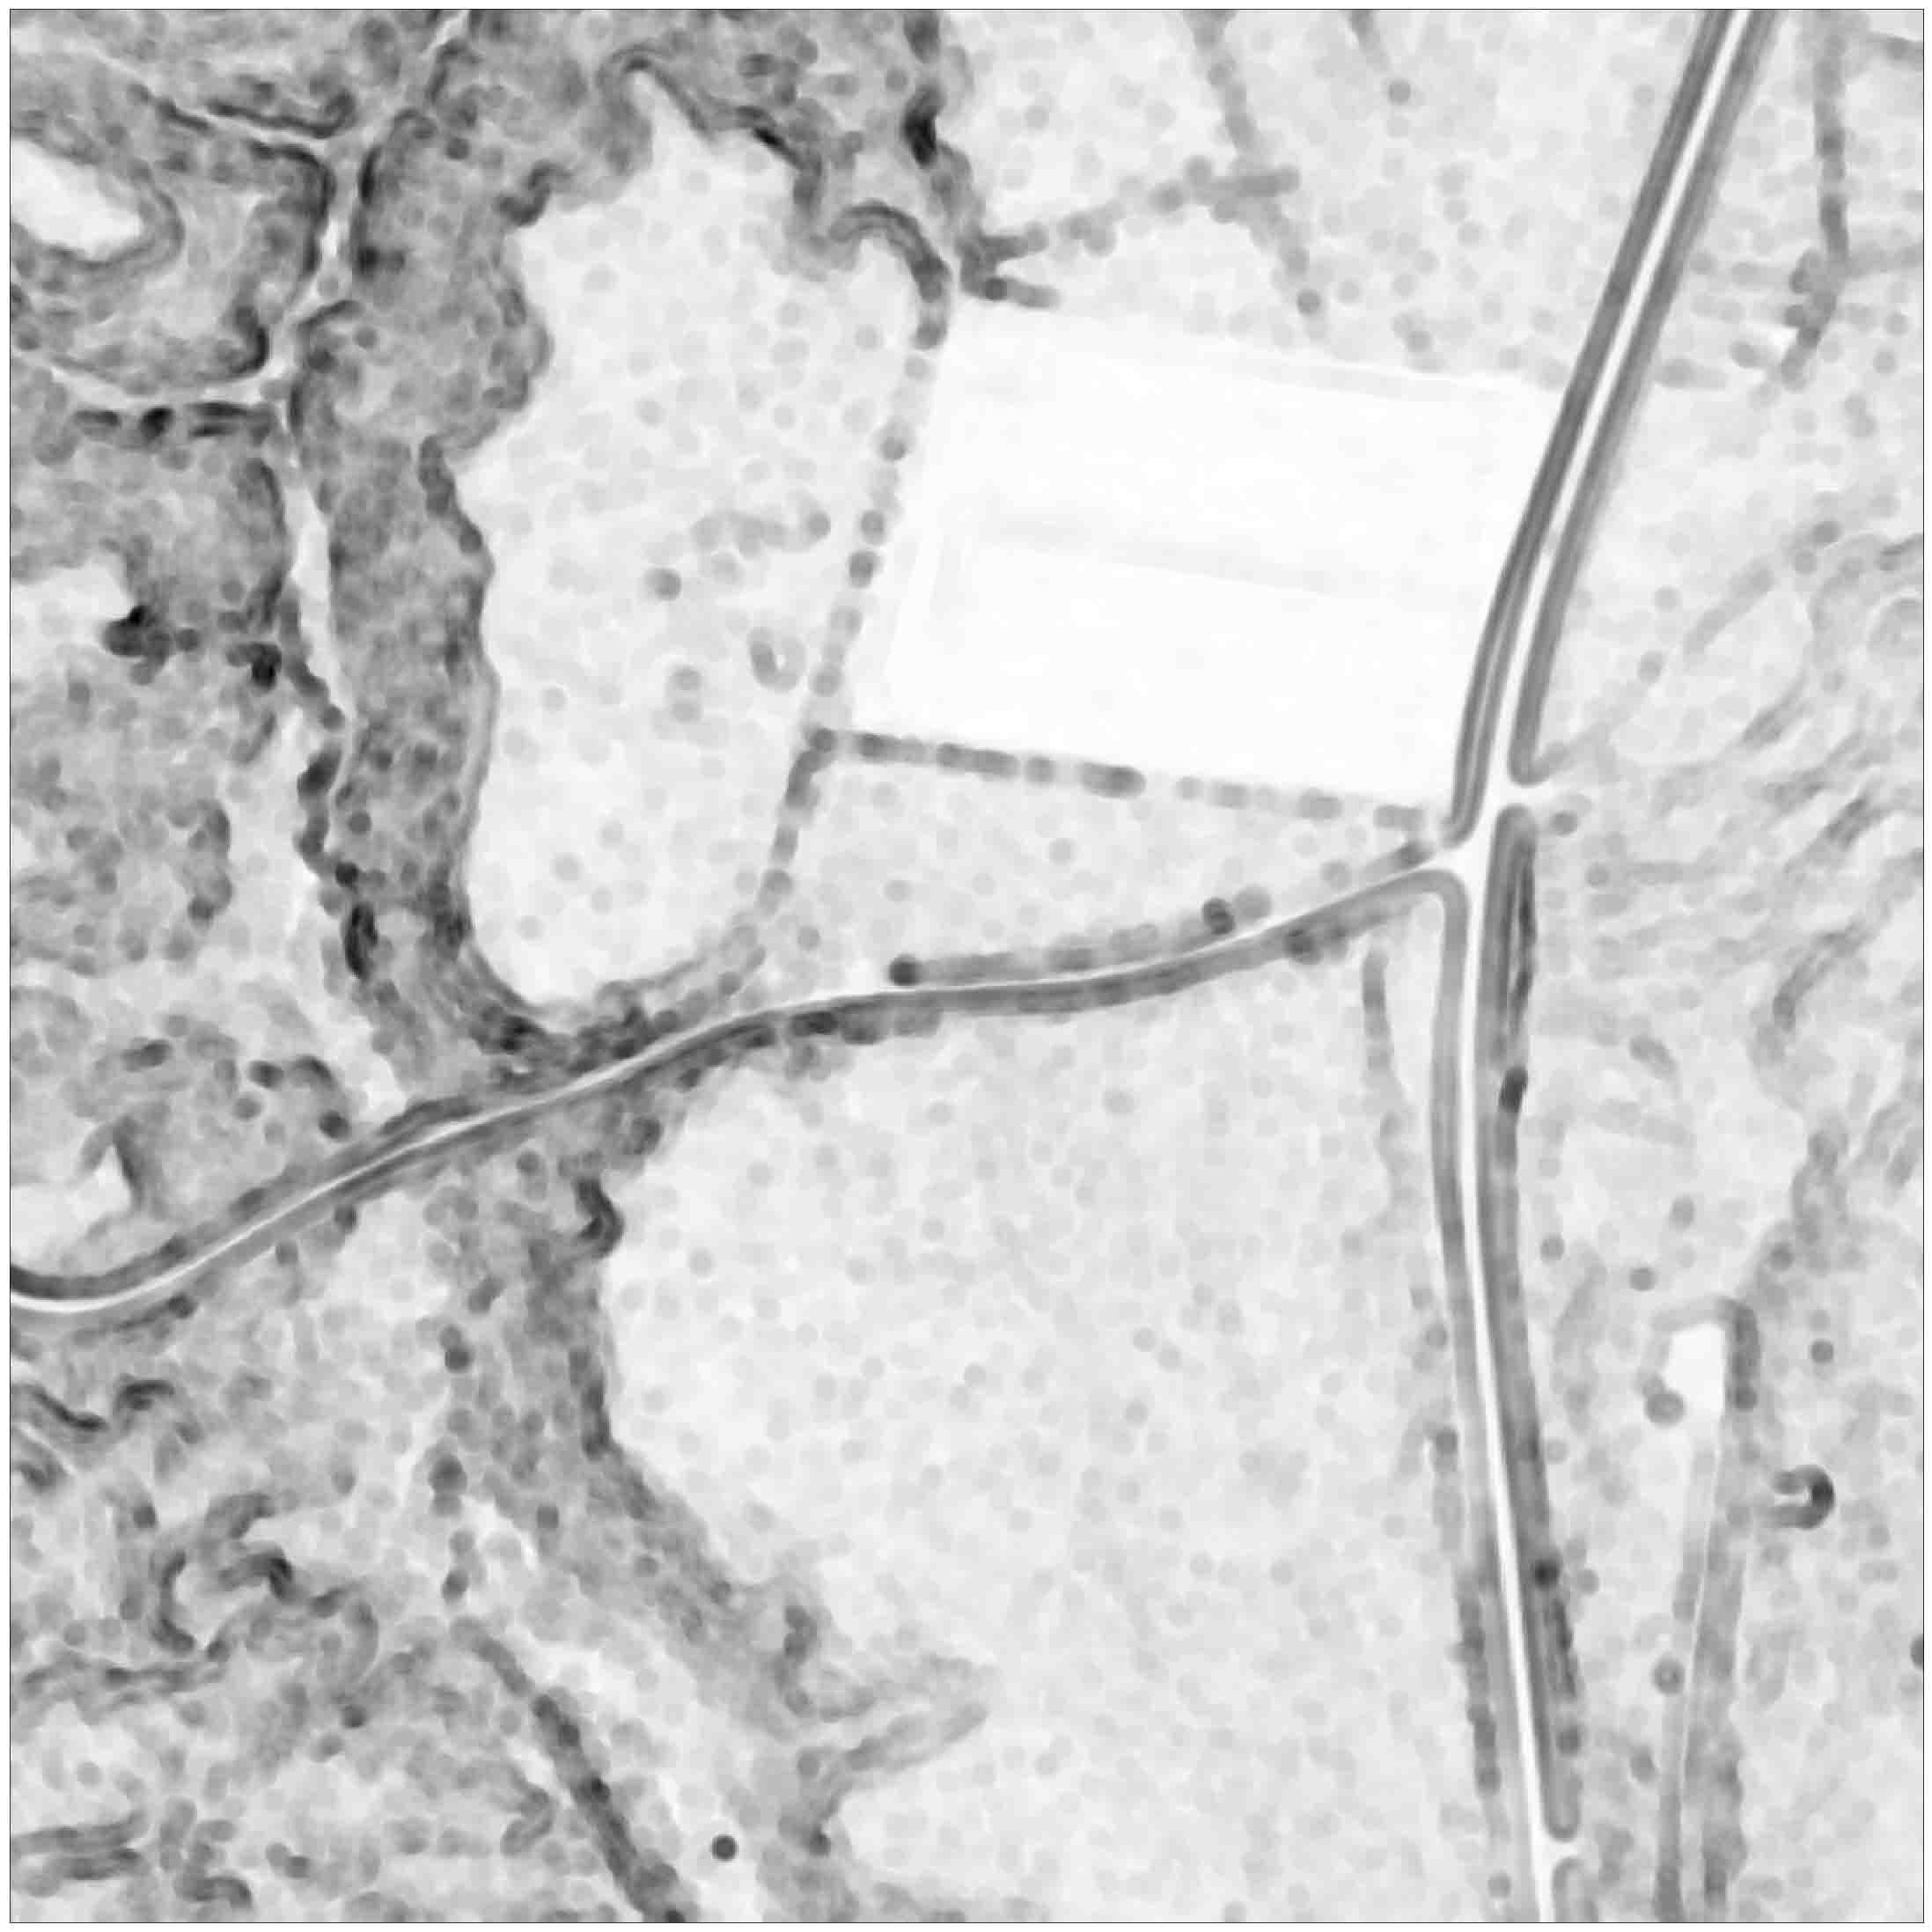
\includegraphics{./images/feature_b_lo.jpg}}}
    \subfigure[]{
        \resizebox*{4cm}{!}{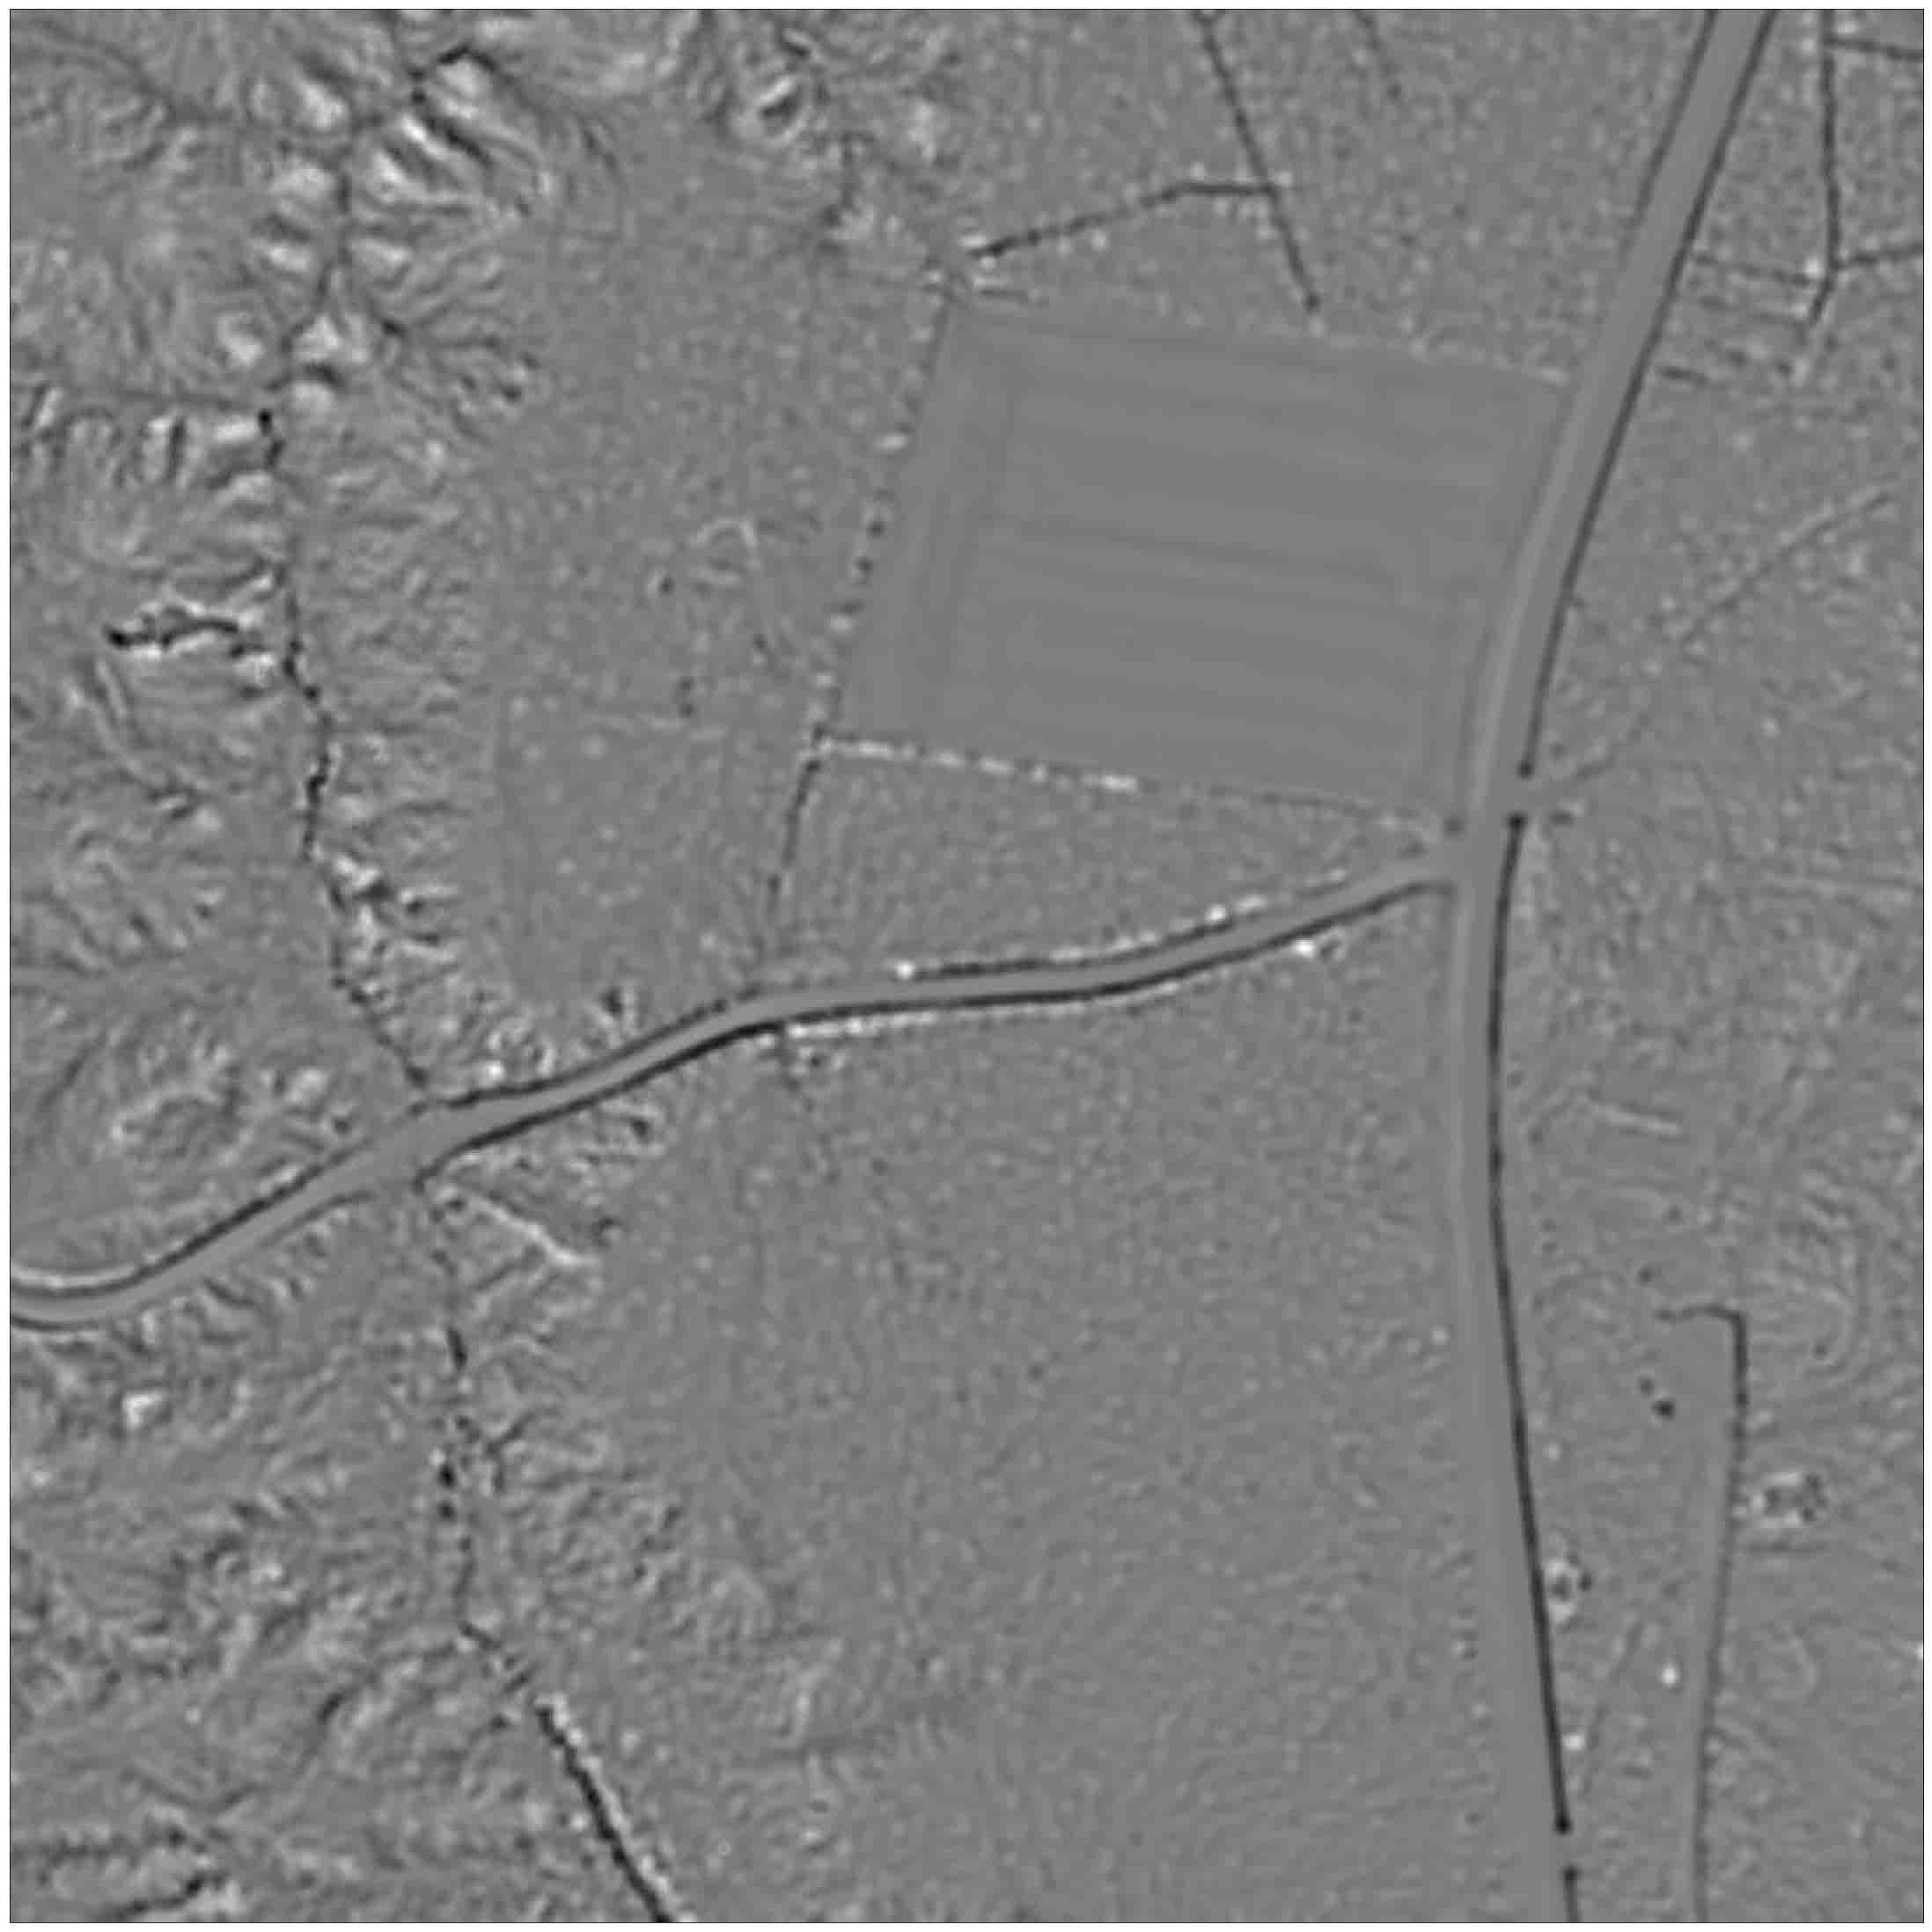
\includegraphics{./images/feature_c_lo.jpg}}}\hspace{5pt}
    \subfigure[]{
        \resizebox*{4cm}{!}{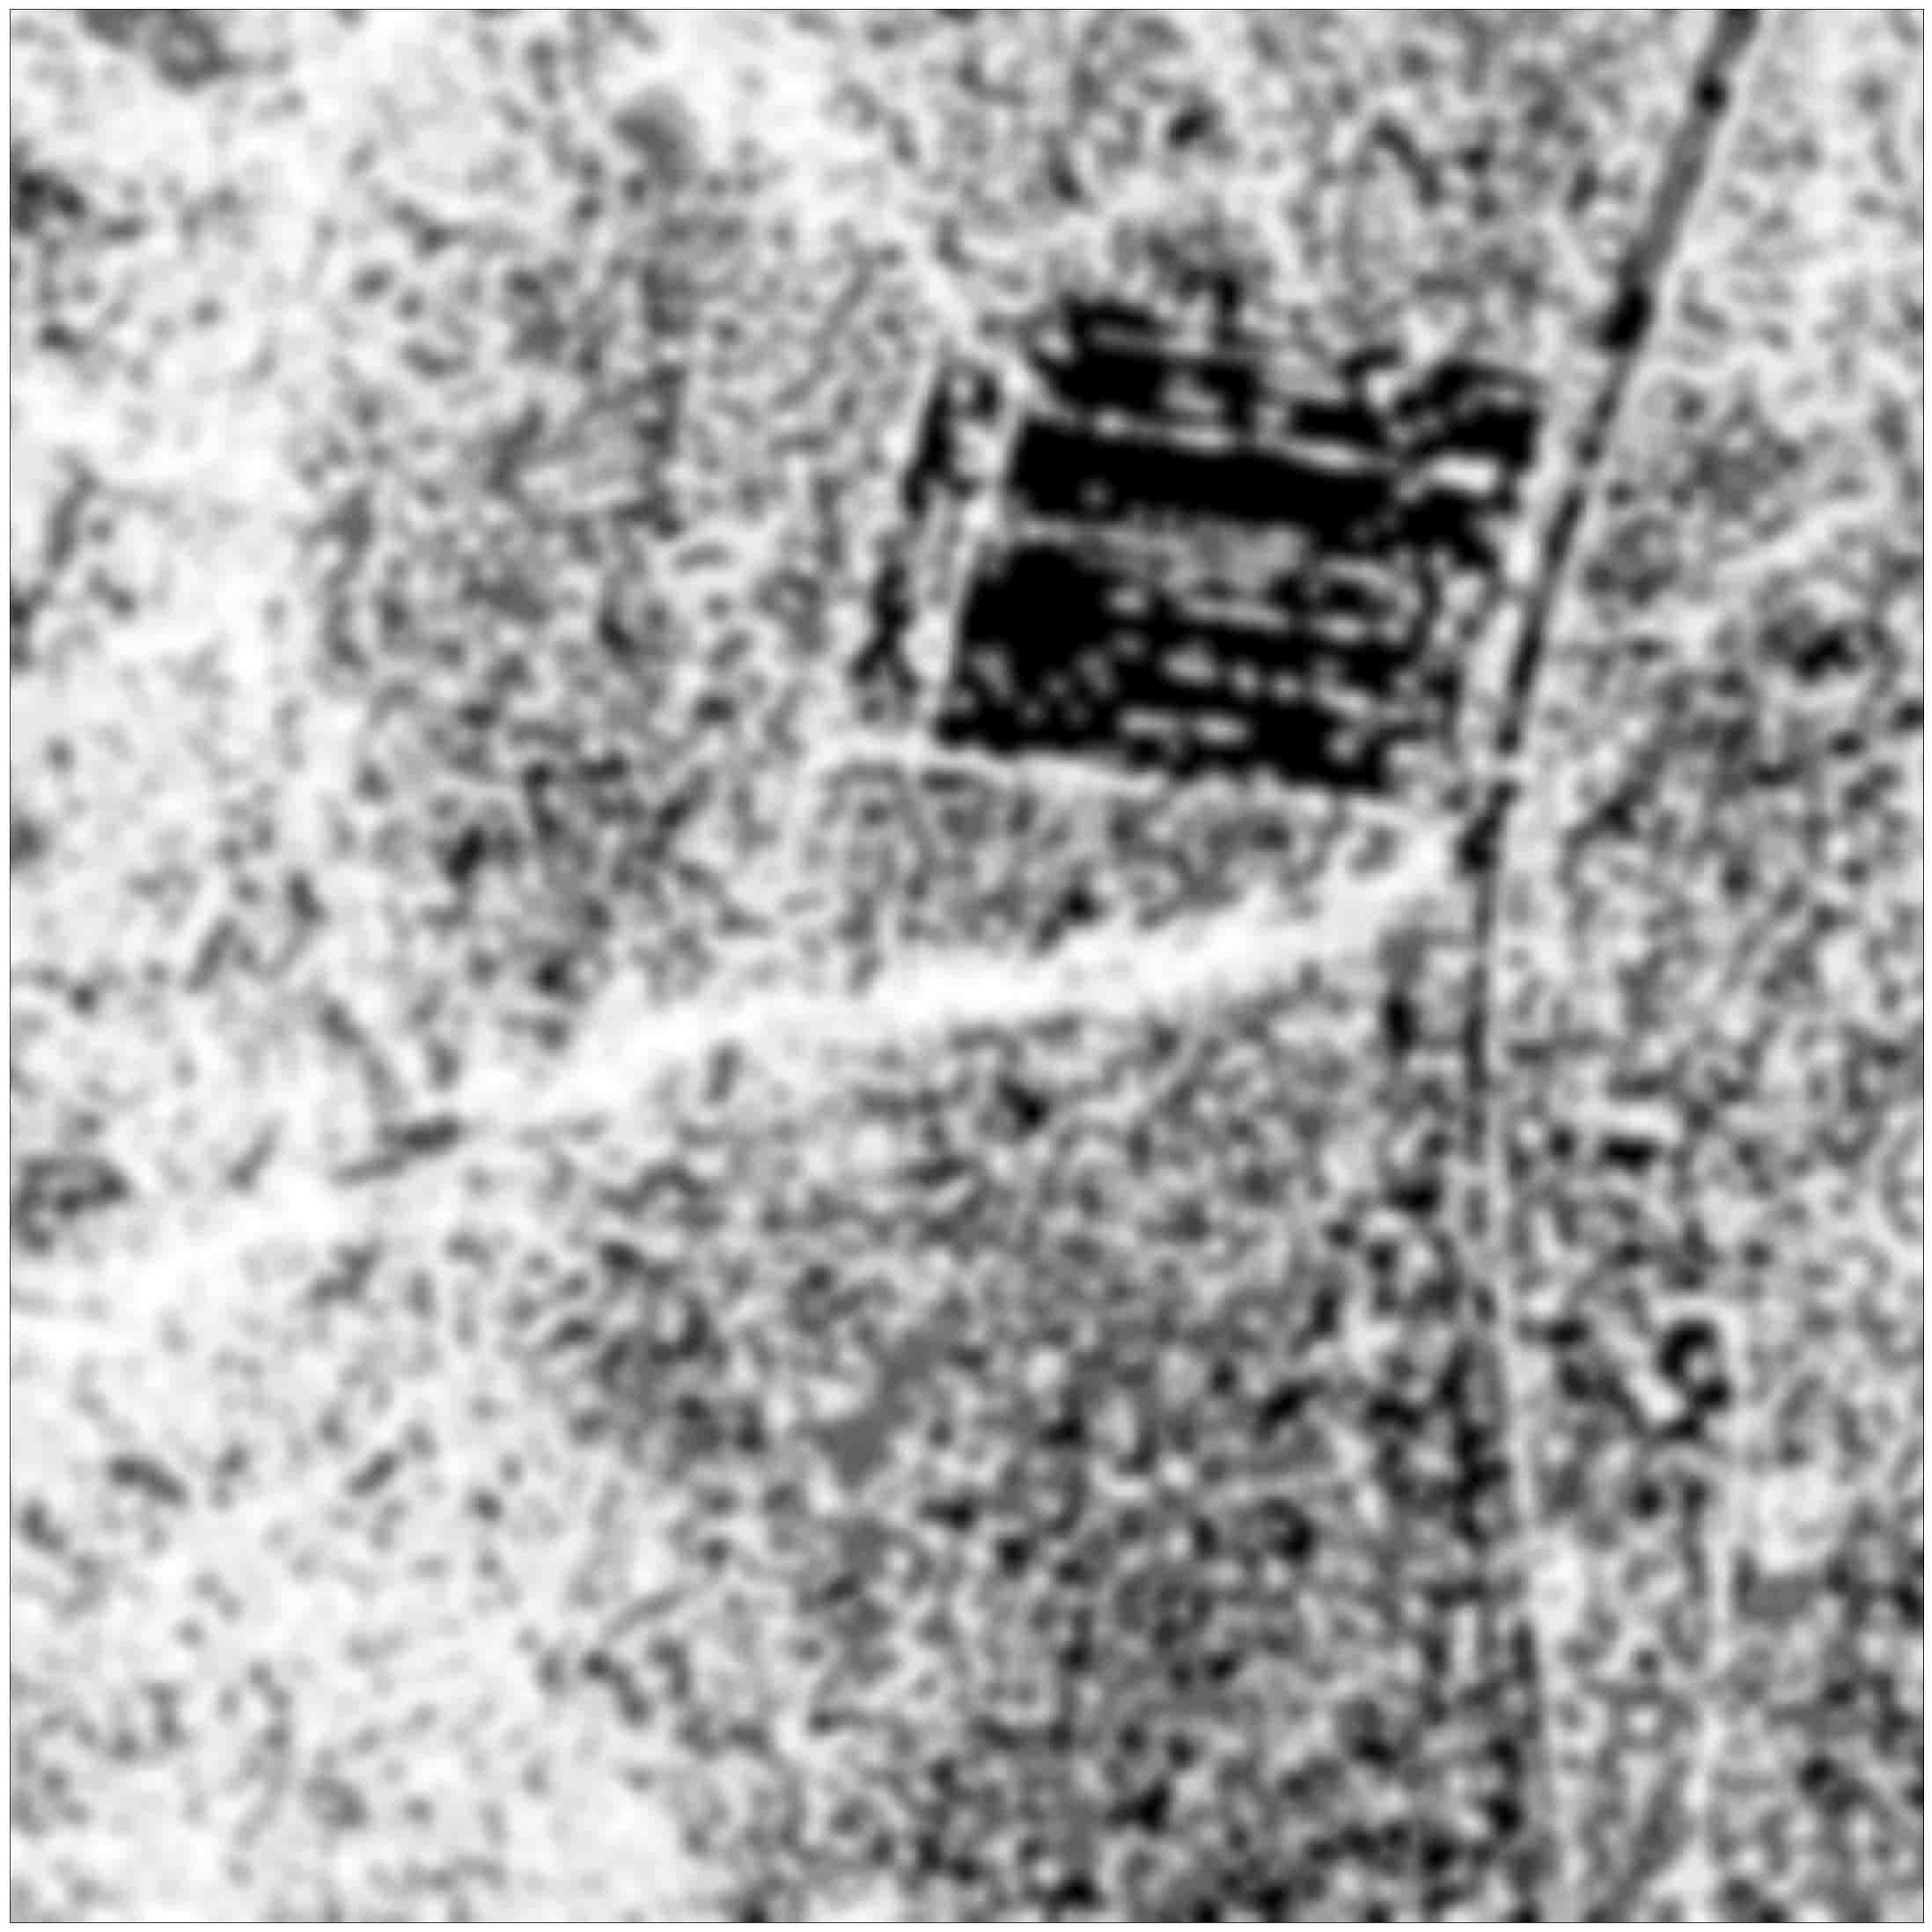
\includegraphics{./images/feature_d_lo.jpg}}}
    \DIFdelbeginFL \DIFdelFL{\hspace{5pt}
    }\DIFdelendFL \subfigure[]{
        \resizebox*{4cm}{!}{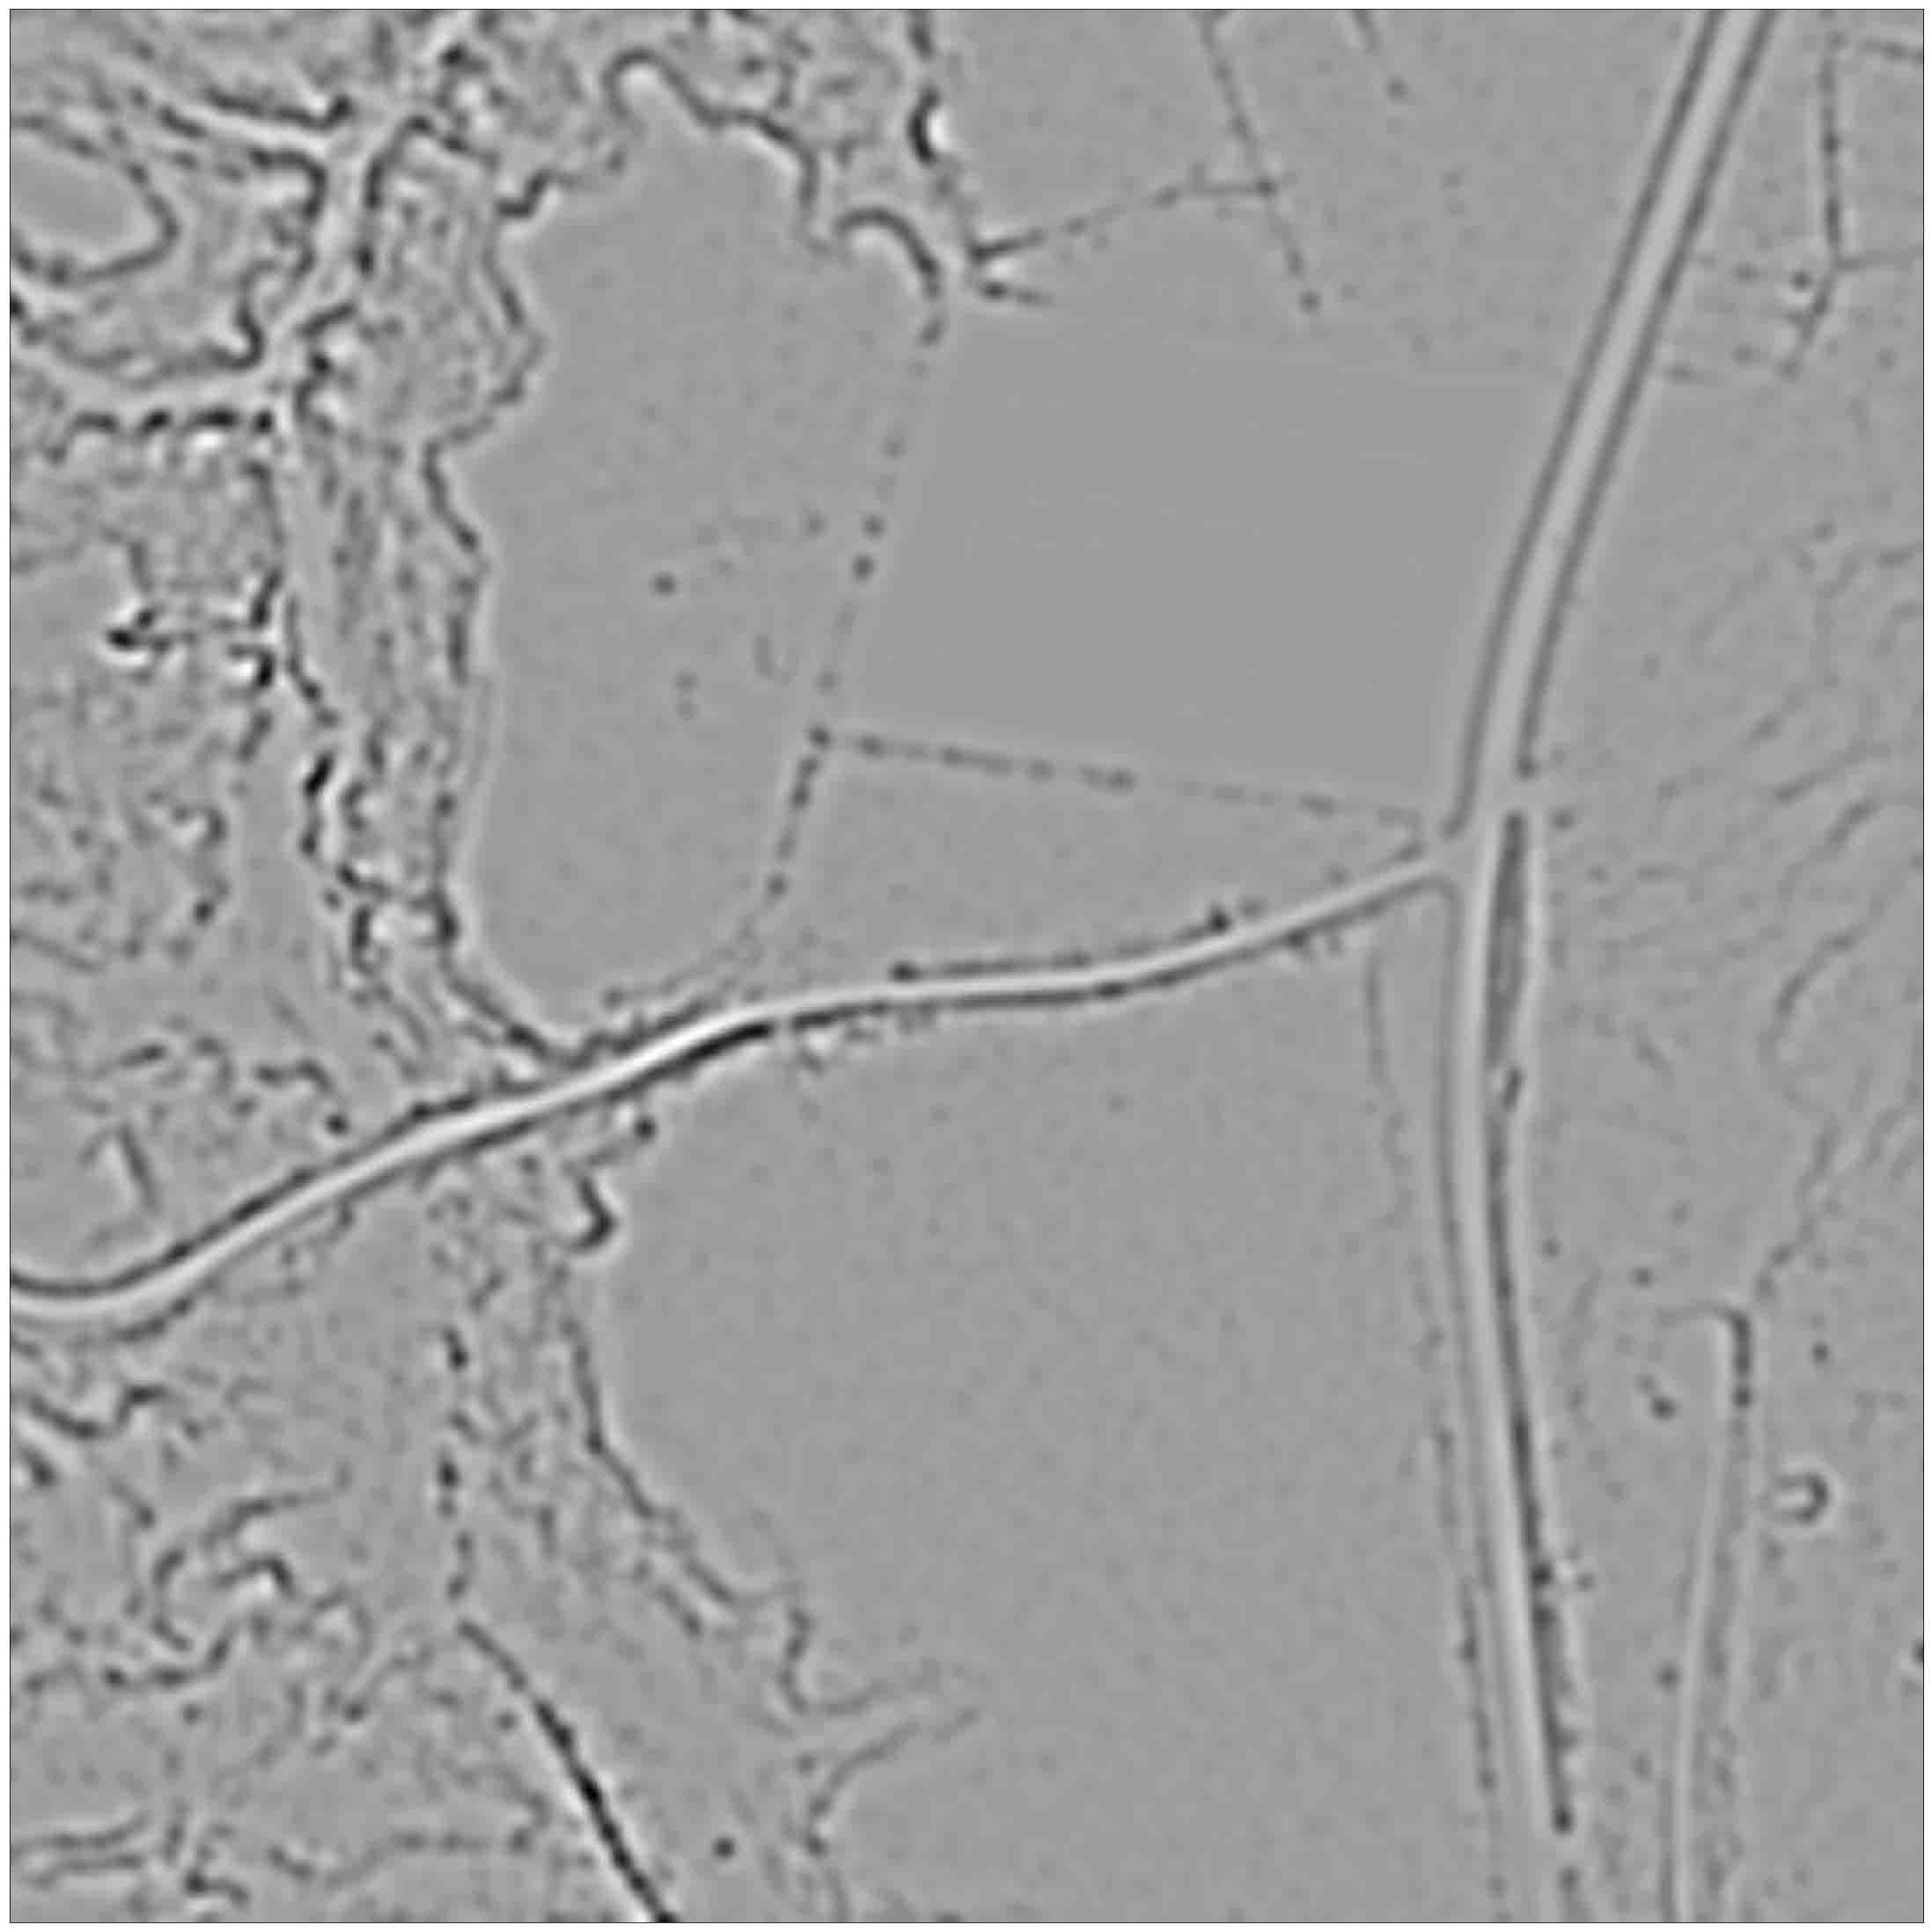
\includegraphics{./images/feature_e_lo.jpg}}}\DIFdelbeginFL %DIFDELCMD < \subfigure[]{
%DIFDELCMD <         \resizebox*{4cm}{!}{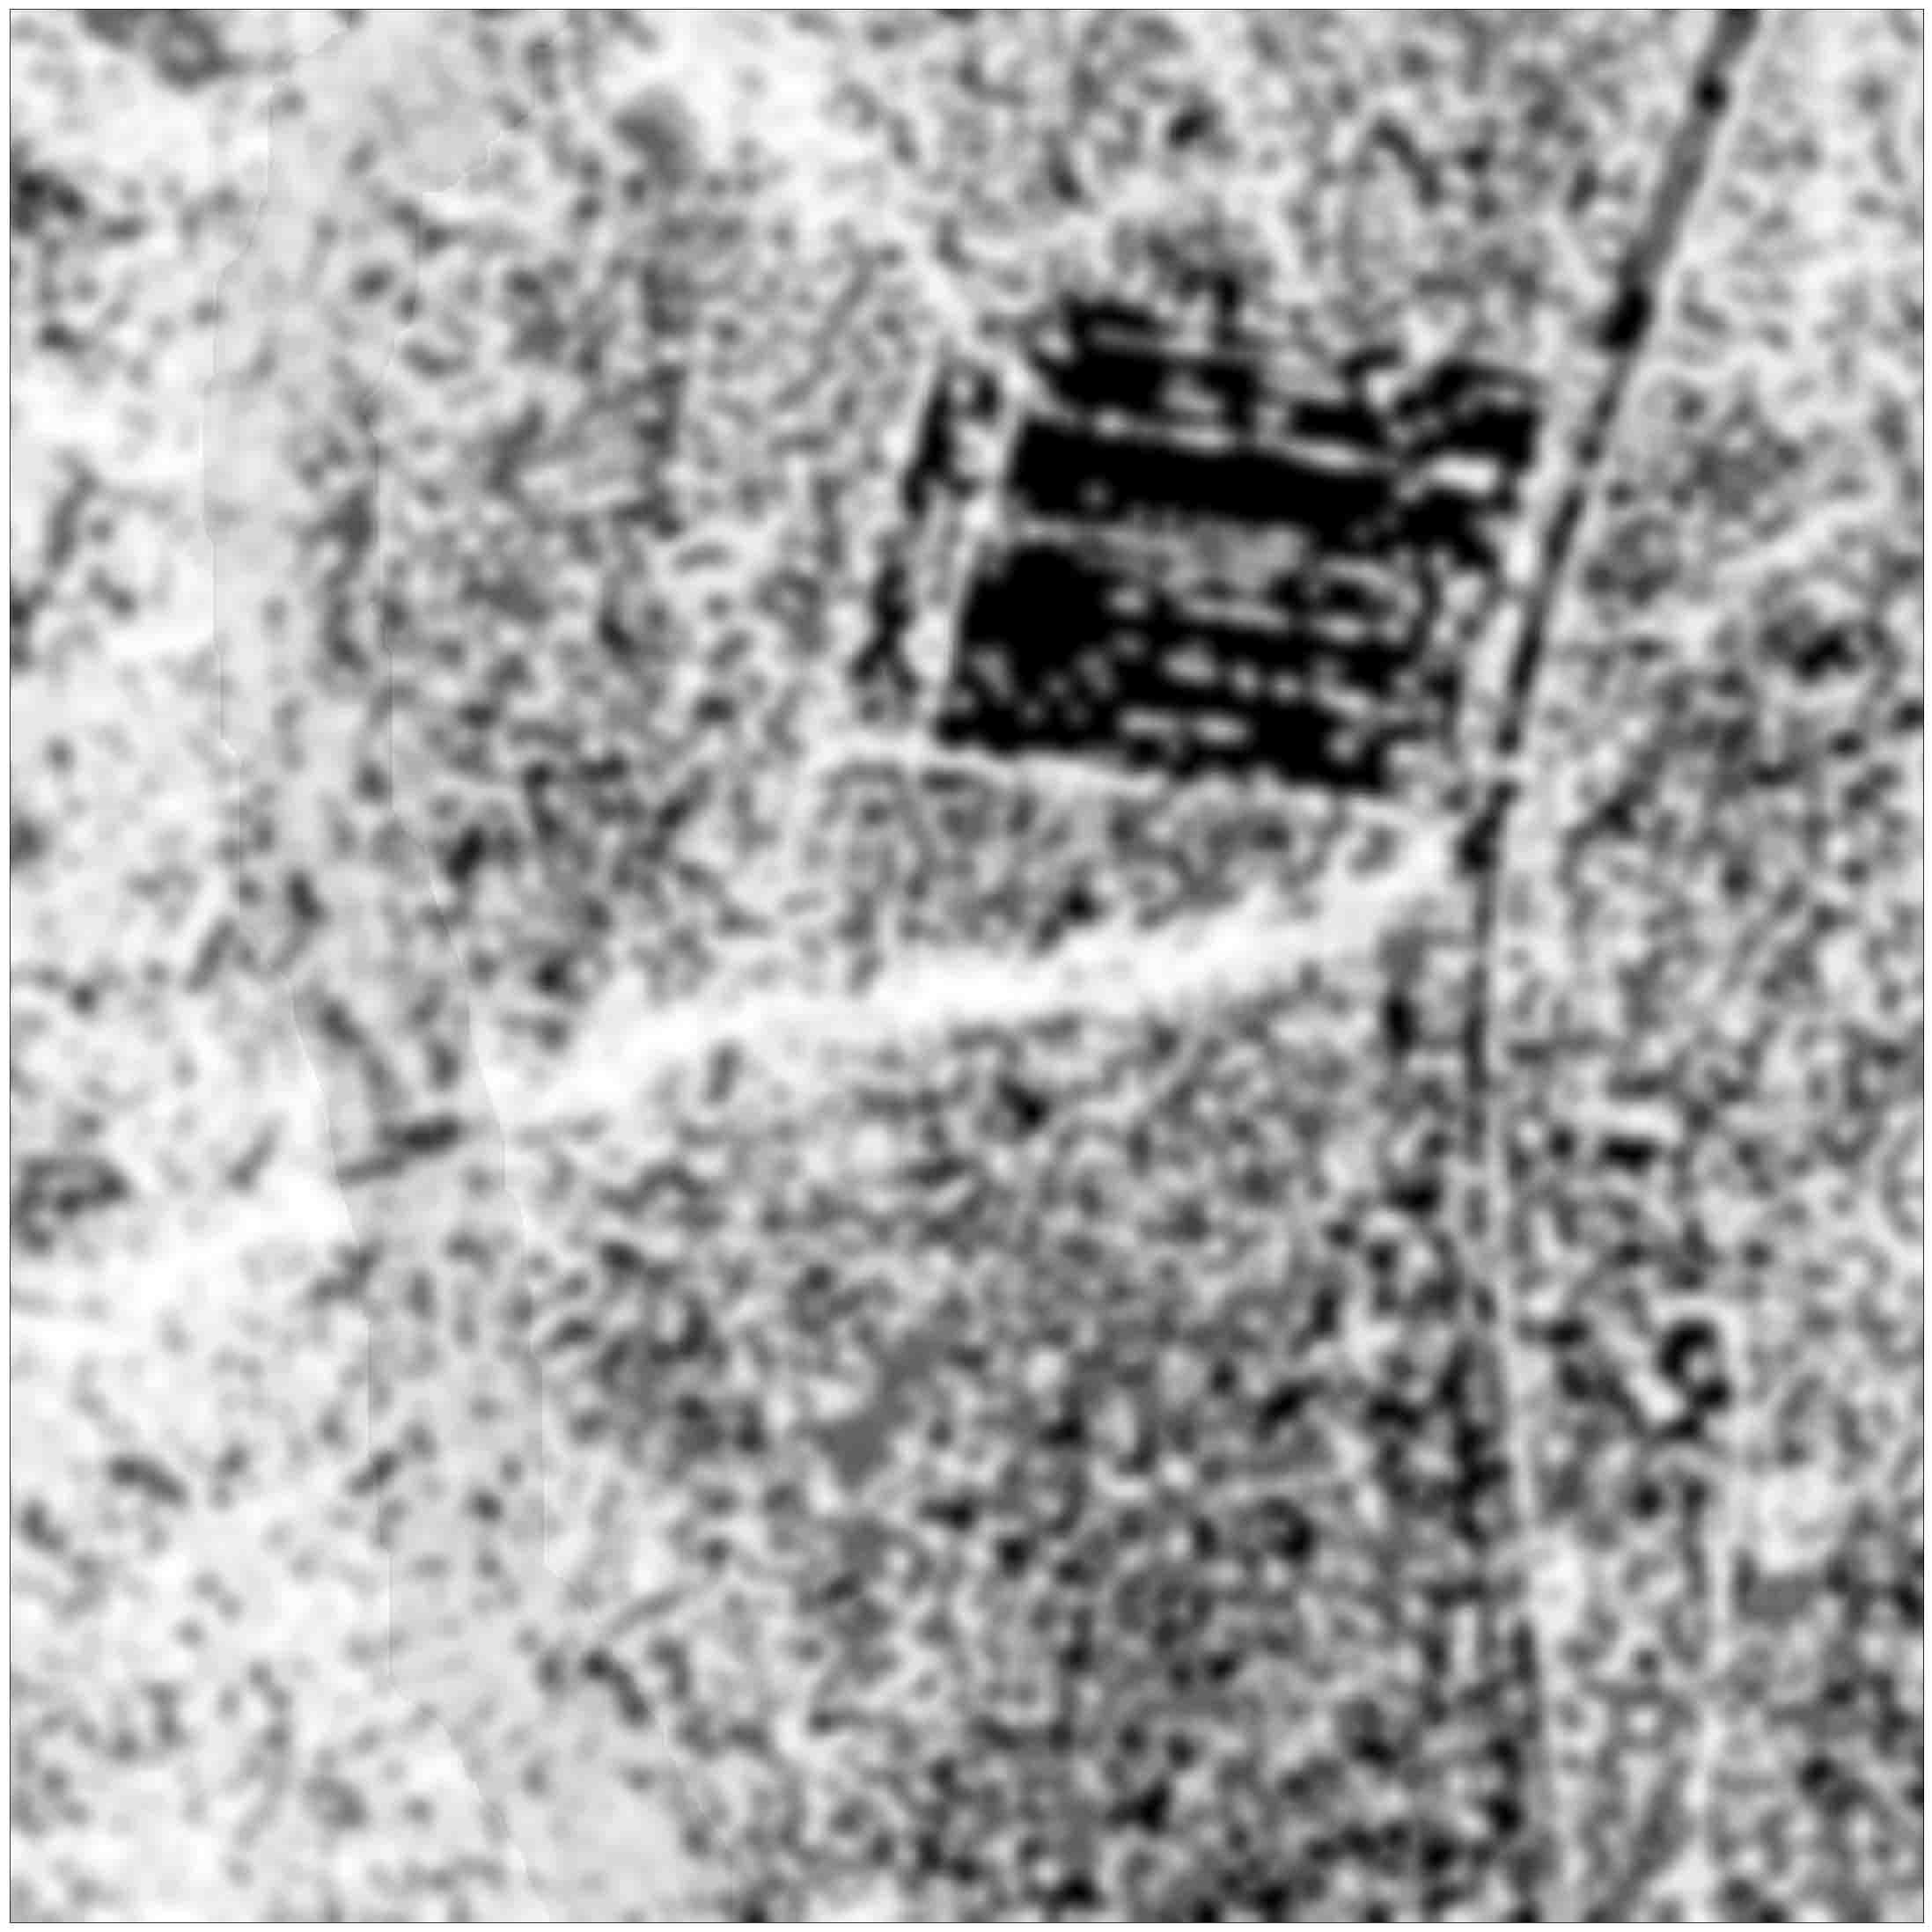
\includegraphics{./images/feature_f_lo.jpg}}}%%%
\DIFdelFL{\hspace{5pt}
    }\DIFdelendFL \DIFaddbeginFL \DIFaddFL{\hspace{5pt}
    }\subfigure[]{
        \resizebox*{4cm}{!}{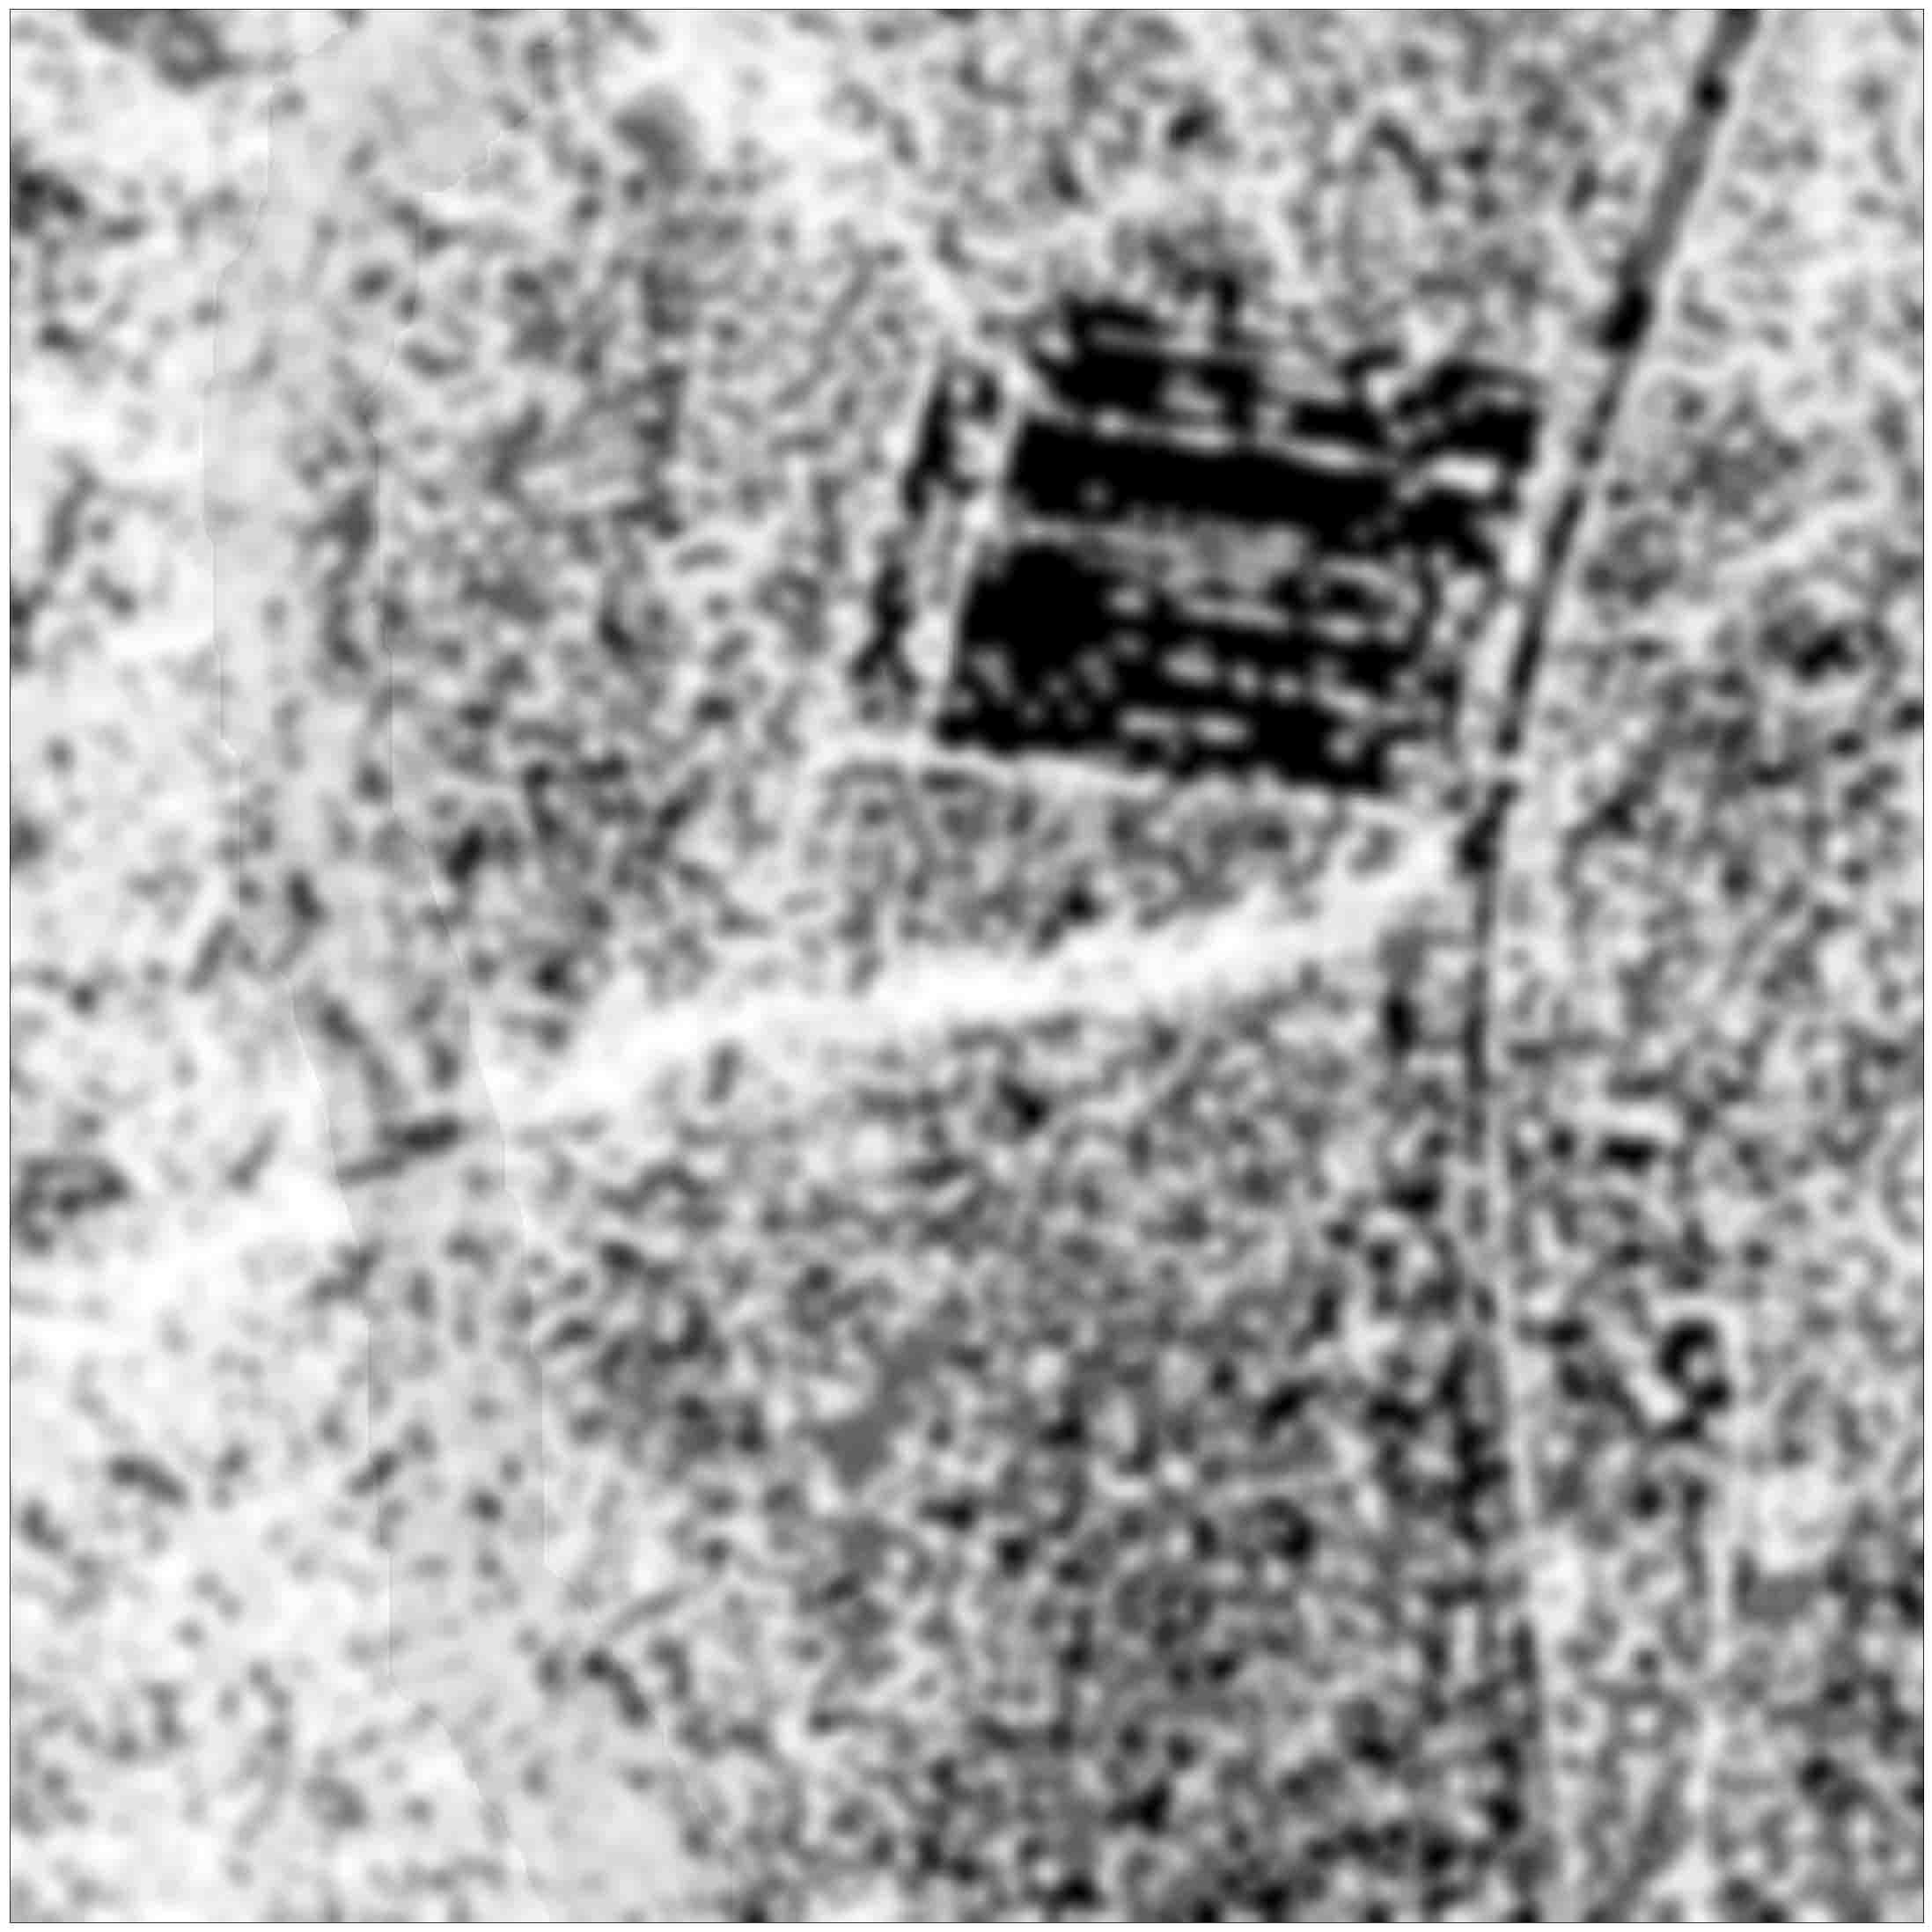
\includegraphics{./images/feature_f_lo.jpg}}}
    \DIFaddendFL \subfigure[]{
        \resizebox*{4cm}{!}{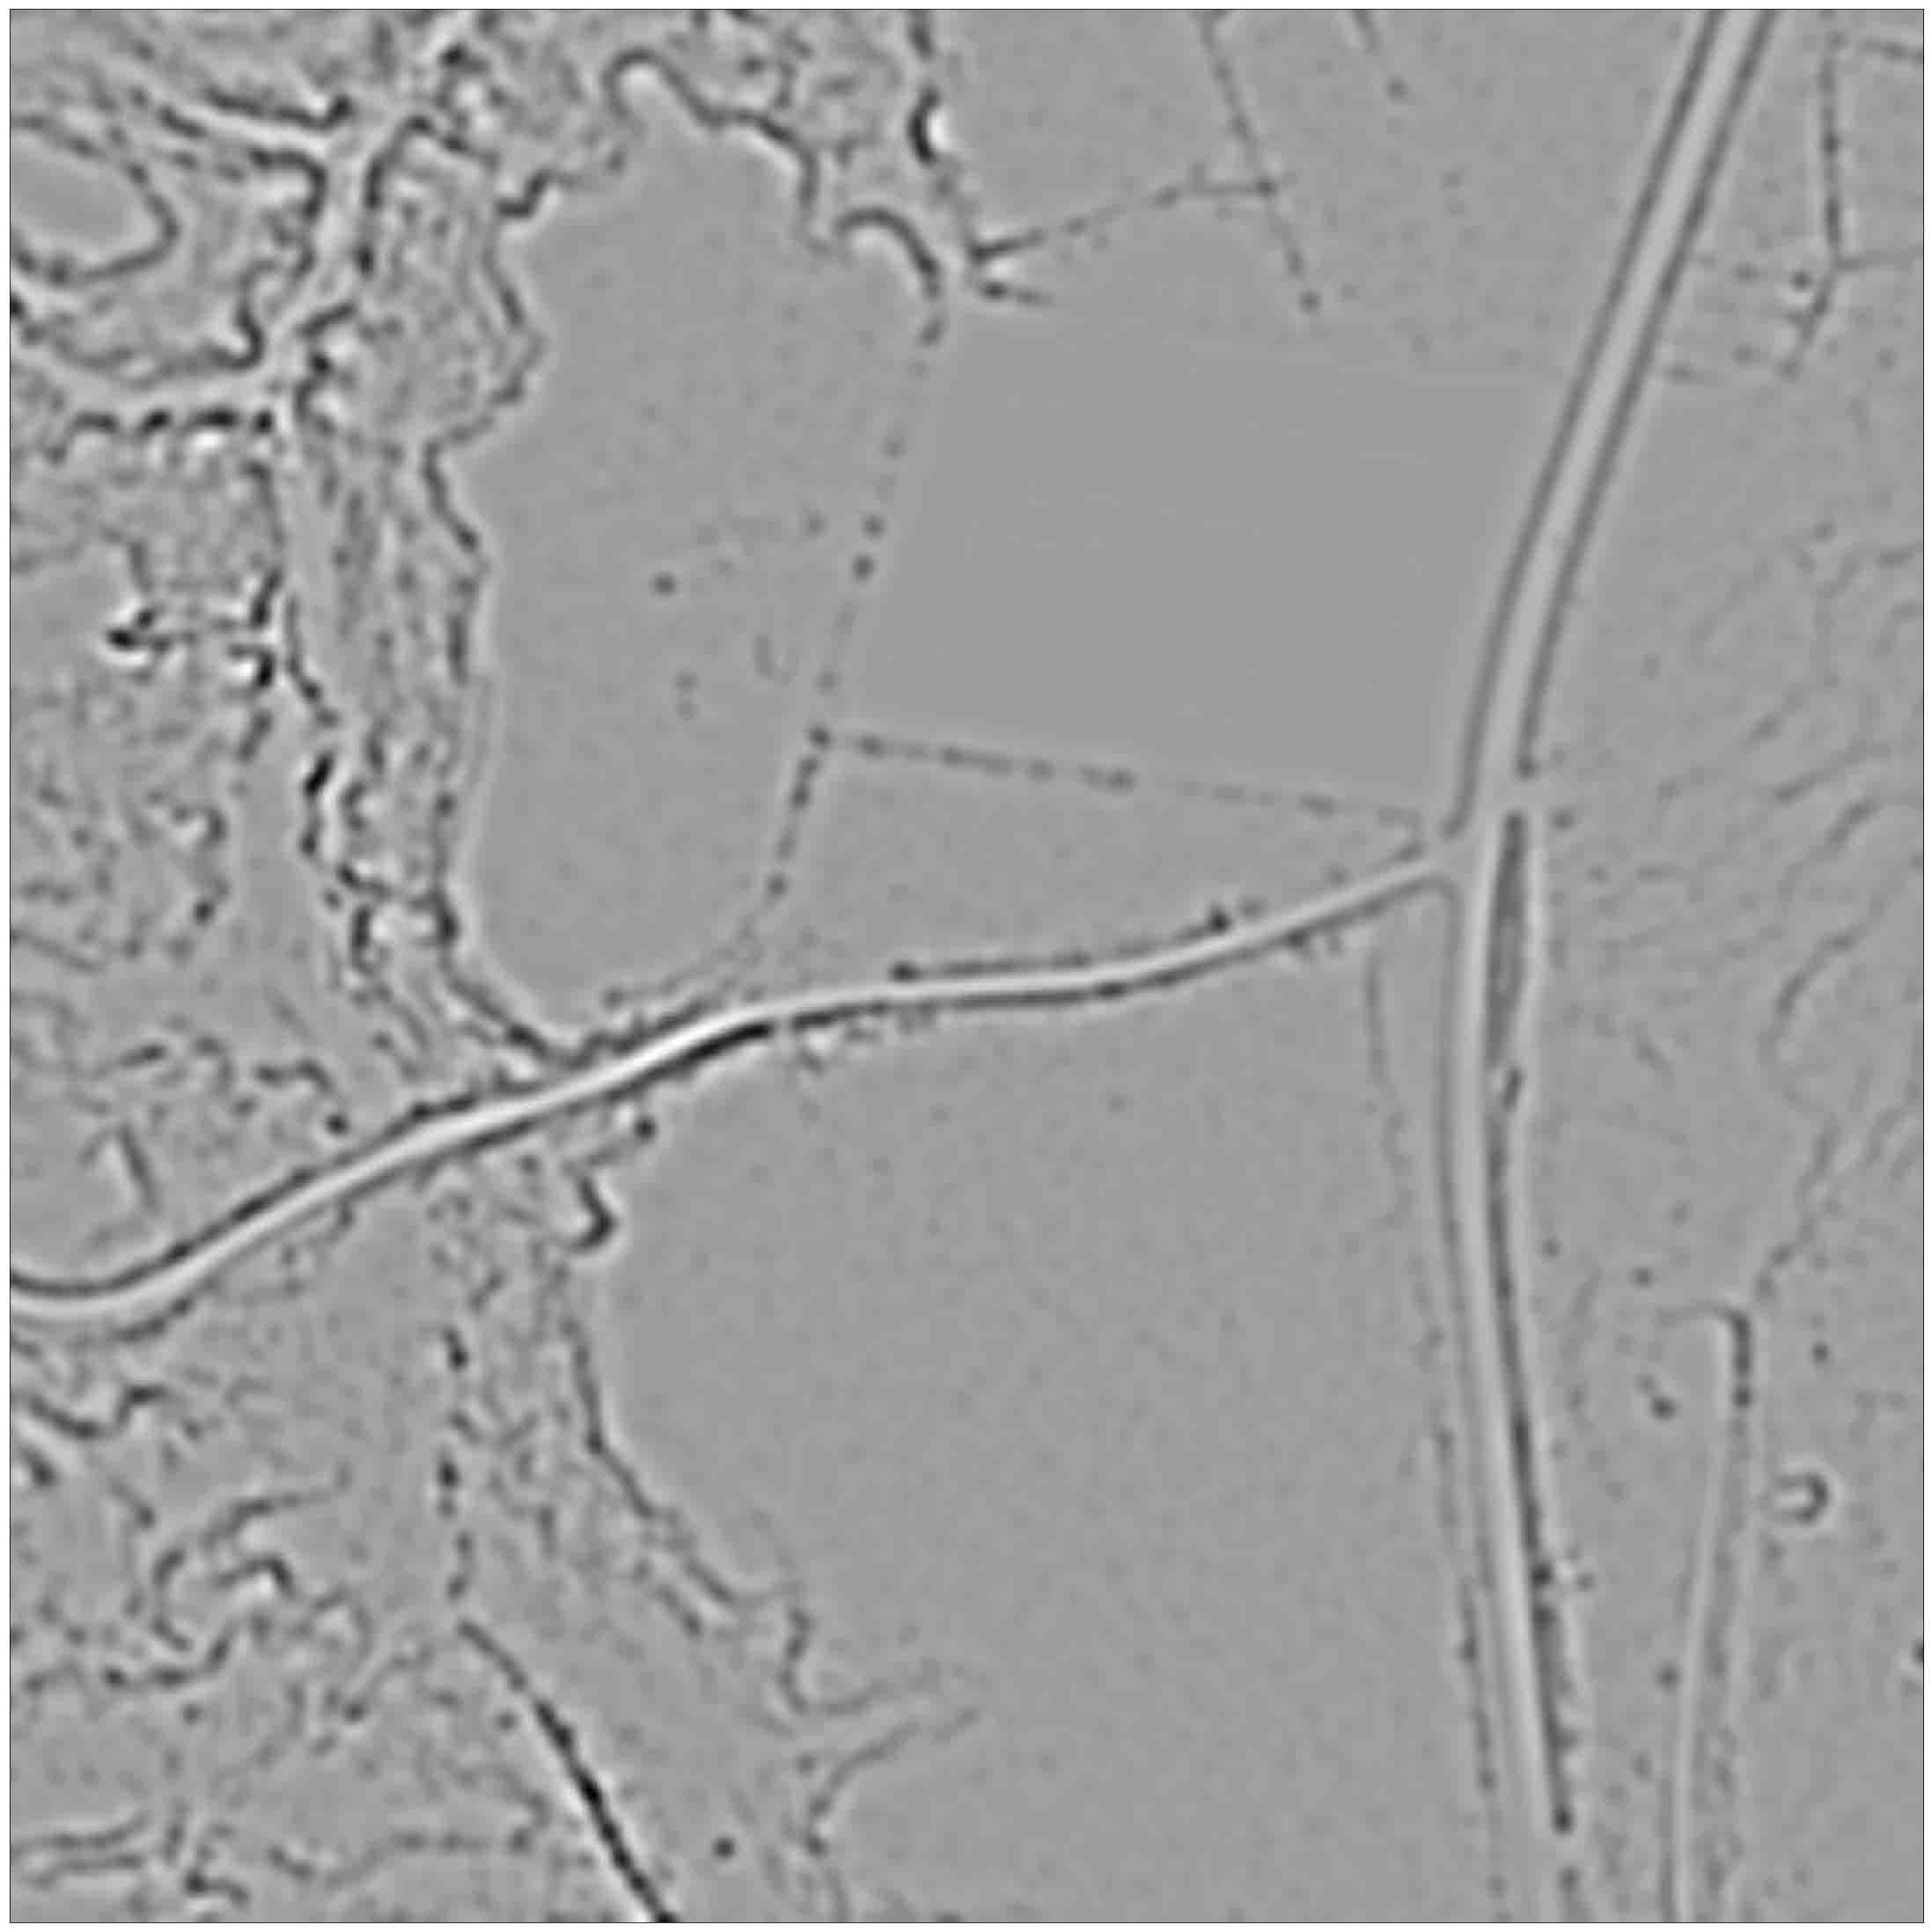
\includegraphics{./images/feature_g_lo.jpg}}}\hspace{5pt}
    \subfigure[]{
        \resizebox*{4cm}{!}{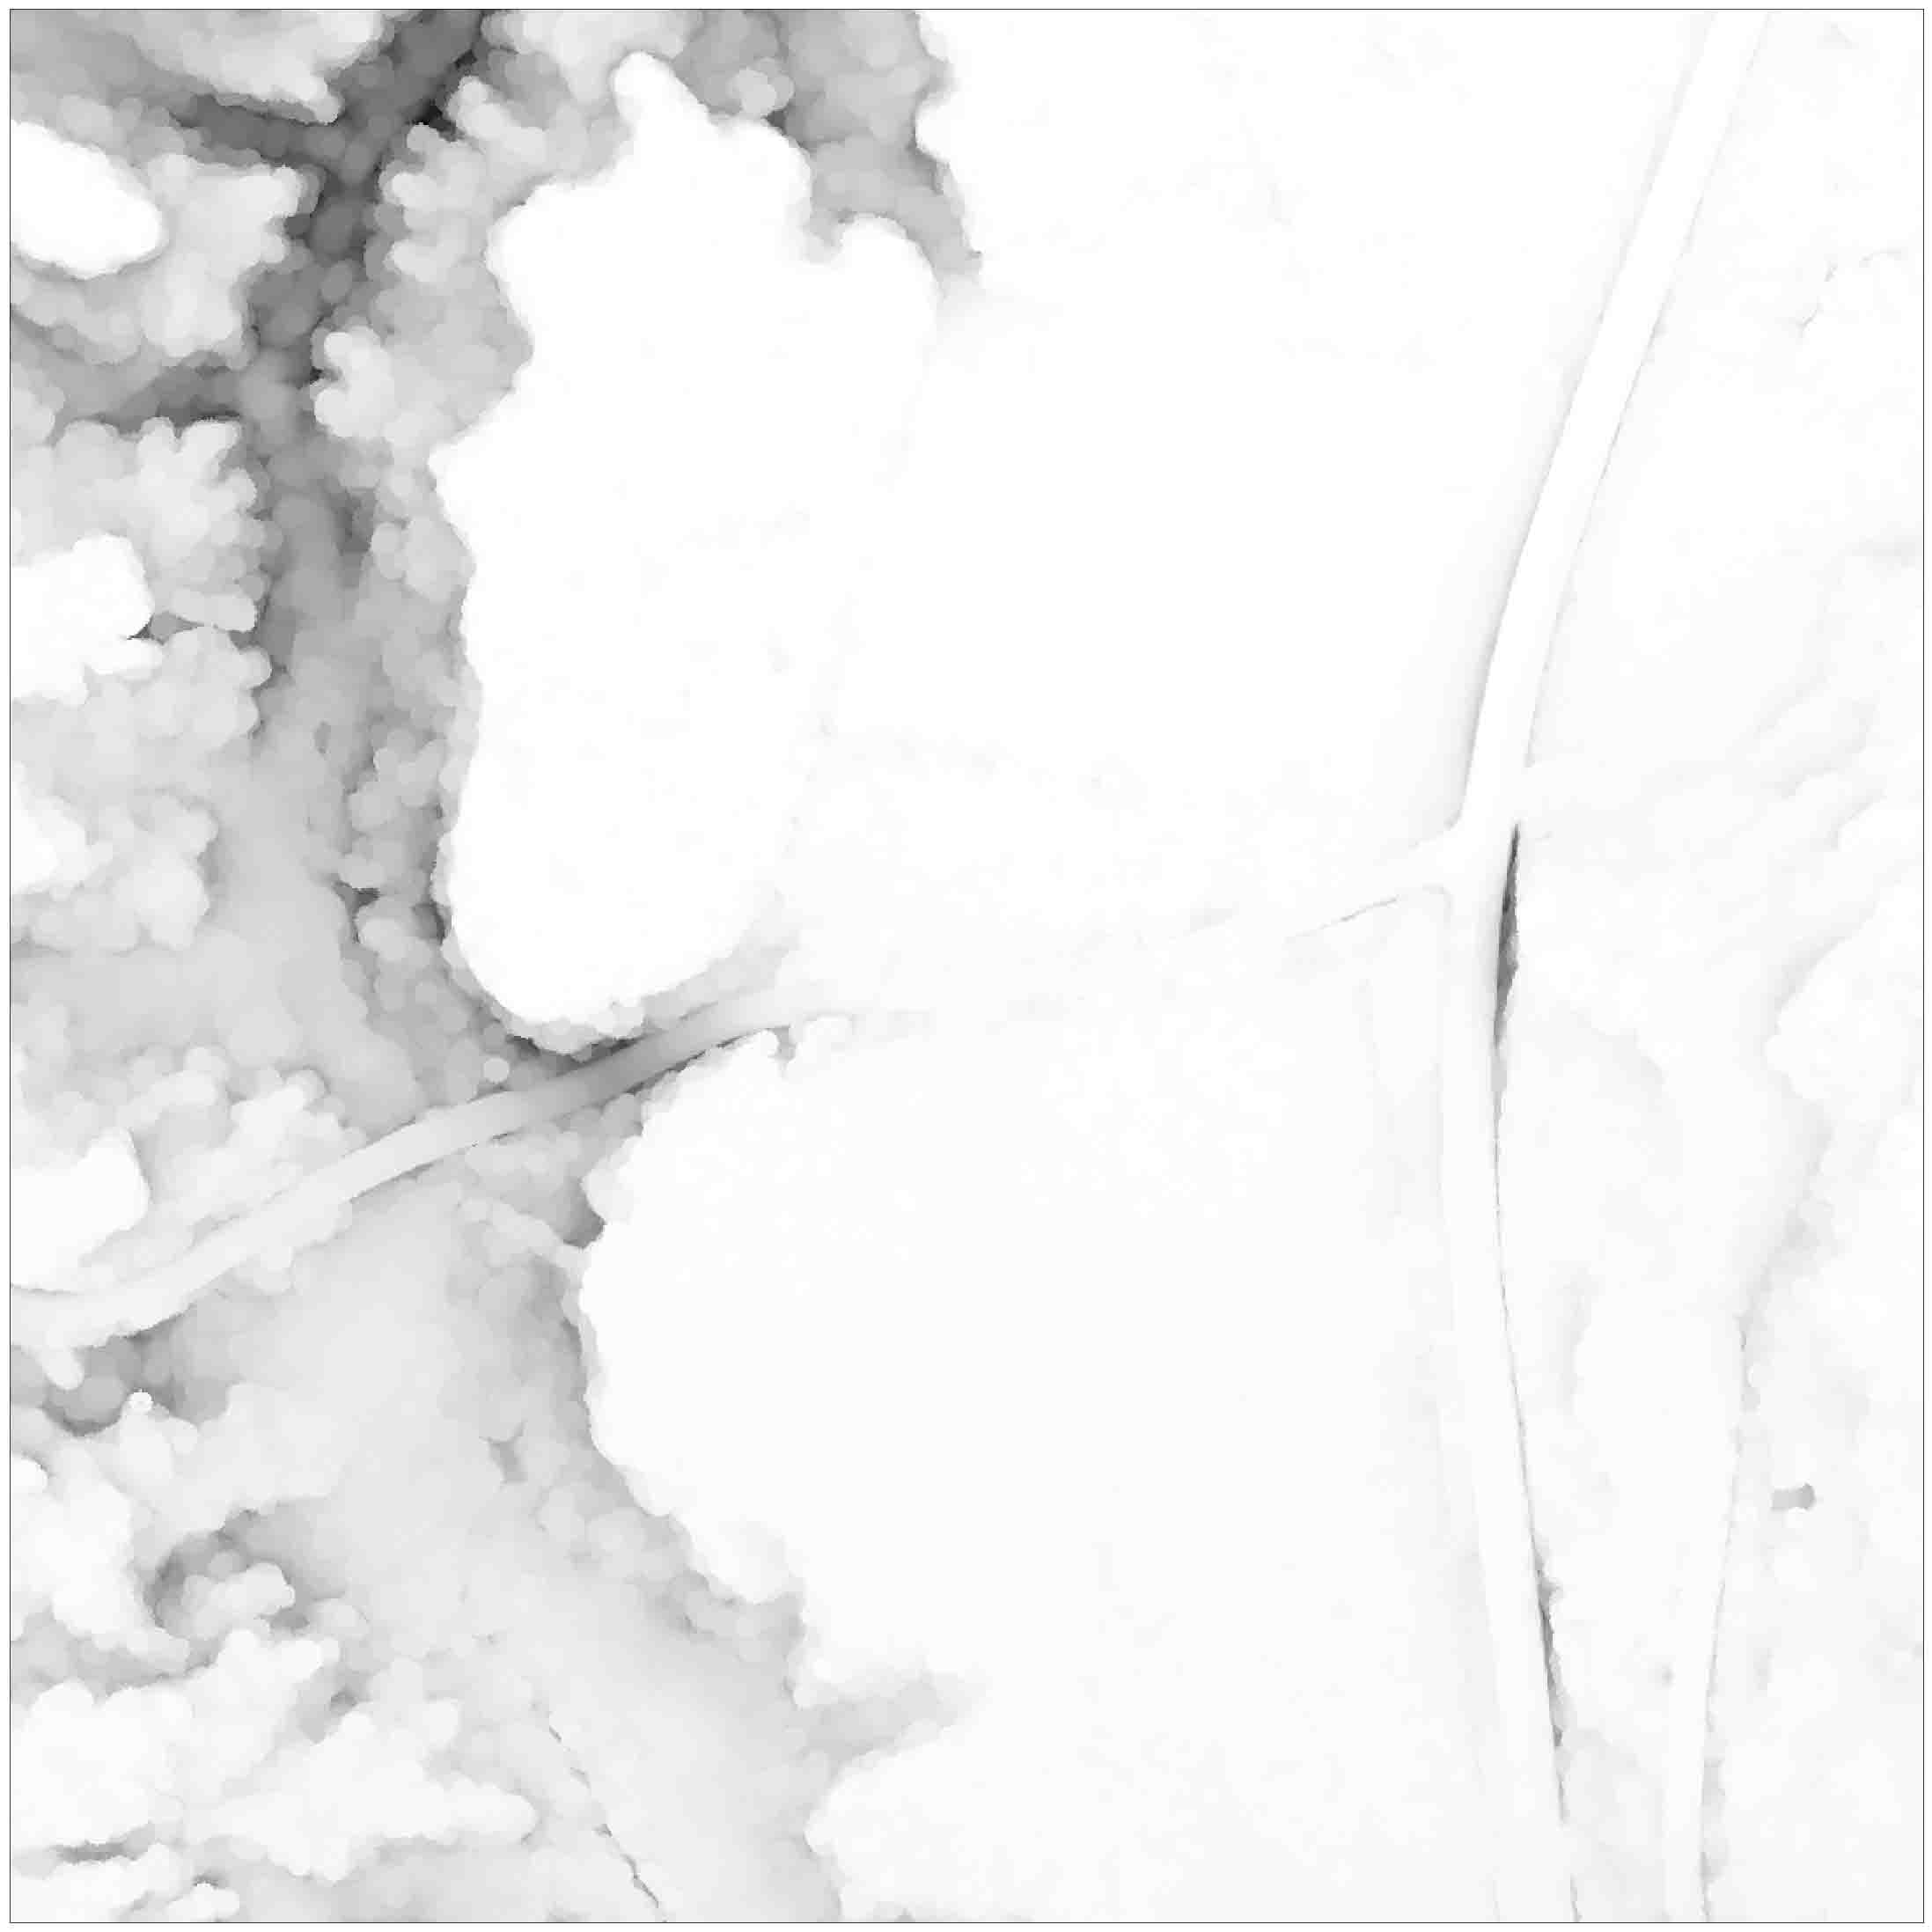
\includegraphics{./images/feature_h_lo.jpg}}}
    \subfigure[]{
        \resizebox*{4cm}{!}{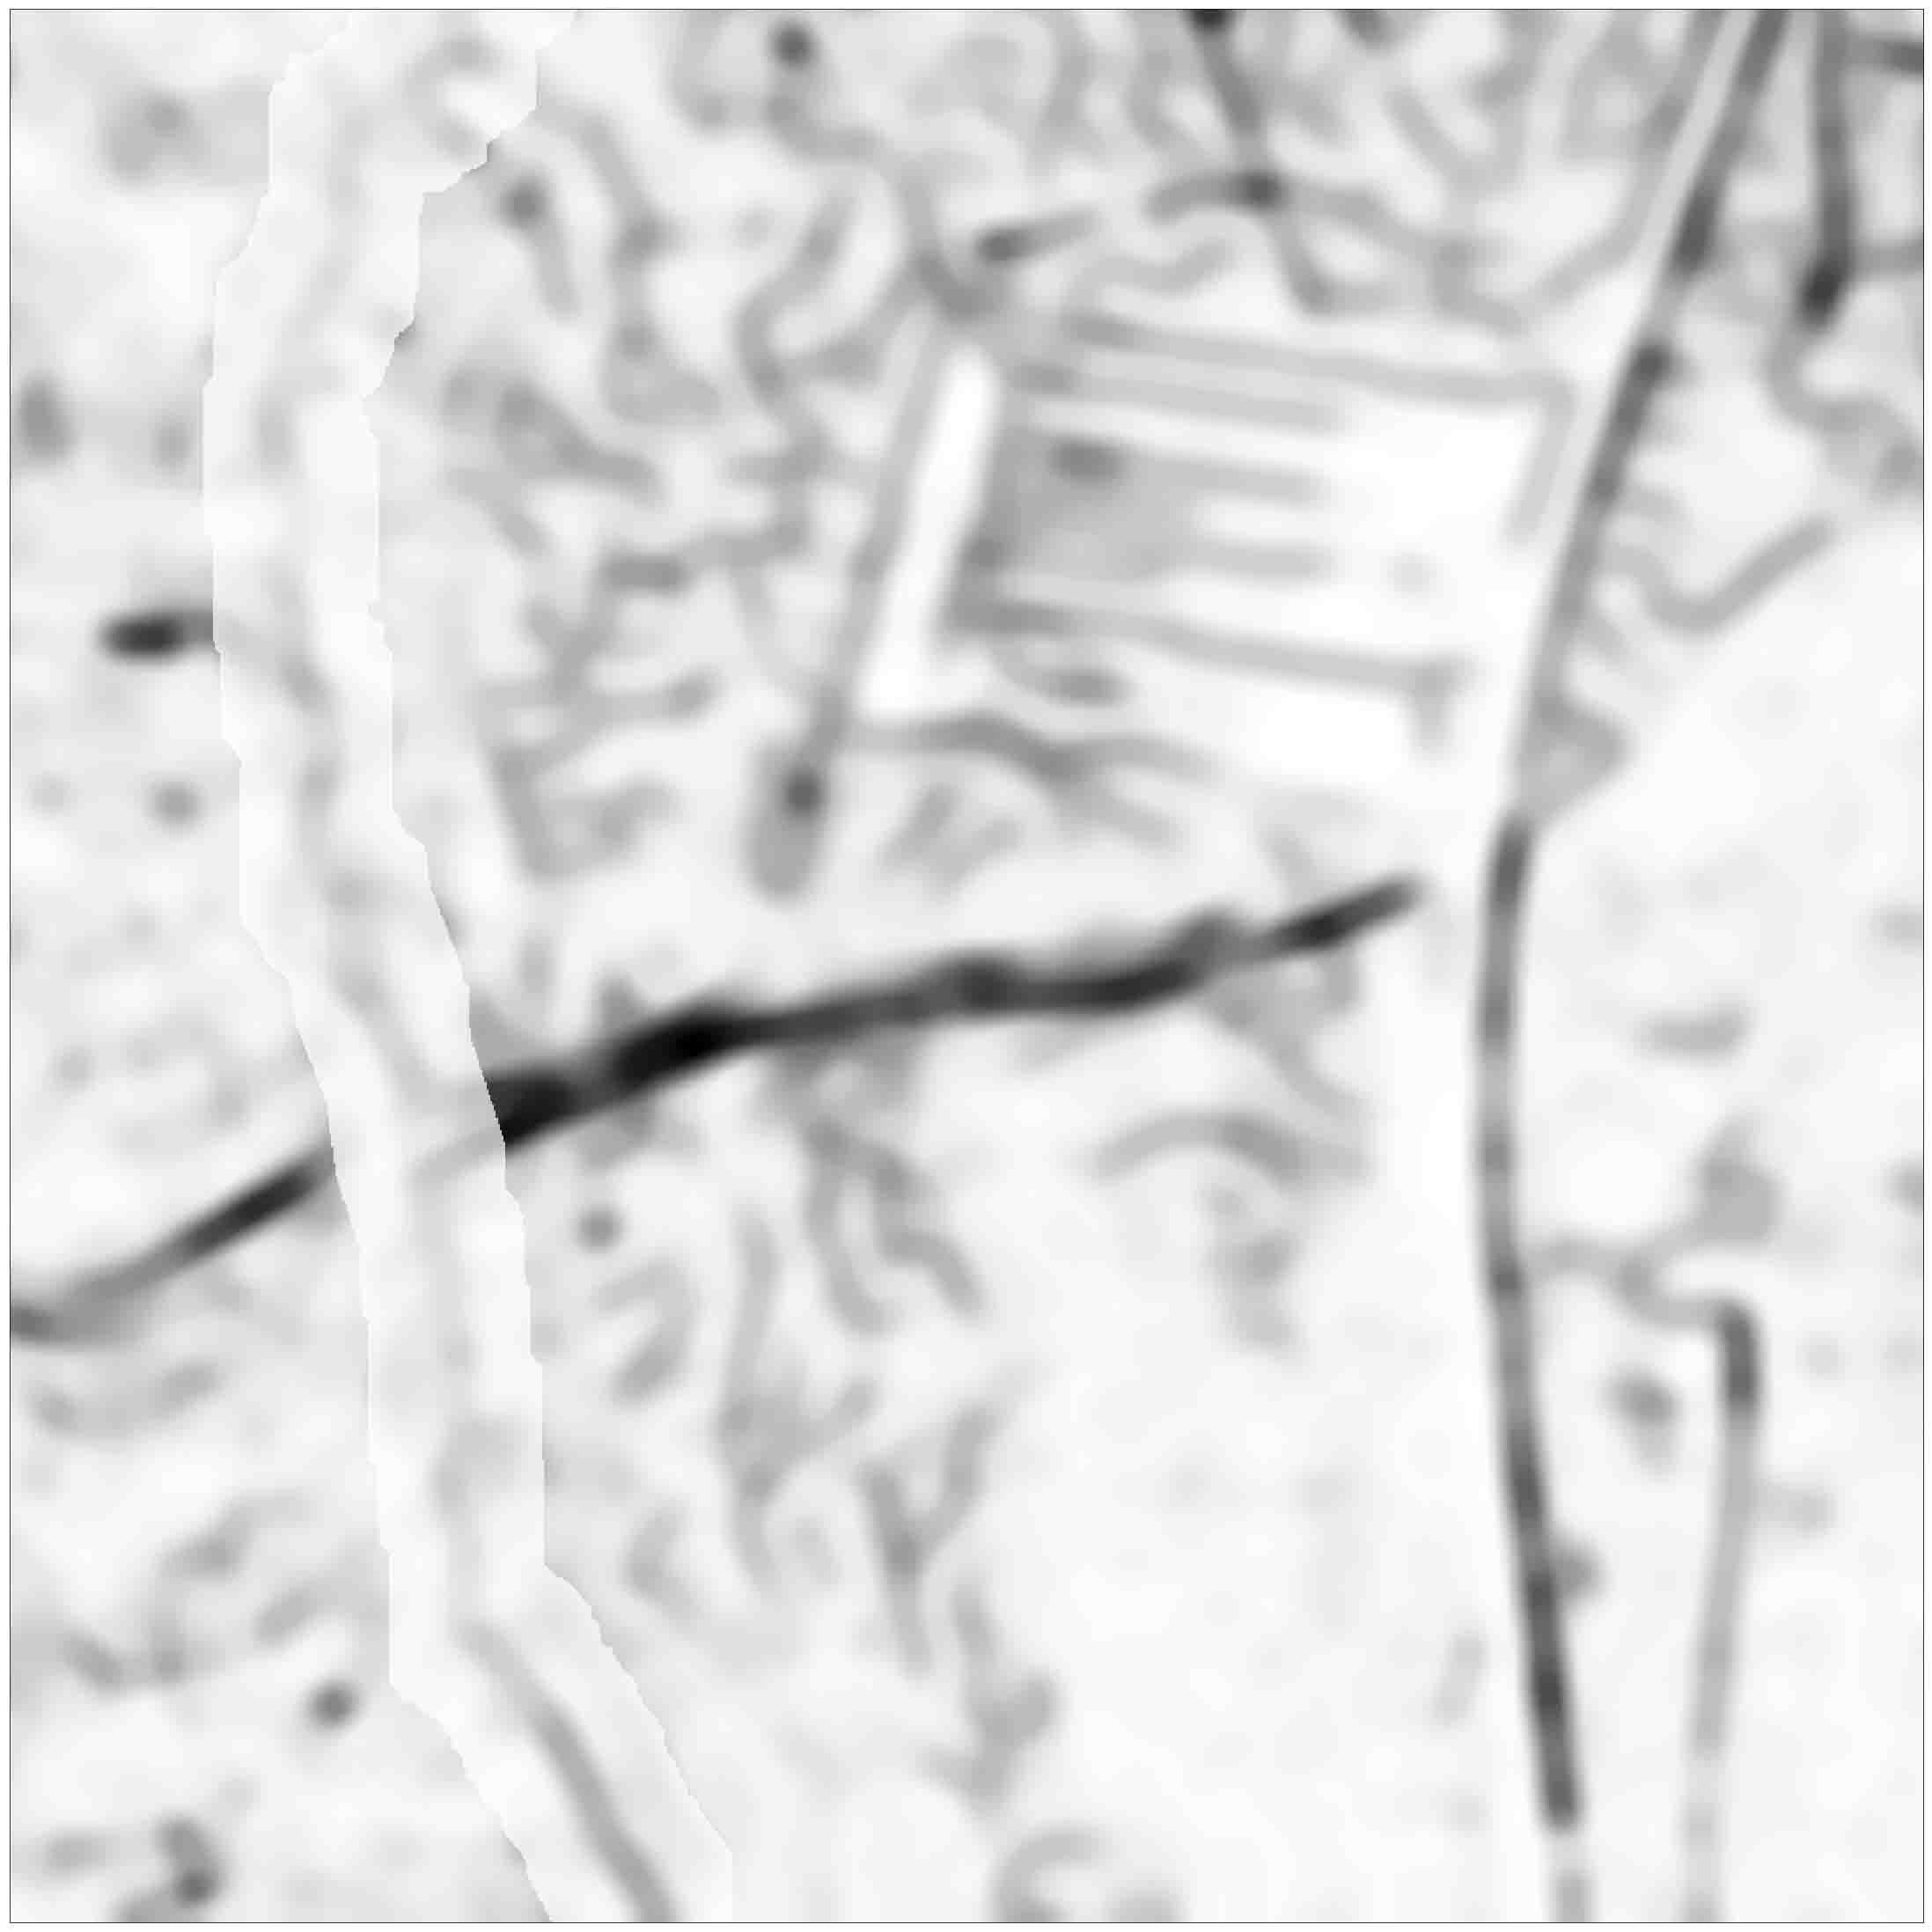
\includegraphics{./images/feature_i_lo.jpg}}}
    \DIFdelbeginFL \DIFdelFL{\hspace{5pt}
    }%DIFDELCMD < \subfigure[]{
%DIFDELCMD <         \resizebox*{4cm}{!}{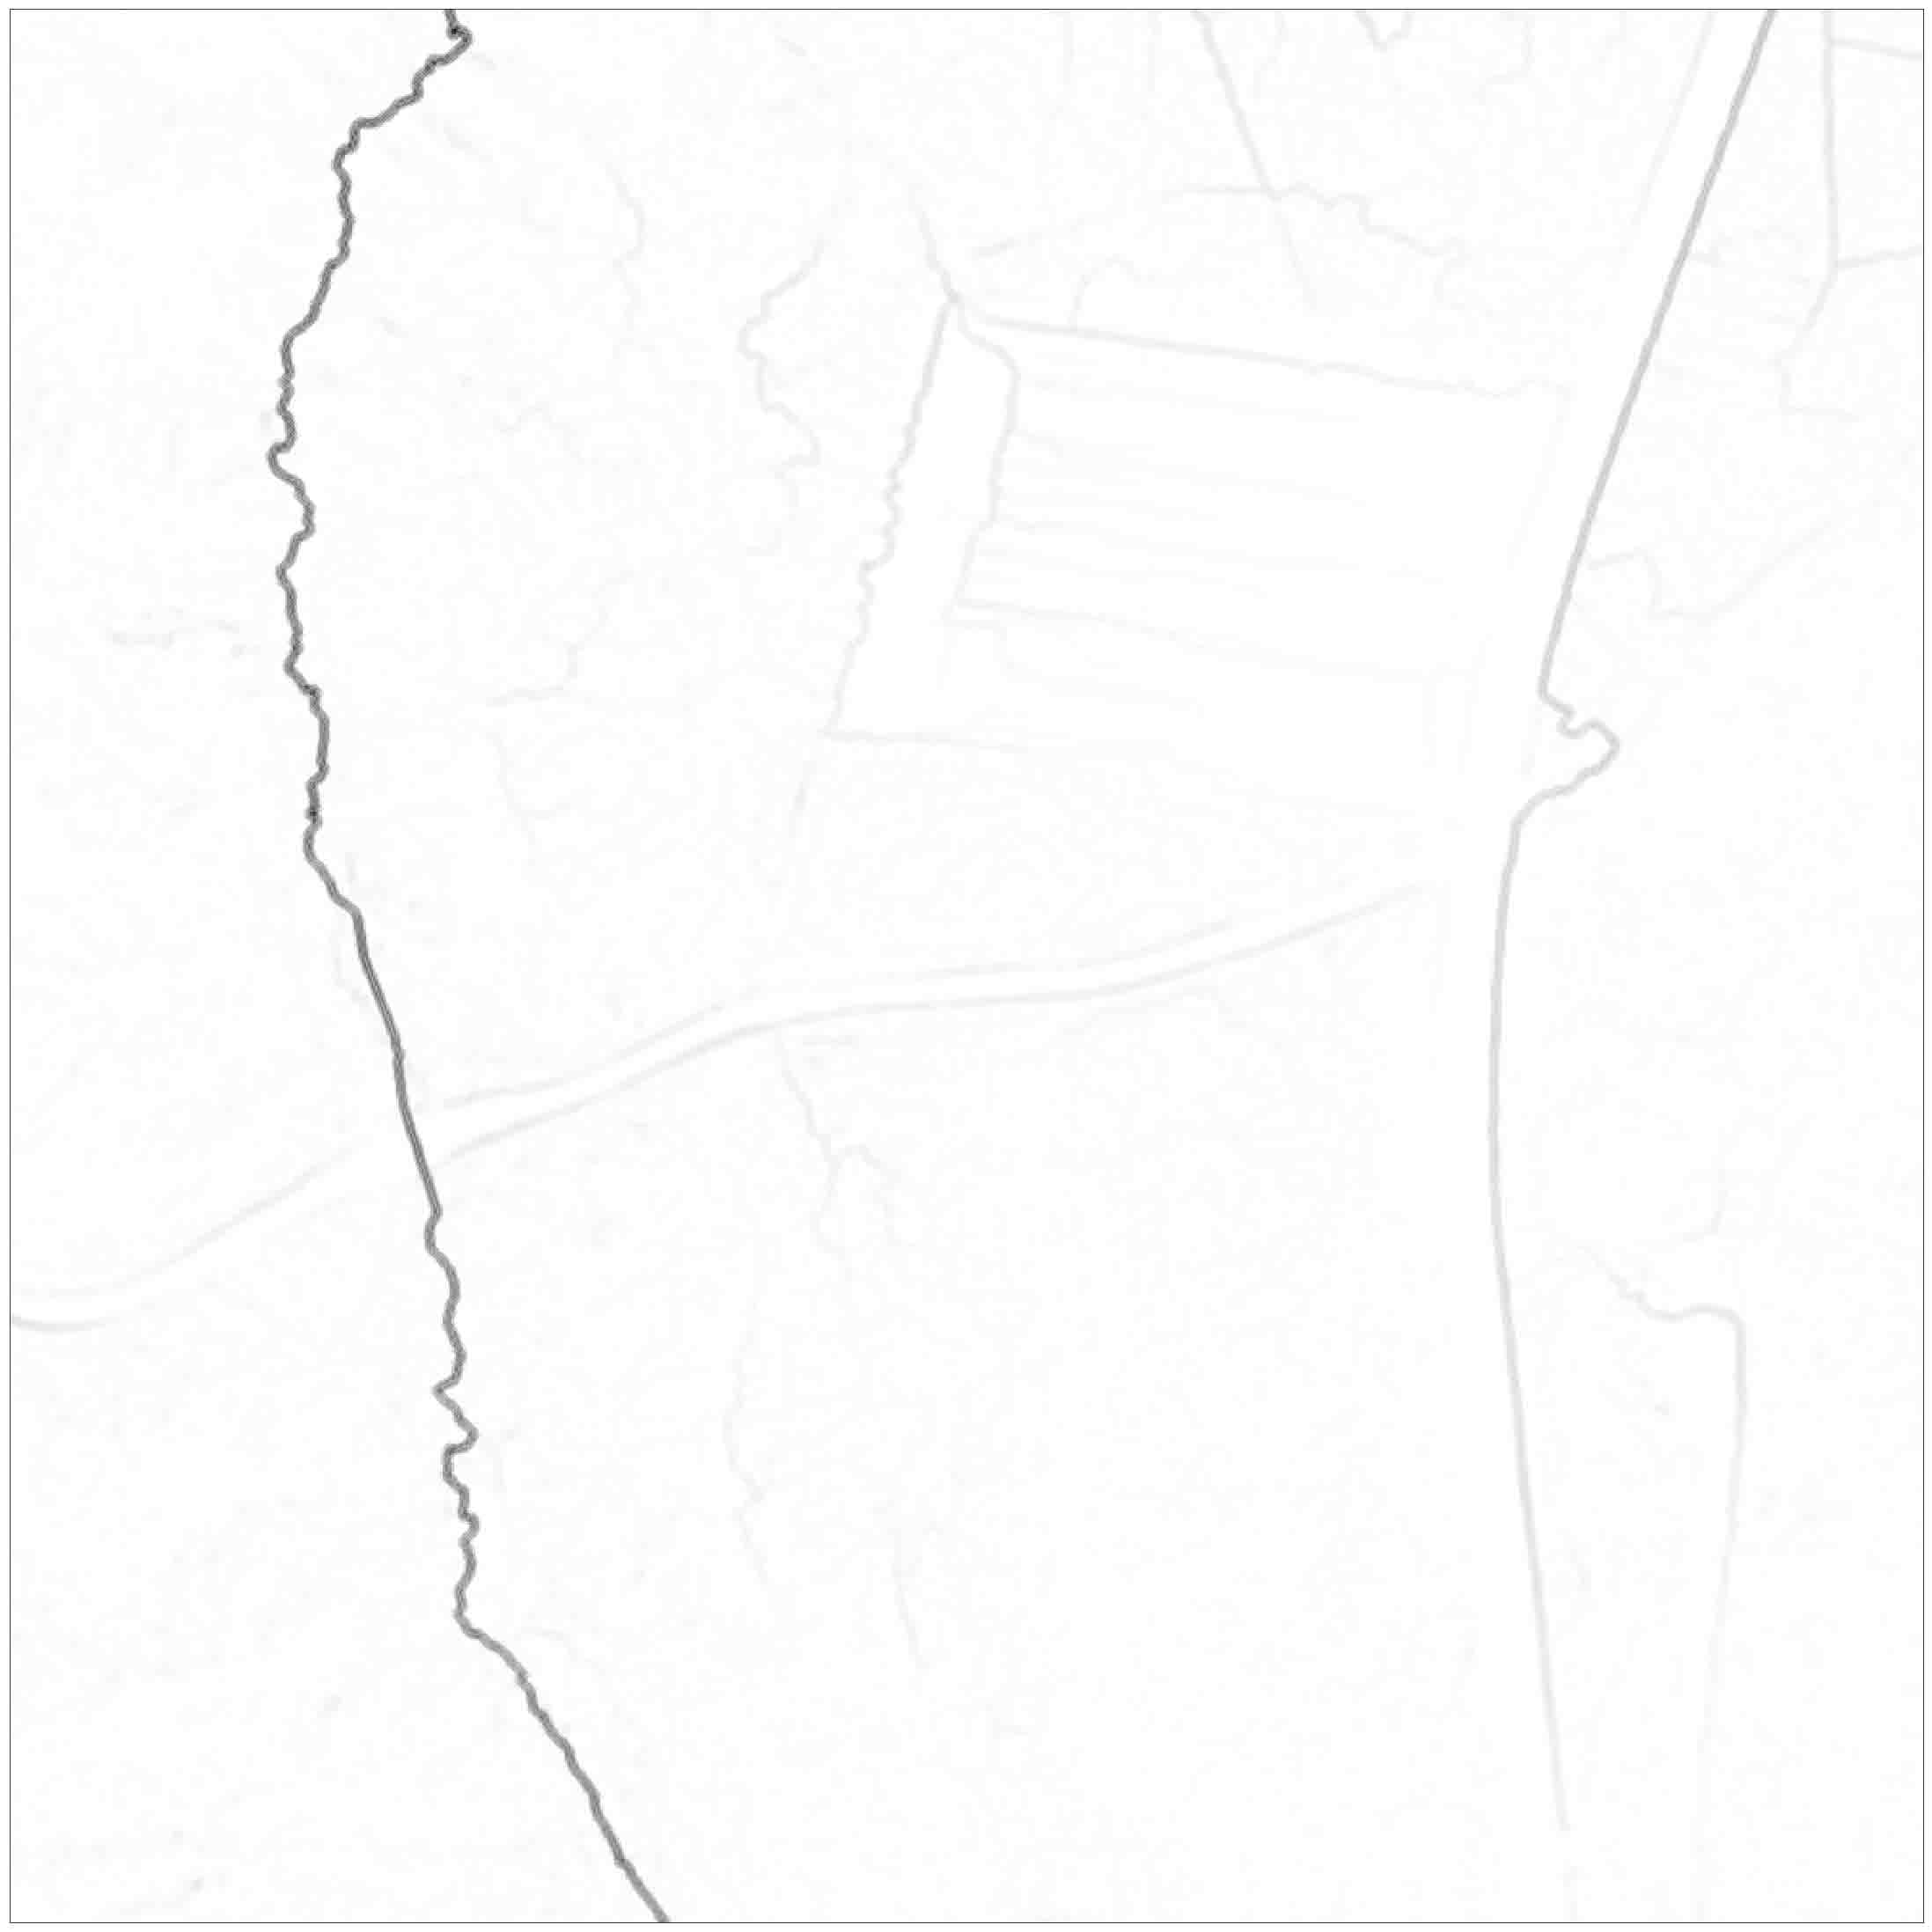
\includegraphics{./images/feature_j_lo.jpg}}}%%%
\DIFdelFL{\hspace{5pt}
    }%DIFDELCMD < \subfigure[]{
%DIFDELCMD <         \resizebox*{4cm}{!}{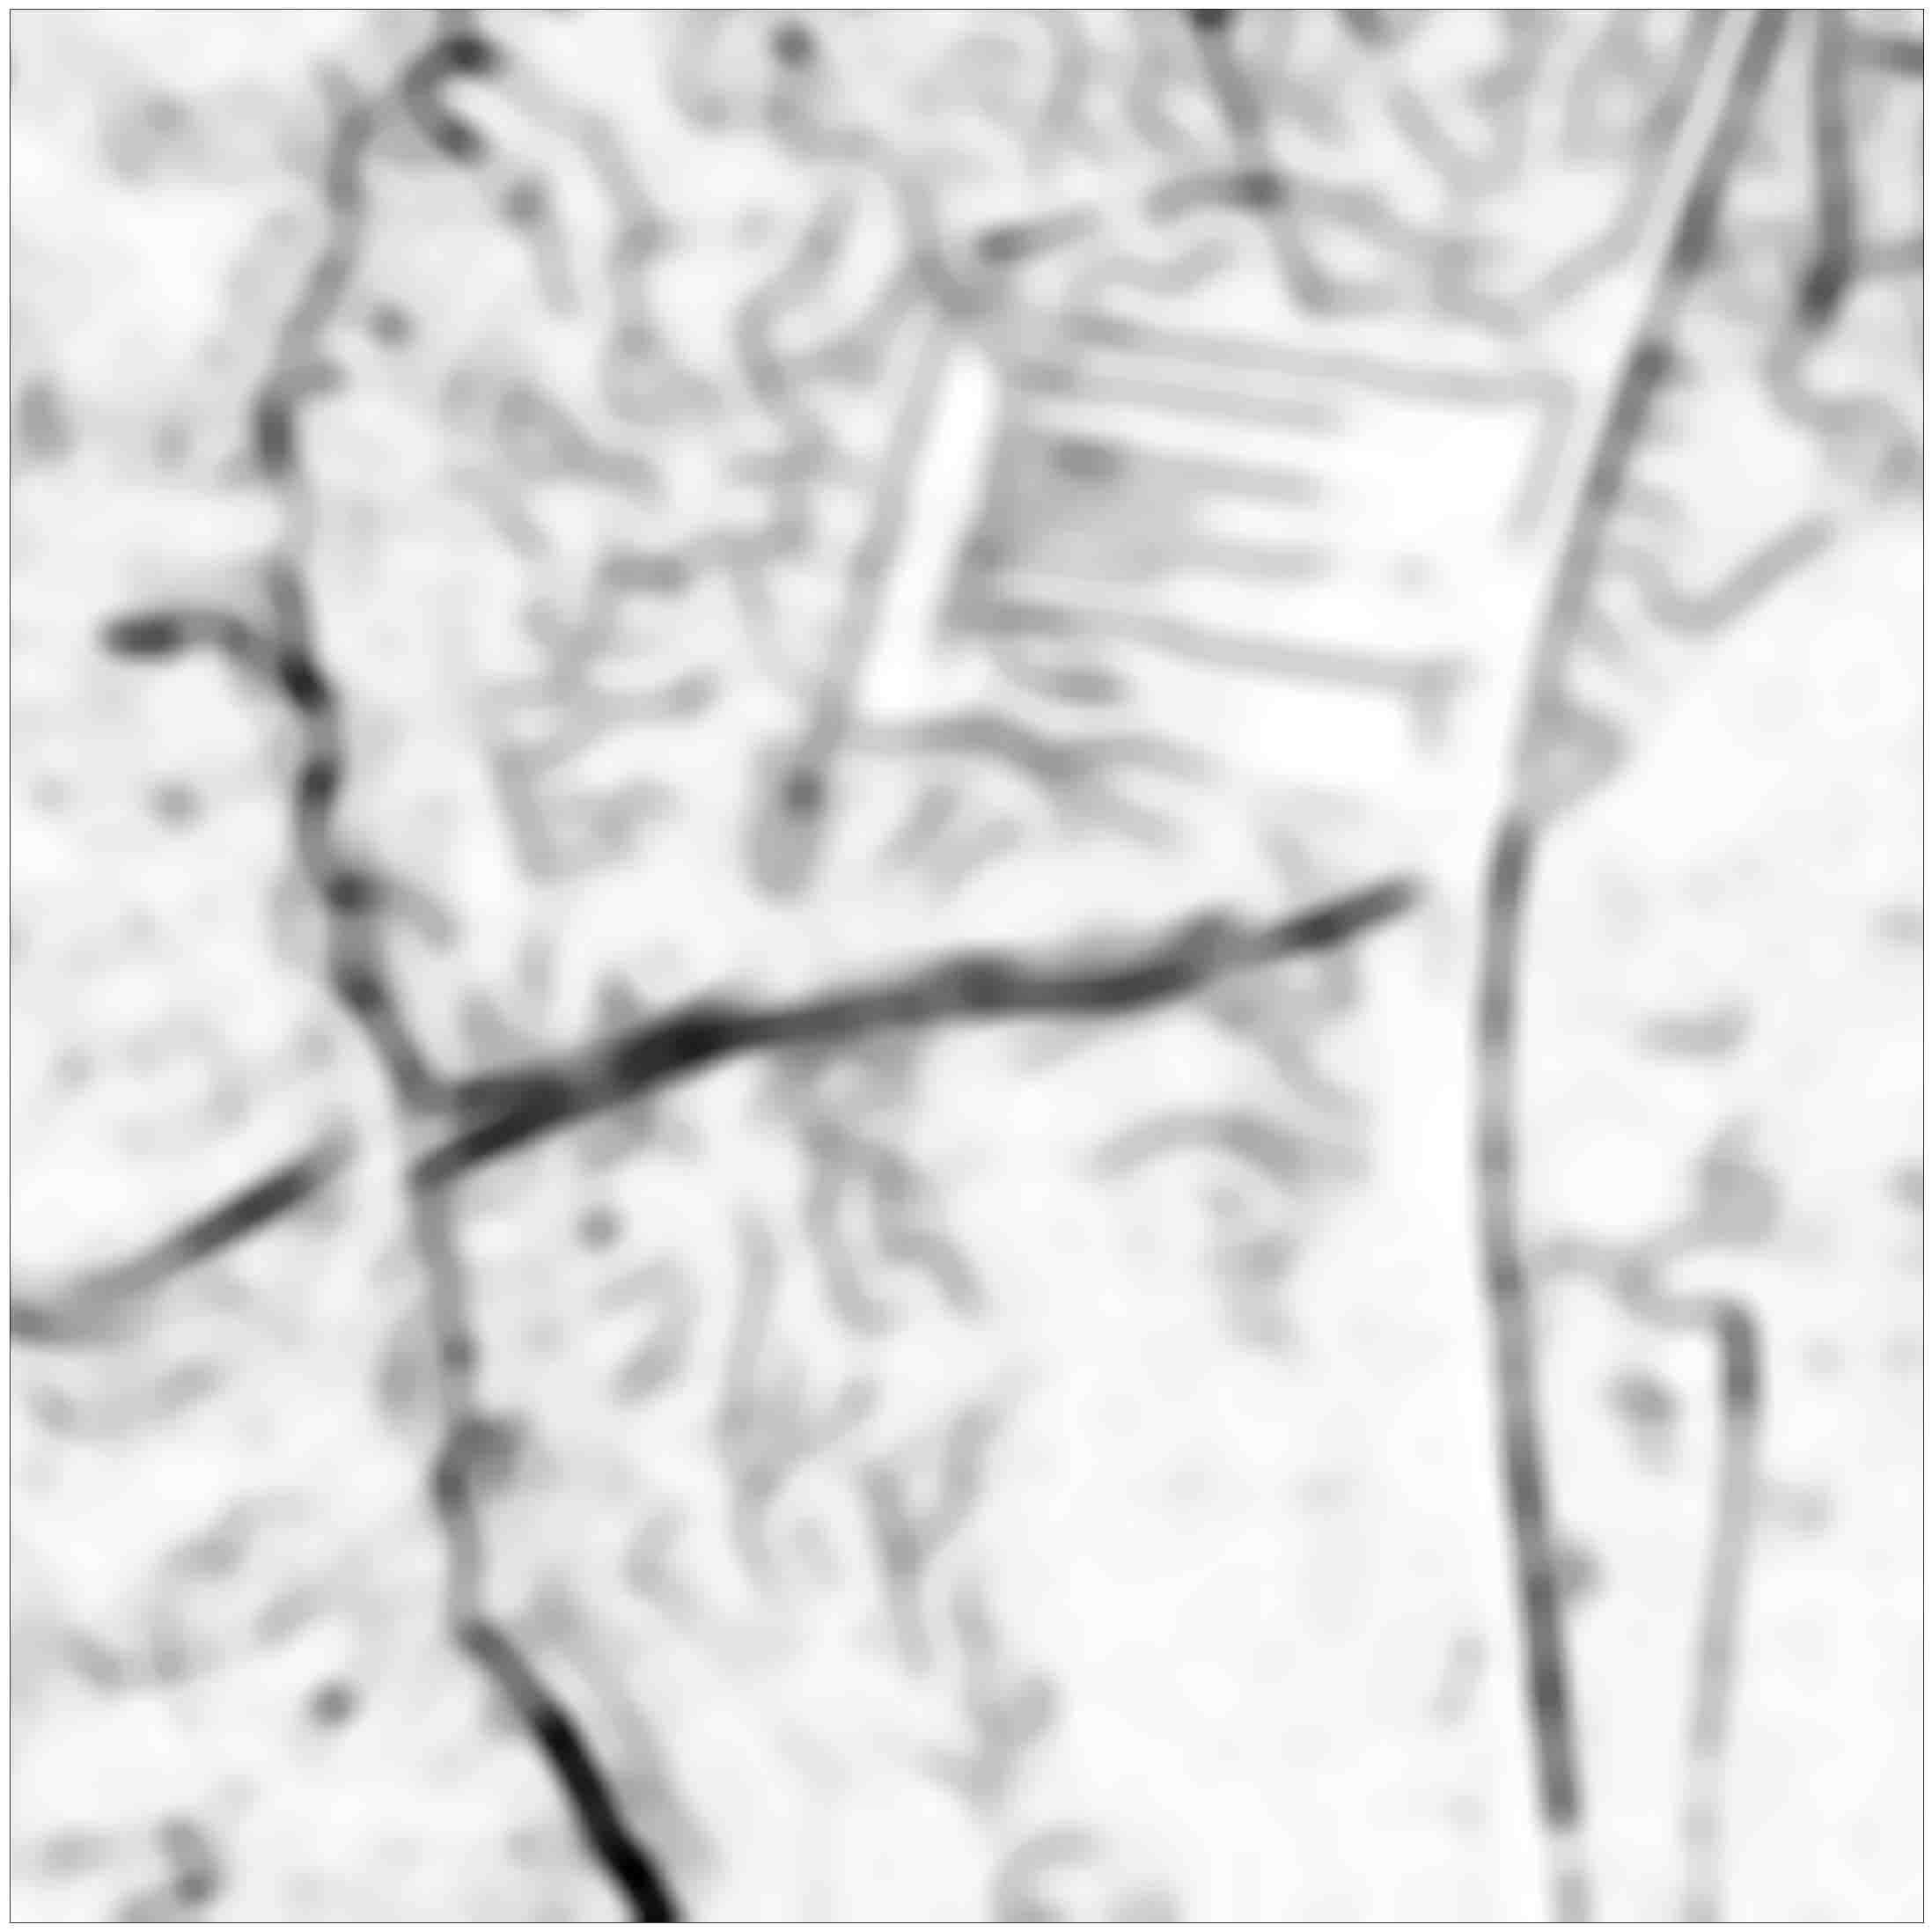
\includegraphics{./images/feature_k_lo.jpg}}}
%DIFDELCMD <     \subfigure[]{
%DIFDELCMD <         \resizebox*{4cm}{!}{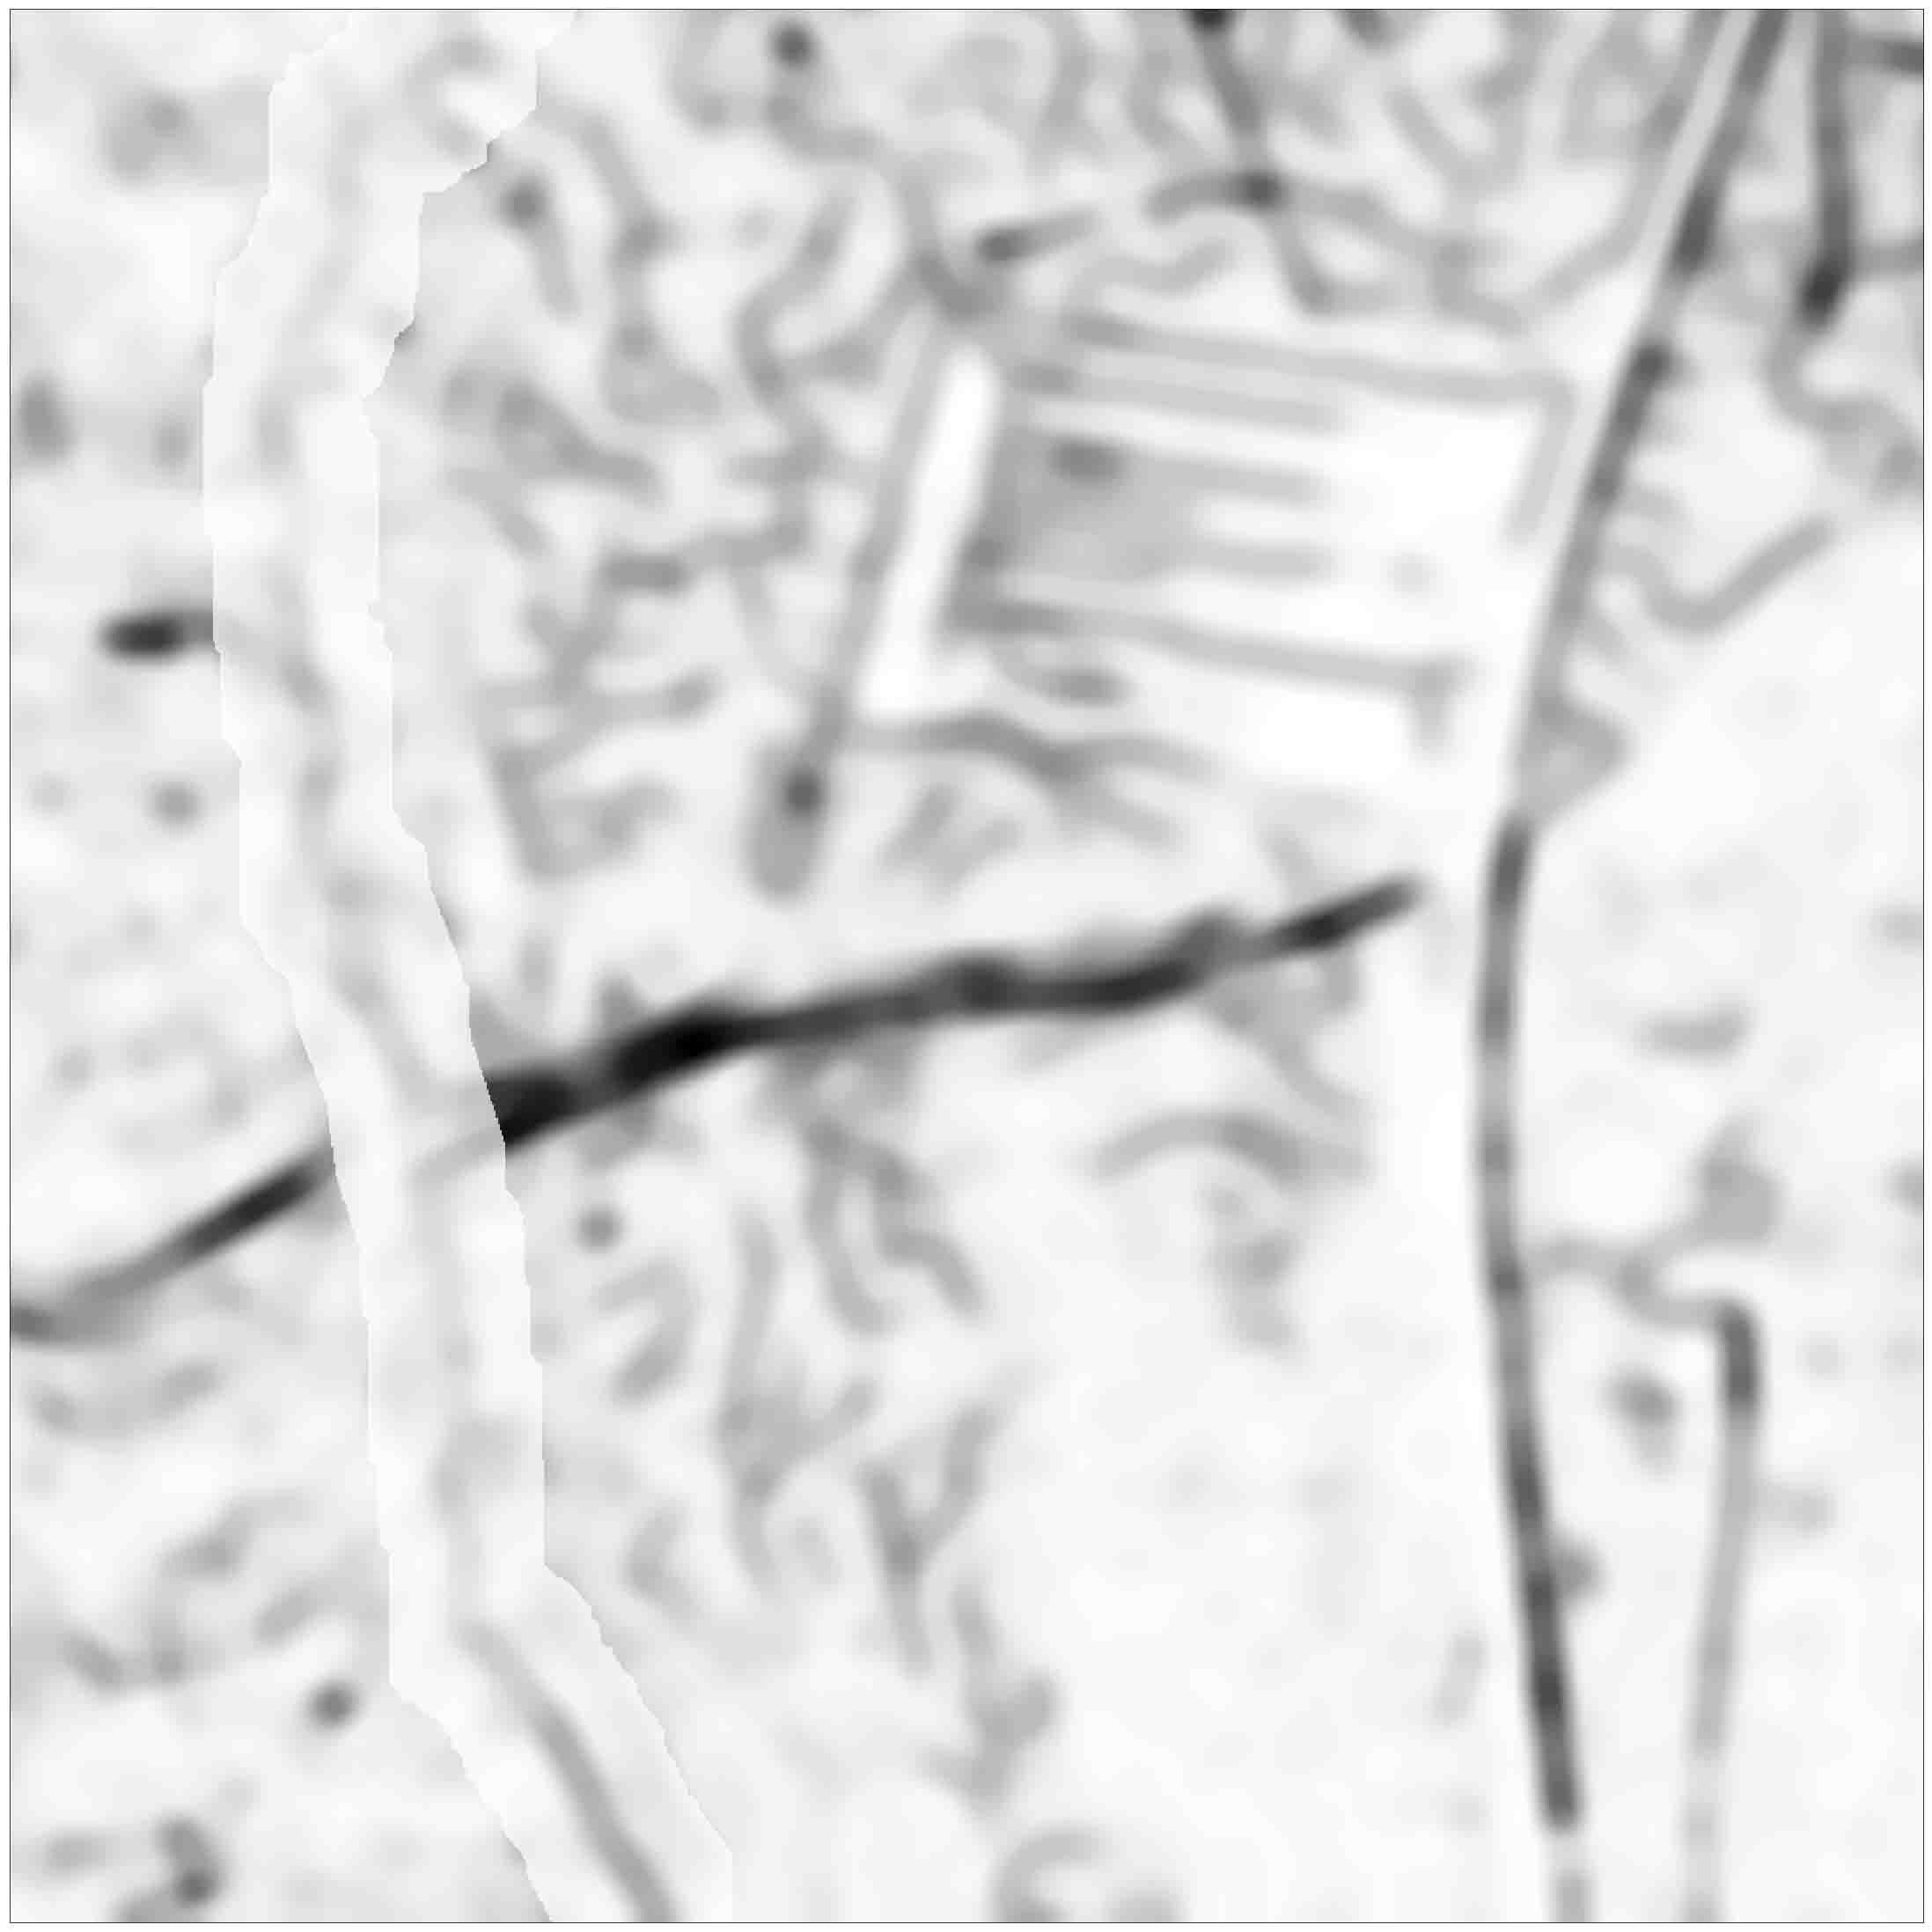
\includegraphics{./images/feature_l_lo.jpg}}}%%%
\DIFdelFL{\hspace{5pt}
    }\DIFdelendFL \caption{Example of \DIFdelbeginFL \DIFdelFL{11 }\DIFdelendFL \DIFaddbeginFL \DIFaddFL{8 }\DIFaddendFL of the \DIFdelbeginFL \DIFdelFL{81 }\DIFdelendFL \DIFaddbeginFL \DIFaddFL{40 }\DIFaddendFL input variables, in addition to ditch labels used by the \DIFdelbeginFL \DIFdelFL{model }\DIFdelendFL \DIFaddbeginFL \DIFaddFL{models }\DIFaddendFL for a small sample area. The radii represents pixels with a 0.5 m resolution. \newline \textbf{a:} Labelled ditches, \textbf{b:} Slope standard deviation, radius 6, \textbf{c:} HPMF mean, radius 4, \textbf{d:} HPMF \DIFdelbeginFL \DIFdelFL{Gabor, }\textbf{\DIFdelFL{e:}} %DIFAUXCMD
\DIFdelFL{HPMF }\DIFdelendFL ditch amplification, \DIFdelbeginFL \textbf{\DIFdelFL{f:}} %DIFAUXCMD
\DIFdelFL{HPMF ditch amplification - streams removed }\textbf{\DIFdelFL{g:}} %DIFAUXCMD
\DIFdelendFL \DIFaddbeginFL \textbf{\DIFaddFL{e:}} \DIFaddendFL Sky View Factor Gabor, \DIFdelbeginFL \textbf{\DIFdelFL{h:}} %DIFAUXCMD
\DIFdelendFL \DIFaddbeginFL \textbf{\DIFaddFL{f:}} \DIFaddendFL Sky View Factor max, radius 6, \DIFdelbeginFL \textbf{\DIFdelFL{i:}} %DIFAUXCMD
\DIFdelFL{Sky View Factor non-ditch amplification  }\textbf{\DIFdelFL{j:}} %DIFAUXCMD
\DIFdelendFL \DIFaddbeginFL \textbf{\DIFaddFL{g:}} \DIFaddendFL Impoundment mean, radius 3, \DIFdelbeginFL \textbf{\DIFdelFL{k:}} %DIFAUXCMD
\DIFdelendFL \DIFaddbeginFL \textbf{\DIFaddFL{h:}} \DIFaddendFL Impoundment ditch amplification, \DIFdelbeginFL \textbf{\DIFdelFL{l:}} %DIFAUXCMD
\DIFdelendFL \DIFaddbeginFL \textbf{\DIFaddFL{i:}} \DIFaddendFL Impoundment ditch amplification - streams removed}
    \label{fig:features}
\end{figure}
\DIFdelbegin %DIFDELCMD < \clearpage
%DIFDELCMD < %%%
\DIFdelend 

\subsubsection{Training and validation datasets}
\label{trainingvalidationdatasets}
To develop and evaluate our \DIFdelbegin \DIFdel{model}\DIFdelend \DIFaddbegin \DIFadd{ditch detector}\DIFaddend , the raster and ditch label data of Krycklan were manually divided into 21 subsections. Each subsection represents an area of roughly 196 hectare. From this division, 11 of the subsections were put aside as hold-out data, only for use in the experiment to evaluate the performance of the predictions. The remaining 10 subsections were used solely before the experiment to develop the \DIFdelbegin \DIFdel{model }\DIFdelend \DIFaddbegin \DIFadd{ditch detector }\DIFaddend to test different ways of preparing the data. This allowed the \DIFdelbegin \DIFdel{model }\DIFdelend \DIFaddbegin \DIFadd{ditch detector }\DIFaddend to be evaluated on  \DIFdelbegin \DIFdel{unseen data to strengthen }\DIFdelend \DIFaddbegin \DIFadd{independent data and  strengthened }\DIFaddend the validity of the experiment. \hyperref[fig:swedenkrycklan]{Figure} \ref{fig:swedenkrycklan} shows which subsections were used for development and evaluation respectively.

Using the 11 subsections in the hold-out data for the final experiment, a process called \textit{k-fold cross validation} was employed (11-fold cross validation in our case). K-fold cross validation is a method where you divide your dataset into folds of similar size and train a model on all but one of your folds (subsections). You then use that subsection to evaluate the results \citep{crossvalidation}. \DIFaddbegin \DIFadd{A new model is trained using the training folds for each iteration (}\hyperref[fig:crossvalidation]{Figure} \DIFadd{\ref{fig:crossvalidation}). }\DIFaddend Using this technique, shifting which subsection to leave out from the training, allowed us to train 11 different Random Forests classifying models with a large amount of data from the remaining 10 subsections in the hold-out data, producing 11 \DIFaddbegin \DIFadd{independent }\DIFaddend sub-experiments to evaluate the method on.

\DIFdelbegin \subsection{\DIFdel{Building the Random Forests model}}
%DIFAUXCMD
\addtocounter{subsection}{-1}%DIFAUXCMD
\DIFdelend \DIFaddbegin \begin{figure}[!htb]
    \centering
    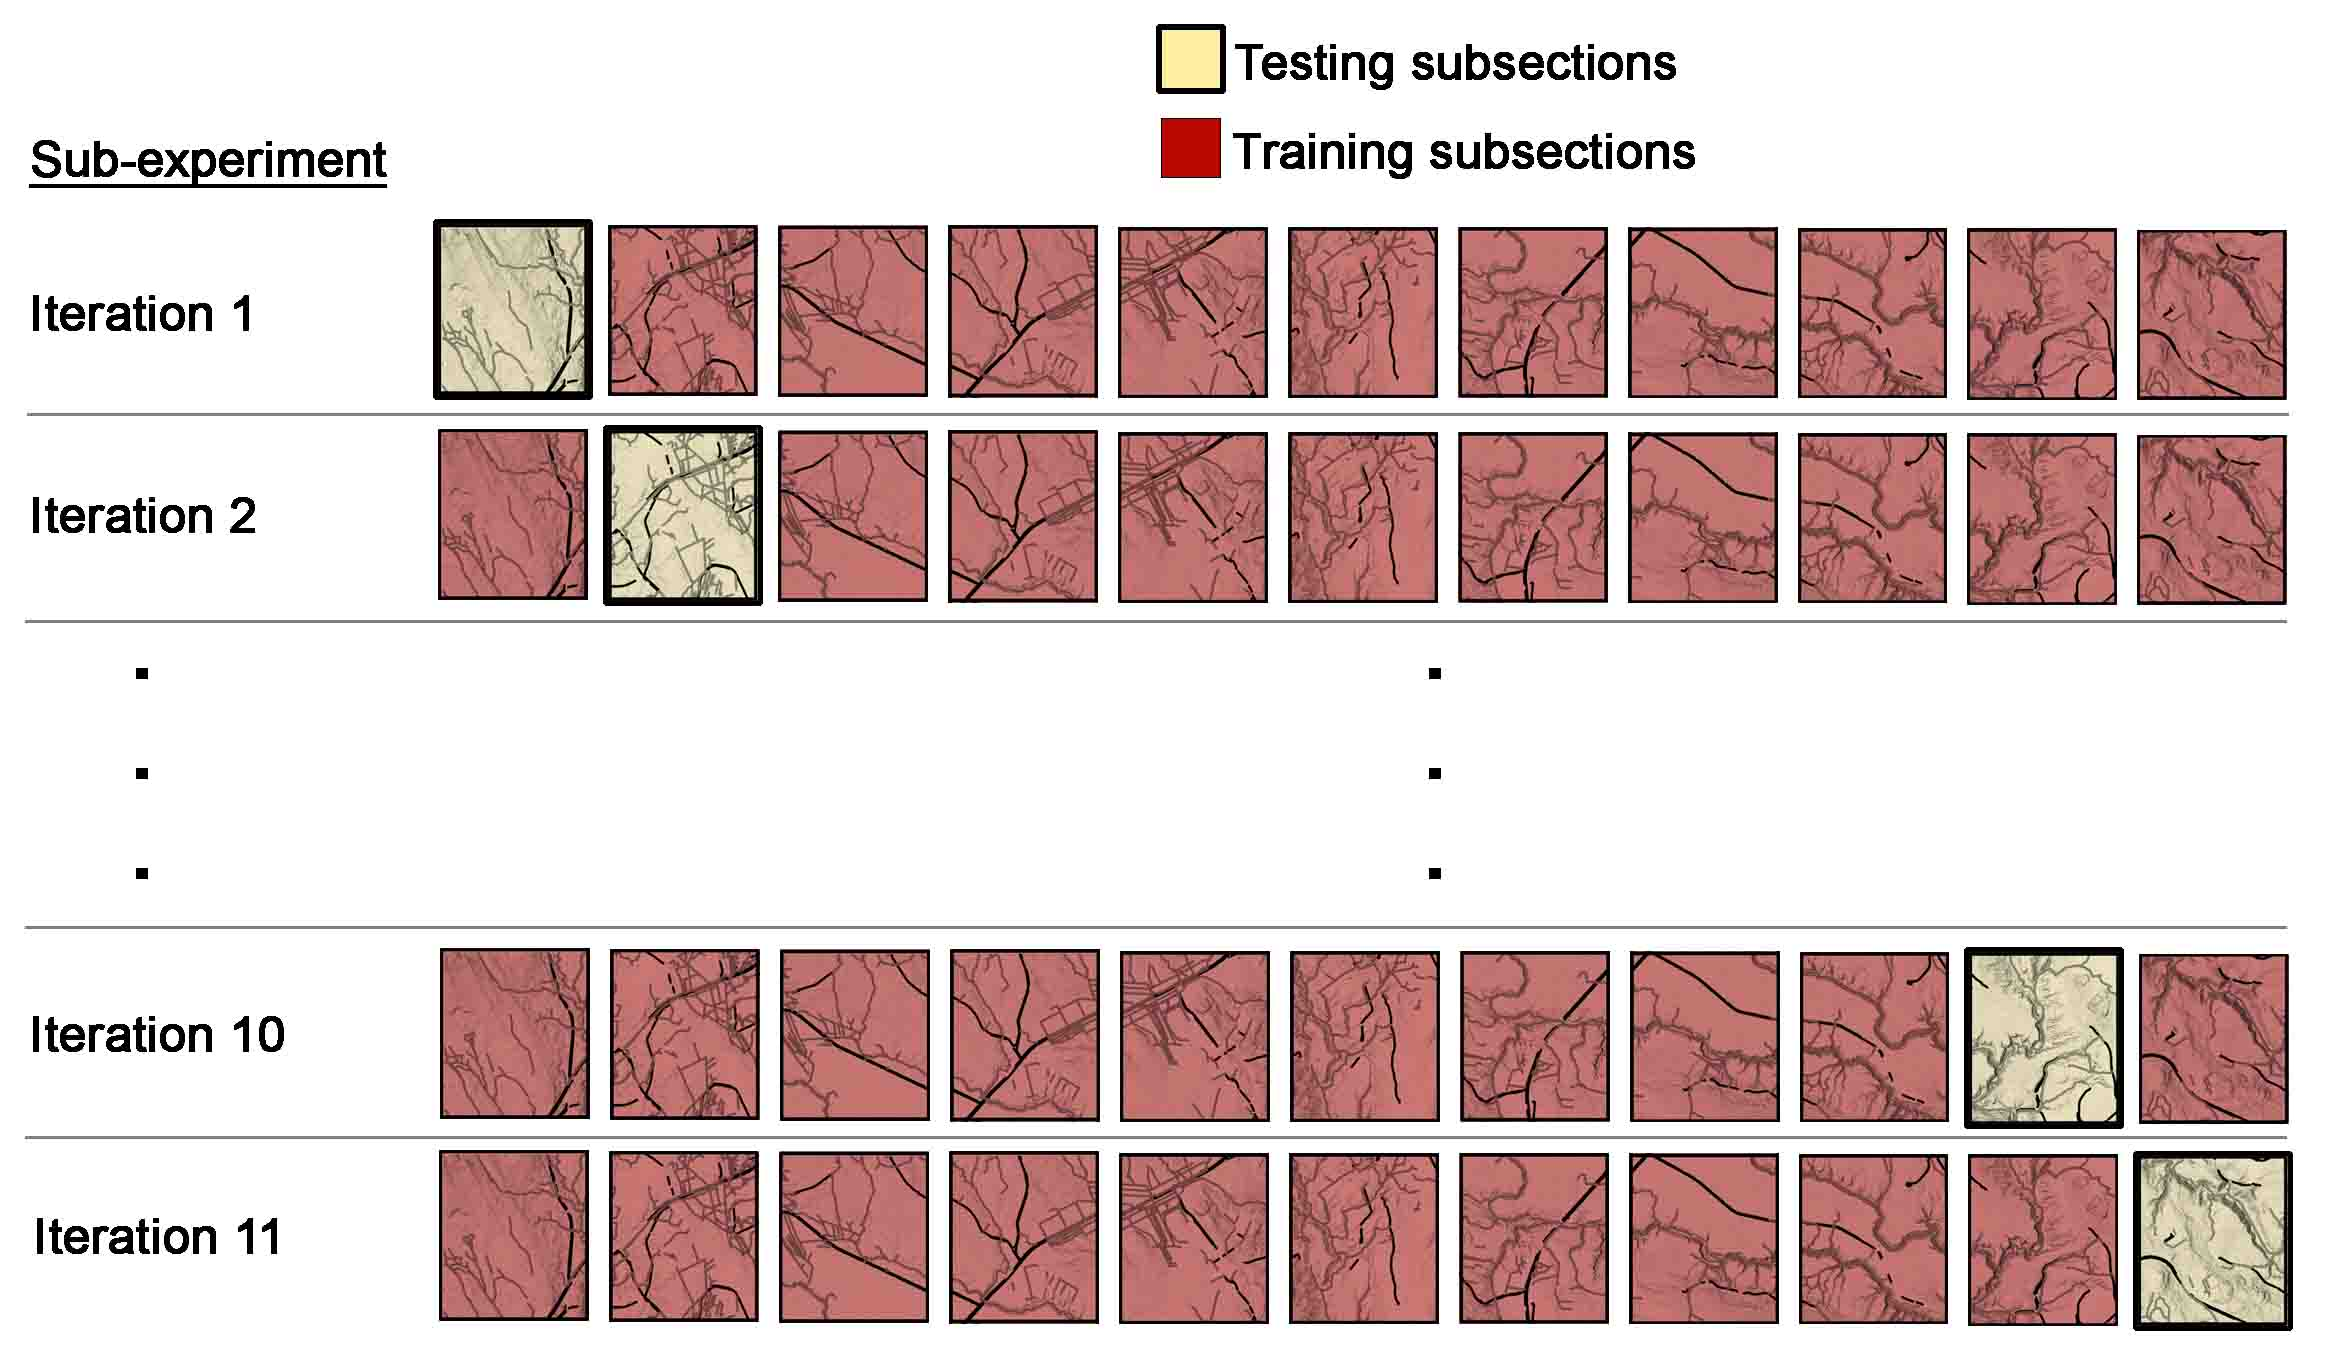
\includegraphics[width=1\linewidth]{images/cross_validation_lo.jpg}
    \caption{\DIFaddFL{11-fold cross validation. Each subsection in the hold-out data was used once for testing, with the remaining subsections being used to build a new model for each iteration.}}
    \label{fig:crossvalidation}
\end{figure}
\DIFaddend 

\DIFdelbegin \textit{\DIFdel{Model ensembles}} %DIFAUXCMD
\DIFdel{is a category of machine learning where a set of models can be combined to increase diversity and robustness of predictions \mbox{%DIFAUXCMD
\citep{flach}}\hspace{0pt}%DIFAUXCMD
. Random Forests is a supervised learning algorithm, first developed by \mbox{%DIFAUXCMD
\citet{breiman}}\hspace{0pt}%DIFAUXCMD
, that makes use of the model ensemble technique by using a set of decision trees to build a }\textit{\DIFdel{forest}} %DIFAUXCMD
\DIFdel{of trees. The outputs from these trees are then examined, and a class probability estimation ranging from 0 to 1 can be produced for each sample by dividing the amount of tree outputs of a class with the total amount of trees \mbox{%DIFAUXCMD
\citep{breiman}}\hspace{0pt}%DIFAUXCMD
.
}\DIFdelend \DIFaddbegin \subsection{\DIFadd{Developing the Random Forests model}}
\DIFaddend 

\DIFdelbegin \DIFdel{The decision tree data structure is a }\textit{\DIFdel{tree}} %DIFAUXCMD
\DIFdel{of connected nodes where the end node of each branch (leaf) produces an output value. Each step in the tree aims to minimise the entropy of the outputs \mbox{%DIFAUXCMD
\citep{kotsiantis}}\hspace{0pt}%DIFAUXCMD
. Each node in a decision tree represents a variable or an abstraction of variables from the inputs and each split is made by using this variable to separate the inputs.
}%DIFDELCMD < 

%DIFDELCMD < %%%
\DIFdel{Random Forests uses two techniques called }\textit{\DIFdel{subspace sampling}} %DIFAUXCMD
\DIFdel{and }\textit{\DIFdel{bootstrap aggregation}} %DIFAUXCMD
\DIFdel{(bagging) in tandem \mbox{%DIFAUXCMD
\citep{breiman}}\hspace{0pt}%DIFAUXCMD
. Subspace sampling is the process of drawing a random subset of variables from the input variable set \mbox{%DIFAUXCMD
\citet{ho}}\hspace{0pt}%DIFAUXCMD
. The bagging technique takes, with replacement, a set of different random samples for constructing each tree \mbox{%DIFAUXCMD
\citep{flach}}\hspace{0pt}%DIFAUXCMD
. There are several hyperparameters that can be tuned to achieve better results from the model. For example, you can adjust the amount of decision trees to use, or the maximum amount of input variables to use for each subspace sampling \mbox{%DIFAUXCMD
\citep{scikit-learn}}\hspace{0pt}%DIFAUXCMD
. We performed a simple hyperparameter tuning to determine what parameter values for the Random Forests algorithm would yield the best prediction. Evaluating a maximum of 25 input variables for each node , and using 200 trees produced the best results. Setting the class weight to }\textit{\DIFdel{balanced}} %DIFAUXCMD
\DIFdel{also improved the performance of the classifier.
}%DIFDELCMD < 

%DIFDELCMD < \newpage
%DIFDELCMD < 

%DIFDELCMD < %%%
\DIFdel{Random Forests computes Gini importance, which shows how often a variable is selected for a split for a certain classification \mbox{%DIFAUXCMD
\citep{gini}}\hspace{0pt}%DIFAUXCMD
. Each input variable is given a Gini impurity rating, which measures the frequency of incorrect labelling occurring from its use. As the Gini impurity rating for a variable increases, its Gini importance decreases \mbox{%DIFAUXCMD
\citep{gini}}\hspace{0pt}%DIFAUXCMD
. When the model is trained, it examines the Gini importance from all trees and produces the total Gini importance as a value between 0 and 1 \mbox{%DIFAUXCMD
\citep{gini}}\hspace{0pt}%DIFAUXCMD
. The Gini importance can help when developing a model by indirectly giving advice on new input variables to introduce.
}%DIFDELCMD < 

%DIFDELCMD < %%%
\DIFdelend \DIFaddbegin \DIFadd{Random Forests is an ensemble machine learning method which builds multiple diverse decision trees to increase the robustness of its predictions \mbox{%DIFAUXCMD
\citep{breiman,flach}}\hspace{0pt}%DIFAUXCMD
. }\DIFaddend The \DIFaddbegin \DIFadd{individual trees are trained by minimising the entropy of the data from each nodeÔÇÖs output \mbox{%DIFAUXCMD
\citep{kotsiantis}}\hspace{0pt}%DIFAUXCMD
. A byproduct of the training is the Gini importance, which denotes the most important input variables \mbox{%DIFAUXCMD
\citep{gini}}\hspace{0pt}%DIFAUXCMD
. For our study, a hyperparameter tuning showed that using 300 trees and }\textit{\DIFadd{gini}} \DIFadd{as the splitting criterion, with a minimum of 10 samples per node split, and no artificial class weight or max depth of trees yielded the best predictions. The }\DIFaddend Random Forests algorithm from the \DIFdelbegin \DIFdel{python }\DIFdelend \DIFaddbegin \DIFadd{Python }\DIFaddend library \textit{scikit-learn} \DIFaddbegin \DIFadd{\mbox{%DIFAUXCMD
\citep{scikit-learn} }\hspace{0pt}%DIFAUXCMD
}\DIFaddend was used in the experiment, and the \DIFdelbegin \DIFdel{classifier was }\DIFdelend \DIFaddbegin \DIFadd{classifiers were }\DIFaddend trained on all the input variables seen in \hyperref[featuretable]{Table} \ref{featuretable}.
\DIFdelbegin \DIFdel{The probability predictions used in this Random Forests implementation are computed by counting the number of occurrences of a class output and dividing with the total amount of trees in the forest \mbox{%DIFAUXCMD
\citep{scikit-learn}}\hspace{0pt}%DIFAUXCMD
. The testing phase showed that the classifier produced poor results when the ratio of ditch- versus non-ditch pixels in the training data was very high. A high ratio led to the model not being punished for mislabelling ditches as non-ditches, causing it to prioritise a high accuracy over a high recall. According to \mbox{%DIFAUXCMD
\citet{balanced}}\hspace{0pt}%DIFAUXCMD
, an imbalanced training dataset causes a minority class to be less accurately predicted. Because the ditch class is much less common than the non-ditch class, we attempted to train the model with a roughly equal amount of ditch pixels and non-ditch pixels to balance the model. The model was, however, still evaluated on all the pixels in the 11 validation subsections.
}\DIFdelend 

\begin{table} [!htb]
    \DIFdelbeginFL %DIFDELCMD < \tbl{The 81 input variables used when training the model.}
%DIFDELCMD <     %%%
\DIFdelendFL \DIFaddbeginFL \caption{The 40 input variables used when training the models.}
    \DIFaddendFL {\begin{tabular}{ll} \toprule
      Variable/Algorithm\textsuperscript{a} & Circular radii\textsuperscript{b} \\ \midrule

      Sky View Factor \DIFdelbeginFL \DIFdelFL{raw }%DIFDELCMD < & %%%
\DIFdelFL{-}%DIFDELCMD < \\
%DIFDELCMD <       %%%
\DIFdelFL{Sky View Factor mean }%DIFDELCMD < & %%%
\DIFdelFL{2, 3, 4, 6 }%DIFDELCMD < \\
%DIFDELCMD <       %%%
\DIFdelFL{Sky View Factor }\DIFdelendFL median &2, \DIFdelbeginFL \DIFdelFL{4, }\DIFdelendFL 6 \\
      Sky View Factor standard deviation & \DIFdelbeginFL \DIFdelFL{2, 4, }\DIFdelendFL 6 \\
      Sky View Factor min & \DIFdelbeginFL \DIFdelFL{2, 4, }\DIFdelendFL 6 \\
      Sky View Factor max & 2, 4, 6 \\
      Sky View Factor non ditch amplification & - \\ 
      Sky View Factor \DIFdelbeginFL \DIFdelFL{conic filter - streams removed }%DIFDELCMD < & %%%
\DIFdelFL{- }%DIFDELCMD < \\ 
%DIFDELCMD <       %%%
\DIFdelFL{Sky View Factor }\DIFdelendFL Gabor & - \\
      Sky View Factor Gabor - streams removed & -\\

      Impoundment \DIFdelbeginFL \DIFdelFL{raw }%DIFDELCMD < & %%%
\DIFdelFL{- }%DIFDELCMD < \\
%DIFDELCMD <       %%%
\DIFdelFL{Impoundment }\DIFdelendFL mean & 2, 3, 4, 6 \\
      Impoundment median & 2, 4, 6 \\
      Impoundment standard deviation & \DIFdelbeginFL \DIFdelFL{2, }\DIFdelendFL 4, 6 \\
      Impoundment \DIFdelbeginFL \DIFdelFL{min }%DIFDELCMD < & %%%
\DIFdelFL{2, 4, 6 }%DIFDELCMD < \\
%DIFDELCMD <       %%%
\DIFdelFL{Impoundment }\DIFdelendFL max & \DIFdelbeginFL \DIFdelFL{2, 4, }\DIFdelendFL 6 \\
      Impoundment ditch amplification & - \\
      Impoundment ditch amplification - streams removed & - \\

      HPMF \DIFdelbeginFL \DIFdelFL{raw }%DIFDELCMD < & %%%
\DIFdelFL{- }%DIFDELCMD < \\
%DIFDELCMD <       %%%
\DIFdelFL{HPMF }\DIFdelendFL mean & \DIFdelbeginFL \DIFdelFL{2, }\DIFdelendFL 3, 4, 6 \\
      HPMF median & \DIFdelbeginFL \DIFdelFL{2, }\DIFdelendFL 4 \DIFdelbeginFL \DIFdelFL{, 6 }\DIFdelendFL \\
      HPMF standard deviation & \DIFdelbeginFL \DIFdelFL{2, 4, }\DIFdelendFL 6 \\
      HPMF min & 2, 4 \DIFdelbeginFL \DIFdelFL{, 6 }\DIFdelendFL \\
      HPMF \DIFdelbeginFL \DIFdelFL{max }%DIFDELCMD < & %%%
\DIFdelFL{2, 4, 6 }%DIFDELCMD < \\
%DIFDELCMD <       %%%
\DIFdelFL{HPMF }\DIFdelendFL ditch amplification & - \\
      HPMF ditch amplification - streams removed & - \\
      HPMF Gabor \DIFdelbeginFL %DIFDELCMD < & %%%
\DIFdelendFL - \DIFdelbeginFL %DIFDELCMD < \\
%DIFDELCMD <       %%%
\DIFdelFL{HPMF Gabor - }\DIFdelendFL streams removed & -\\

      Slope \DIFdelbeginFL \DIFdelFL{raw }%DIFDELCMD < & %%%
\DIFdelFL{- }%DIFDELCMD < \\
%DIFDELCMD <       %%%
\DIFdelFL{Slope }\DIFdelendFL mean & \DIFdelbeginFL \DIFdelFL{2, 3, 4, }\DIFdelendFL 6 \\
      Slope median & \DIFdelbeginFL \DIFdelFL{2, 4, }\DIFdelendFL 6 \\
      Slope standard deviation & \DIFdelbeginFL \DIFdelFL{2, }\DIFdelendFL 4, 6 \\
      Slope min & 2, 4, 6 \\
      Slope \DIFdelbeginFL \DIFdelFL{max }%DIFDELCMD < & %%%
\DIFdelFL{2, 4, 6 }%DIFDELCMD < \\
%DIFDELCMD <       %%%
\DIFdelFL{Slope }\DIFdelendFL non-ditch amplification & - \\ \bottomrule
    \end{tabular}}
    \tabnote{\textsuperscript{a} Displays algorithm used to produce the variable. \newline
        \textsuperscript{b} Represents the radius of the circular mask (if one was used) to determine \newline what neighbouring pixels to use in an algorithm. The radii represents pixels \newline \mbox{with a 0.5 m resolution.\itshape\ignorespaces}}
    \label{featuretable}
\end{table}

The \DIFdelbegin \DIFdel{first step to create a more balanced training dataset was to extract }\DIFdelend \DIFaddbegin \DIFadd{testing phase showed that the classifiers produced poor results when the ratio of ditch versus non-ditch pixels in the training data was very high, as the models were not being punished for mislabelling ditches as non-ditches. To increase the recall, we evened out the amount of ditch and non-ditch instances in the training data. First, we extracted }\DIFaddend all pixels labelled as ditches \DIFdelbegin \DIFdel{, }\DIFdelend as well as pixels within close proximity of ditches. Secondly, pixels were sampled randomly from the entire subsection \DIFdelbegin \DIFdel{. This allowed the training dataset to be fairly balanced while still containing }\DIFdelend \DIFaddbegin \DIFadd{to still contain }\DIFaddend most of the geographical features of each \DIFdelbegin \DIFdel{subsection }\DIFdelend \DIFaddbegin \DIFadd{area }\DIFaddend (\hyperref[fig:balancedmasks]{Figure} \ref{fig:balancedmasks}).

\begin{figure} [!htb]
    \centering
    \subfigure[]{
        \resizebox*{6.85cm}{!}{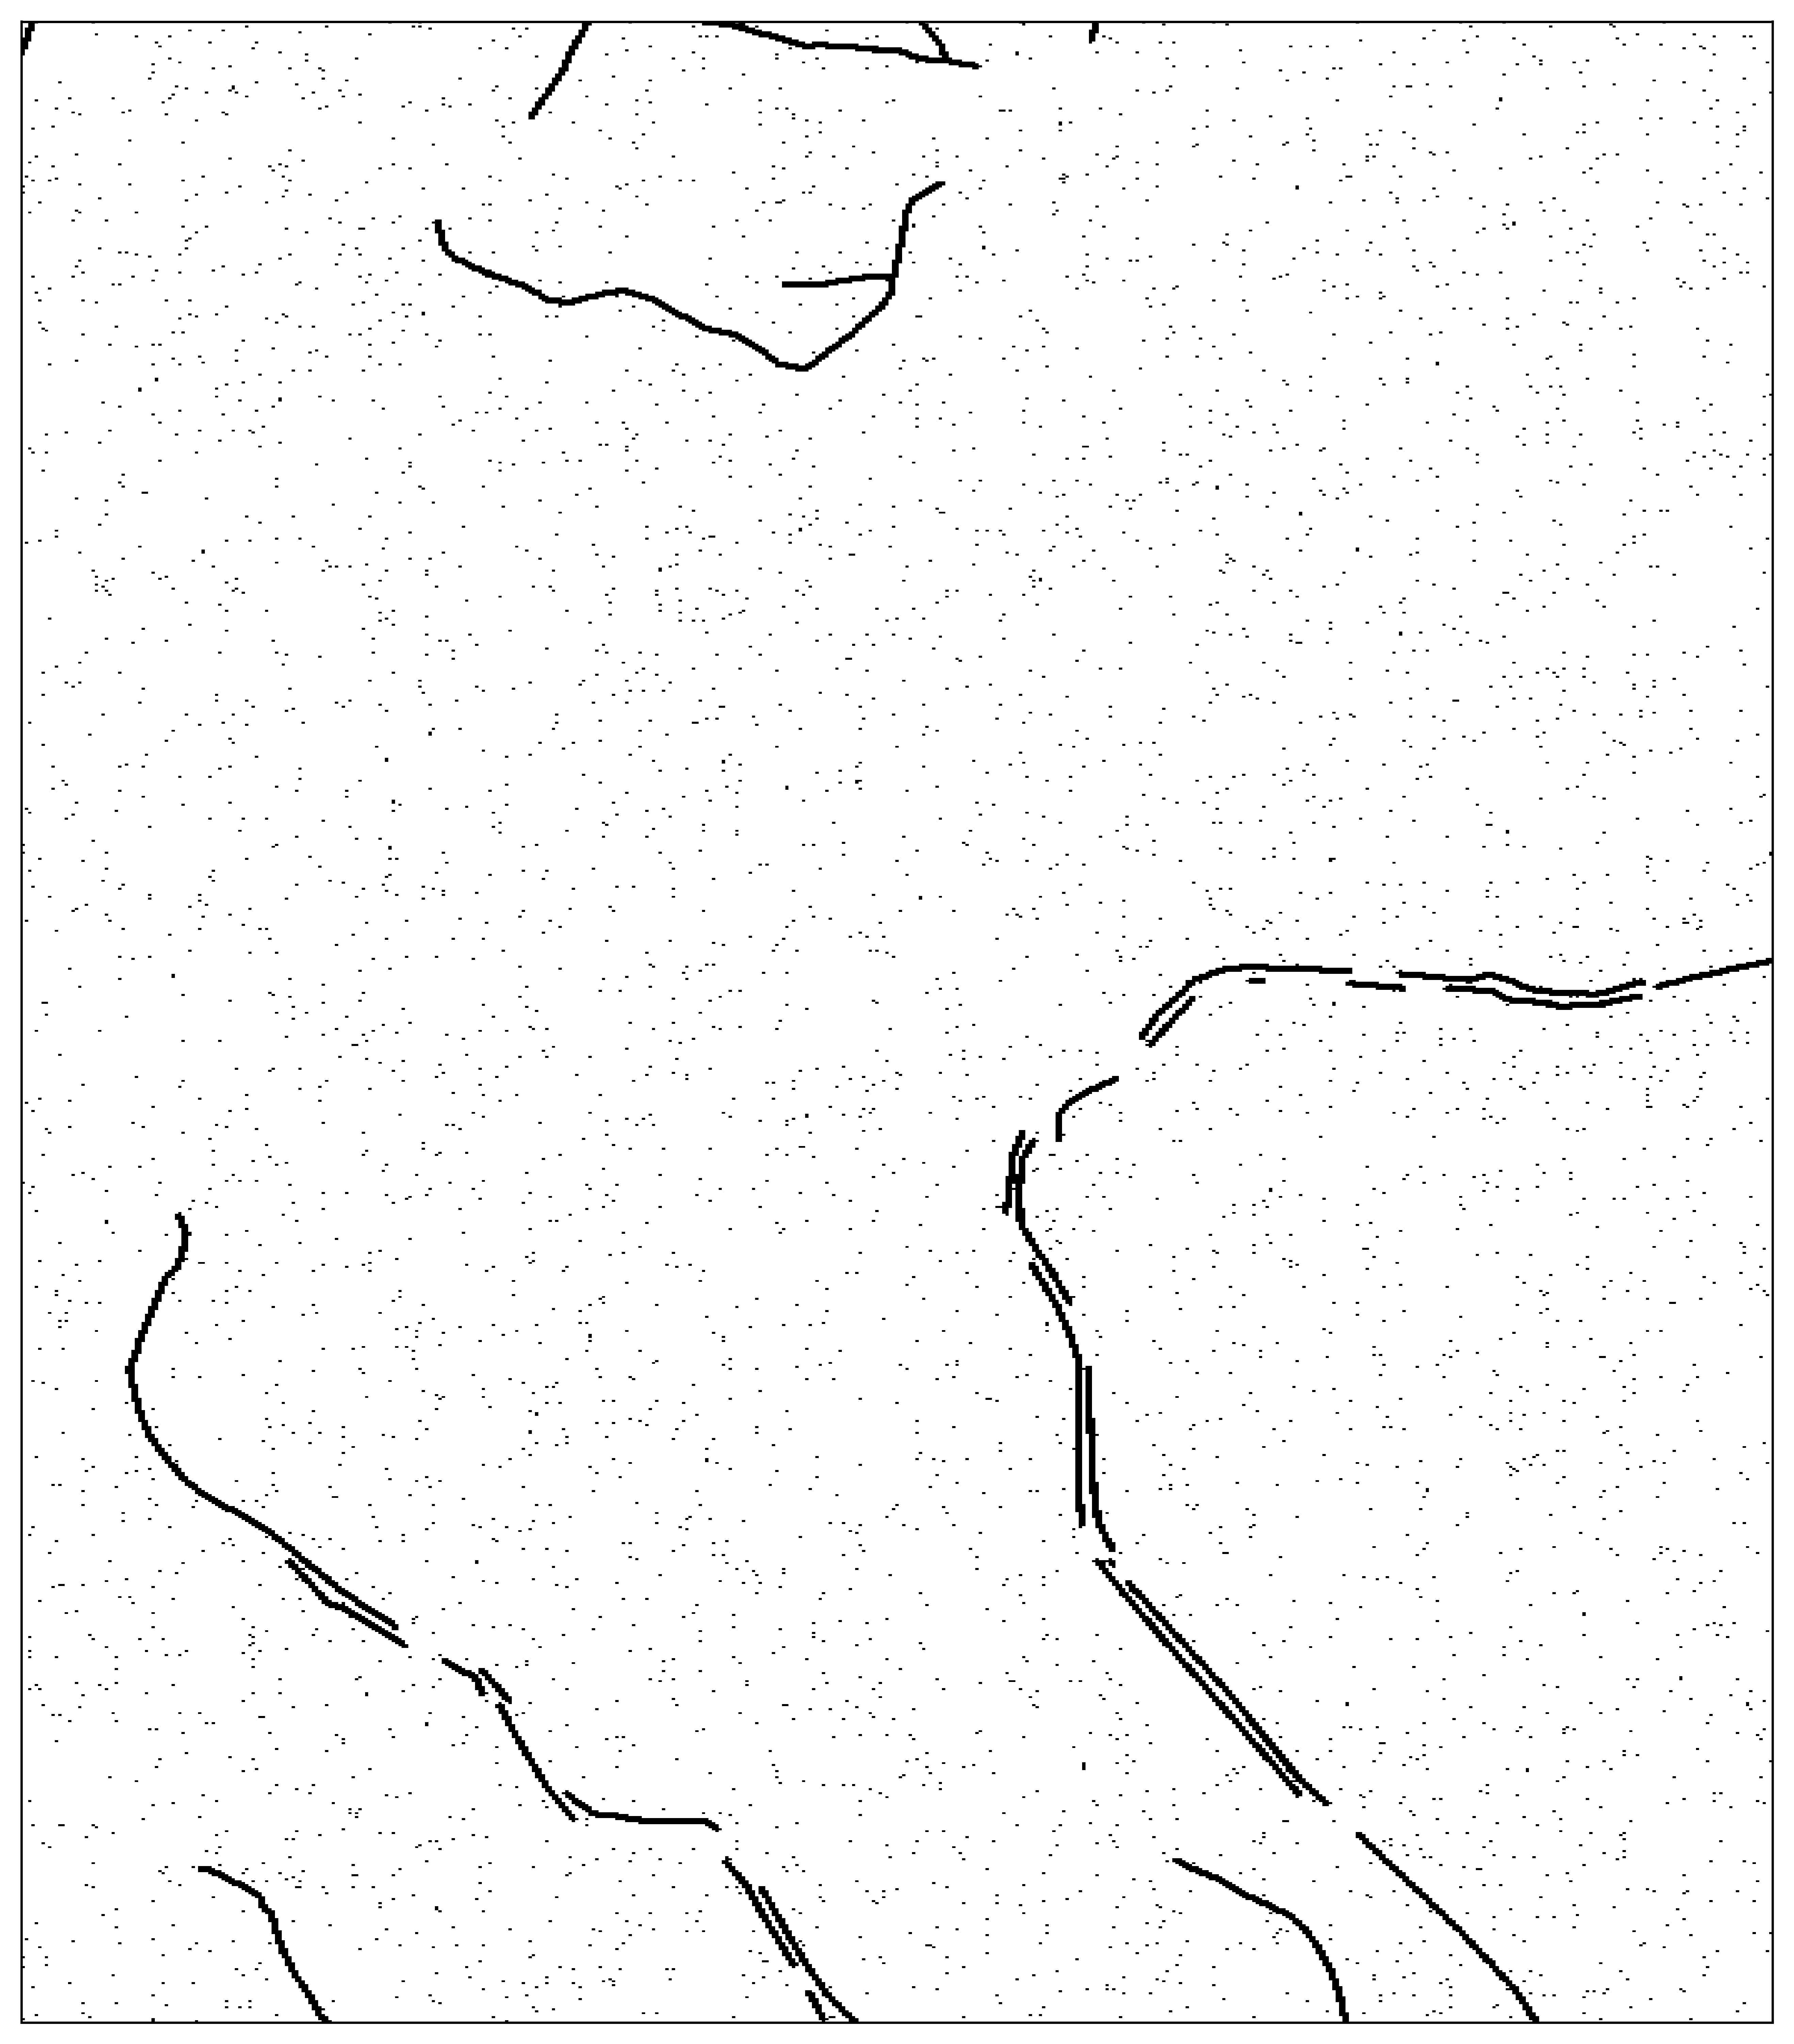
\includegraphics{./images/publ_balanced_masks_A_lo.jpg}}}\hspace{5pt}
    \subfigure[]{
        \resizebox*{6.85cm}{!}{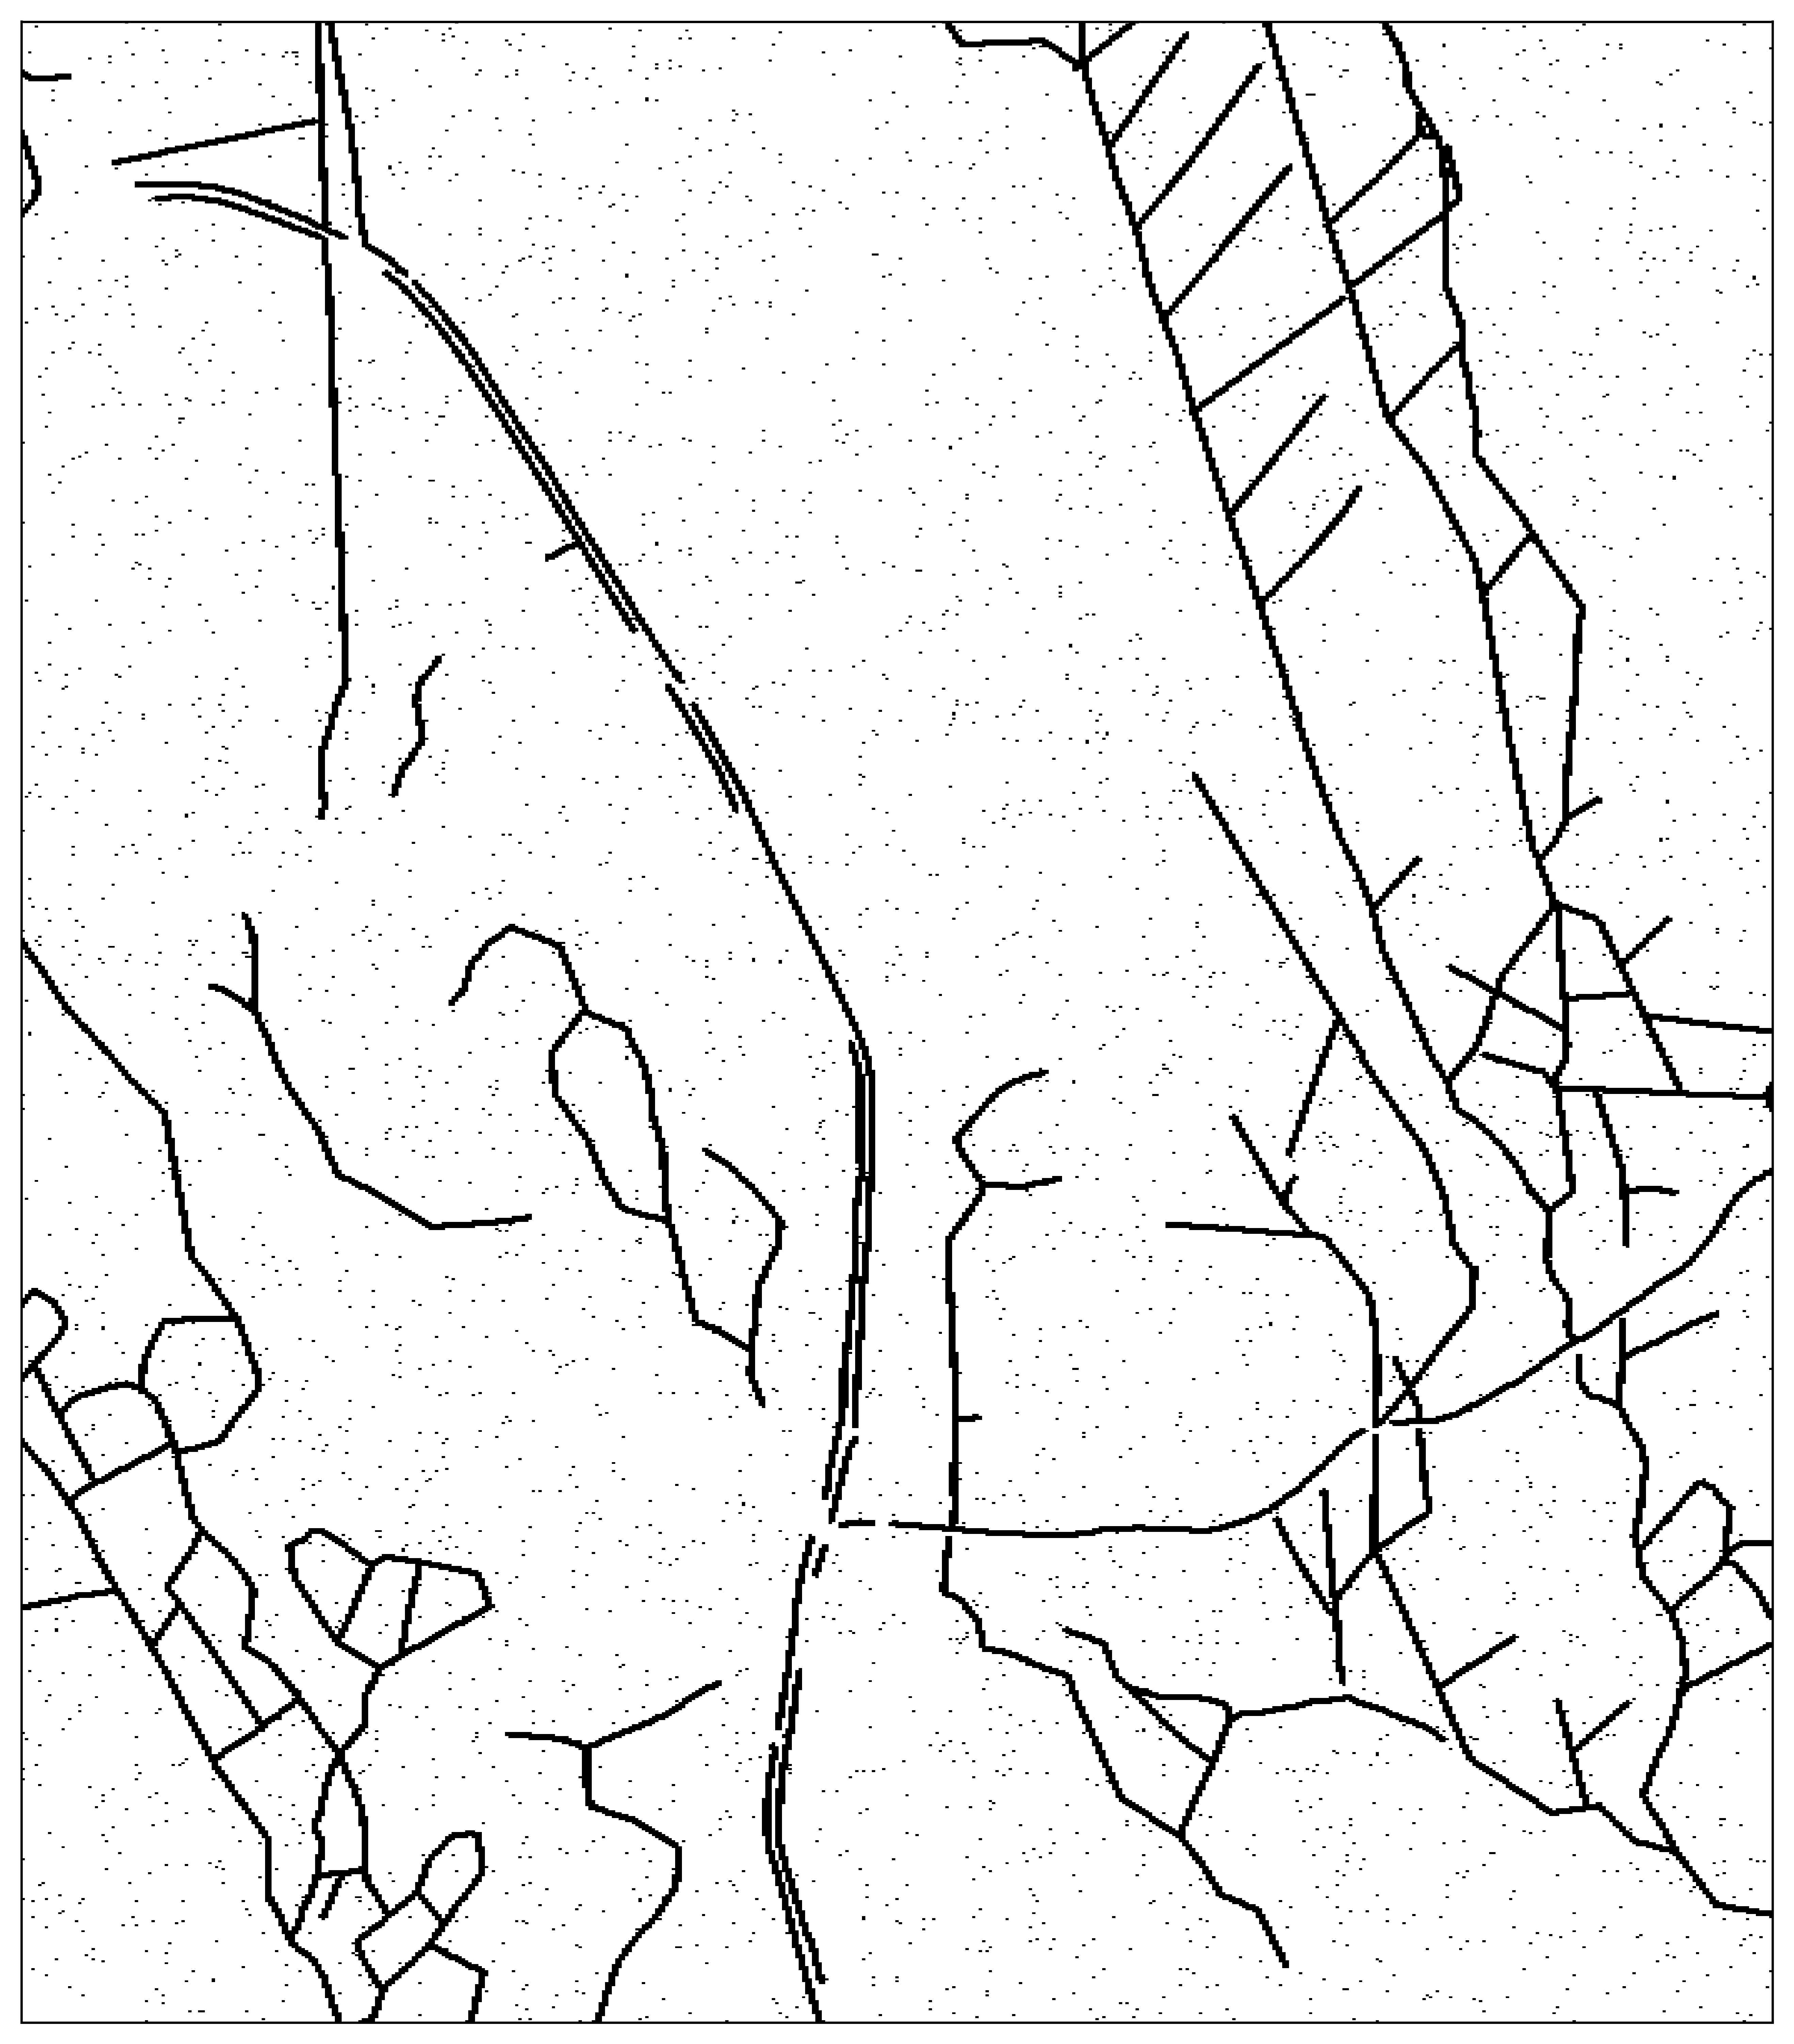
\includegraphics{./images/publ_balanced_masks_B_lo.jpg}}}
    \caption{Black pixels here indicate the balanced masks used to determine what pixels were used when training the \DIFdelbeginFL \DIFdelFL{model}\DIFdelendFL \DIFaddbeginFL \DIFaddFL{models}\DIFaddendFL . \textbf{a, b: }Examples of two subsection from the training dataset.}
    \label{fig:balancedmasks}
\end{figure}

\subsection{Post-processing}
The \DIFdelbegin \DIFdel{model outputs }\DIFdelend \DIFaddbegin \DIFadd{models output }\DIFaddend a ditch class probability prediction for each pixel. Values close to zero indicate a low probability of a pixel lying in a ditch, whereas values close to one equals a high ditch probability (\hyperref[fig:postprocessing1]{Figure} \ref{fig:postprocessing1} \hyperref[fig:postprocessing1]{a}).

\subsubsection{Noise reduction and gap filling}
\DIFaddbegin 

\DIFaddend The probability predictions contained a lot of noise in \DIFdelbegin \DIFdel{geographical locations far away from ditches, which needed to be excluded. The first step for removing noise was to use }\DIFdelend \DIFaddbegin \DIFadd{the areas largely distant from the ditches. This noise was removed by first using }\DIFaddend a bilateral de-noising filter\DIFdelbegin \DIFdel{on the entire prediction image}\DIFdelend \DIFaddbegin \DIFadd{, and then removing outlier pixels that were far away from any other high probability ditch pixels}\DIFaddend . This left linear properties and pixels with a very high value intact, while lowering the value of pixels that did not contribute to an accurate prediction (\hyperref[fig:postprocessing1]{Figure} \ref{fig:postprocessing1} \hyperref[fig:postprocessing1]{b}) \DIFdelbegin \DIFdel{.
}%DIFDELCMD < 

%DIFDELCMD < \begin{figure} [%%%
\DIFdelFL{!htb}%DIFDELCMD < ]
%DIFDELCMD <     \centering
%DIFDELCMD <     \subfigure[]{
%DIFDELCMD <         \resizebox*{6.85cm}{!}{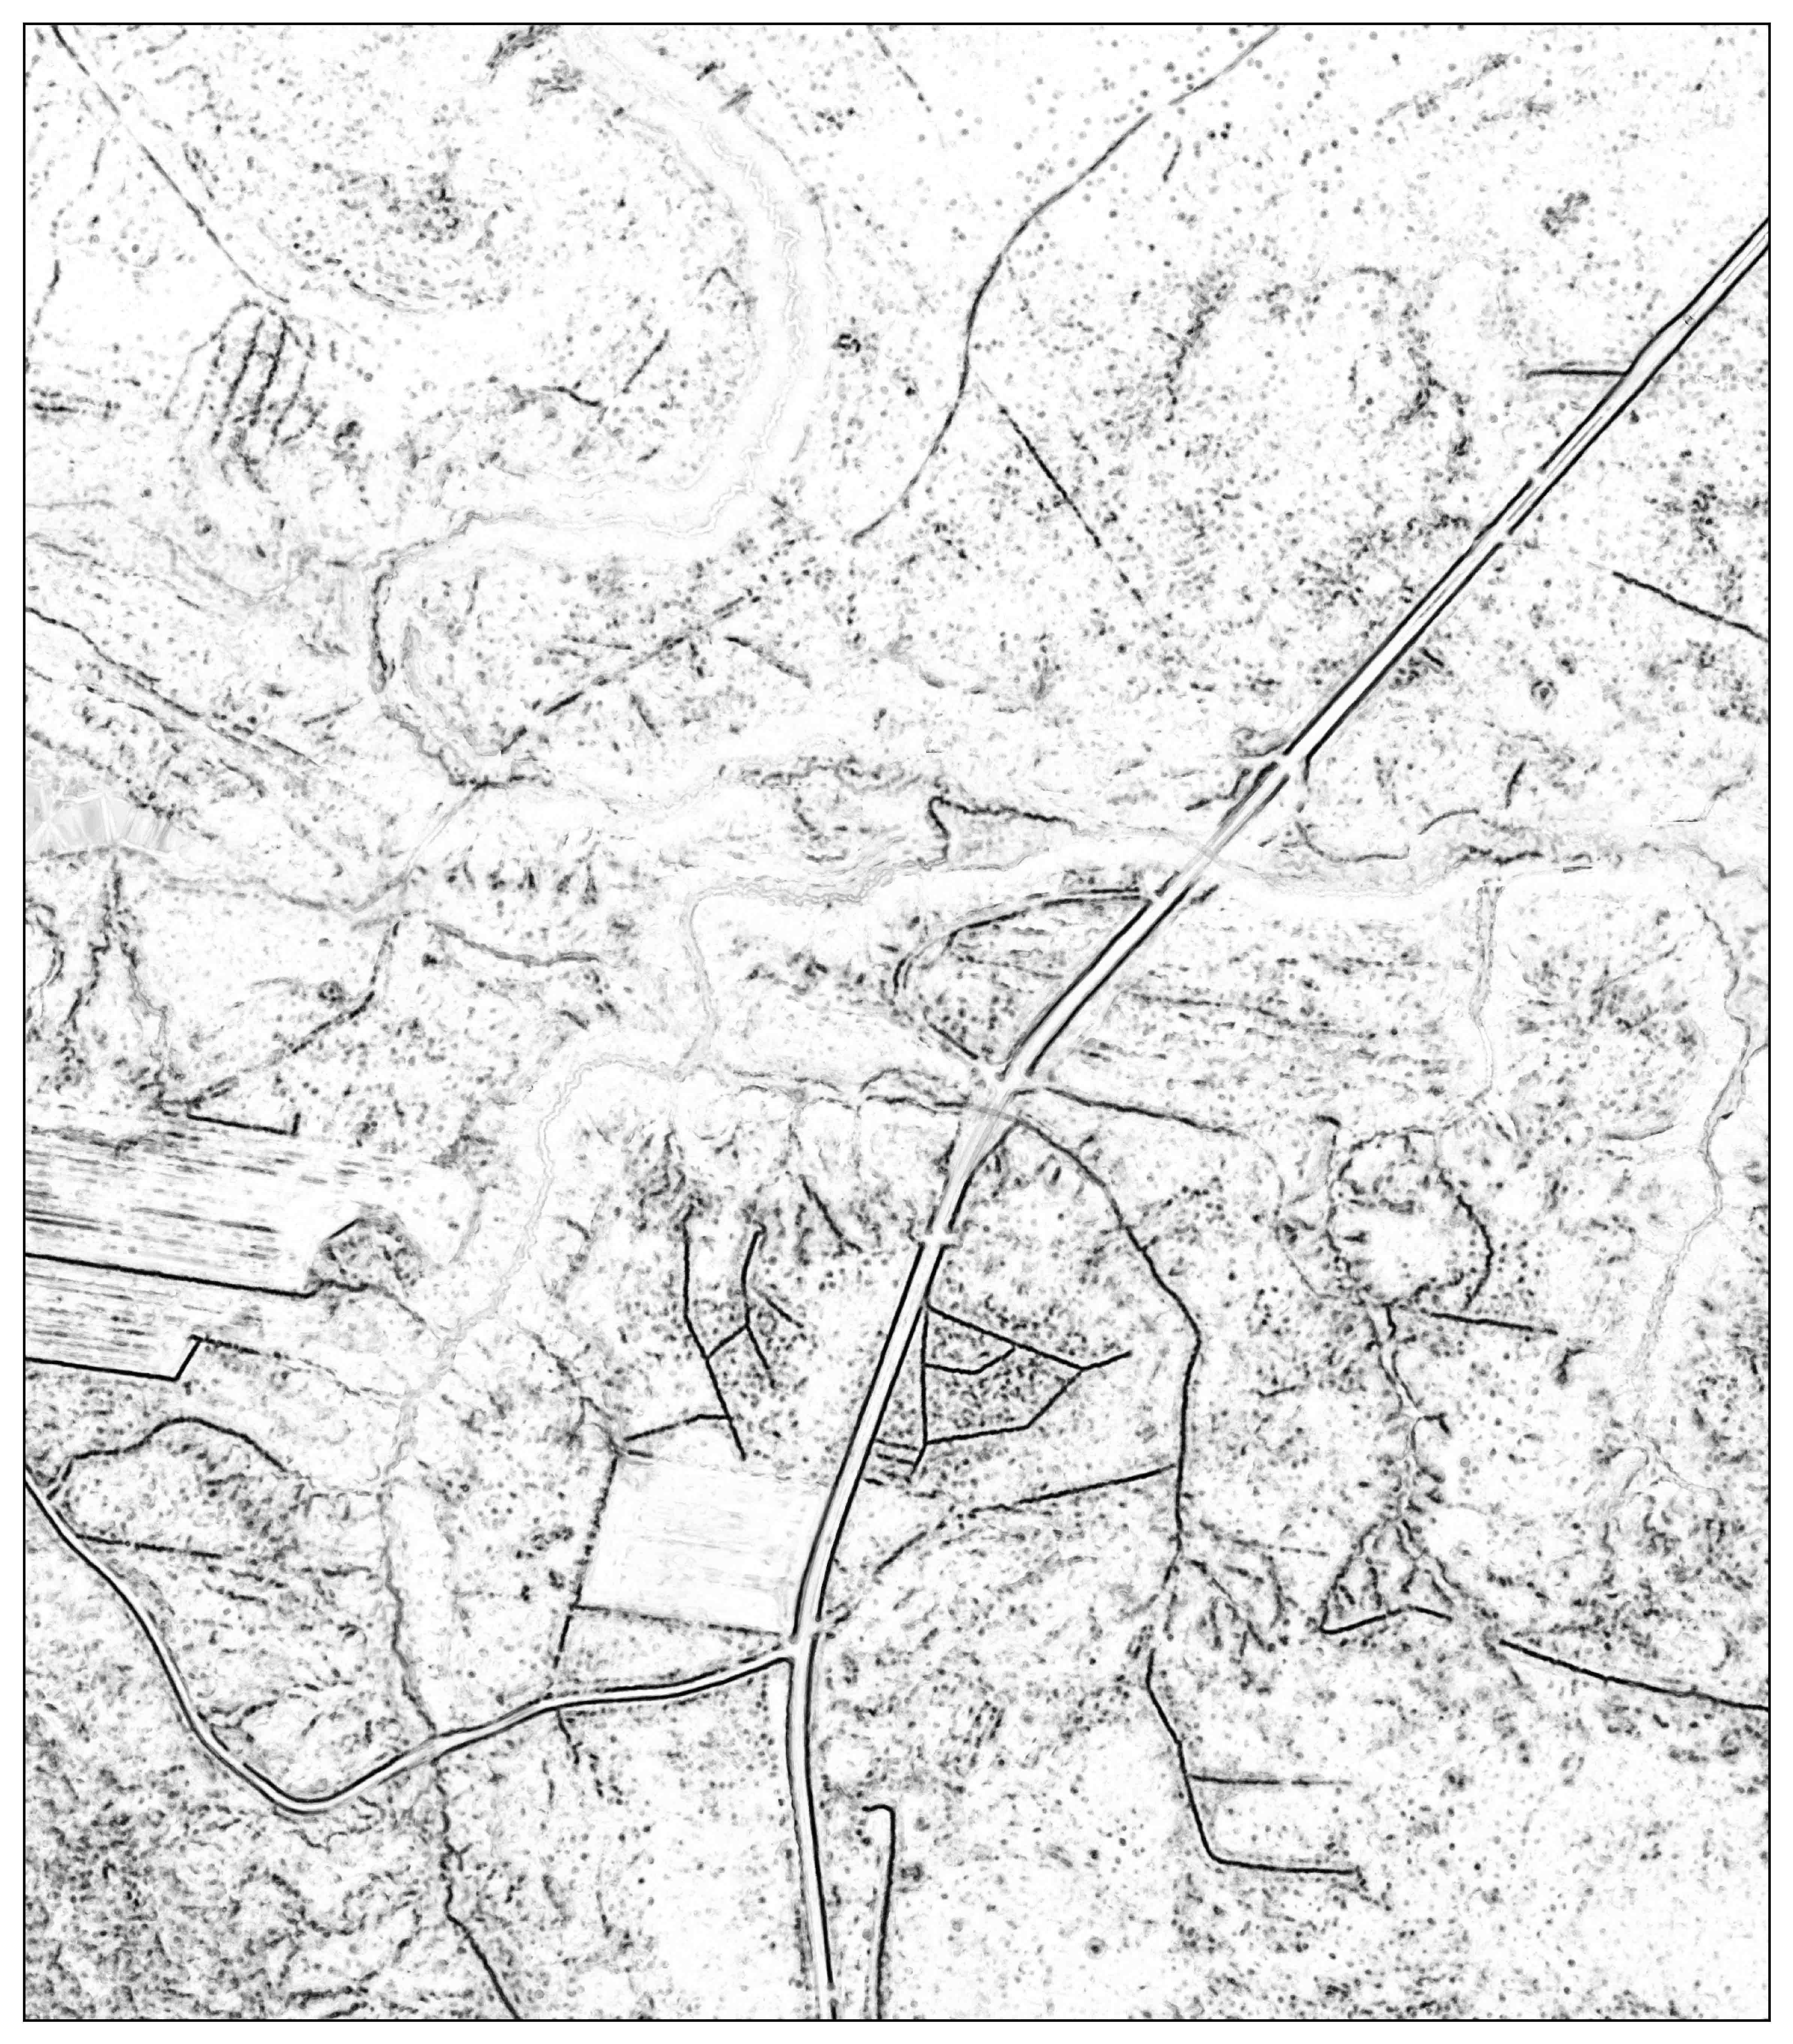
\includegraphics{./images/publ_post_process_step_1_lo.jpg}}}%%%
\DIFdelFL{\hspace{5pt}
    }%DIFDELCMD < \subfigure[]{
%DIFDELCMD <         \resizebox*{6.85cm}{!}{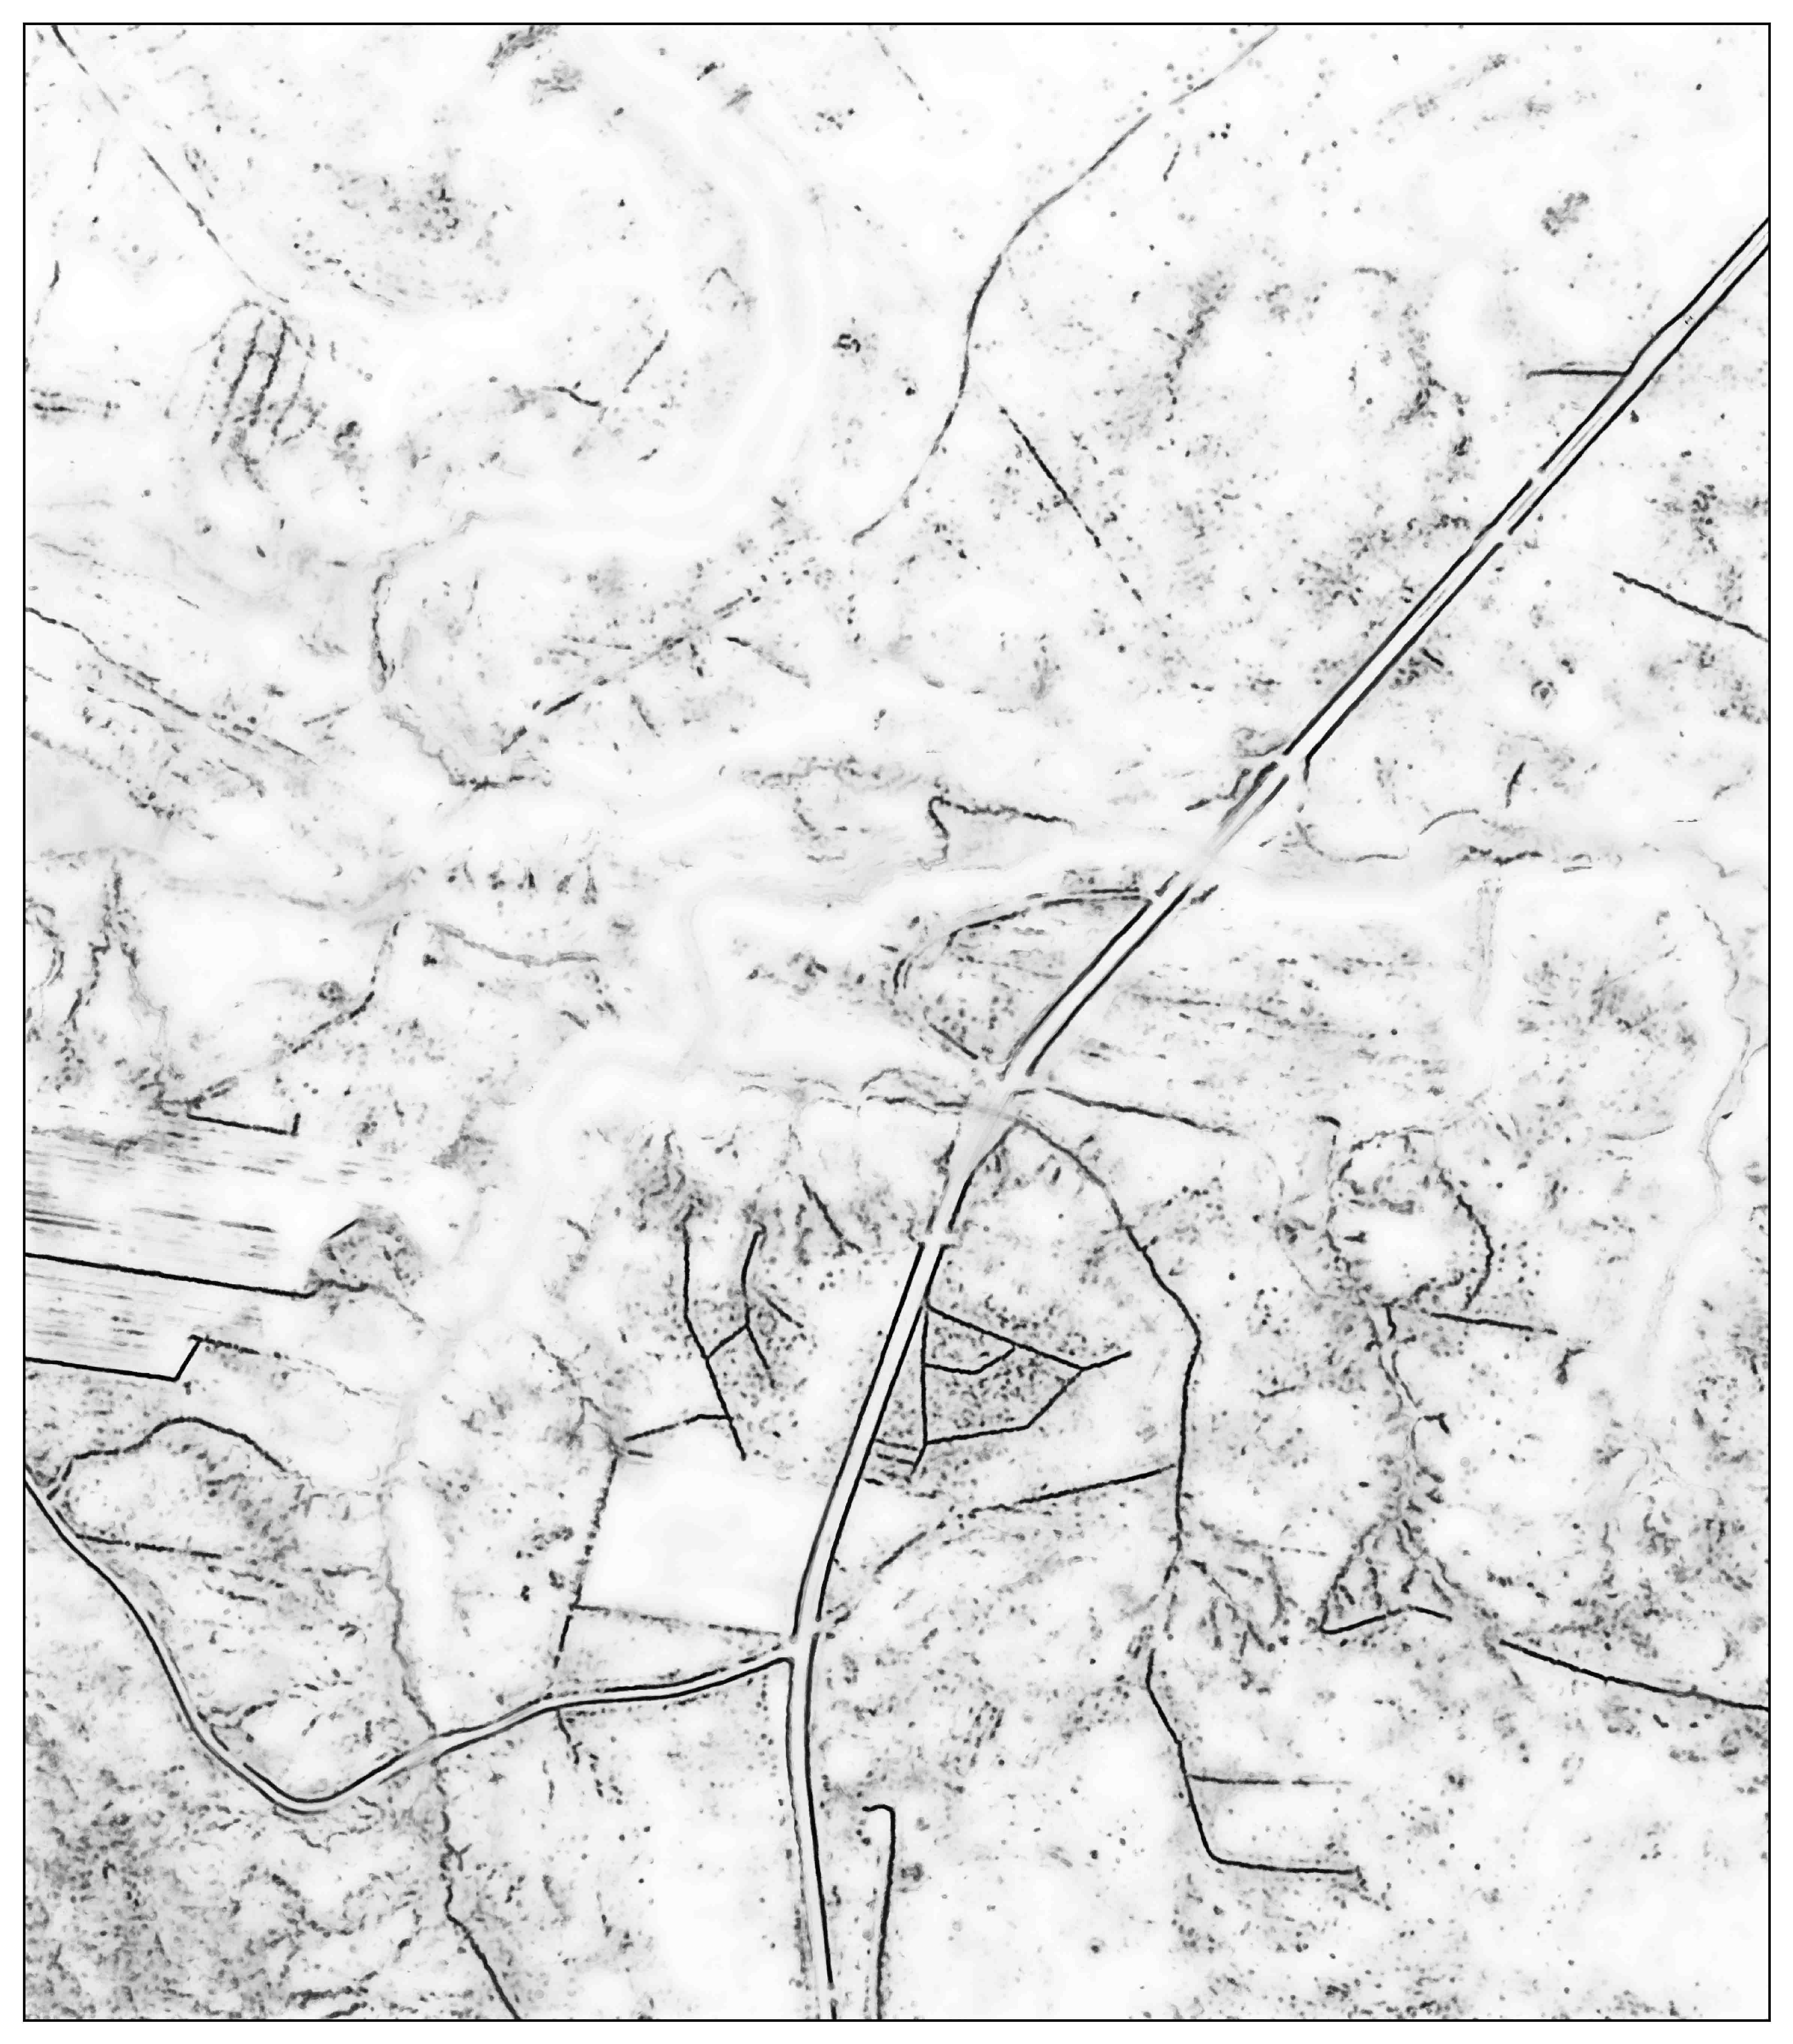
\includegraphics{./images/publ_post_process_step_2_lo.jpg}}}
%DIFDELCMD <     %%%
%DIFDELCMD < \caption{%
{%DIFAUXCMD
\DIFdelFL{Step one and two of the post-process. Darker pixels indicate a higher ditch probability. }\textbf{\DIFdelFL{a: }}%DIFAUXCMD
\DIFdelFL{Raw probability prediction produced by the Random Forests model. }\textbf{\DIFdelFL{b: }}%DIFAUXCMD
\DIFdelFL{Prediction after bilateral de-noising.}}
    %DIFAUXCMD
%DIFDELCMD < \label{fig:postprocessing1}
%DIFDELCMD < \end{figure}
%DIFDELCMD < 

%DIFDELCMD < %%%
\DIFdel{The second step for removing noise was to use a custom function to remove pixels that had a semi-high ditch probability, but that lay far away from any other high probability pixels. A threshold value was used to avoid removing pixels with a high enough ditch probability, helping to retain pixels that lay in or close to a ditch. The max ditch probability value in a circular radius of 10 pixels was then calculated. If this max value was too low, the probability value of the examined pixel was lowered }\DIFdelend (\hyperref[fig:postprocessing2]{Figure} \ref{fig:postprocessing2} \hyperref[fig:postprocessing2]{a}).

\DIFdelbegin \DIFdel{The third step involved taking measures to try to }\DIFdelend \DIFaddbegin \DIFadd{To }\DIFaddend fill gaps in ditches that the \DIFdelbegin \DIFdel{model }\DIFdelend \DIFaddbegin \DIFadd{models }\DIFaddend failed to correctly predict\DIFdelbegin \DIFdel{. A similar method to the one described in \ref{skyviewconic} was employed to calculate the mean of }\DIFdelend \DIFaddbegin \DIFadd{, we aggregated pixel values by covering them with }\DIFaddend cone masks expanding outwards in different directions from the examined pixel. This \DIFdelbegin \DIFdel{step also }\DIFdelend amplified some of the noise that was left, but filling the gaps in the ditches was judged to be more important \DIFdelbegin \DIFdel{to help make the next step more effective }\DIFdelend (\hyperref[fig:postprocessing2]{Figure} \ref{fig:postprocessing2} \hyperref[fig:postprocessing2]{b}).

\begin{figure} [!htb]
    \centering
    \DIFaddbeginFL \subfigure[]{
        \resizebox*{6.85cm}{!}{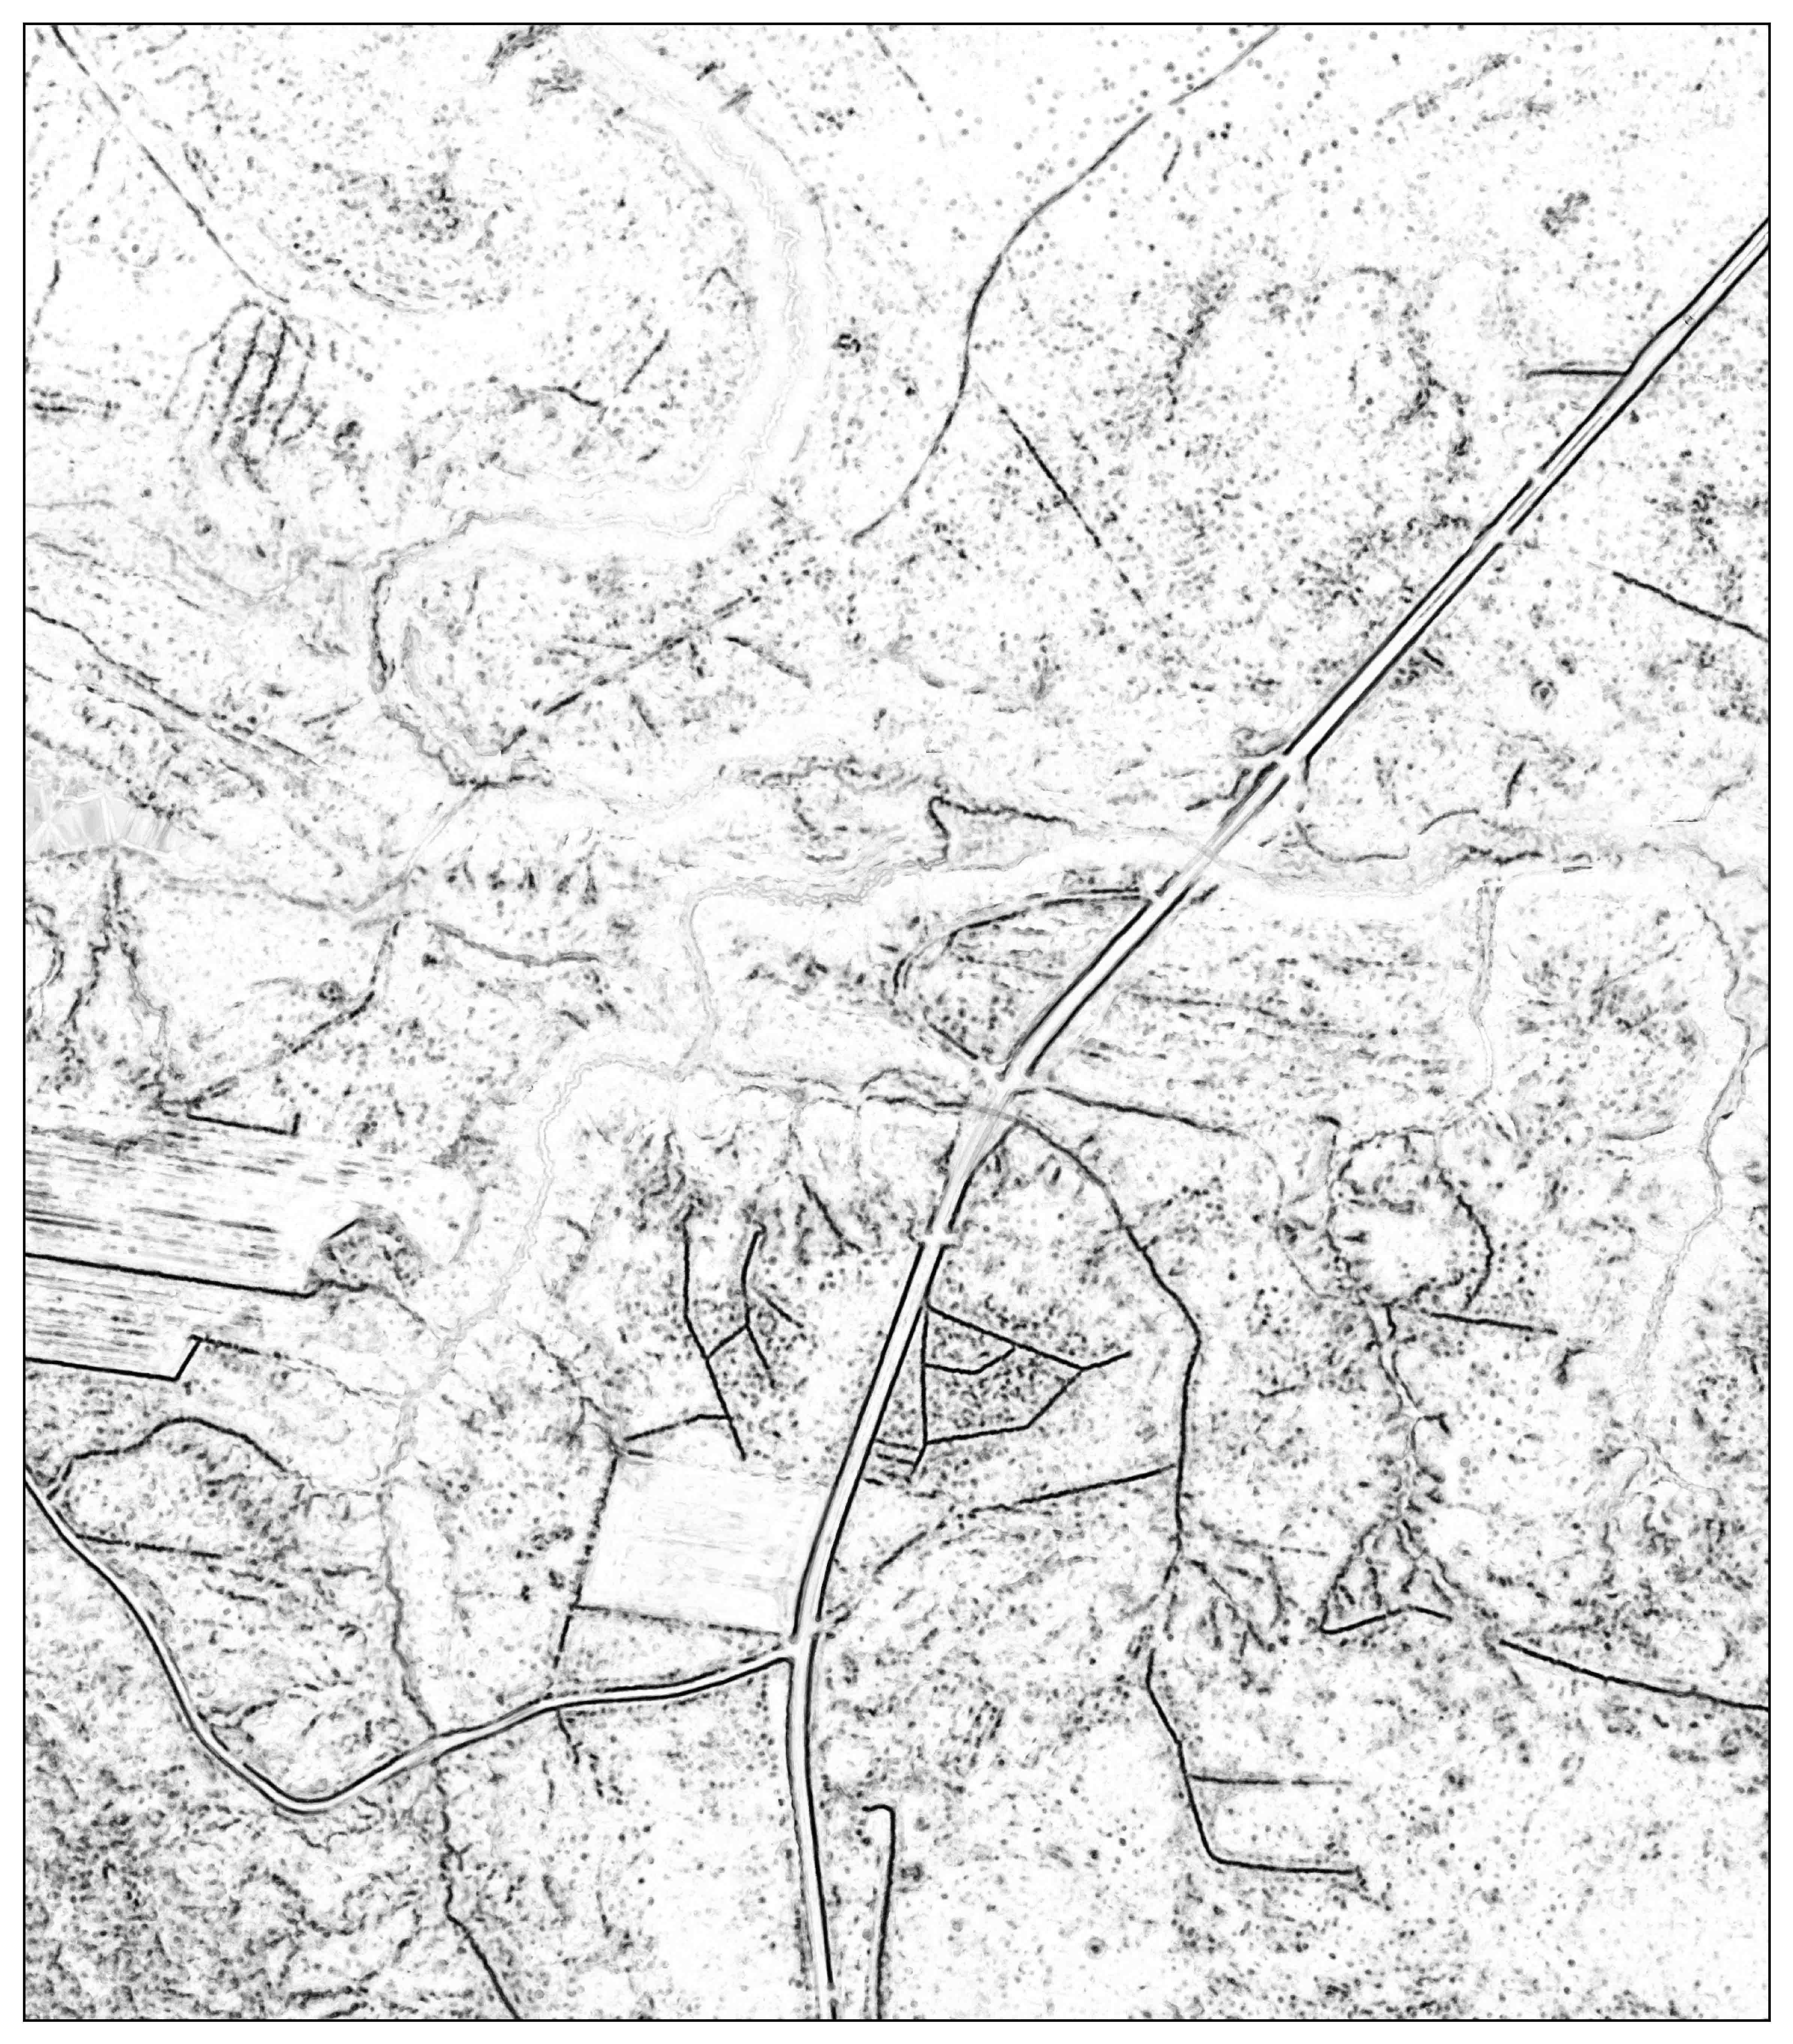
\includegraphics{./images/publ_post_process_step_1_lo.jpg}}}\DIFaddFL{\hspace{5pt}
    }\subfigure[]{
        \resizebox*{6.85cm}{!}{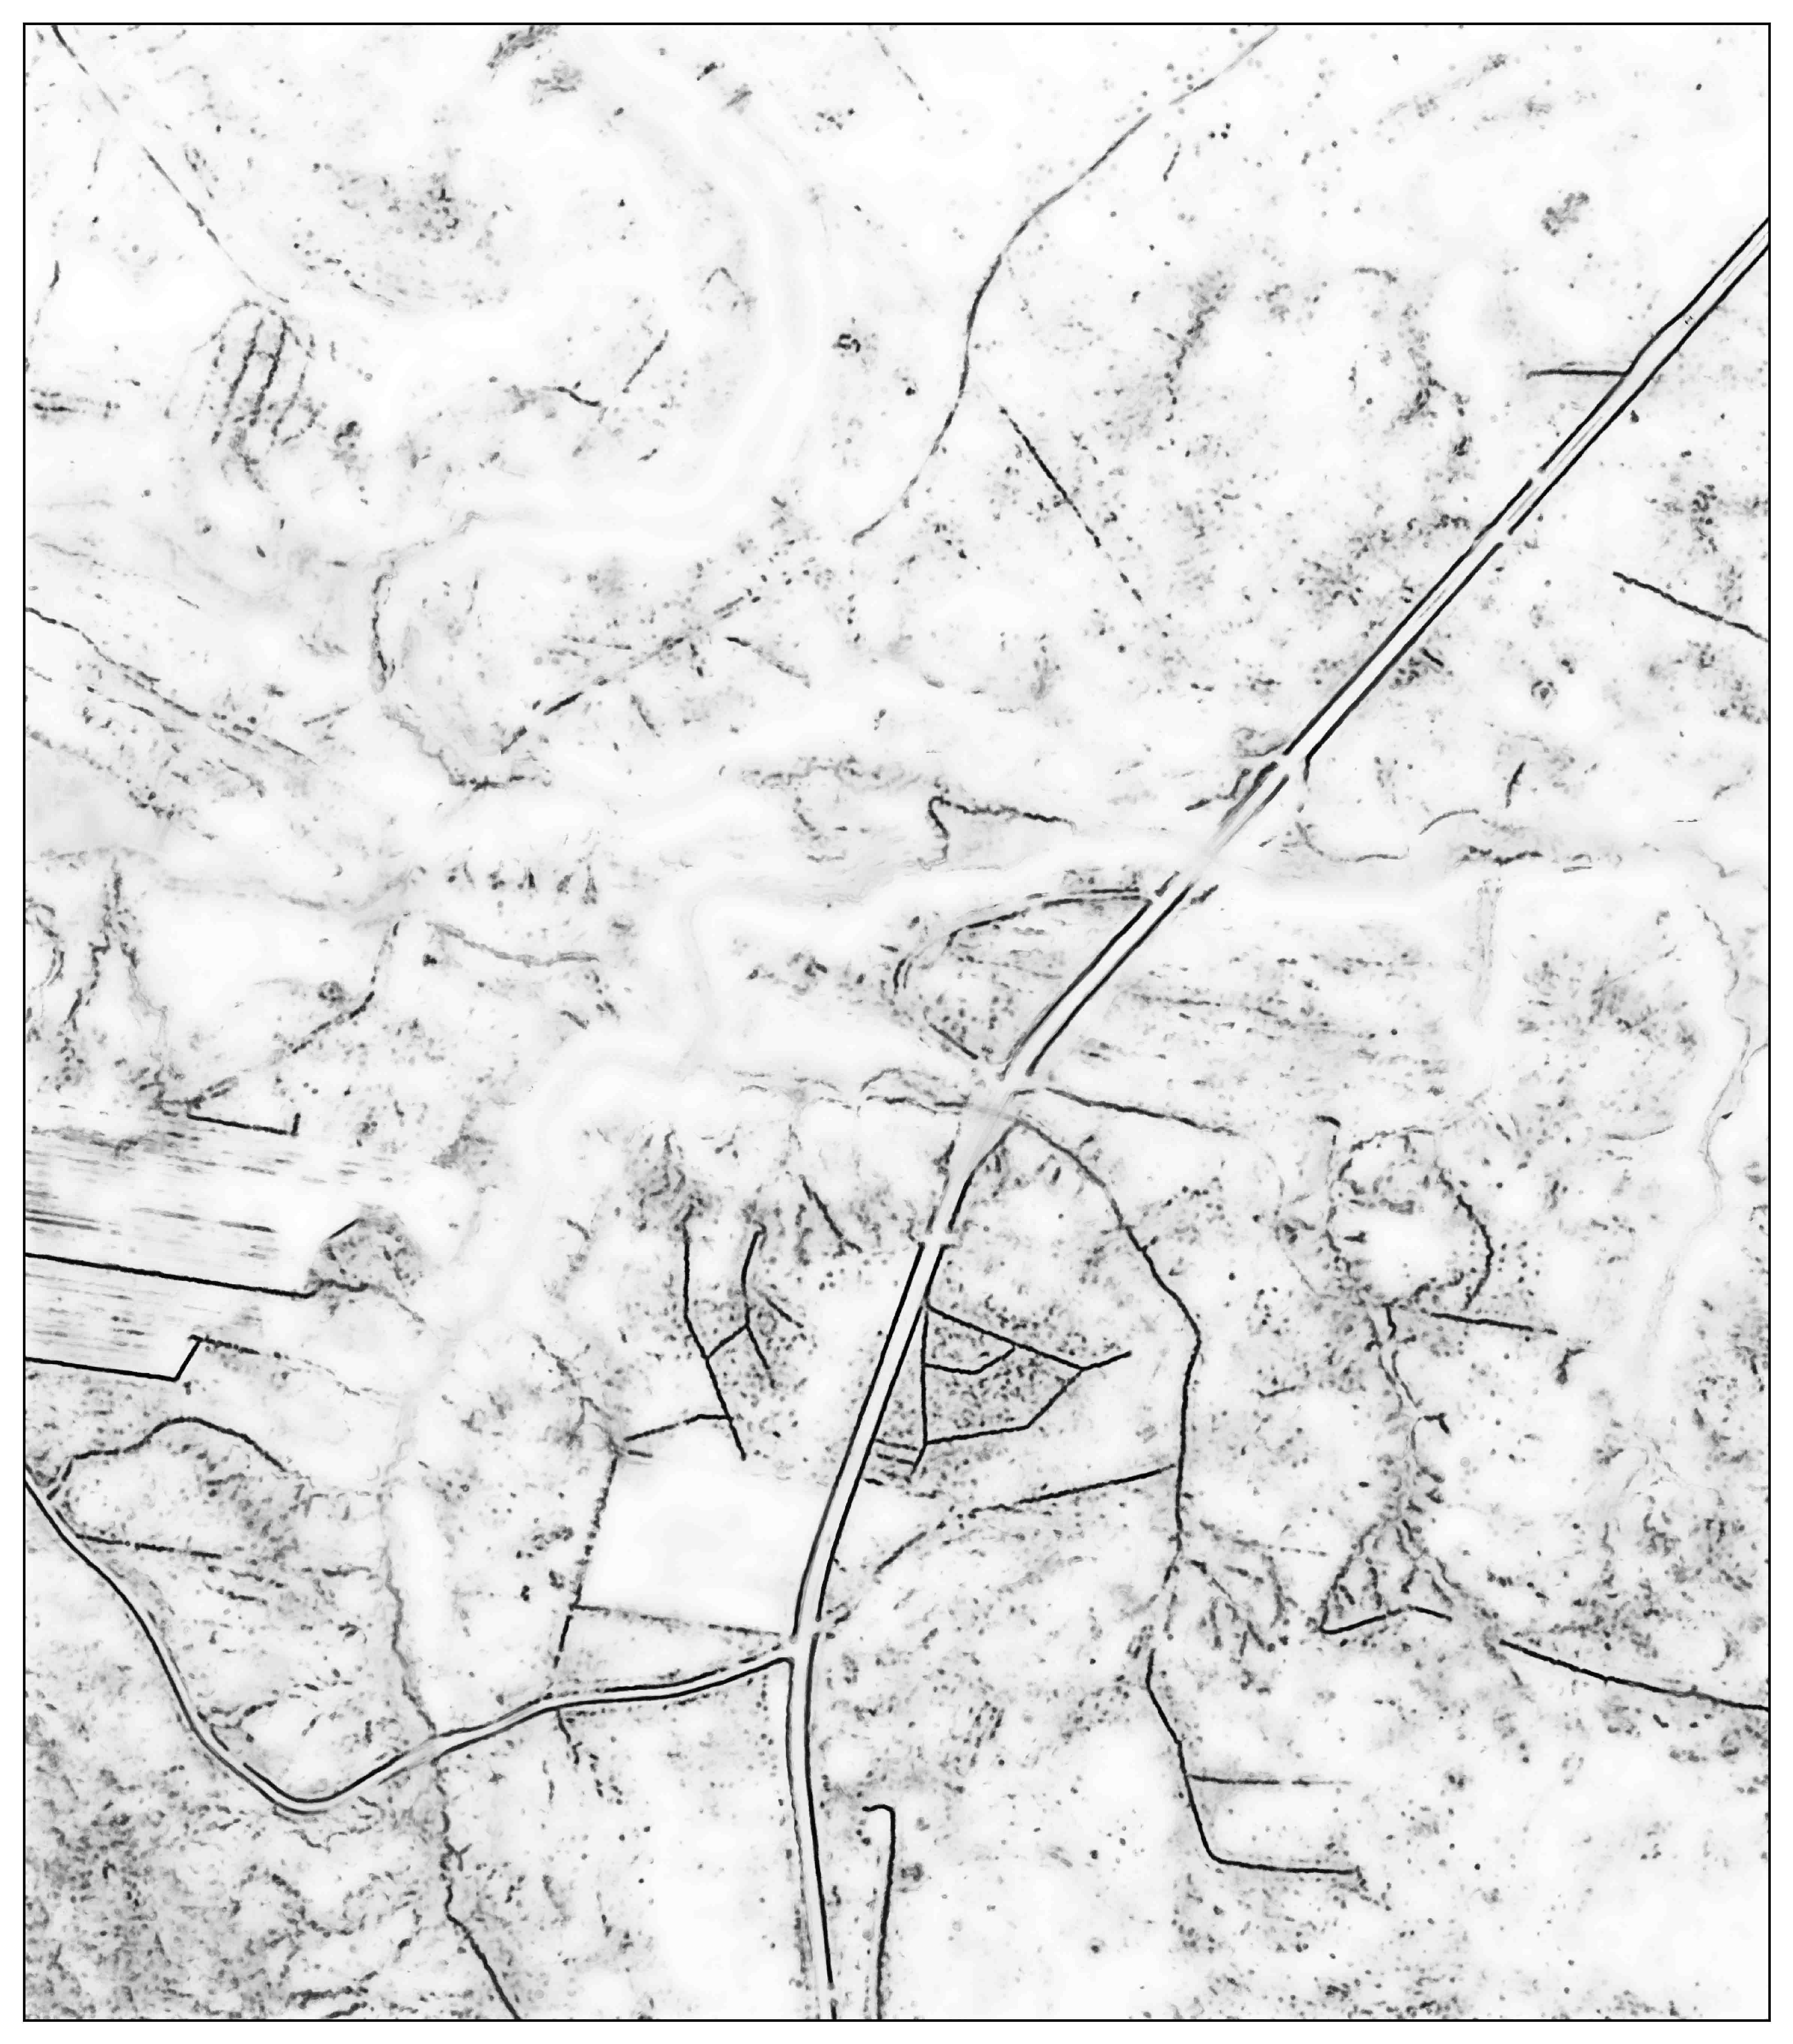
\includegraphics{./images/publ_post_process_step_2_lo.jpg}}}
    \caption{\DIFaddFL{Step one and two of the post-process. Darker pixels indicate a higher ditch probability. }\textbf{\DIFaddFL{a: }}\DIFaddFL{Random Forests probability prediction. }\textbf{\DIFaddFL{b: }}\DIFaddFL{Bilateral de-noising.}}
    \label{fig:postprocessing1}
\end{figure}

\begin{figure} [!htb]
    \centering
    \DIFaddendFL \subfigure[]{
        \resizebox*{6.85cm}{!}{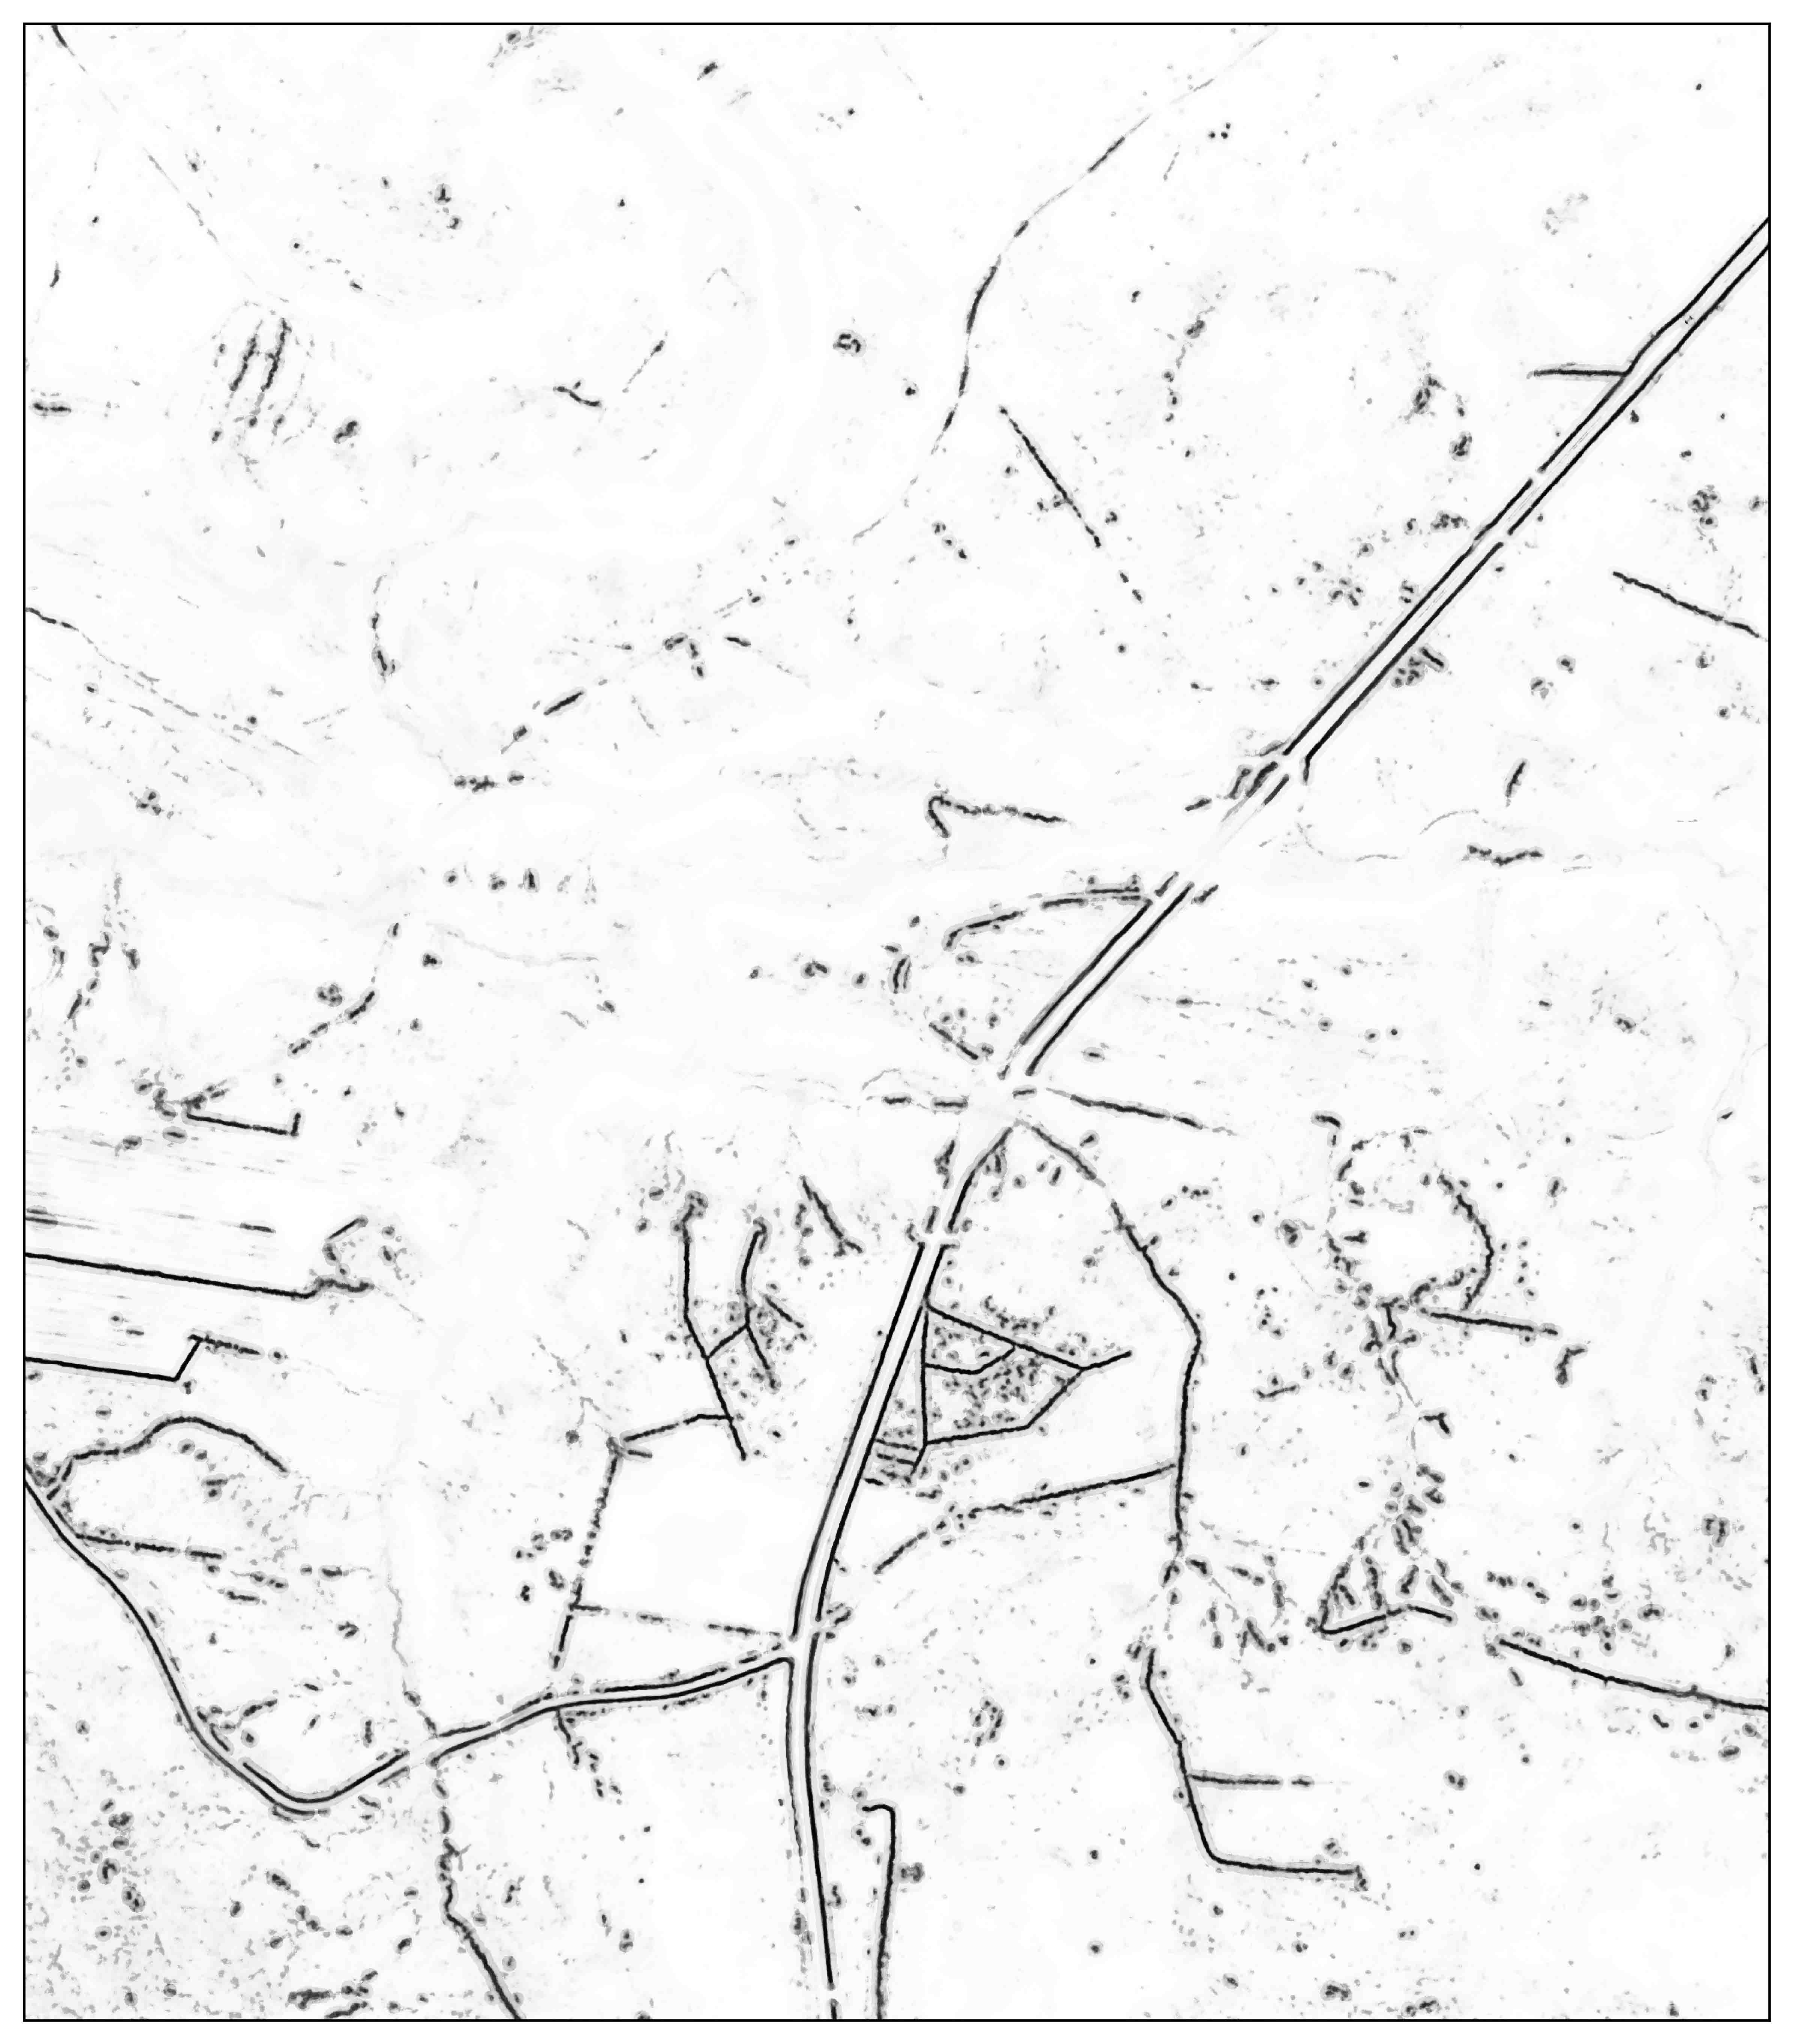
\includegraphics{./images/publ_post_process_step_3_lo.jpg}}}\hspace{5pt}
    \subfigure[]{
        \resizebox*{6.85cm}{!}{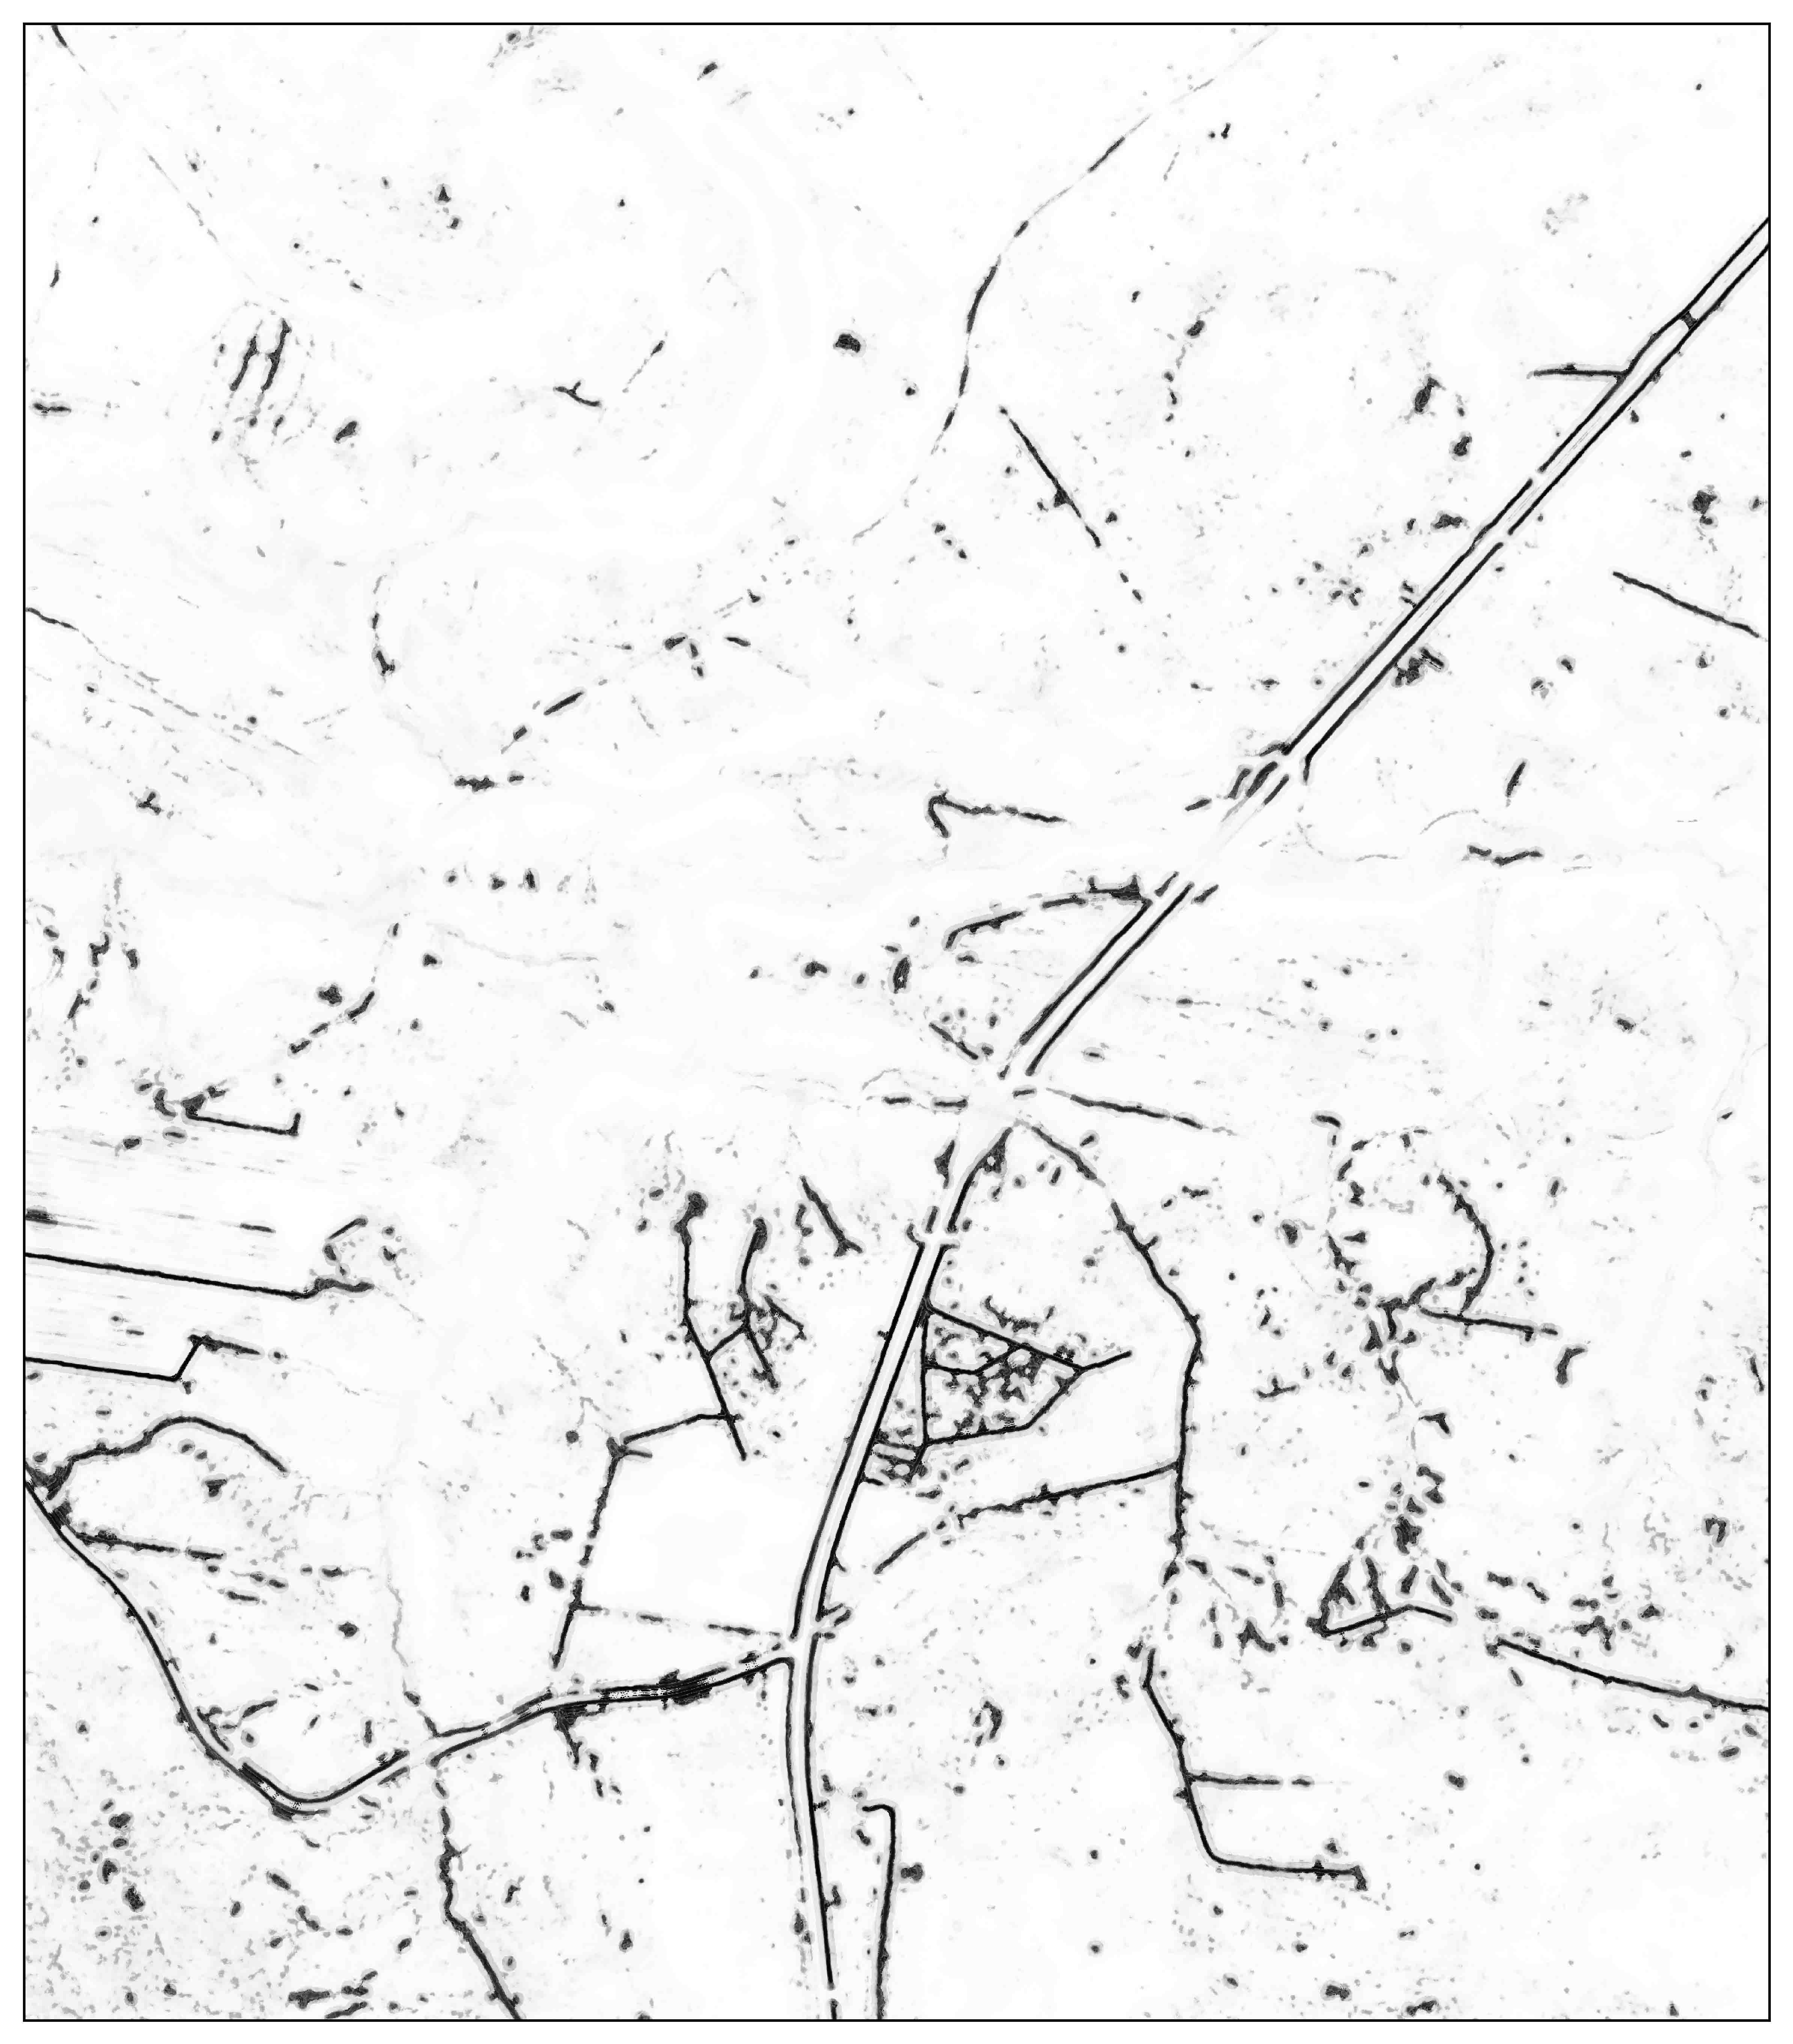
\includegraphics{./images/publ_post_process_step_4_lo.jpg}}}
    \caption{Step three and four of the post-process. Darker pixels indicate a higher ditch probability. \textbf{a: }\DIFdelbeginFL \DIFdelFL{Prediction after custom }\DIFdelendFL \DIFaddbeginFL \DIFaddFL{Custom }\DIFaddendFL de-noising. \textbf{b: }\DIFdelbeginFL \DIFdelFL{Prediction after gap }\DIFdelendFL \DIFaddbeginFL \DIFaddFL{Gap }\DIFaddendFL filling.}
    \label{fig:postprocessing2}
\end{figure}

\subsubsection{Binarisation with grid zones}
The \DIFdelbegin \DIFdel{model' s }\DIFdelend \DIFaddbegin \DIFadd{models' }\DIFaddend ditch prediction is given in the original resolution raster format. To allow for comparison to the evaluation data, the same grid conversion was performed on the prediction raster as on the evaluation data \DIFdelbegin \DIFdel{seen }\DIFdelend \DIFaddbegin \DIFadd{displayed }\DIFaddend in \hyperref[fig:ditchpreprocess]{Figure} \ref{fig:ditchpreprocess} \hyperref[fig:ditchpreprocess]{c}. \DIFdelbegin \DIFdel{A }\DIFdelend \DIFaddbegin \DIFadd{After testing different combinations of zone sizes and probability values, a }\DIFaddend mean probability rating was calculated for each $6*6$ grid zone, classifying the entire zone as part of a ditch if the mean probability exceeded \DIFdelbegin \DIFdel{35 }\DIFdelend \DIFaddbegin \DIFadd{40 }\DIFaddend \%. This \DIFaddbegin \DIFadd{zone partitioning }\DIFaddend helped to fill in gaps where lone pixels in ditches had been incorrectly classified\DIFdelbegin \DIFdel{, and also helped in the next step of the post-processing }\DIFdelend \DIFaddbegin \DIFadd{. }\DIFaddend (\hyperref[fig:postprocessing3]{Figure} \ref{fig:postprocessing3} \hyperref[fig:postprocessing3]{a}).

\subsubsection{Cluster removal}
To remove noise from the binary prediction, a custom cluster detection algorithm was used. By finding the number of connected pixels with a true value and removing those whose cluster size were below a given threshold, minor noise in the prediction could be removed while still retaining most of the ditch pixels. Actual ditches that have a low probability and therefore create small clusters may still be excluded by this method, but the noise removal advantages were judged to outweigh the loss in recall. A distance calculation was also performed in tandem with this method to find the largest distance of pixels inside each given cluster. This helped to remove \DIFdelbegin \DIFdel{cavities }\DIFdelend \DIFaddbegin \DIFadd{sinks }\DIFaddend and hollows that were not removed by the initial small cluster removal, but that \DIFdelbegin \DIFdel{had a shape that indicated that }\DIFdelend \DIFaddbegin \DIFadd{did not have a linear directional characteristic, indicating that }\DIFaddend they did not represent a ditch (\hyperref[fig:postprocessing3]{Figure} \ref{fig:postprocessing3} \hyperref[fig:postprocessing3]{b}).

\begin{figure} [!htb]
    \centering
    \subfigure[]{
        \resizebox*{6.85cm}{!}{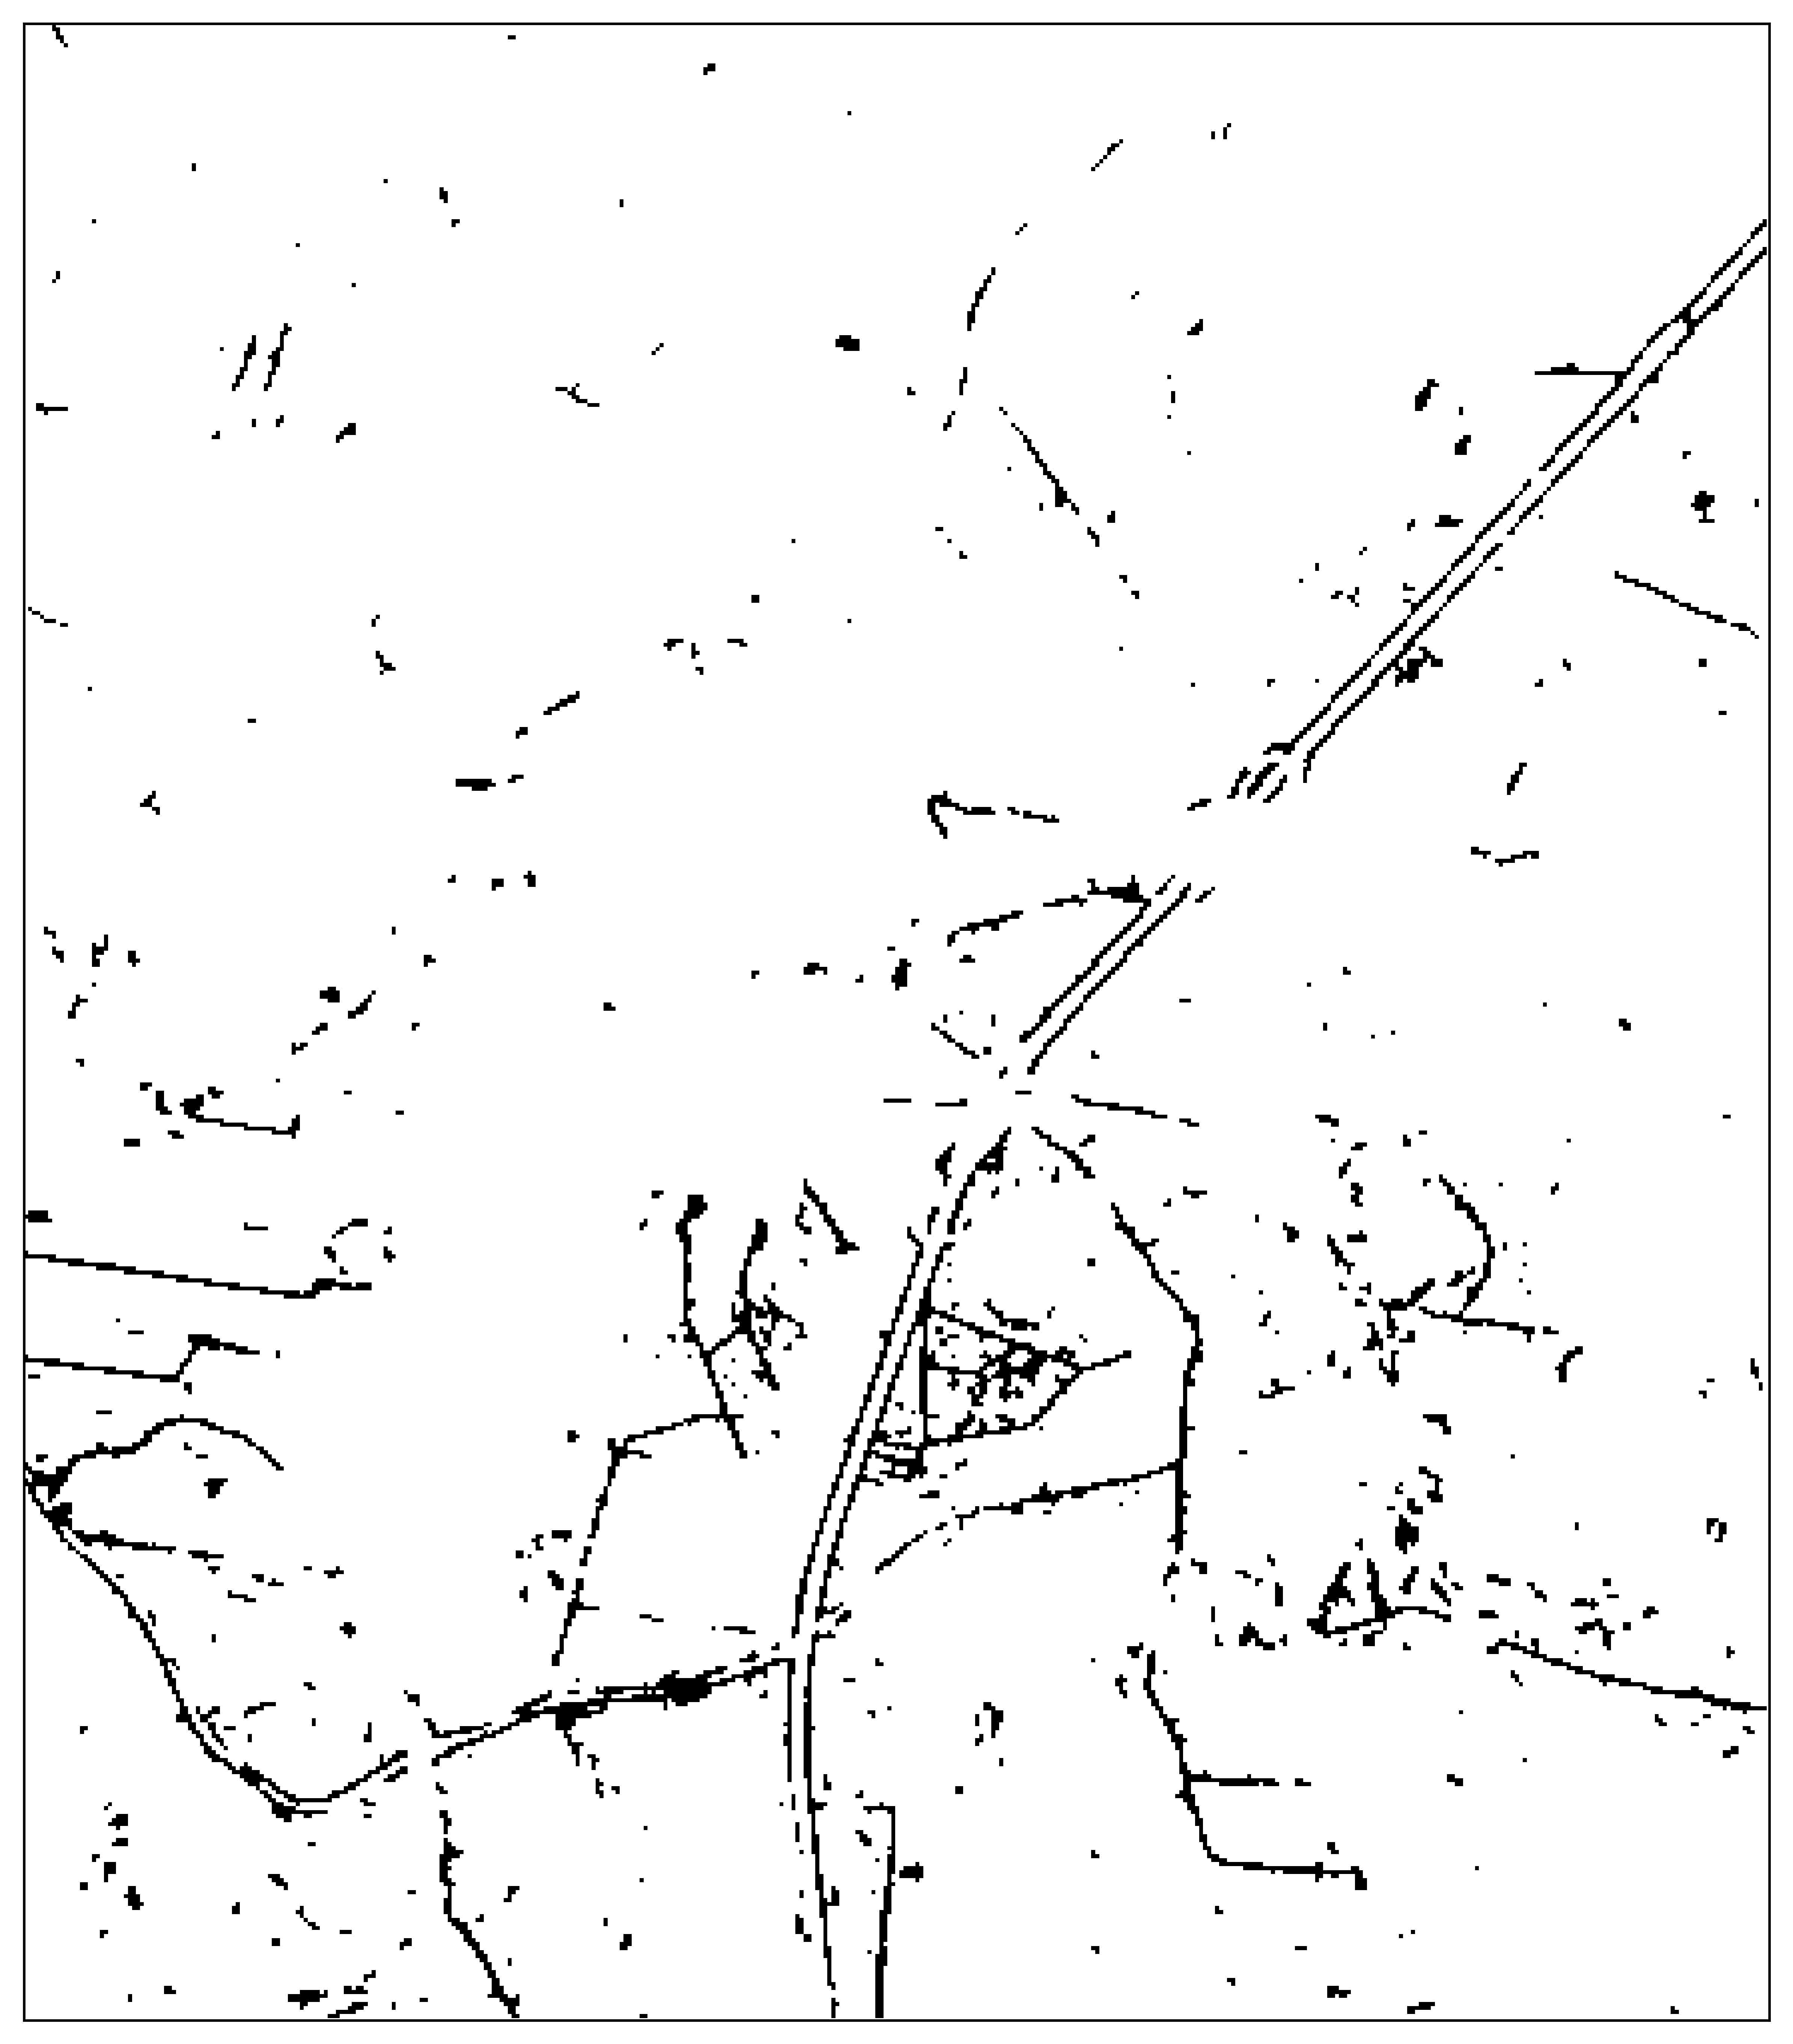
\includegraphics{./images/publ_post_process_step_5_lo.jpg}}}\hspace{5pt}
    \subfigure[]{
        \resizebox*{6.85cm}{!}{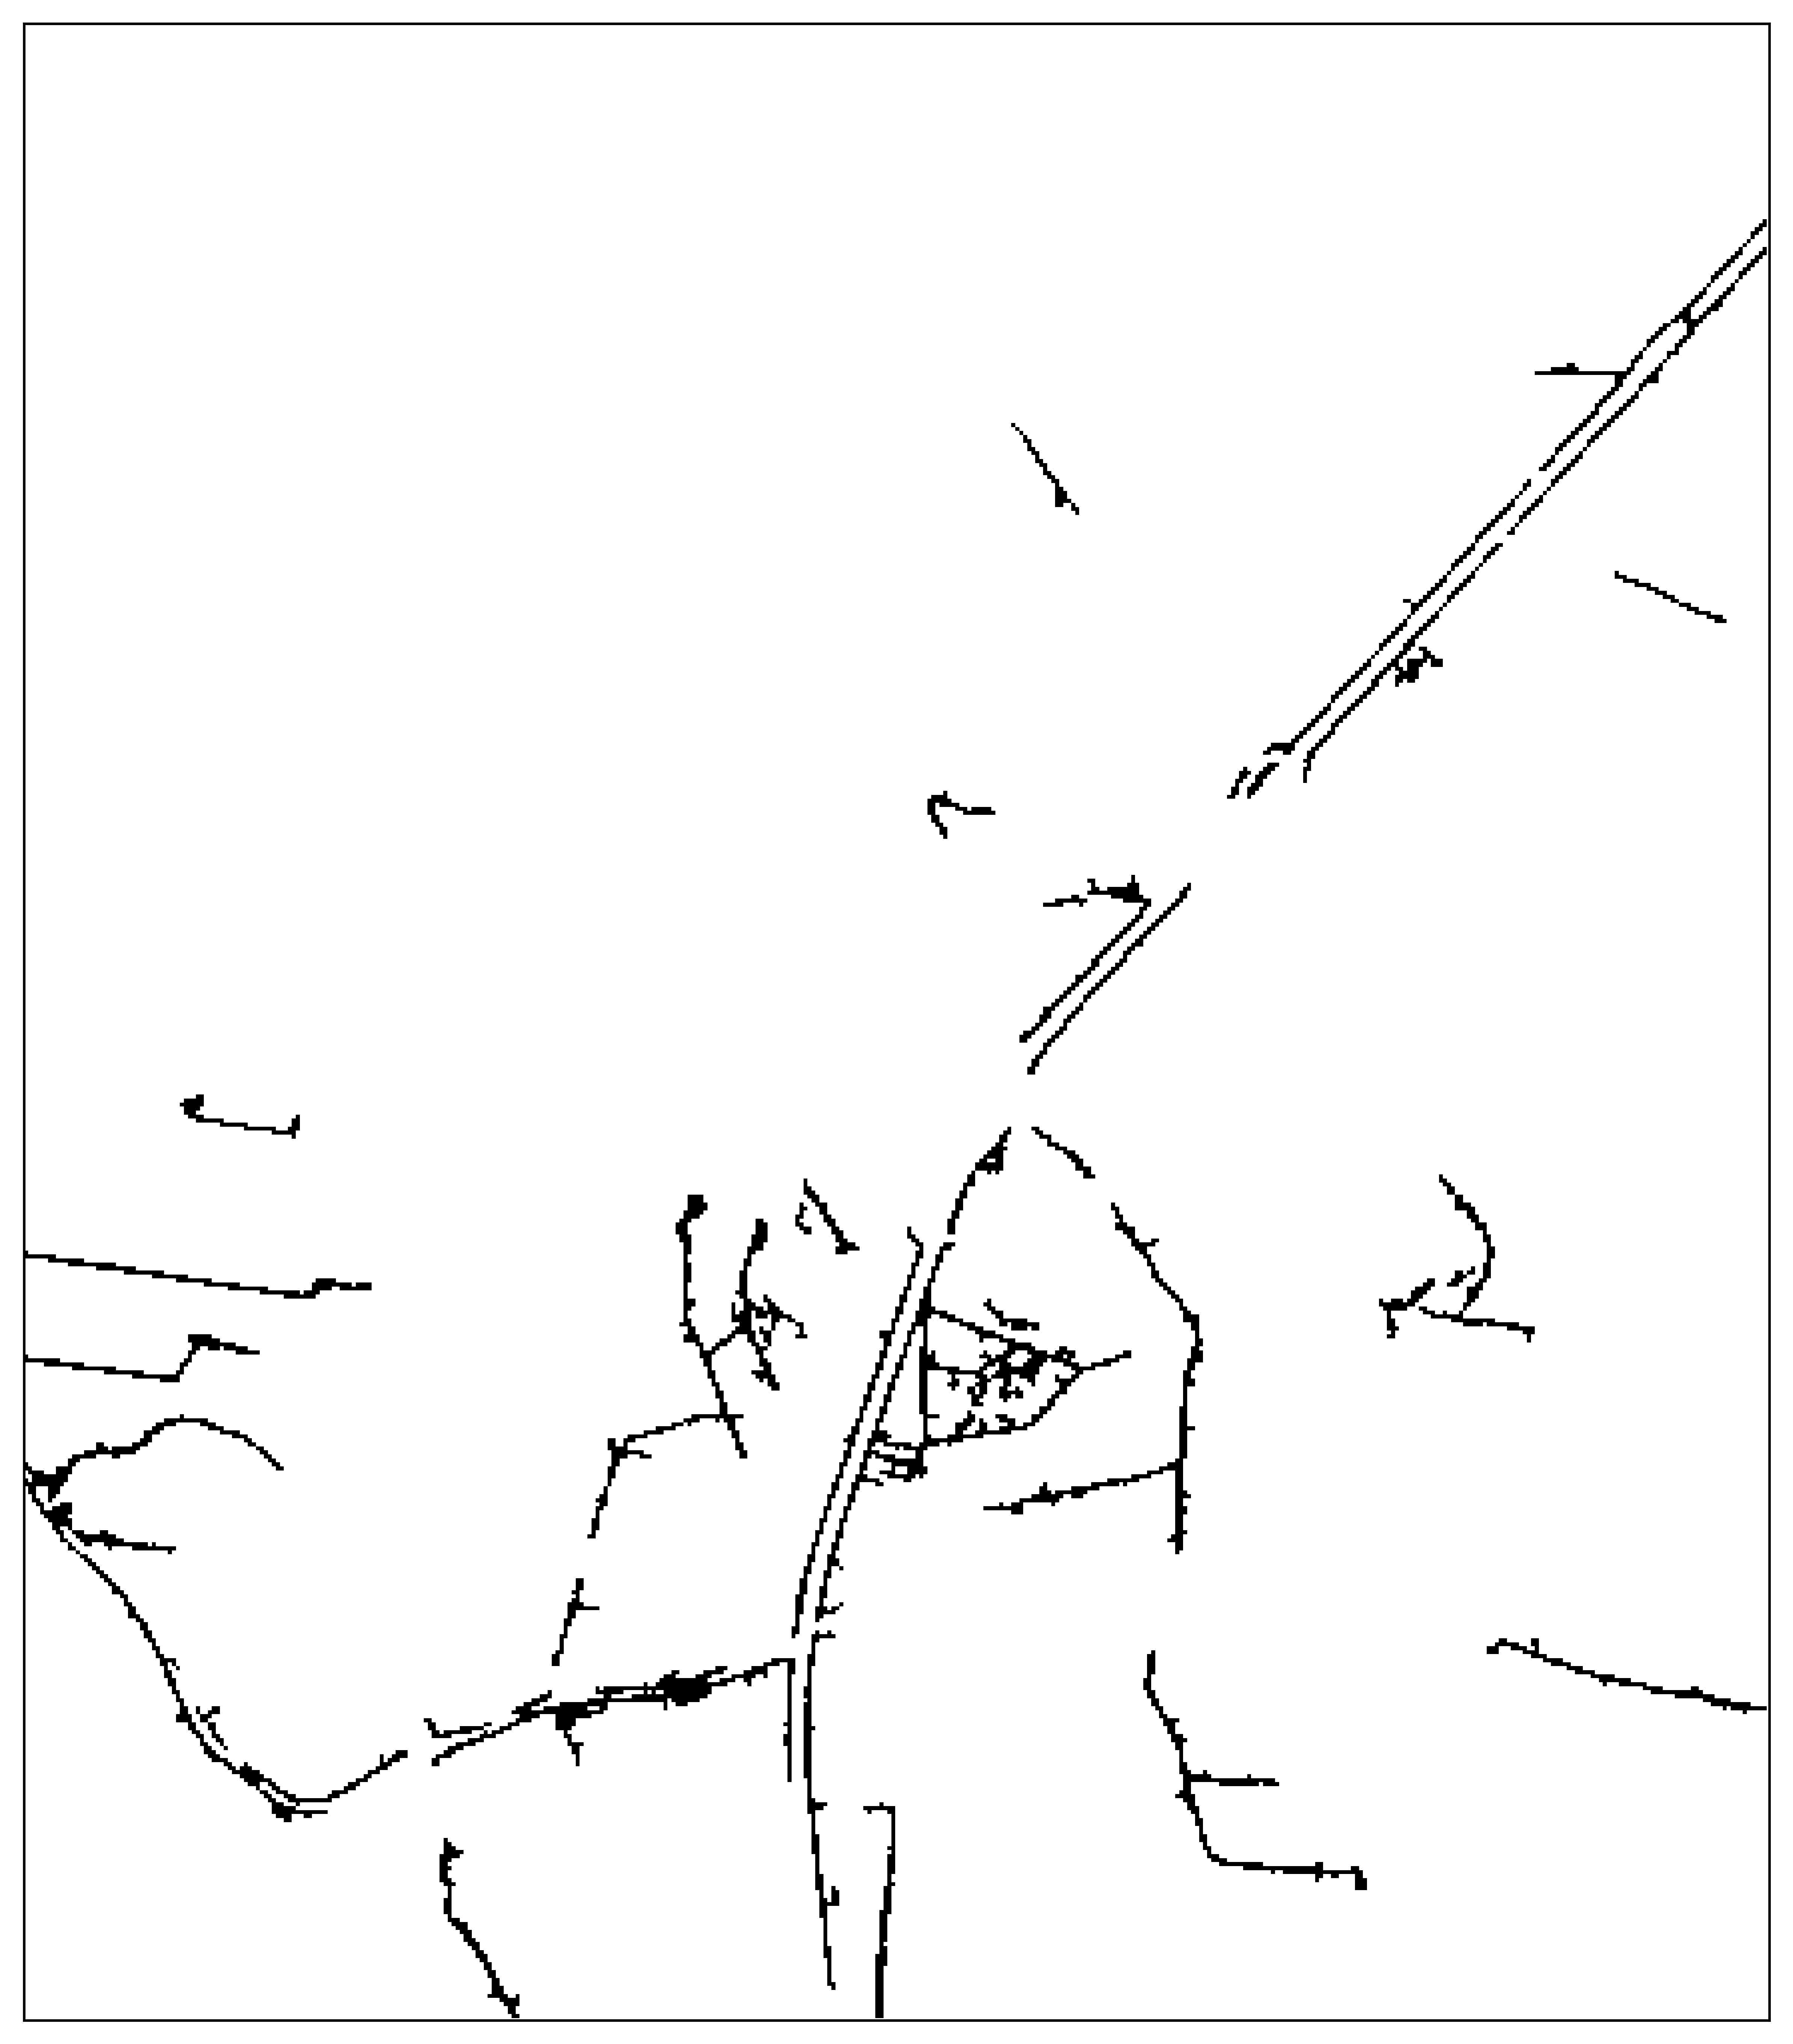
\includegraphics{./images/publ_post_process_step_6_lo.jpg}}}
    \caption{Step five and six of the post-process. Black pixels indicate a ditch prediction. \textbf{a: }\DIFdelbeginFL \DIFdelFL{Prediction after binarisation with grid }\DIFdelendFL \DIFaddbeginFL \DIFaddFL{Grid }\DIFaddendFL zone \DIFdelbeginFL \DIFdelFL{probability. }\DIFdelendFL \DIFaddbeginFL \DIFaddFL{binarisation }\DIFaddendFL \textbf{b: }\DIFdelbeginFL \DIFdelFL{Final binary prediction after cluster }\DIFdelendFL \DIFaddbeginFL \DIFaddFL{Cluster }\DIFaddendFL removal.}
    \label{fig:postprocessing3}
\end{figure}

\subsection{Evaluation} \label{evaluation}

Using only accuracy as an evaluation metric when dealing with an imbalanced dataset (roughly 98 \% of all pixels are non-ditch) would produce a poor performance assessment \citep{balanced}; by simply classifying all pixels as non-ditches, we would by default attain 98 \% accuracy. For this reason, the results were mainly evaluated using Cohen's Kappa (Cohen's $\kappa$) index, and the Area under Precision-Recall curve. Cohen's $\kappa$ index measures how much better a prediction is compared to a \DIFdelbegin \DIFdel{prediction based purely on chance, where chance }\DIFdelend \DIFaddbegin \DIFadd{completely random prediction, where random }\DIFaddend would yield a value of zero \citep{kappa123}. With our data, a $\kappa$ value close to zero would be attained by predicting 2 \% of the occurrences as ditch pixels completely at random. Values above zero are better than \DIFdelbegin \DIFdel{chance }\DIFdelend \DIFaddbegin \DIFadd{random, }\DIFaddend and values below zero are worse than \DIFdelbegin \DIFdel{chance}\DIFdelend \DIFaddbegin \DIFadd{random}\DIFaddend .

\DIFdelbegin %DIFDELCMD < \newpage
%DIFDELCMD < 

%DIFDELCMD < %%%
\DIFdel{The chance }\DIFdelend \DIFaddbegin \DIFadd{The random }\DIFaddend rating $P_c$ of a prediction of $n$ occurrences is calculated with:\footnote{ P = Positive (ditch pixel), N = Negative (non-ditch pixel), T = true, F = false}

$$
P_c = \frac{\left(\frac{(TP + FN) \cdot (TP + FP)}{n}\right) + \left(\frac{(FN + TN) \cdot (FP + TN)}{n}\right)}{n}
$$

$$
\text{Cohen's } \kappa \text{ is then calculated as a value between -1 and 1 with:}
$$
$$\kappa = \frac{Accuracy - P_c}{1 - P_c}$$

The Precision-Recall curve and the Area under Precision-Recall curve (AUPRC) are additional metrics that can be used when evaluating datasets with a largely imbalanced class distribution \citep{precision_recall_curve}. The Precision-Recall curve has the recall value on the x-axis and the precision value on the y-axis, and the area under the curve that is defined by this point gives the AUPRC value. The area under this curve is given as a value between zero and one, where a value closer to one is better. The weighting causes the Precision-Recall curve to not place an equal value on true negatives and true positives \citep{precision_recall_curve}. For our ditch detection problem, this means that the AUPRC evaluation metric favours accurately classifying ditch pixels over accurately classifying non-ditch pixels.

To circumvent some of the performance evaluation issues arising from the use of pixel classification for ditch objects as well as not having completely accurate labels on a pixel basis (due to uncertainties in the width of the ditches), we modified the evaluation labels to allow for some error in close proximity to ditches in the prediction. False \DIFdelbegin \DIFdel{negatives }\DIFdelend \DIFaddbegin \DIFadd{negative }\DIFaddend and false positive grid zones that lay adjacent to the ditch label grid zones were evaluated as true negatives and true positives, as they can be considered a part of correctly located ditch objects (\hyperref[fig:newlabels]{Figure} \ref{fig:newlabels}).

\begin{figure} [!htb]
    \centering
    \subfigure[]{
        \resizebox*{6.5cm}{!}{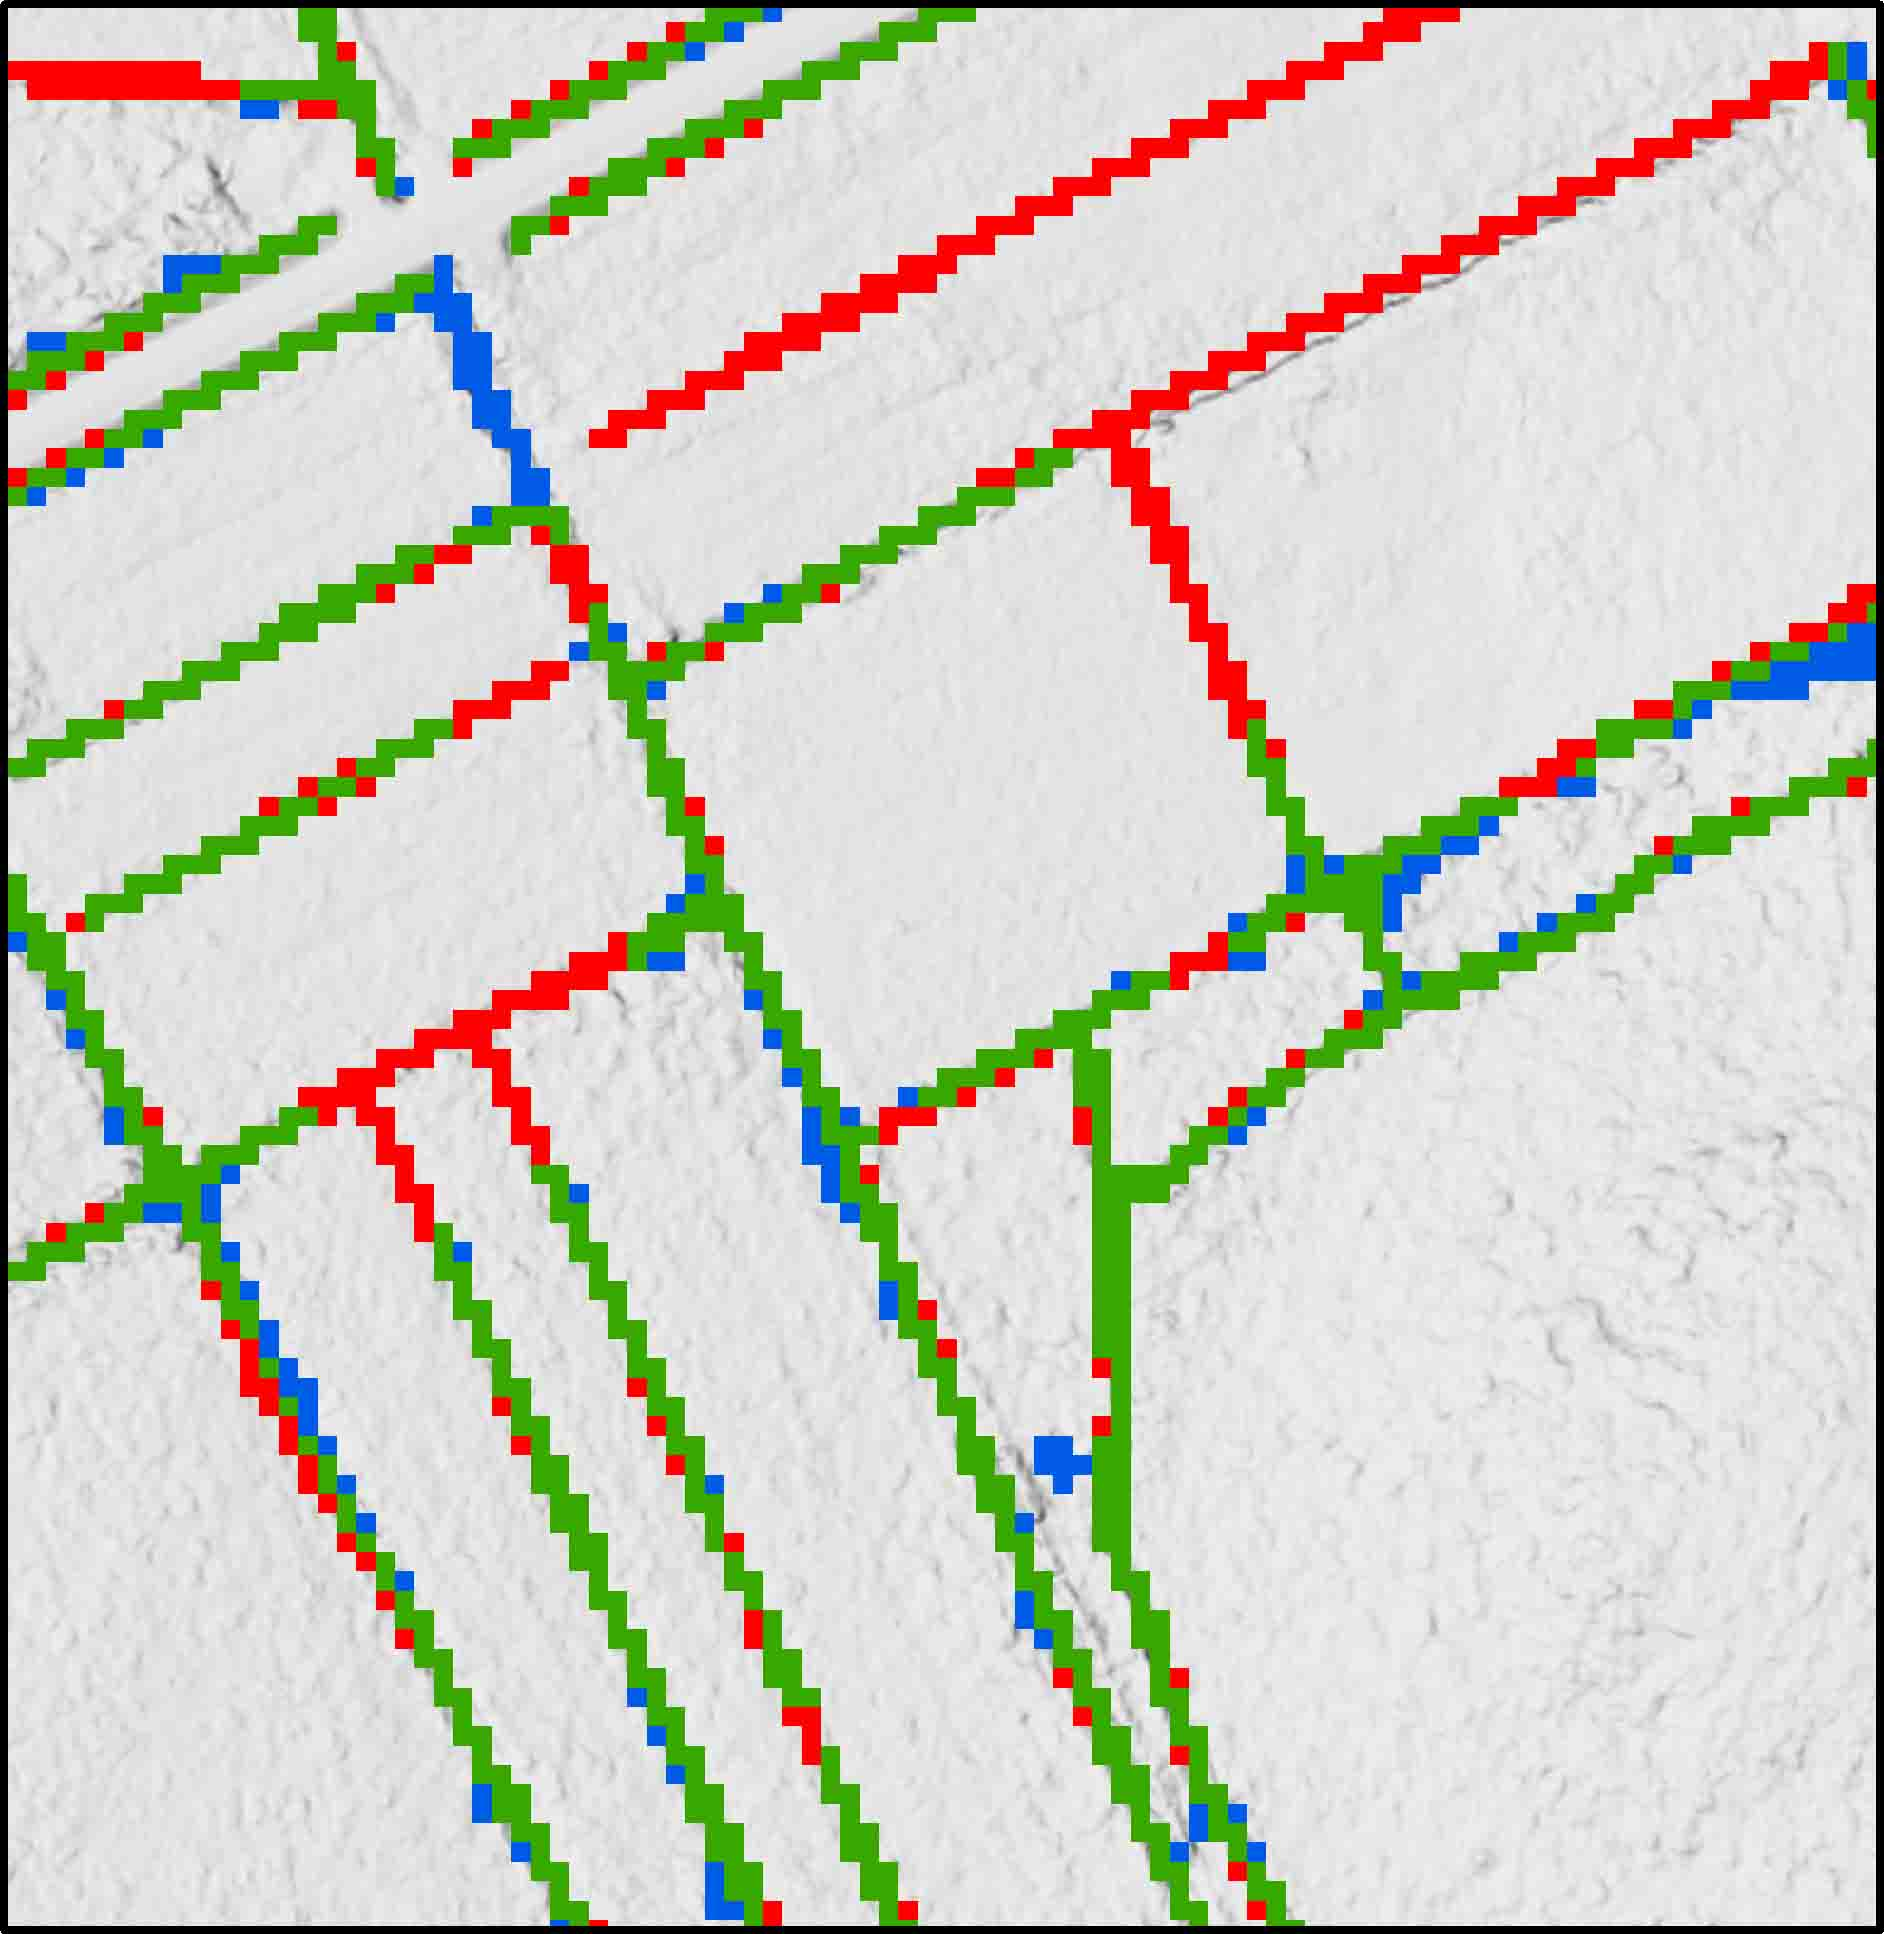
\includegraphics{./images/re_evaluation_1_lo.jpg}}}\hspace{5pt}
    \subfigure[]{
        \resizebox*{6.5cm}{!}{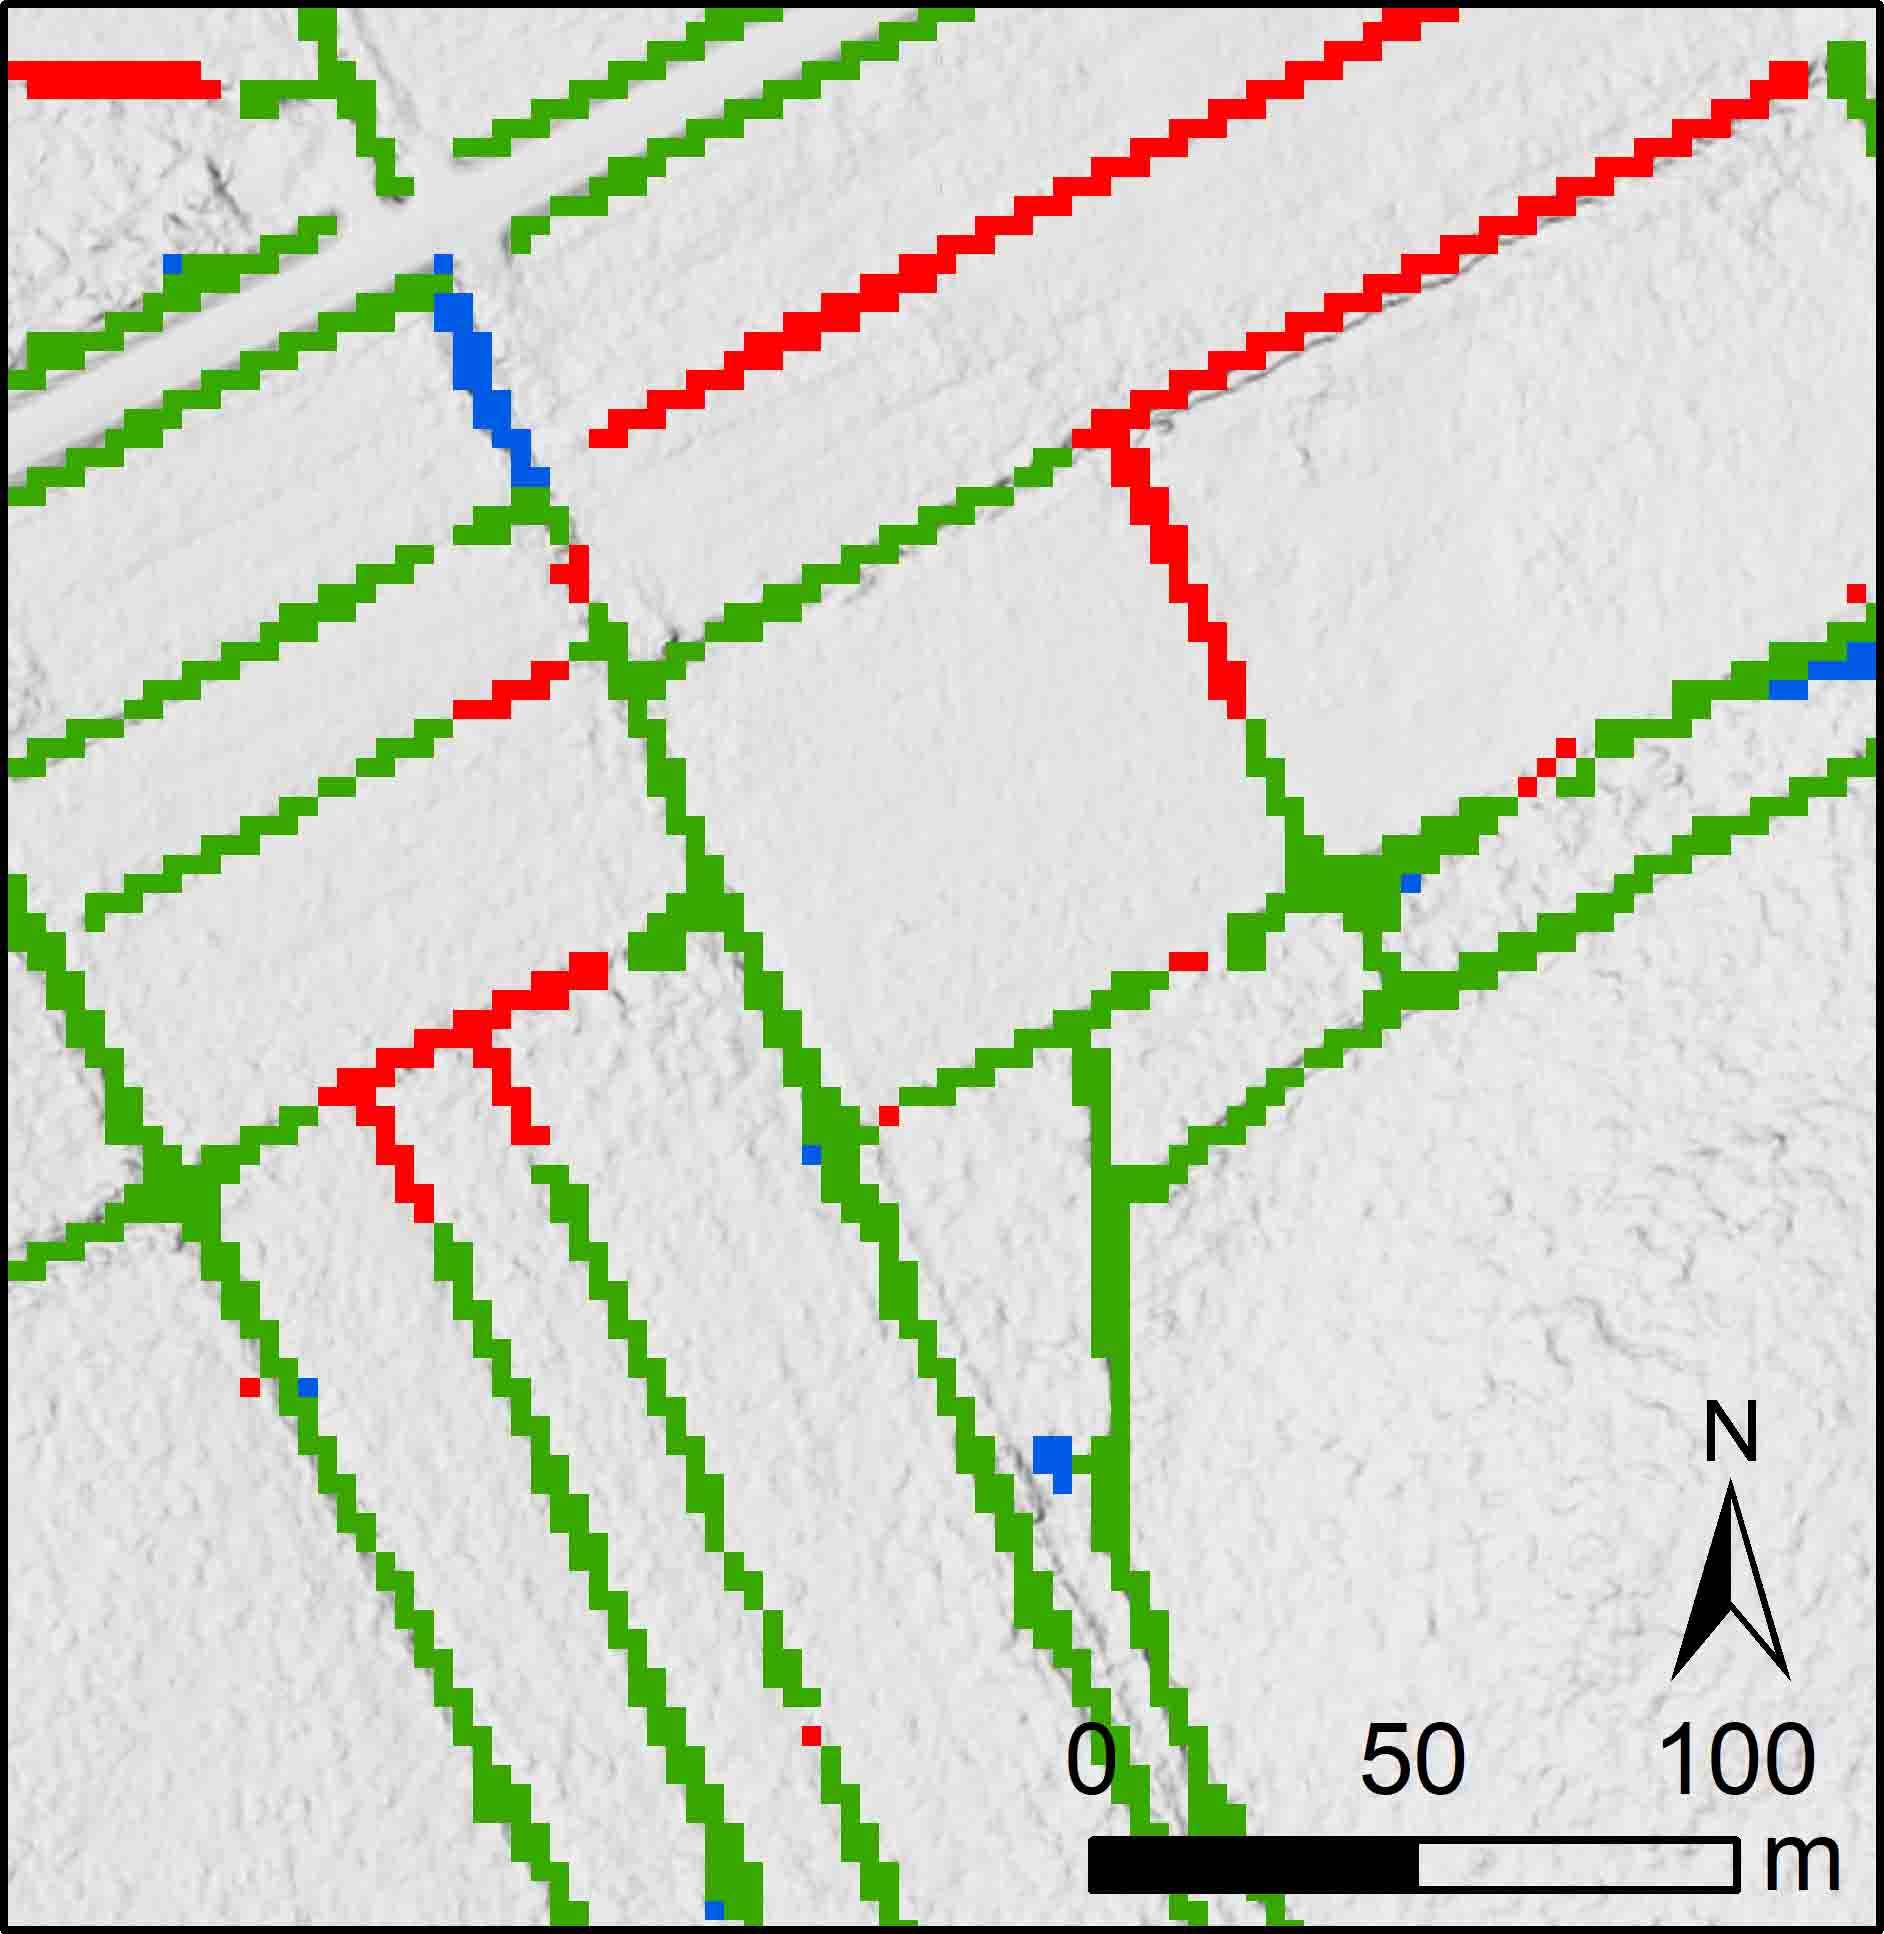
\includegraphics{./images/re_evaluation_2_lo.jpg}}}
    \caption{Illustration of the modified evaluation labels\DIFdelbeginFL \DIFdelFL{where }\textbf{\DIFdelFL{a}} %DIFAUXCMD
\DIFdelFL{shows the original result, and }\textbf{\DIFdelFL{b}} %DIFAUXCMD
\DIFdelFL{shows the modified result}\DIFdelendFL . Green marks true positives, red marks false negatives, and blue marks false positives. False positives and false negatives that lay within one grid zone (\DIFdelbeginFL \DIFdelFL{3 }\DIFdelendFL \DIFaddbeginFL \DIFaddFL{9 }\DIFaddendFL $m^2$) of a ditch label were evaluated as true positives and true negatives. \DIFaddbeginFL \textbf{\DIFaddFL{a:}} \DIFaddFL{Original results, }\textbf{\DIFaddFL{b:}} \DIFaddFL{Modified results. }\DIFaddendFL }
    \label{fig:newlabels}
\end{figure}

\section{Results and analysis}
\DIFaddbegin \DIFadd{In the national survey (NILS), a total of 1103 natural watercourses, 131 straightened watercourses/channels, and 2089 ditches were found in the field. This simple investigation highlights two things: Firstly, the ditches make up the majority of the small scale water channels in the Swedish landscape; almost twice as many as the natural streams. Secondly, most of the small scale channels are missing on the current maps; only 45 \% of the natural watercourses, 25 \% of the straightened watercourses/channels, and 9 \% of the ditches were mapped (}\hyperref[fig:watercoursebarplot]{Figure} \DIFadd{\ref{fig:watercoursebarplot}).
}\DIFaddend 

\DIFaddbegin \begin{figure}[!htb]
    \centering
    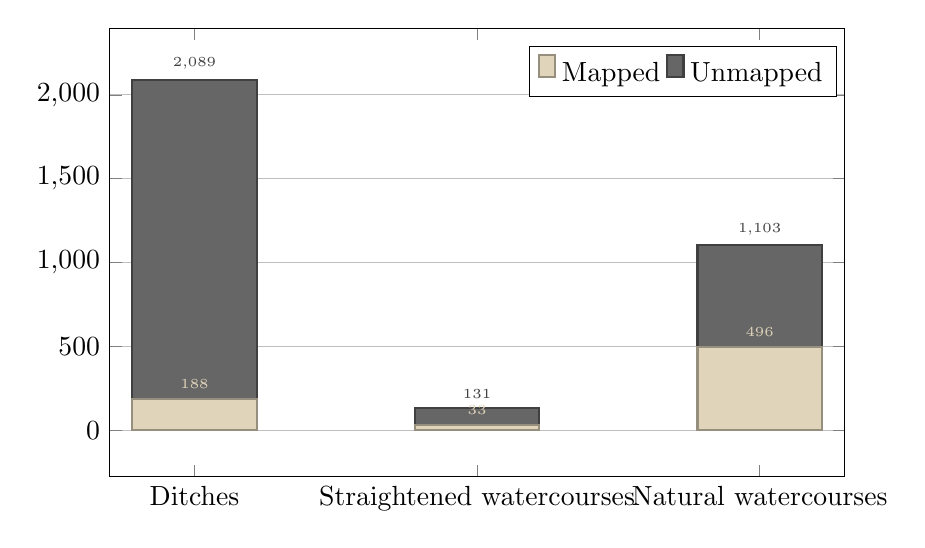
\begin{tikzpicture}
    \begin{axis}[
        width={0.9\textwidth},
        height={0.6\textwidth},
        ylabel={fluorescence},
        ybar stacked,
        ymajorgrids=true,
    	bar width=45pt,
    	nodes near coords,
    	every node near coord/.append style={font=\tiny},
        enlarge y limits={0.15},
        enlarge x limits=0.15,
        legend style={at={(0.78,0.96)},
          anchor=north,legend columns=-1},
        ylabel={{}},
        symbolic x coords={Ditches, Straightened  watercourses, Natural  watercourses},
        xtick=data,
        ytick={0,500,1000,1500,2000},
        x tick label style={rotate=0,anchor=north},
        ]
    \addplot+[ybar,color=custombeige,fill=custombeige,draw=custombeigeouter,thick] plot coordinates {(Ditches,188) (Straightened  watercourses,33) 
      (Natural  watercourses,496)};
    \addplot+[ybar,color=customgrayouter,fill=customgray,draw=customgrayouter,thick] plot coordinates {(Ditches,1901) (Straightened  watercourses,98) 
      (Natural  watercourses,607)};
    \legend{\strut Mapped, \strut Unmapped}
    \end{axis}
    \end{tikzpicture}
    \caption{\DIFaddFL{The bars indicate the number of observed channels in the National Inventory of Landscapes in Sweden's (NILS) line inventory of small watercourses (width $<$ 6 m). The colours of the bars indicate if they are mapped or not on the Swedish Property map.}}
    \label{fig:watercoursebarplot}
\end{figure}



\DIFaddend \hyperref[recreatedpredictionperformance]{Table} \ref{recreatedpredictionperformance} shows the evaluation metrics from the experiments with the digital terrain indices separately. Of the four, the Impoundment Index and the HPMF index performed relatively close to each other and outperformed the other indices for most of the metrics.

\begin{table}[!htb]
    \tbl{Metrics from the total results of the four digital terrain indices experiments.}
    {\begin{tabular}{lcccc} \toprule
        Metric & Sky View Factor & Impoundment & HPMF & Slope\\ \midrule
        Accuracy \%     & 83.67 & 97.07 & 97.45 & 82.66 \\
        Recall \%       & 44.54 & 29.98 & 25.31 & 34.83 \\
        Precision \%    &{ 4.00}  & 18.51 & 20.10 & { 2.99} \\
        $\kappa$ rating & 0.048 & 0.215 & 0.211 & 0.029 \\
        AUPRC & 0.247 & 0.248 & 0.232 & 0.194 \\ \bottomrule
    \end{tabular}}
    \label{recreatedpredictionperformance}
\end{table}

\hyperref[predictionperformance]{Table} \ref{predictionperformance} displays all the evaluation metrics for the prediction of our method. The confidence intervals were calculated from the 11 different subsections that the experiment was performed on. Because the subsections have varying amounts of ditches in them, the confidence intervals will not be completely accurate, but will produce a close estimation.

From \hyperref[predictionperformance]{Table} \ref{predictionperformance}, it \DIFdelbegin \DIFdel{can be seen }\DIFdelend \DIFaddbegin \DIFadd{is observed }\DIFaddend that averaging the results from the 11 subsections \DIFdelbegin \DIFdel{will }\DIFdelend \DIFaddbegin \DIFadd{would }\DIFaddend yield a very similar value to the total results, indicating that the \DIFdelbegin \DIFdel{model }\DIFdelend \DIFaddbegin \DIFadd{ditch detector }\DIFaddend generally performs equally well on subsections with a small amount of ditches as on subsections with a large amount of ditches.

\begin{table}[!htb]
    \DIFdelbeginFL %DIFDELCMD < \tbl{Metrics for the prediction performance of our model.}{\begin{tabular}{lccc} 
%DIFDELCMD <         \toprule
%DIFDELCMD <         Metric & Total\textsuperscript{a} & Subsection\textsuperscript{b}& CI 95\%\textsuperscript{c} \\ 
%DIFDELCMD <         &&Average&\\ \midrule
%DIFDELCMD <         Accuracy     \% & 98.96 & 98.96 & [98.64 , 99.27] \\
%DIFDELCMD <         Recall       \% & 77.41 & 76.81 & [69.35 , 84.27] \\
%DIFDELCMD <         Precision    \% & 73.89 & 73.06 & [69.73 , 76.40] \\
%DIFDELCMD <         $\kappa$ rating & 0.751 & 0.739 & [0.693 , 0.786] \\
%DIFDELCMD <         AUPRC           & 0.759 & 0.752 & [0.706 , 0.798] \\ 
%DIFDELCMD <         \bottomrule
%DIFDELCMD <     \end{tabular}}
%DIFDELCMD <     %%%
\DIFdelendFL \DIFaddbeginFL \tbl{Metrics for the prediction performance of our ditch detector.}{\begin{tabular}{lccc} 
        \toprule
        Metric & Total\textsuperscript{a} & Subsection\textsuperscript{b}& CI 95\%\textsuperscript{c} \\ 
        &&Average&\\ \midrule
        Accuracy     \% & 99.00 & 99.00 & [98.69 , 99.32] \\
        Recall       \% & 70.28 & 70.19 & [61.28 , 79.09] \\
        Precision    \% & 77.38 & 75.79 & [71.94 , 79.64] \\
        $\kappa$ rating & 0.732 & 0.718 & [0.655 , 0.781] \\
        AUPRC           & 0.741 & 0.733 & [0.674 , 0.791] \\ 
        \bottomrule
    \end{tabular}}
    \DIFaddendFL \tabnote{
        \textsuperscript{a} The result of all 11 subsection experiments when combined. \newline
        \textsuperscript{b} An average score from the 11 different subsections that the experiment was performed on. \newline
        \textsuperscript{c} Confidence intervals at 95 \% confidence level.}
    \label{predictionperformance}
\end{table}

The $\kappa$ rating for our method can be seen in the \textit{Total} column in \hyperref[predictionperformance]{Table} \ref{predictionperformance} ($\kappa$ = \DIFdelbegin \DIFdel{0.751}\DIFdelend \DIFaddbegin \DIFadd{0.732}\DIFaddend ). The $\kappa$ ratings from the four digital terrain indices experiments can be seen in  \hyperref[recreatedpredictionperformance]{Table} \ref{recreatedpredictionperformance} ($\kappa$ = 0.048, $\kappa$ = 0.215, $\kappa$ = 0.211, $\kappa$ = 0.029). Because the $\kappa$ rating from our method outperforms all digital terrain indices, our hypothesis \DIFaddbegin \DIFadd{that combining digital terrain indices with a machine learning produces better ditch detection than using single terrain indices }\DIFaddend has been confirmed by the experiments. Most false positives lie in stream channels (\hyperref[fig:resultsillustrations]{Figure} \ref{fig:resultsillustrations} \hyperref[fig:resultsillustrations]{a, b}) and most false negatives occurred either due to ditches being too shallow (\hyperref[fig:resultsillustrations]{Figure} \ref{fig:resultsillustrations} \hyperref[fig:resultsillustrations]{c, d}), or due to the attempt at removing streams using the input variables as explained in \ref{impoundmentstreamremoval} removing the deepest ditches  (\hyperref[fig:resultsillustrations]{Figure} \ref{fig:resultsillustrations} \hyperref[fig:resultsillustrations]{e, f}).

\begin{figure} [!htb]
    \centering
    \subfigure[]{
        \resizebox*{5.5cm}{!}{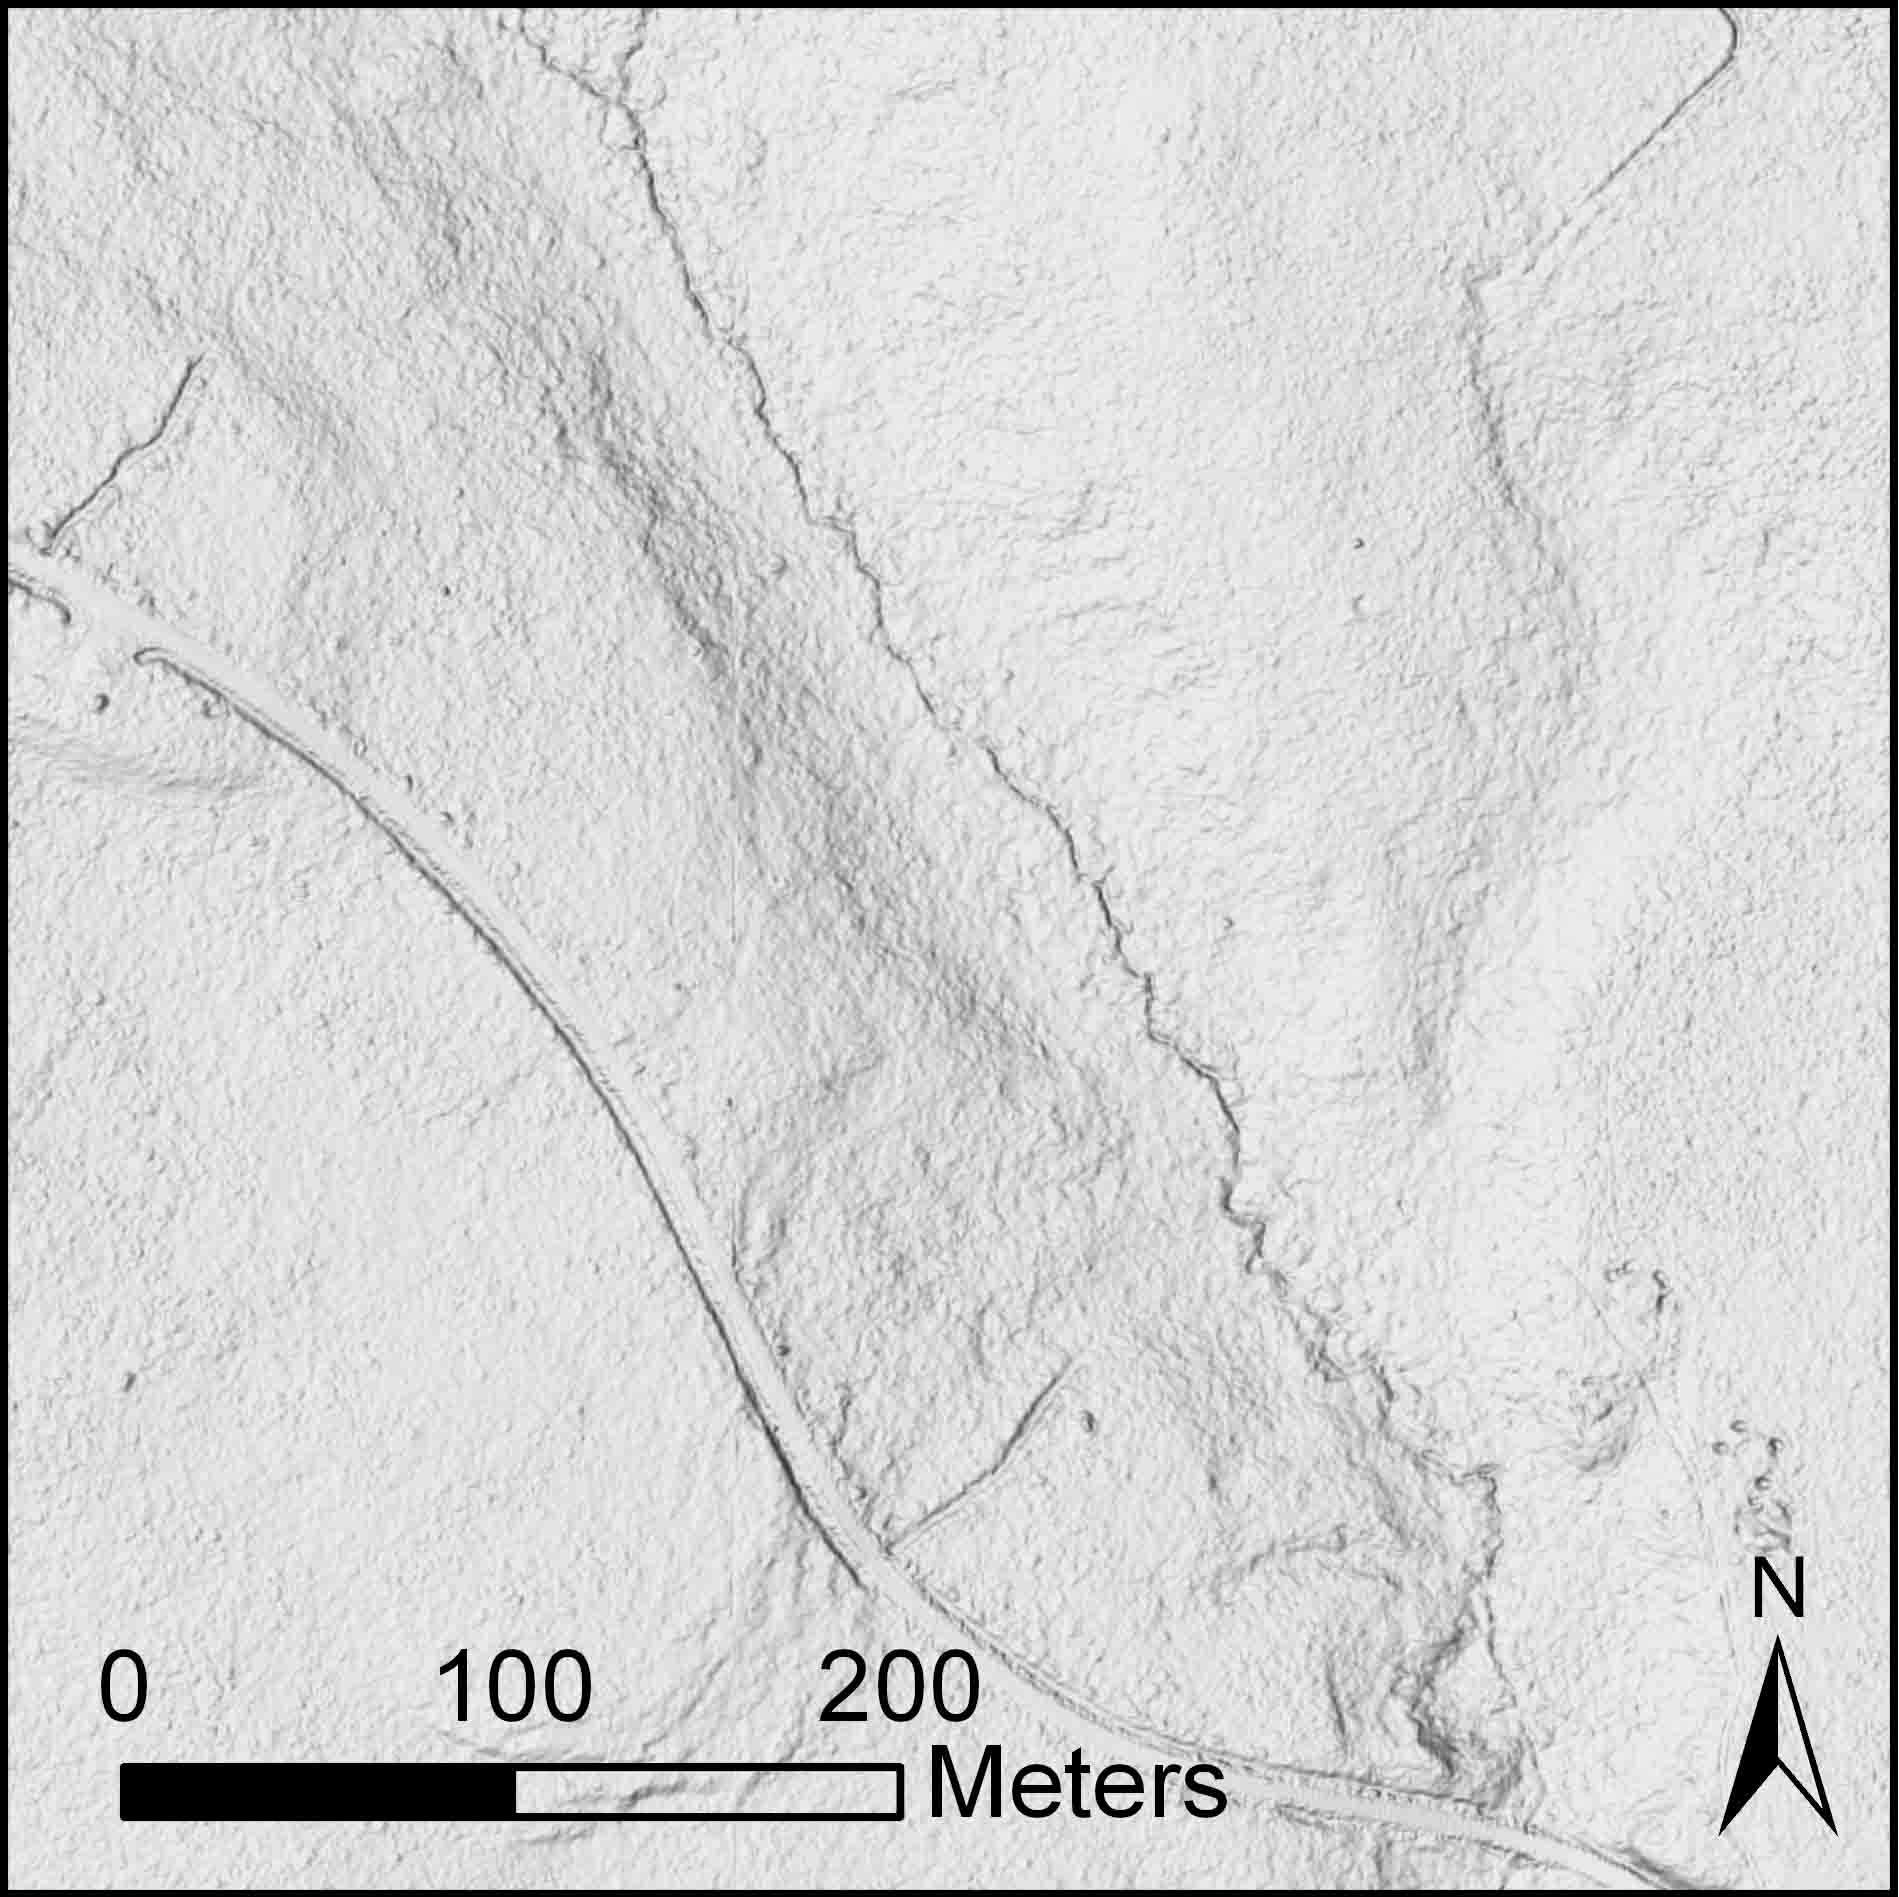
\includegraphics{./images/results_illustration_1_lo.jpg}}}\hspace{5pt}
    \subfigure[]{
        \resizebox*{5.5cm}{!}{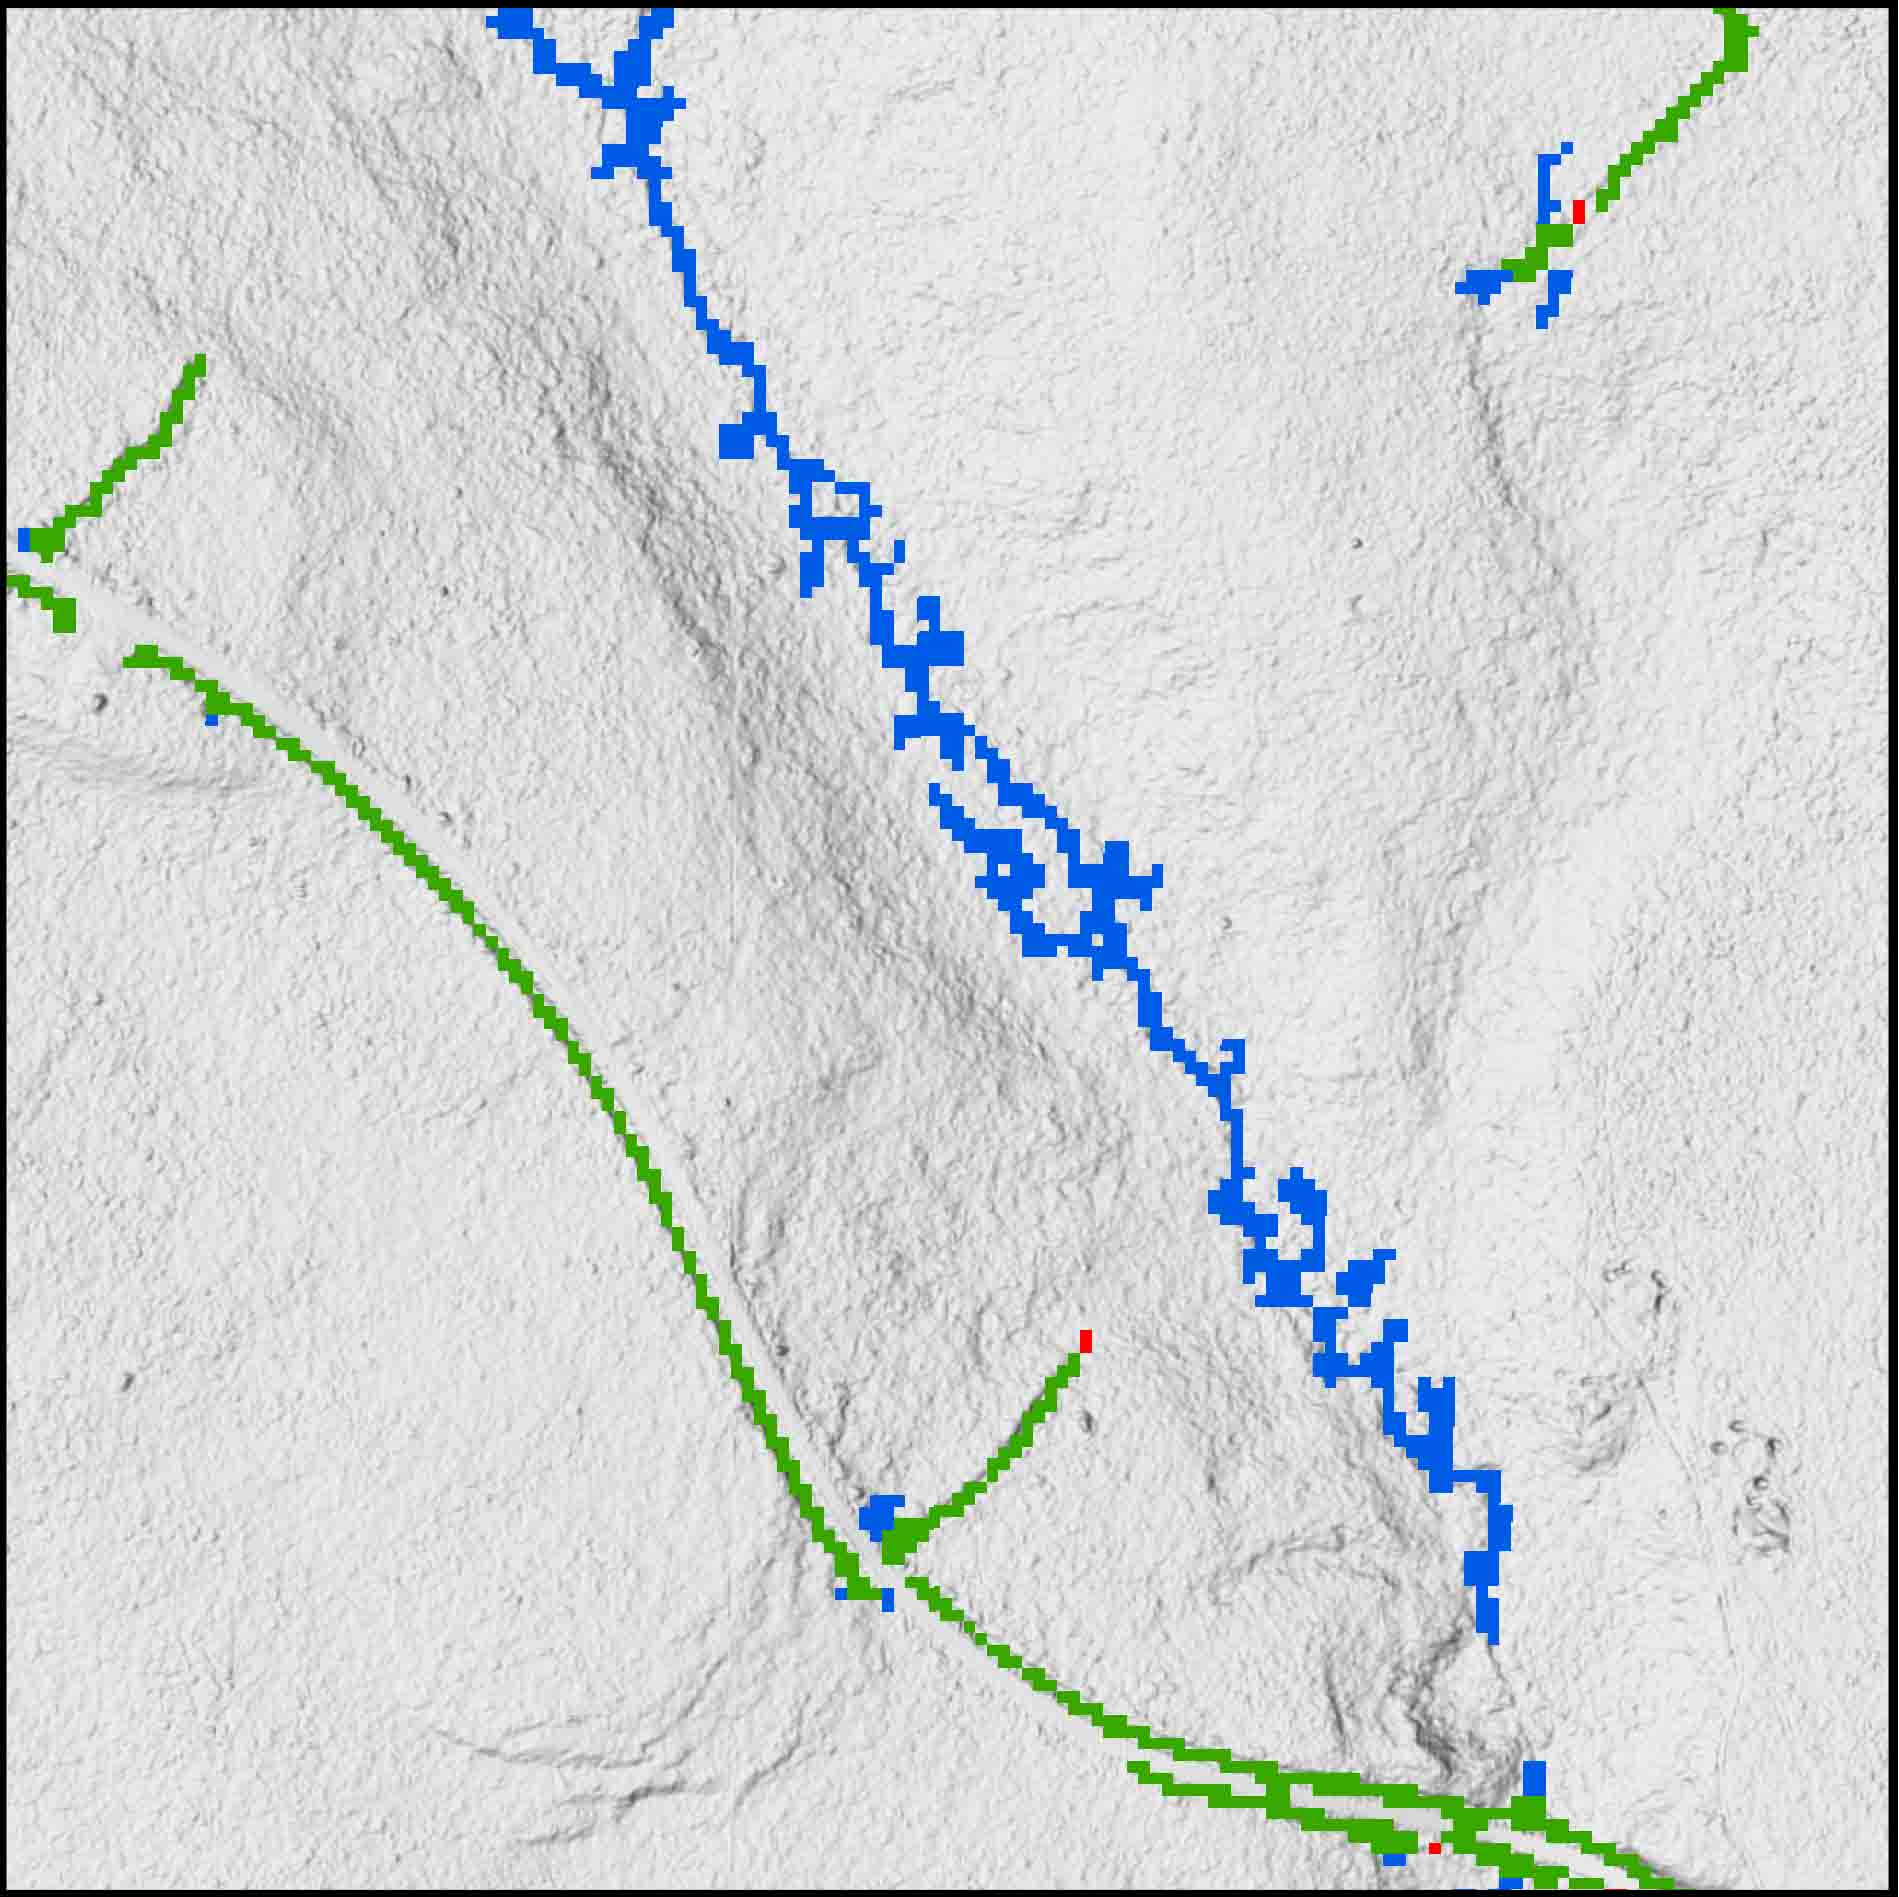
\includegraphics{./images/results_illustration_2_lo.jpg}}}
    \subfigure[]{
        \resizebox*{5.5cm}{!}{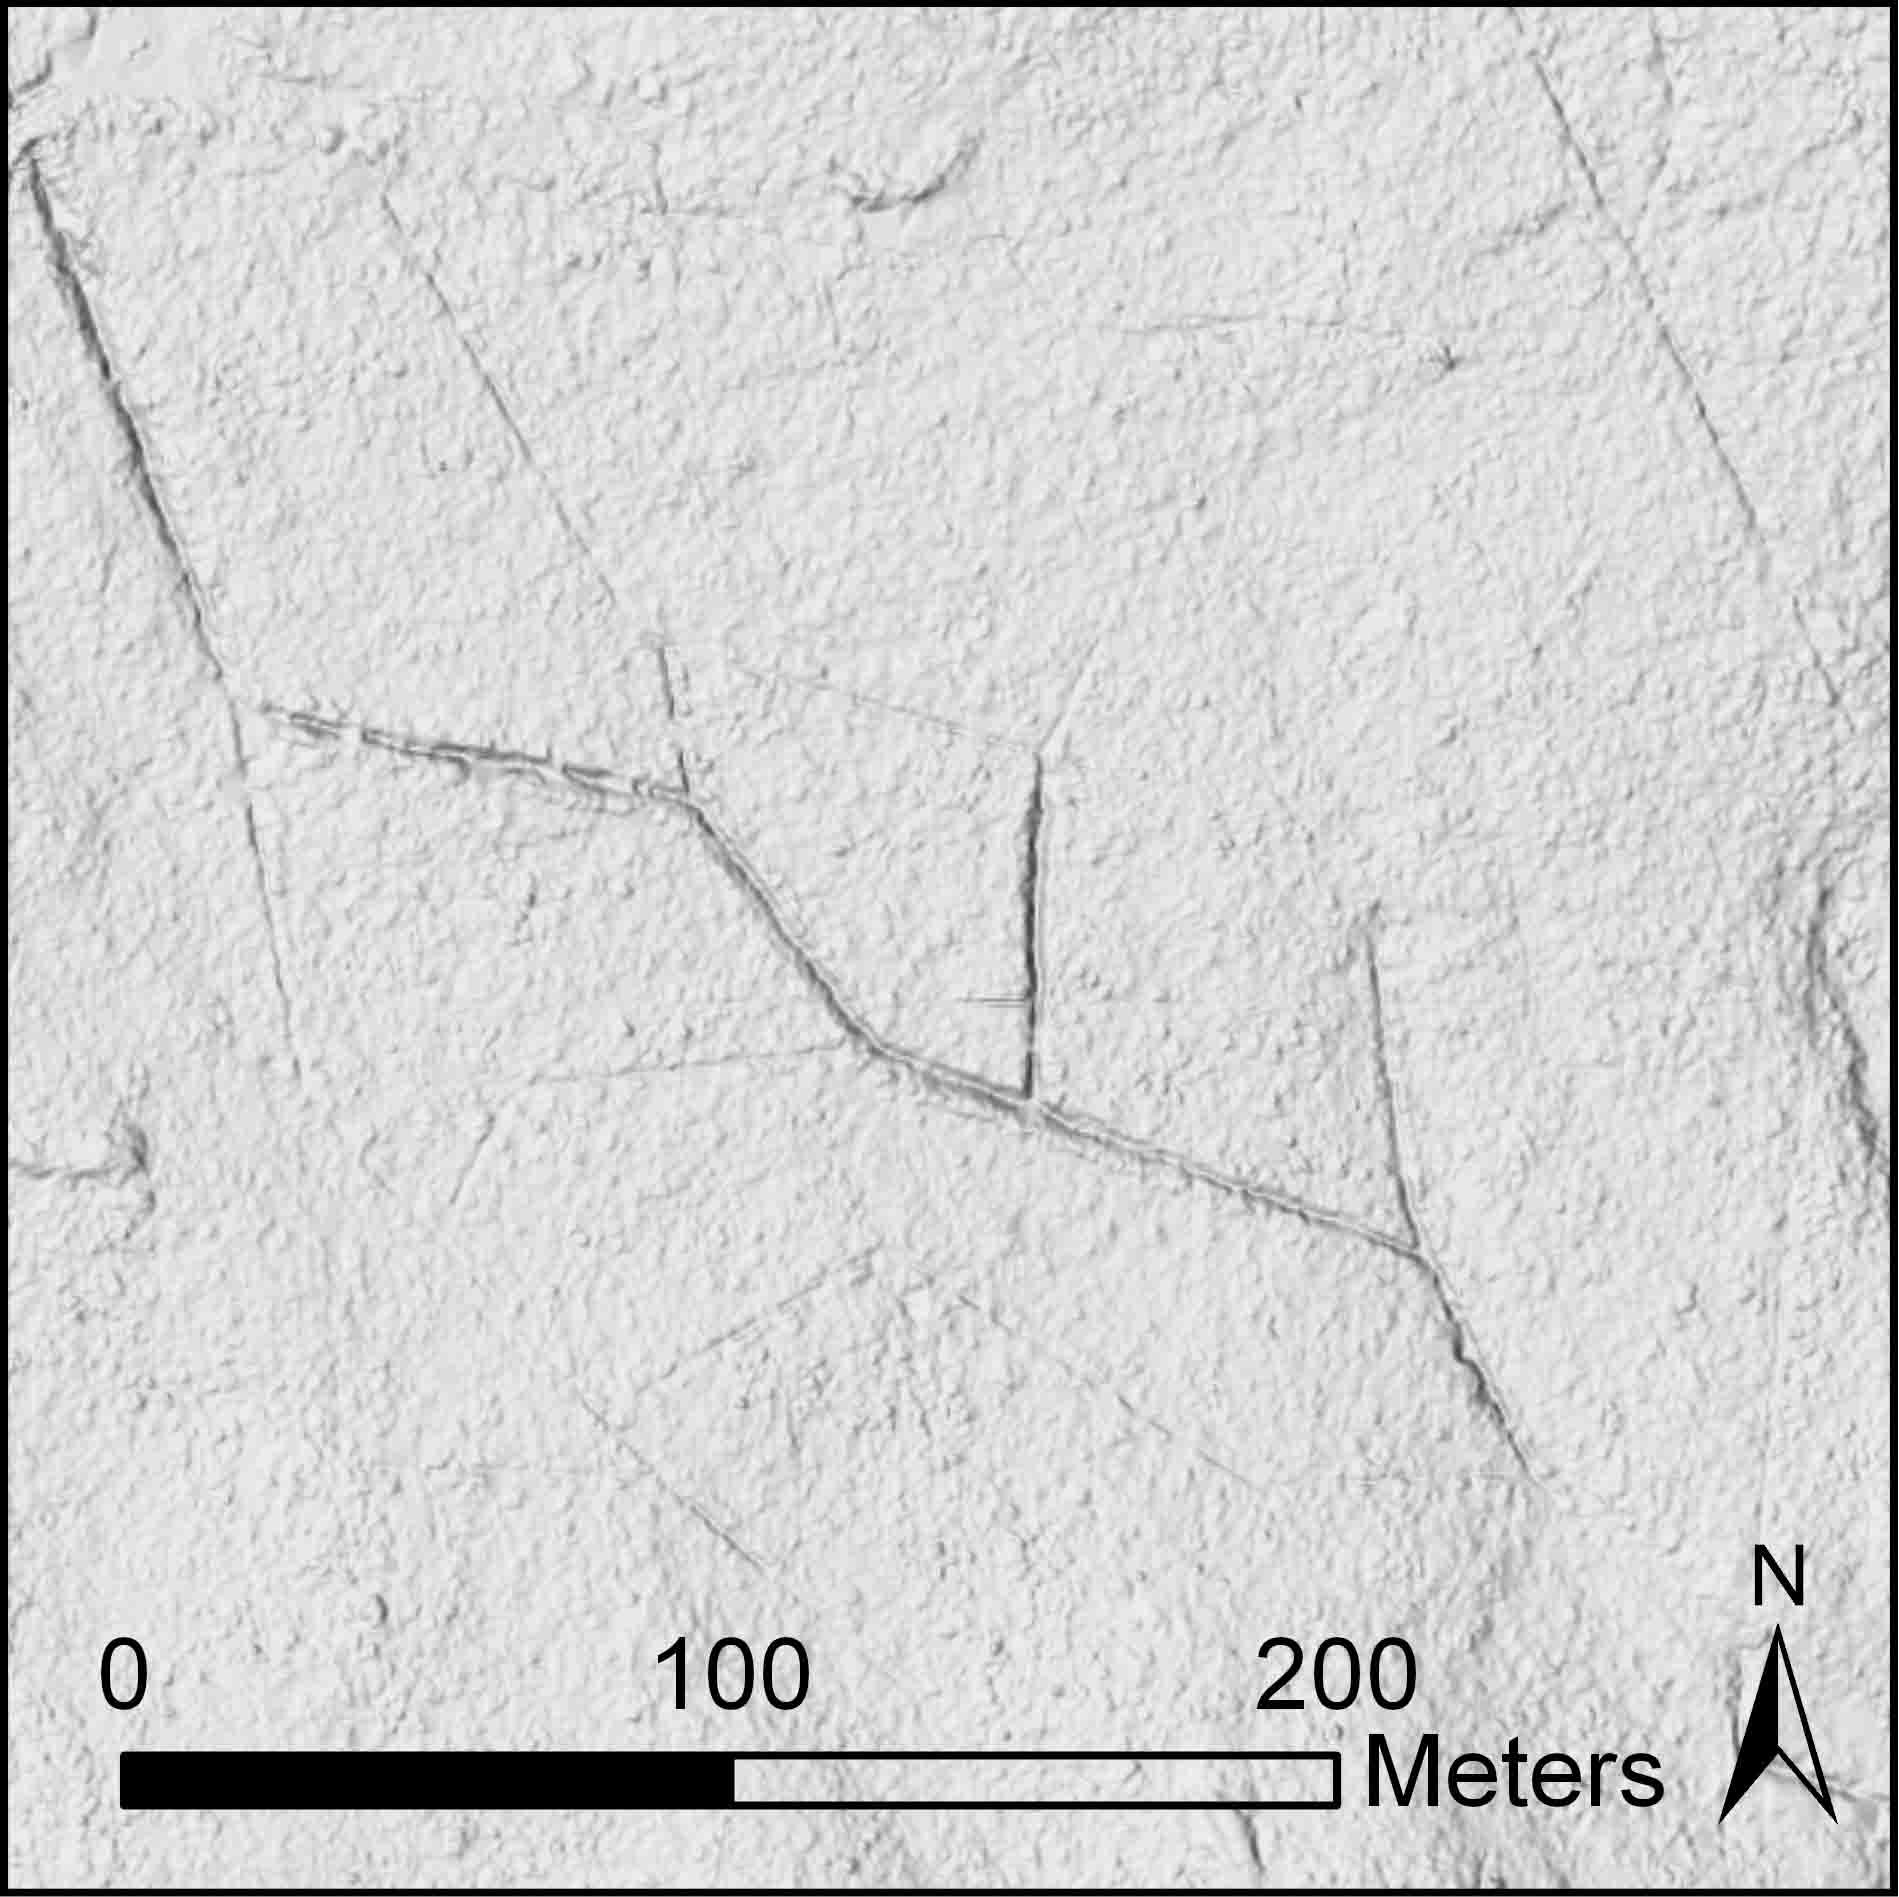
\includegraphics{./images/results_illustration_3_lo.jpg}}}\hspace{5pt}
    \subfigure[]{
        \resizebox*{5.5cm}{!}{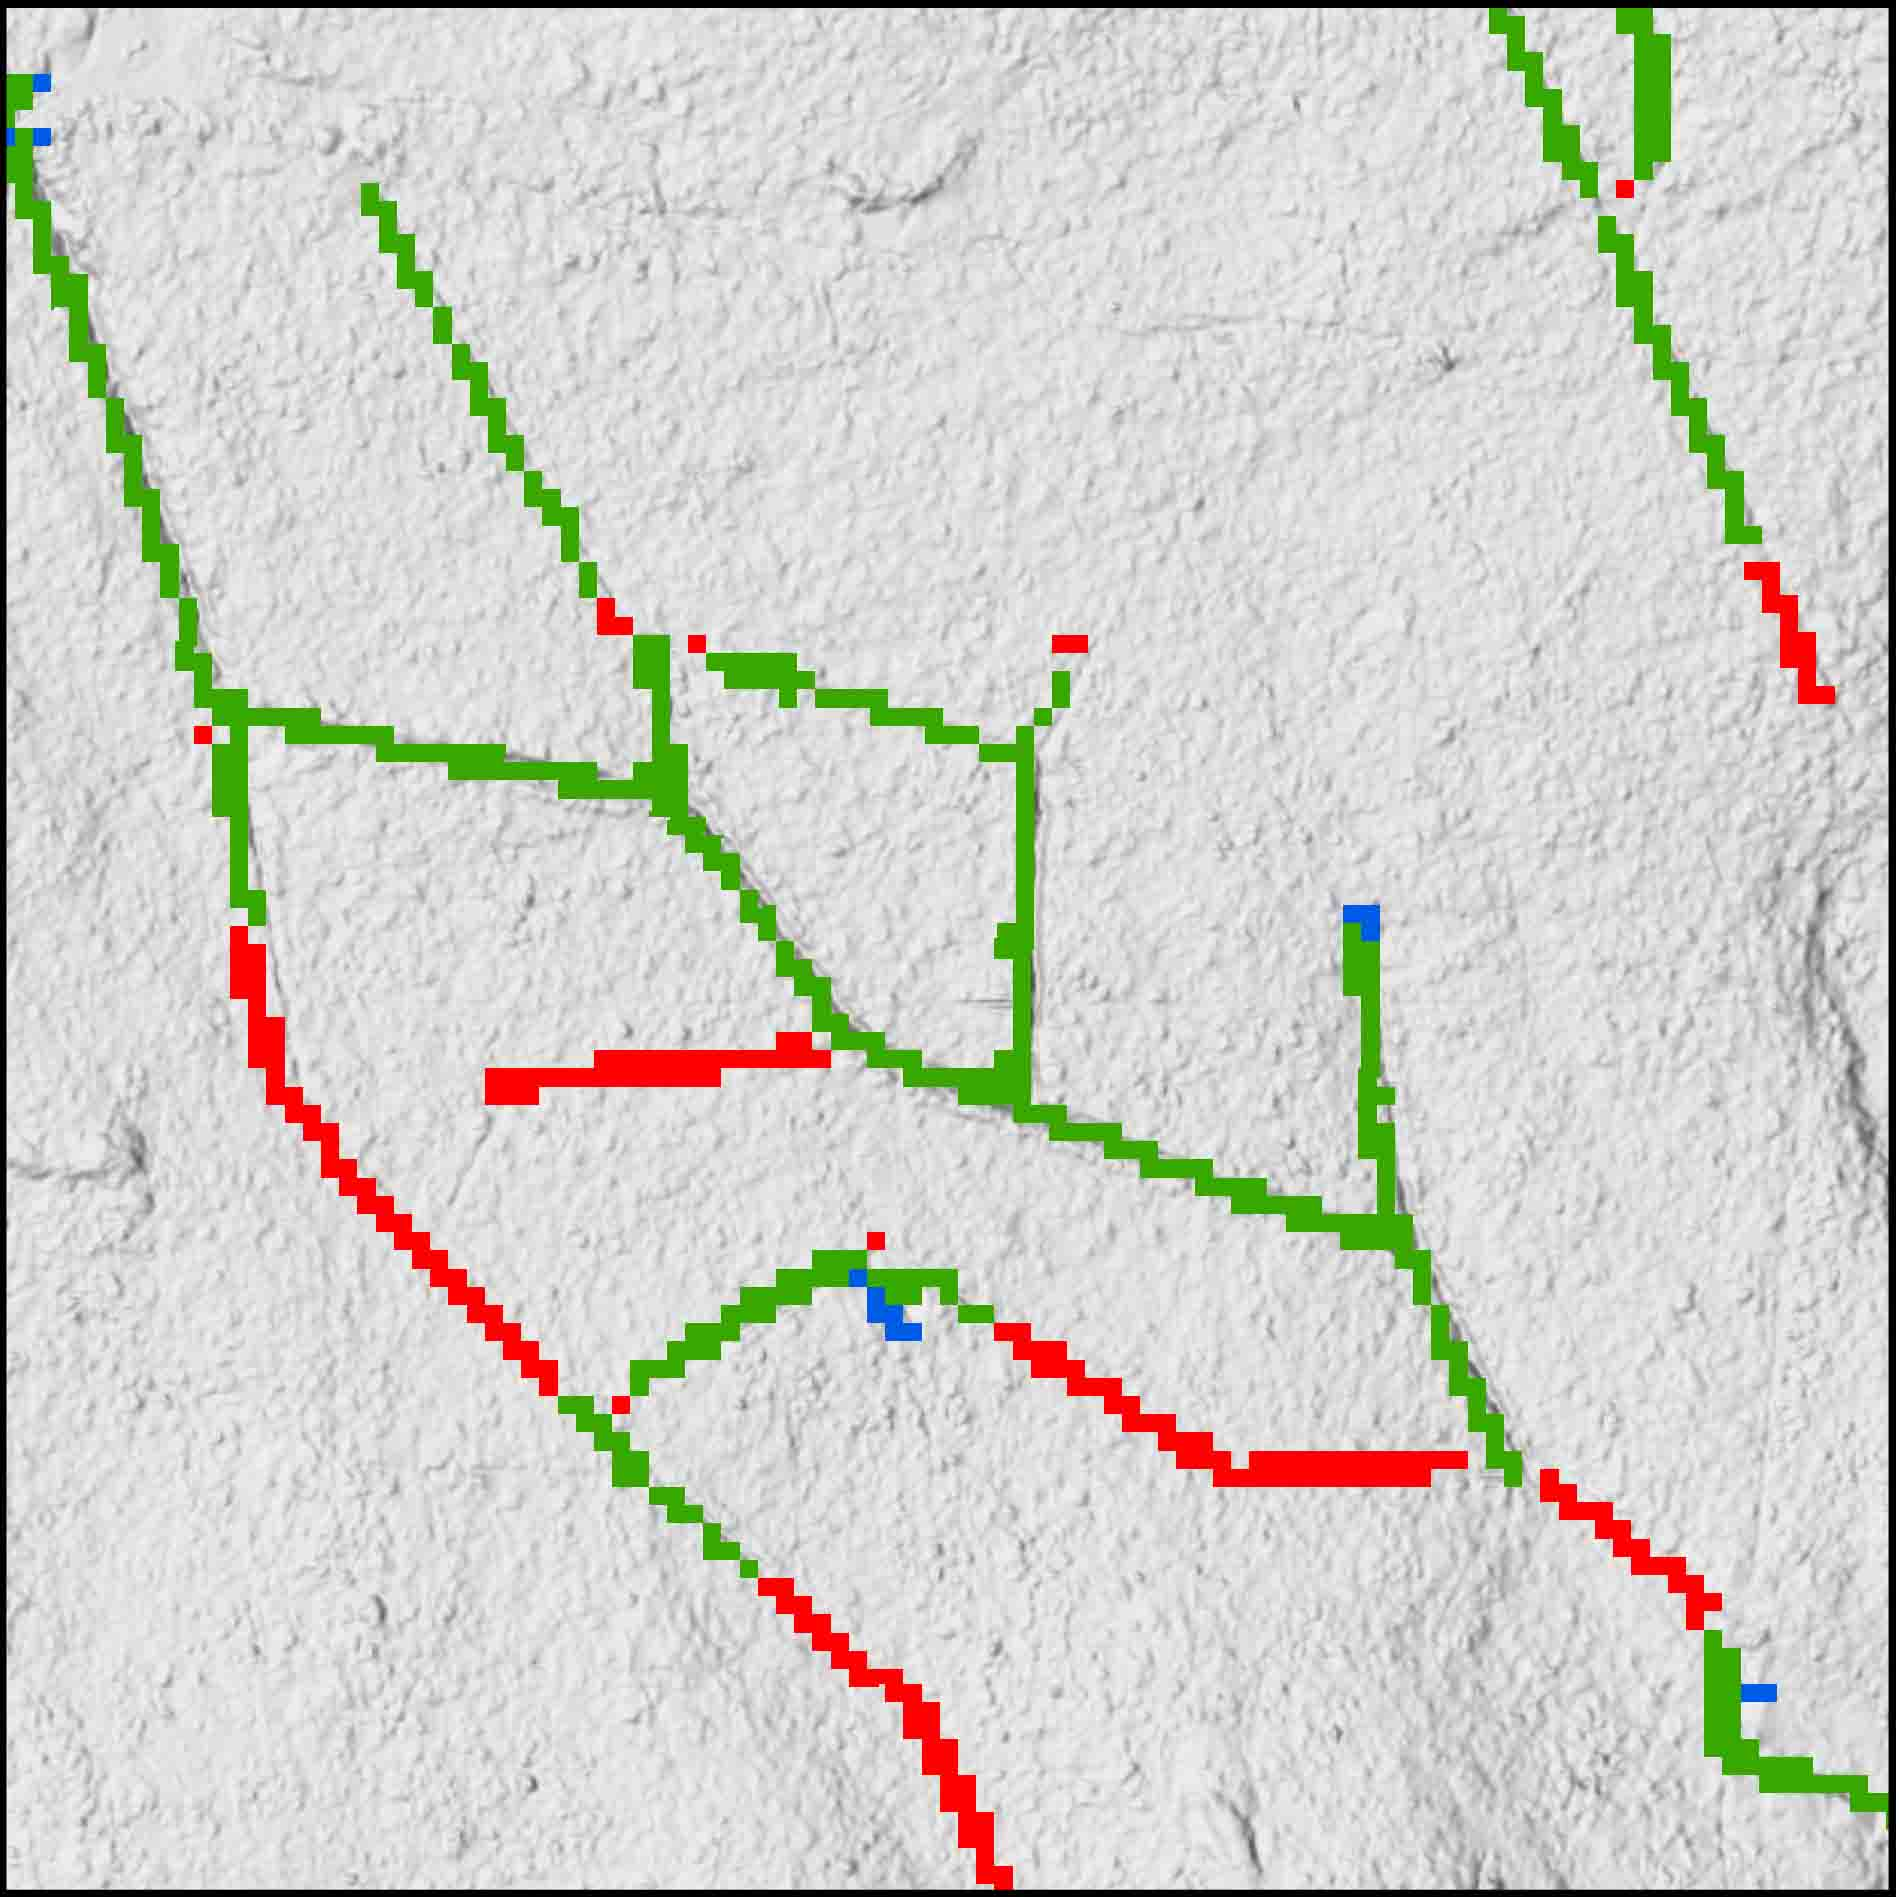
\includegraphics{./images/results_illustration_4_lo.jpg}}}
    \subfigure[]{
        \resizebox*{5.5cm}{!}{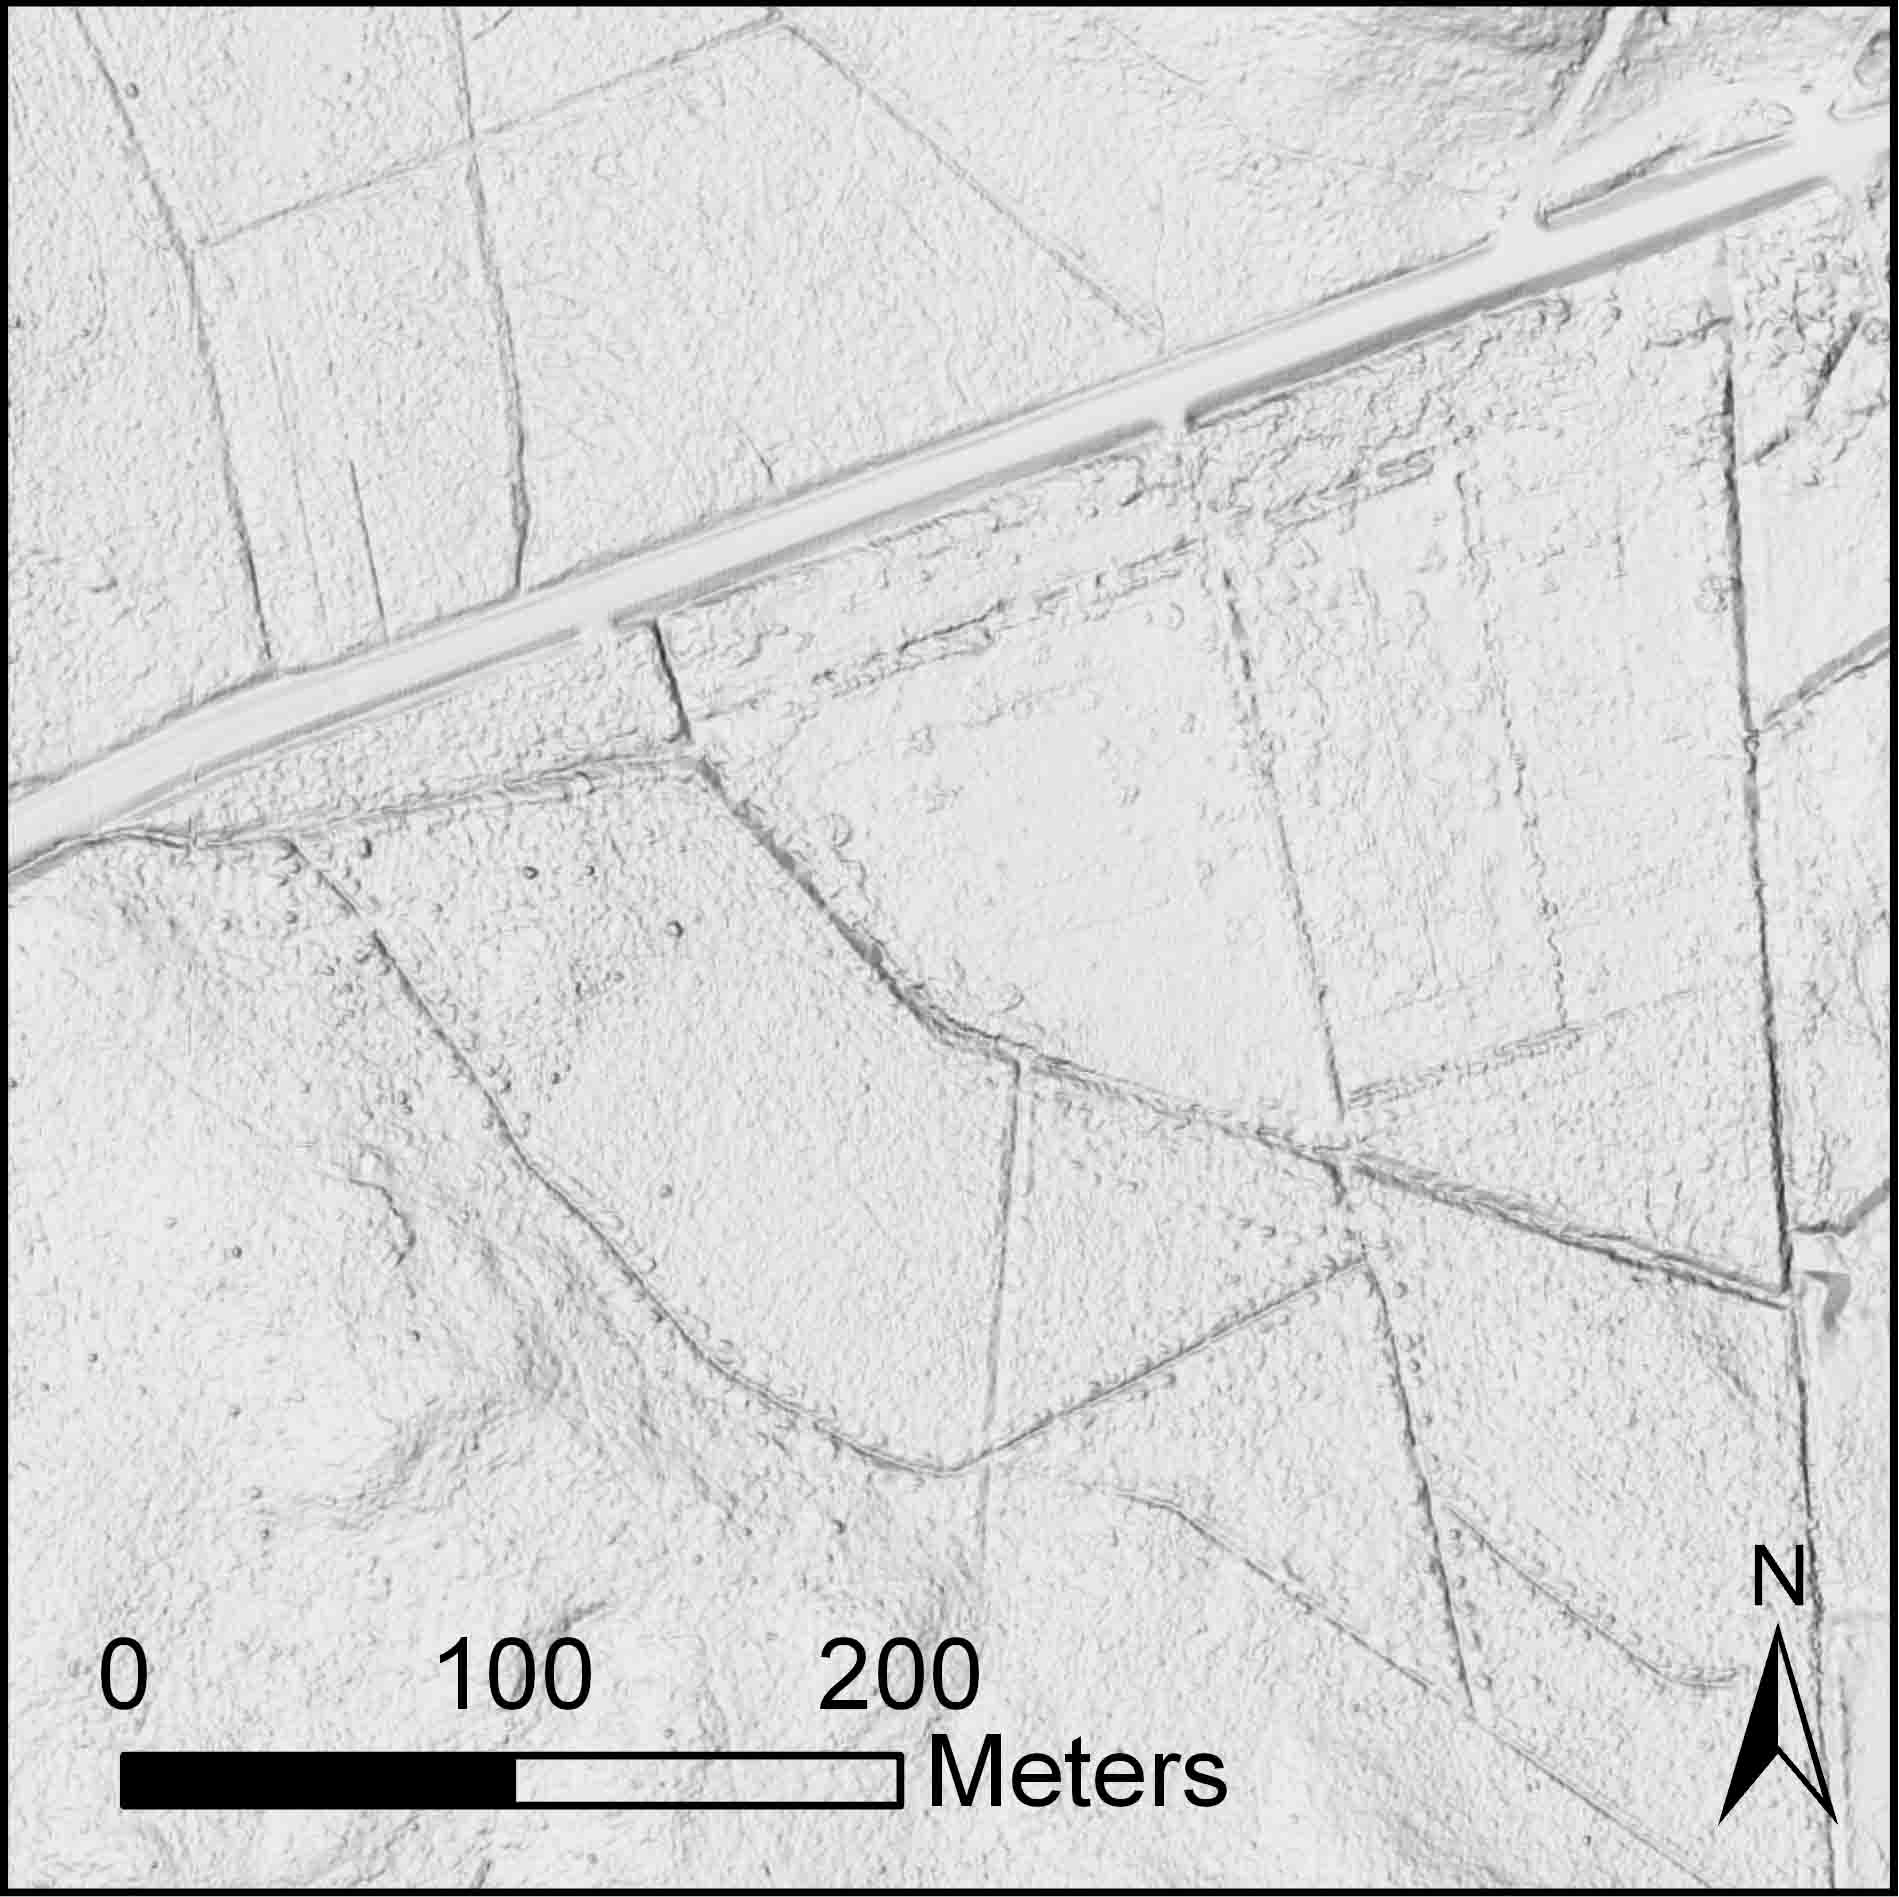
\includegraphics{./images/results_illustration_5_lo.jpg}}}\hspace{5pt}
    \subfigure[]{
        \resizebox*{5.5cm}{!}{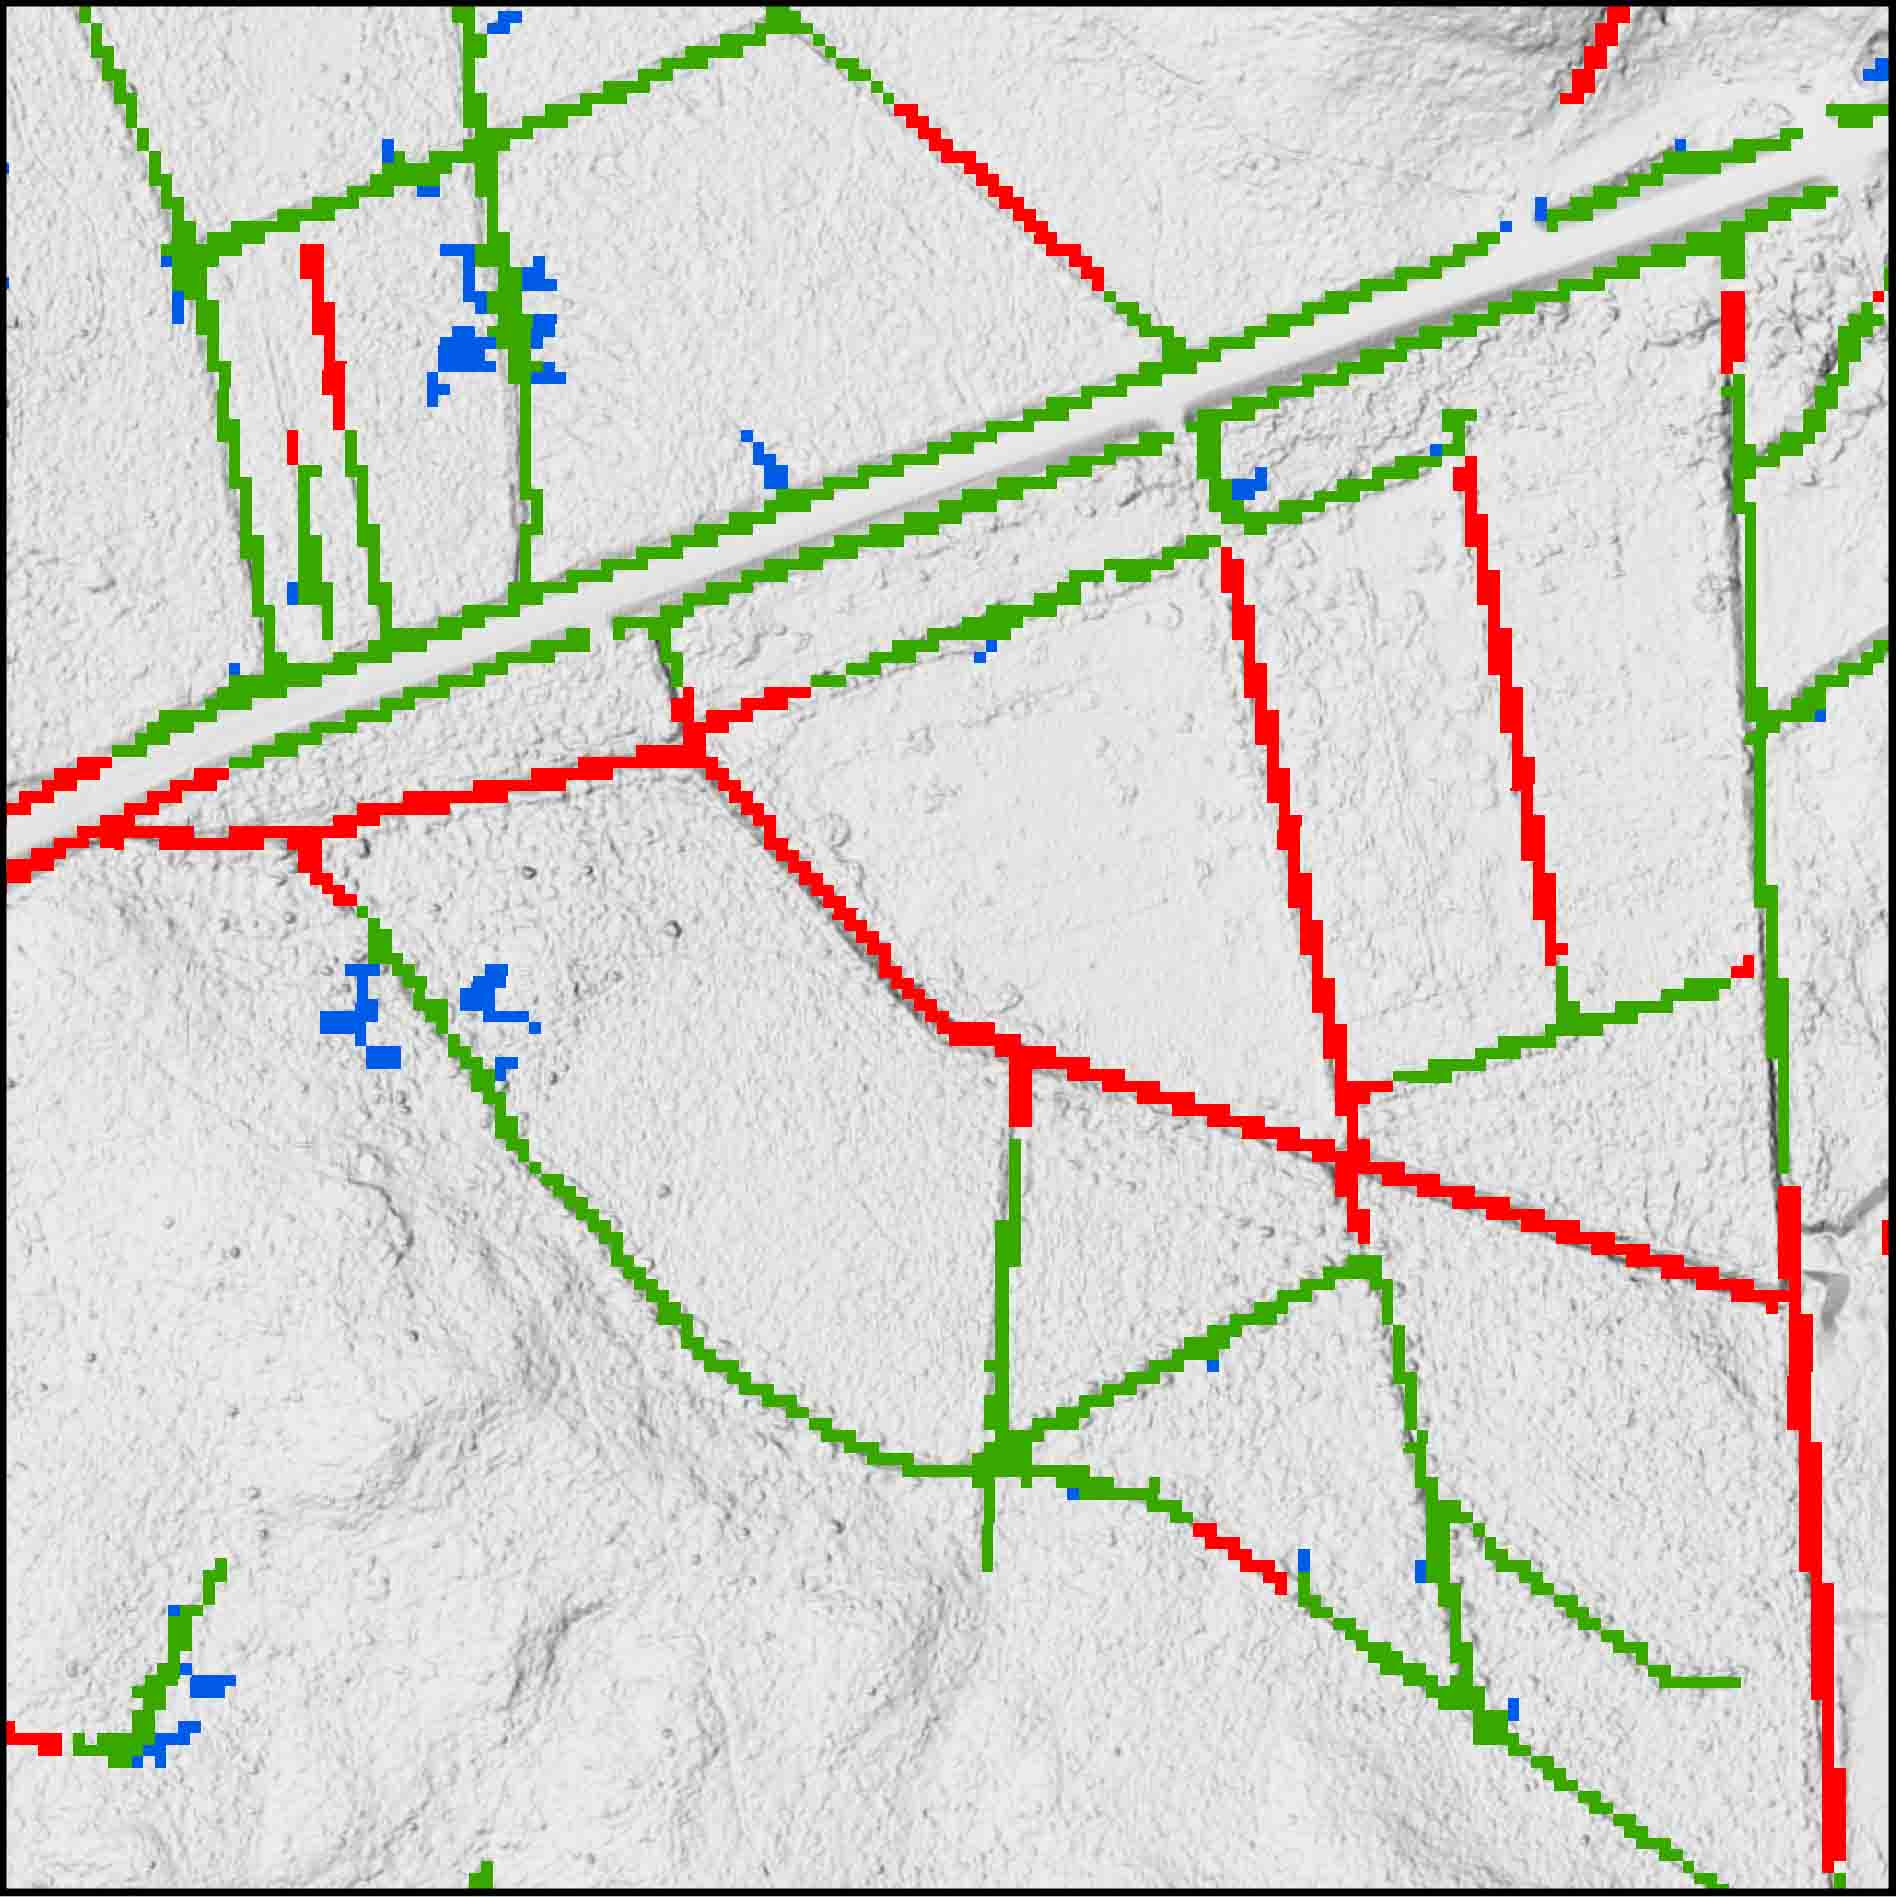
\includegraphics{./images/results_illustration_6_lo.jpg}}}
    \caption{The left panel shows the hillshade for a number of subsections, and the right panel shows the hillshade with the extracted ditches superimposed on top. Green marks correctly classified ditches (true positives), red marks missed ditches (false negatives), blue marks incorrectly classified ditches (false positives), and transparent areas mark correctly classified non-ditches (true negatives). \textbf{a} and \textbf{b} illustrate that the most common false positives were natural stream channels being classified as ditches. \textbf{c} and \textbf{d} illustrate that very shallow ditches that were barely visible in the DEM were not captured with our \DIFdelbeginFL \DIFdelFL{model}\DIFdelendFL \DIFaddbeginFL \DIFaddFL{ditch detector}\DIFaddendFL . \textbf{e} and \textbf{f} illustrate that some of the deepest and more prominent ditches were also missed. This occurred as a result of attempting to get rid of more false positives in the form of streams by using the input variables, as explained in \ref{impoundmentstreamremoval}.}
    \label{fig:resultsillustrations}
\end{figure}
\clearpage

In \hyperref[featureimportancetable]{Table} \ref{featureimportancetable}, the top 20 \DIFaddbegin \DIFadd{(out of 40) }\DIFaddend input variables from the Random Forests \DIFdelbegin \DIFdel{model }\DIFdelend \DIFaddbegin \DIFadd{models }\DIFaddend are presented with their importance percentages for the \DIFdelbegin \DIFdel{model }\DIFdelend \DIFaddbegin \DIFadd{models }\DIFaddend making a successful prediction. \DIFdelbegin \DIFdel{From the table, it can be seen that input }\DIFdelend \DIFaddbegin \DIFadd{Input }\DIFaddend variables based on HPMF and Impoundment Index contributed the most to a successful prediction. The Gini importance was obtained using the Gini impurity for each variable \citep{gini}.

\begin{table} [!htb]
    \DIFdelbeginFL %DIFDELCMD < \tbl{The top 20 input variables (out of 81) by importance when the model makes a prediction.}
%DIFDELCMD <         %%%
        \DIFaddendFL {
        \caption{The top 20 input variables (out of 40) by importance when the models make a prediction.}
        \resizebox{\linewidth}{!}{%
        
        \begin{tabular}{llr}
          \toprule
          Position & Variable\textsuperscript{a} & Importance (\%) \\ \midrule
          1.  & Impoundment mean 3                                  & \DIFdelbeginFL \DIFdelFL{11.08}\DIFdelendFL \DIFaddbeginFL \DIFaddFL{7.33}\DIFaddendFL \\
          2.  & \DIFdelbeginFL \DIFdelFL{Impoundment }\DIFdelendFL \DIFaddbeginFL \DIFaddFL{HPMF }\DIFaddendFL mean 4                                         & \DIFdelbeginFL \DIFdelFL{7.44}\DIFdelendFL \DIFaddbeginFL \DIFaddFL{6.23}\DIFaddendFL \\
          3.  & \DIFdelbeginFL \DIFdelFL{HPMF }\DIFdelendFL \DIFaddbeginFL \DIFaddFL{Impoundment }\DIFaddendFL mean 4                                  & \DIFdelbeginFL \DIFdelFL{7.03}\DIFdelendFL \DIFaddbeginFL \DIFaddFL{5.57}\DIFaddendFL \\
          4.  & \DIFdelbeginFL \DIFdelFL{HPMF mean 3                                         }\DIFdelendFL \DIFaddbeginFL \DIFaddFL{Impoundment mean 2                                  }\DIFaddendFL & \DIFdelbeginFL \DIFdelFL{3.97}\DIFdelendFL \DIFaddbeginFL \DIFaddFL{5.41}\DIFaddendFL \\
          5.  & \DIFdelbeginFL \DIFdelFL{Impoundment median 4                                }\DIFdelendFL \DIFaddbeginFL \DIFaddFL{HPMF mean 3                                         }\DIFaddendFL & \DIFdelbeginFL \DIFdelFL{2.97}\DIFdelendFL \DIFaddbeginFL \DIFaddFL{4.33}\DIFaddendFL \\
          6.  & Impoundment \DIFdelbeginFL \DIFdelFL{mean 2                                  }\DIFdelendFL \DIFaddbeginFL \DIFaddFL{median 4                                }\DIFaddendFL & \DIFdelbeginFL \DIFdelFL{2.53}\DIFdelendFL \DIFaddbeginFL \DIFaddFL{3.84}\DIFaddendFL \\
          7.  & \DIFdelbeginFL \DIFdelFL{Sky View Factor }\DIFdelendFL \DIFaddbeginFL \DIFaddFL{HPMF }\DIFaddendFL Gabor - streams removed                        & \DIFdelbeginFL \DIFdelFL{2.03}\DIFdelendFL \DIFaddbeginFL \DIFaddFL{3.54}\DIFaddendFL \\
          8.  & \DIFdelbeginFL \DIFdelFL{Impoundment ditch amplification                     }\DIFdelendFL \DIFaddbeginFL \DIFaddFL{HPMF median 4                                       }\DIFaddendFL & \DIFdelbeginFL \DIFdelFL{1.91}\DIFdelendFL \DIFaddbeginFL \DIFaddFL{3.40}\DIFaddendFL \\
          9.  & \DIFdelbeginFL \DIFdelFL{HPMF median 4                                       }\DIFdelendFL \DIFaddbeginFL \DIFaddFL{Impoundment median 2                                }\DIFaddendFL & \DIFdelbeginFL \DIFdelFL{1.90}\DIFdelendFL \DIFaddbeginFL \DIFaddFL{3.01}\DIFaddendFL \\
          10. & \DIFdelbeginFL \DIFdelFL{Impoundment ditch amplification }\DIFdelendFL \DIFaddbeginFL \DIFaddFL{Sky View Factor Gabor }\DIFaddendFL - streams removed             & \DIFdelbeginFL \DIFdelFL{1.76}\DIFdelendFL \DIFaddbeginFL \DIFaddFL{2.84}\DIFaddendFL \\
          11. & \DIFdelbeginFL \DIFdelFL{Slope standard deviation }\DIFdelendFL \DIFaddbeginFL \DIFaddFL{HPMF mean }\DIFaddendFL 6                                         & \DIFdelbeginFL \DIFdelFL{1.62}\DIFdelendFL \DIFaddbeginFL \DIFaddFL{2.73}\DIFaddendFL \\
          12. & \DIFdelbeginFL \DIFdelFL{Sky View Factor non-ditch amplification             }\DIFdelendFL \DIFaddbeginFL \DIFaddFL{Impoundment median 6                                }\DIFaddendFL & \DIFdelbeginFL \DIFdelFL{1.59}\DIFdelendFL \DIFaddbeginFL \DIFaddFL{2.69}\DIFaddendFL \\
          13. & \DIFdelbeginFL \DIFdelFL{HPMF Gabor - streams removed                        }\DIFdelendFL \DIFaddbeginFL \DIFaddFL{Impoundment standard deviation 4                    }\DIFaddendFL & \DIFdelbeginFL \DIFdelFL{1.59}\DIFdelendFL \DIFaddbeginFL \DIFaddFL{2.52}\DIFaddendFL \\
          14. & Sky View Factor Gabor                               & \DIFdelbeginFL \DIFdelFL{1.48}\DIFdelendFL \DIFaddbeginFL \DIFaddFL{2.44}\DIFaddendFL \\
          15. & \DIFdelbeginFL \DIFdelFL{HPMF Gabor                                          }\DIFdelendFL \DIFaddbeginFL \DIFaddFL{Impoundment ditch amplification                     }\DIFaddendFL & \DIFdelbeginFL \DIFdelFL{1.46}\DIFdelendFL \DIFaddbeginFL \DIFaddFL{2.43}\DIFaddendFL \\
          16. & \DIFdelbeginFL \DIFdelFL{Sky View Factor max }\DIFdelendFL \DIFaddbeginFL \DIFaddFL{Impoundment mean }\DIFaddendFL 6                                  & \DIFdelbeginFL \DIFdelFL{1.39}\DIFdelendFL \DIFaddbeginFL \DIFaddFL{2.27}\DIFaddendFL \\
          17. & \DIFdelbeginFL \DIFdelFL{HPMF mean 6                                         }\DIFdelendFL \DIFaddbeginFL \DIFaddFL{Impoundment ditch amplification - streams removed   }\DIFaddendFL & \DIFdelbeginFL \DIFdelFL{1.39}\DIFdelendFL \DIFaddbeginFL \DIFaddFL{2.24}\DIFaddendFL \\
          18. & \DIFdelbeginFL \DIFdelFL{Impoundment standard deviation 4                    }\DIFdelendFL \DIFaddbeginFL \DIFaddFL{HPMF min 2                                          }\DIFaddendFL & \DIFdelbeginFL \DIFdelFL{1.39}\DIFdelendFL \DIFaddbeginFL \DIFaddFL{2.23}\DIFaddendFL \\
          19. & Slope \DIFdelbeginFL \DIFdelFL{min }\DIFdelendFL \DIFaddbeginFL \DIFaddFL{standard deviation }\DIFaddendFL 6                          & \DIFdelbeginFL \DIFdelFL{1.31}\DIFdelendFL \DIFaddbeginFL \DIFaddFL{2.01}\DIFaddendFL \\
          20. & \DIFdelbeginFL \DIFdelFL{Slope }\DIFdelendFL \DIFaddbeginFL \DIFaddFL{Sky View Factor }\DIFaddendFL non-ditch amplification             & \DIFdelbeginFL \DIFdelFL{1.25}\DIFdelendFL \DIFaddbeginFL \DIFaddFL{1.88}\DIFaddendFL \\
          \bottomrule
        \end{tabular}}
        \tabnote{\textsuperscript{a} The number next to some of the variables indicates the circular radius used to select \newline what neighbouring pixels to use in the statistical aggregation method. The radii\newline \mbox{represents pixels with a 0.5 m resolution.\itshape\ignorespaces}}
        }
    \label{featureimportancetable}
\end{table}

\section{Discussion}

\DIFdelbegin \DIFdel{In our study we have }\DIFdelend \DIFaddbegin \DIFadd{The comparison with the field observed channels and the available maps clearly indicate the need for better maps of ditches, as only 9\% of ditches are mapped.  (}\hyperref[fig:watercoursebarplot]{Figure} \DIFadd{\ref{fig:watercoursebarplot}). Our study has }\DIFaddend shown that it is possible to locate ditches automatically in high-resolution DEMs ($0.5  * 0.5 $ metres, in our case), and that more of the ditches can be detected if the information from several terrain indices (\hyperref[recreatedpredictionperformance]{Table} \ref{recreatedpredictionperformance}) is combined through machine learning \DIFaddbegin \DIFadd{than if indices are used separately }\DIFaddend (\hyperref[predictionperformance]{Table} \ref{predictionperformance}).
The \DIFdelbegin \DIFdel{difficulty of detecting the ditches in the study catchment vary greatly from ditch to ditch}\DIFdelend \DIFaddbegin \DIFadd{ditch detection performance varied depending on the type of ditches}\DIFaddend , this is illustrated in \hyperref[fig:ditchpictures]{Figure} \ref{fig:ditchpictures}. \DIFdelbegin \DIFdel{By separating the road ditches from the other ditches, a comparison showed that }\DIFdelend \DIFaddbegin \DIFadd{For example, }\DIFaddend the retrieval rate was slightly higher for the road ditches \DIFaddbegin \DIFadd{compared to forest or agricultural ditches}\DIFaddend . This is likely due to the fact that  \DIFdelbegin \DIFdel{they }\DIFdelend \DIFaddbegin \DIFadd{road ditches }\DIFaddend are found in open areas alongside roads, and also\DIFdelbegin \DIFdel{that road ditches have generally been better maintained as it has been more prioritised to keep these ditches }\DIFdelend \DIFaddbegin \DIFadd{,   they are generally well maintained for optimum }\DIFaddend functioning (\hyperref[fig:ditchpictures]{Figure} \ref{fig:ditchpictures} \hyperref[fig:ditchpictures]{a}). However, most of the ditches in Krycklan today are found below the canopy (e.g. \hyperref[fig:ditchpictures]{Figure} \ref{fig:ditchpictures} \hyperref[fig:ditchpictures]{c}), and the majority have not been maintained, causing difficulties in detecting them as some have \DIFdelbegin \DIFdel{grow back in }\DIFdelend \DIFaddbegin \DIFadd{grown back in with peat, grasses, or shrubs (}\hyperref[fig:resultstreesbushes]{Figure} \DIFadd{\ref{fig:resultstreesbushes} }\hyperref[fig:resultstreesbushes]{b}\DIFadd{)}\DIFaddend . This, in combination with the surrounding peat having subsided \citep{heikurainen}, have rendered them almost impossible to detect in the DEM today (\hyperref[fig:ditchpictures]{Figure} \ref{fig:ditchpictures} \hyperref[fig:ditchpictures]{d}). Despite these issues we had a recall rate of \DIFdelbegin \DIFdel{77.4}\DIFdelend \DIFaddbegin \DIFadd{70.28}\DIFaddend \%, showing that the majority of the ditches could still be retrieved automatically.


\begin{figure} [!htb]
    \centering
    \subfigure[]{
        \resizebox*{6.85cm}{!}{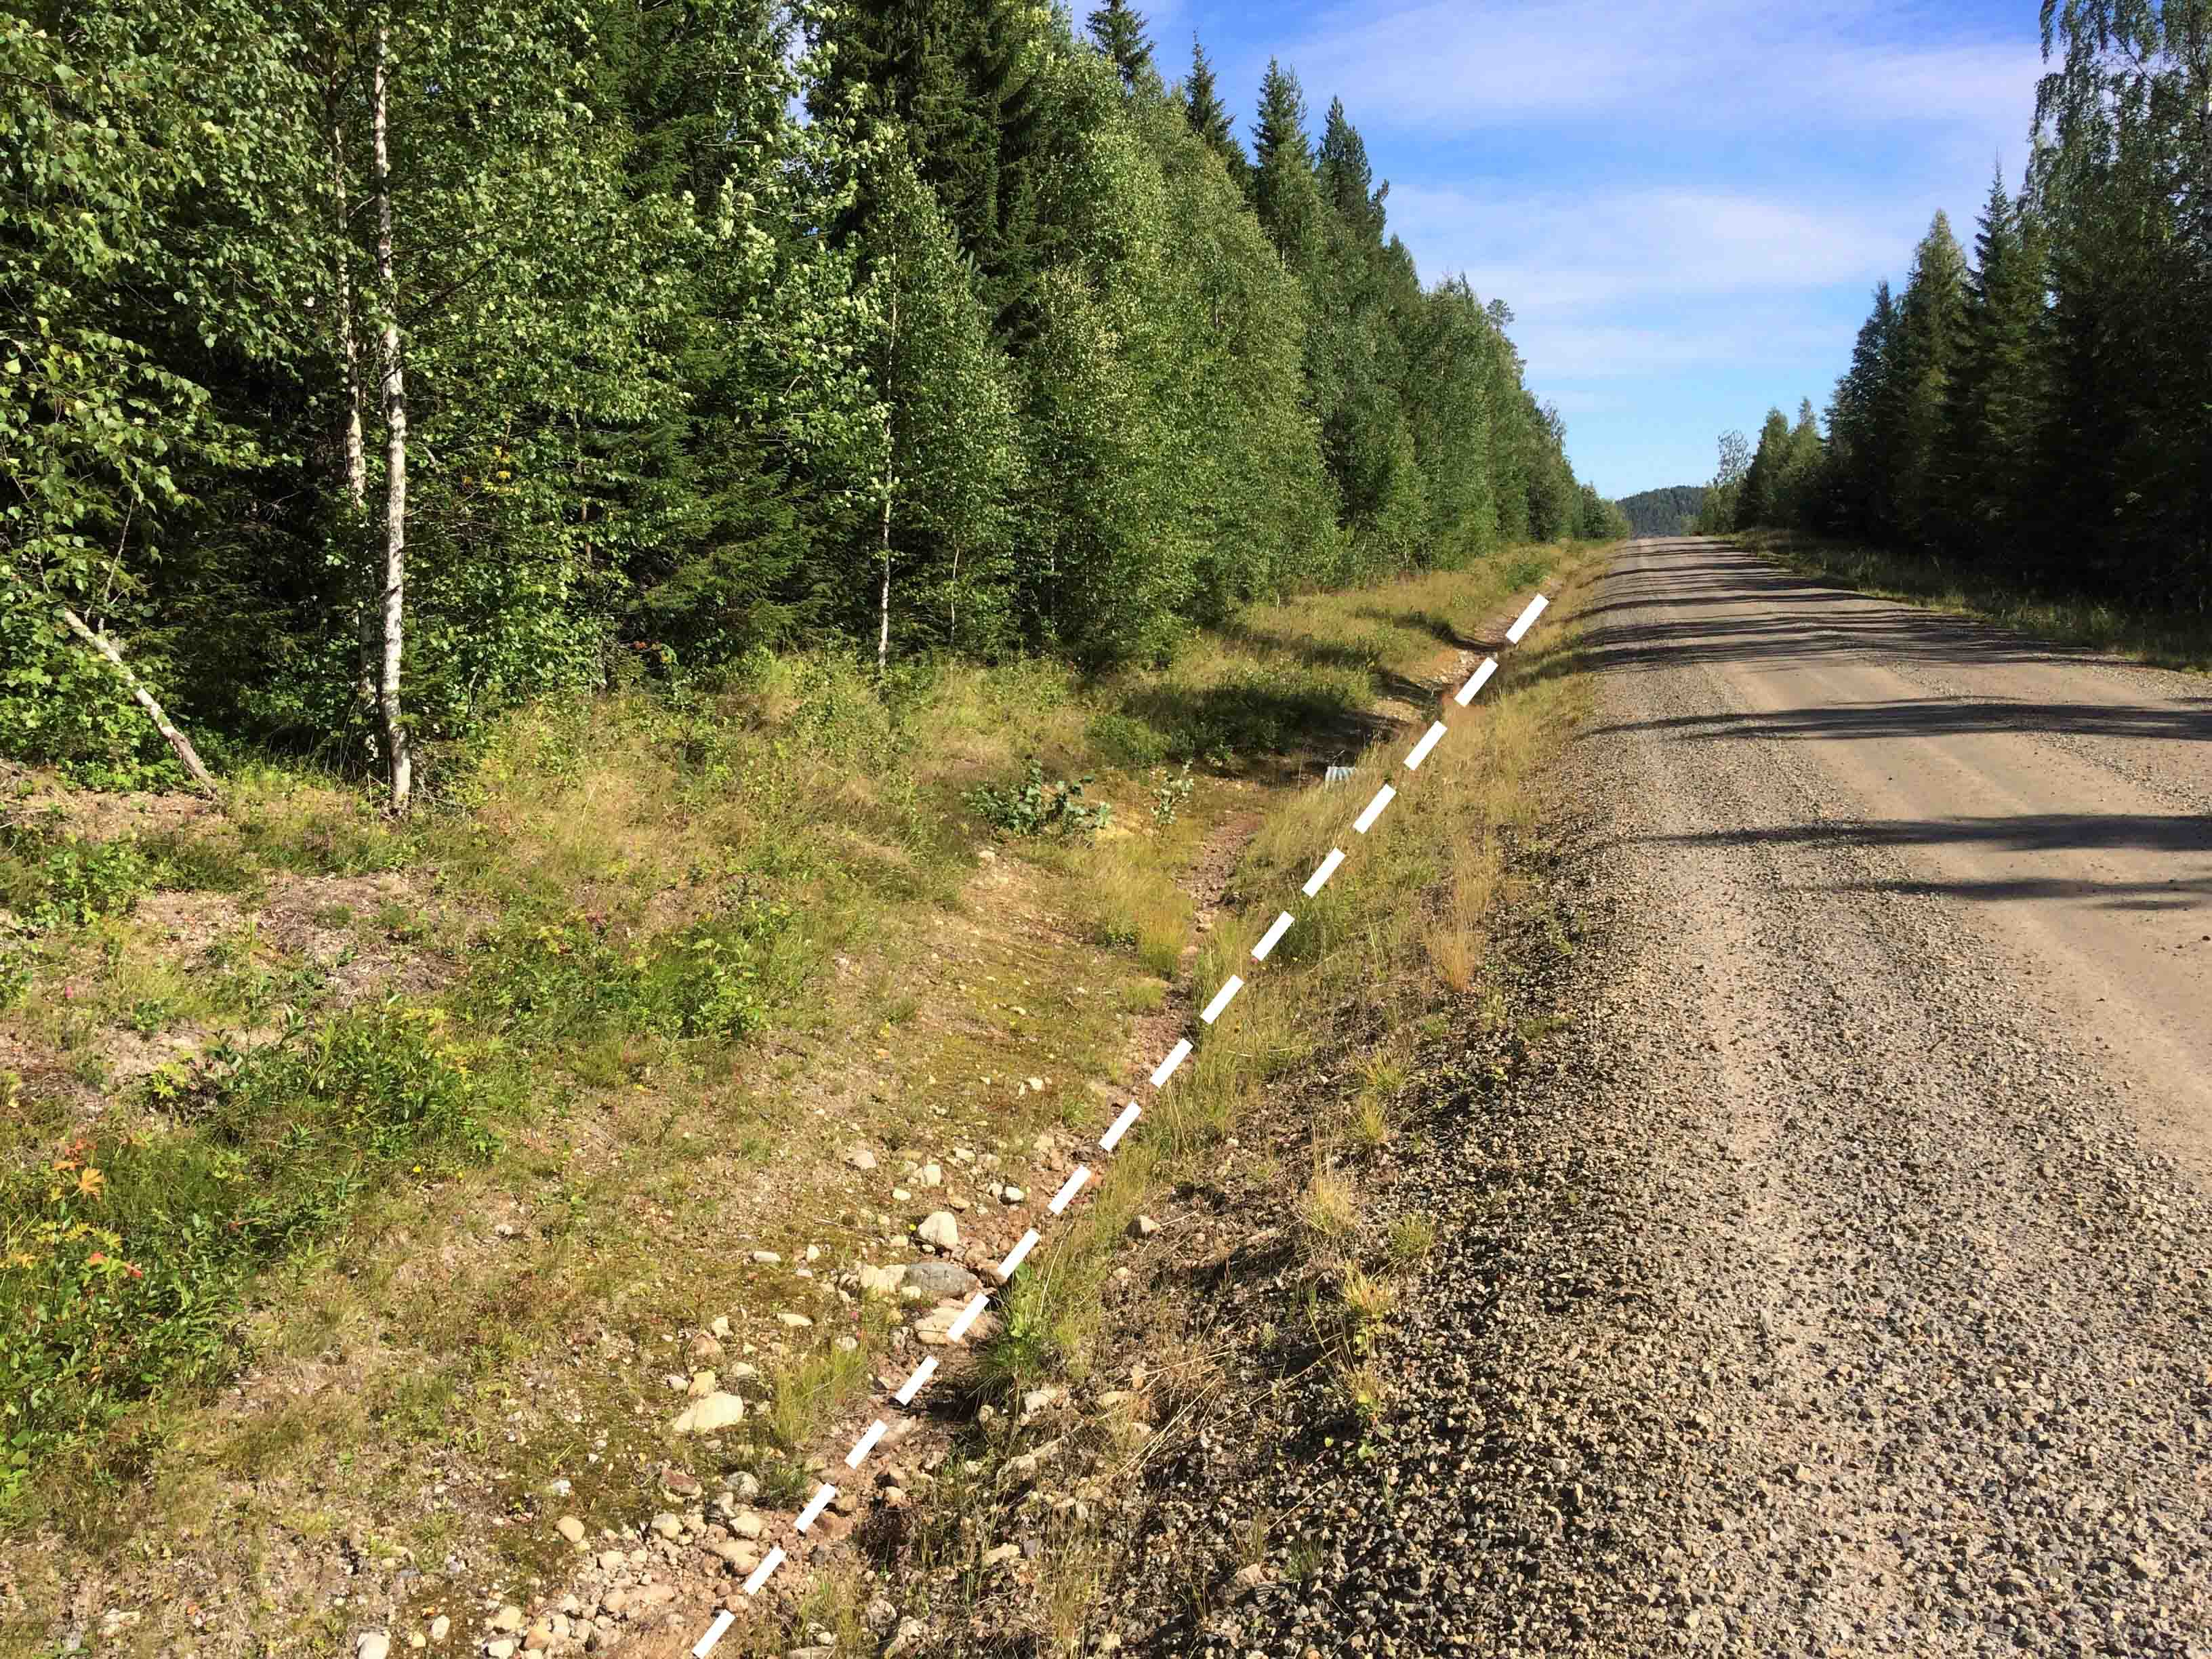
\includegraphics{./images/road_ditch_lo.jpg}}}\hspace{7pt}
    \subfigure[]{
        \resizebox*{6.85cm}{!}{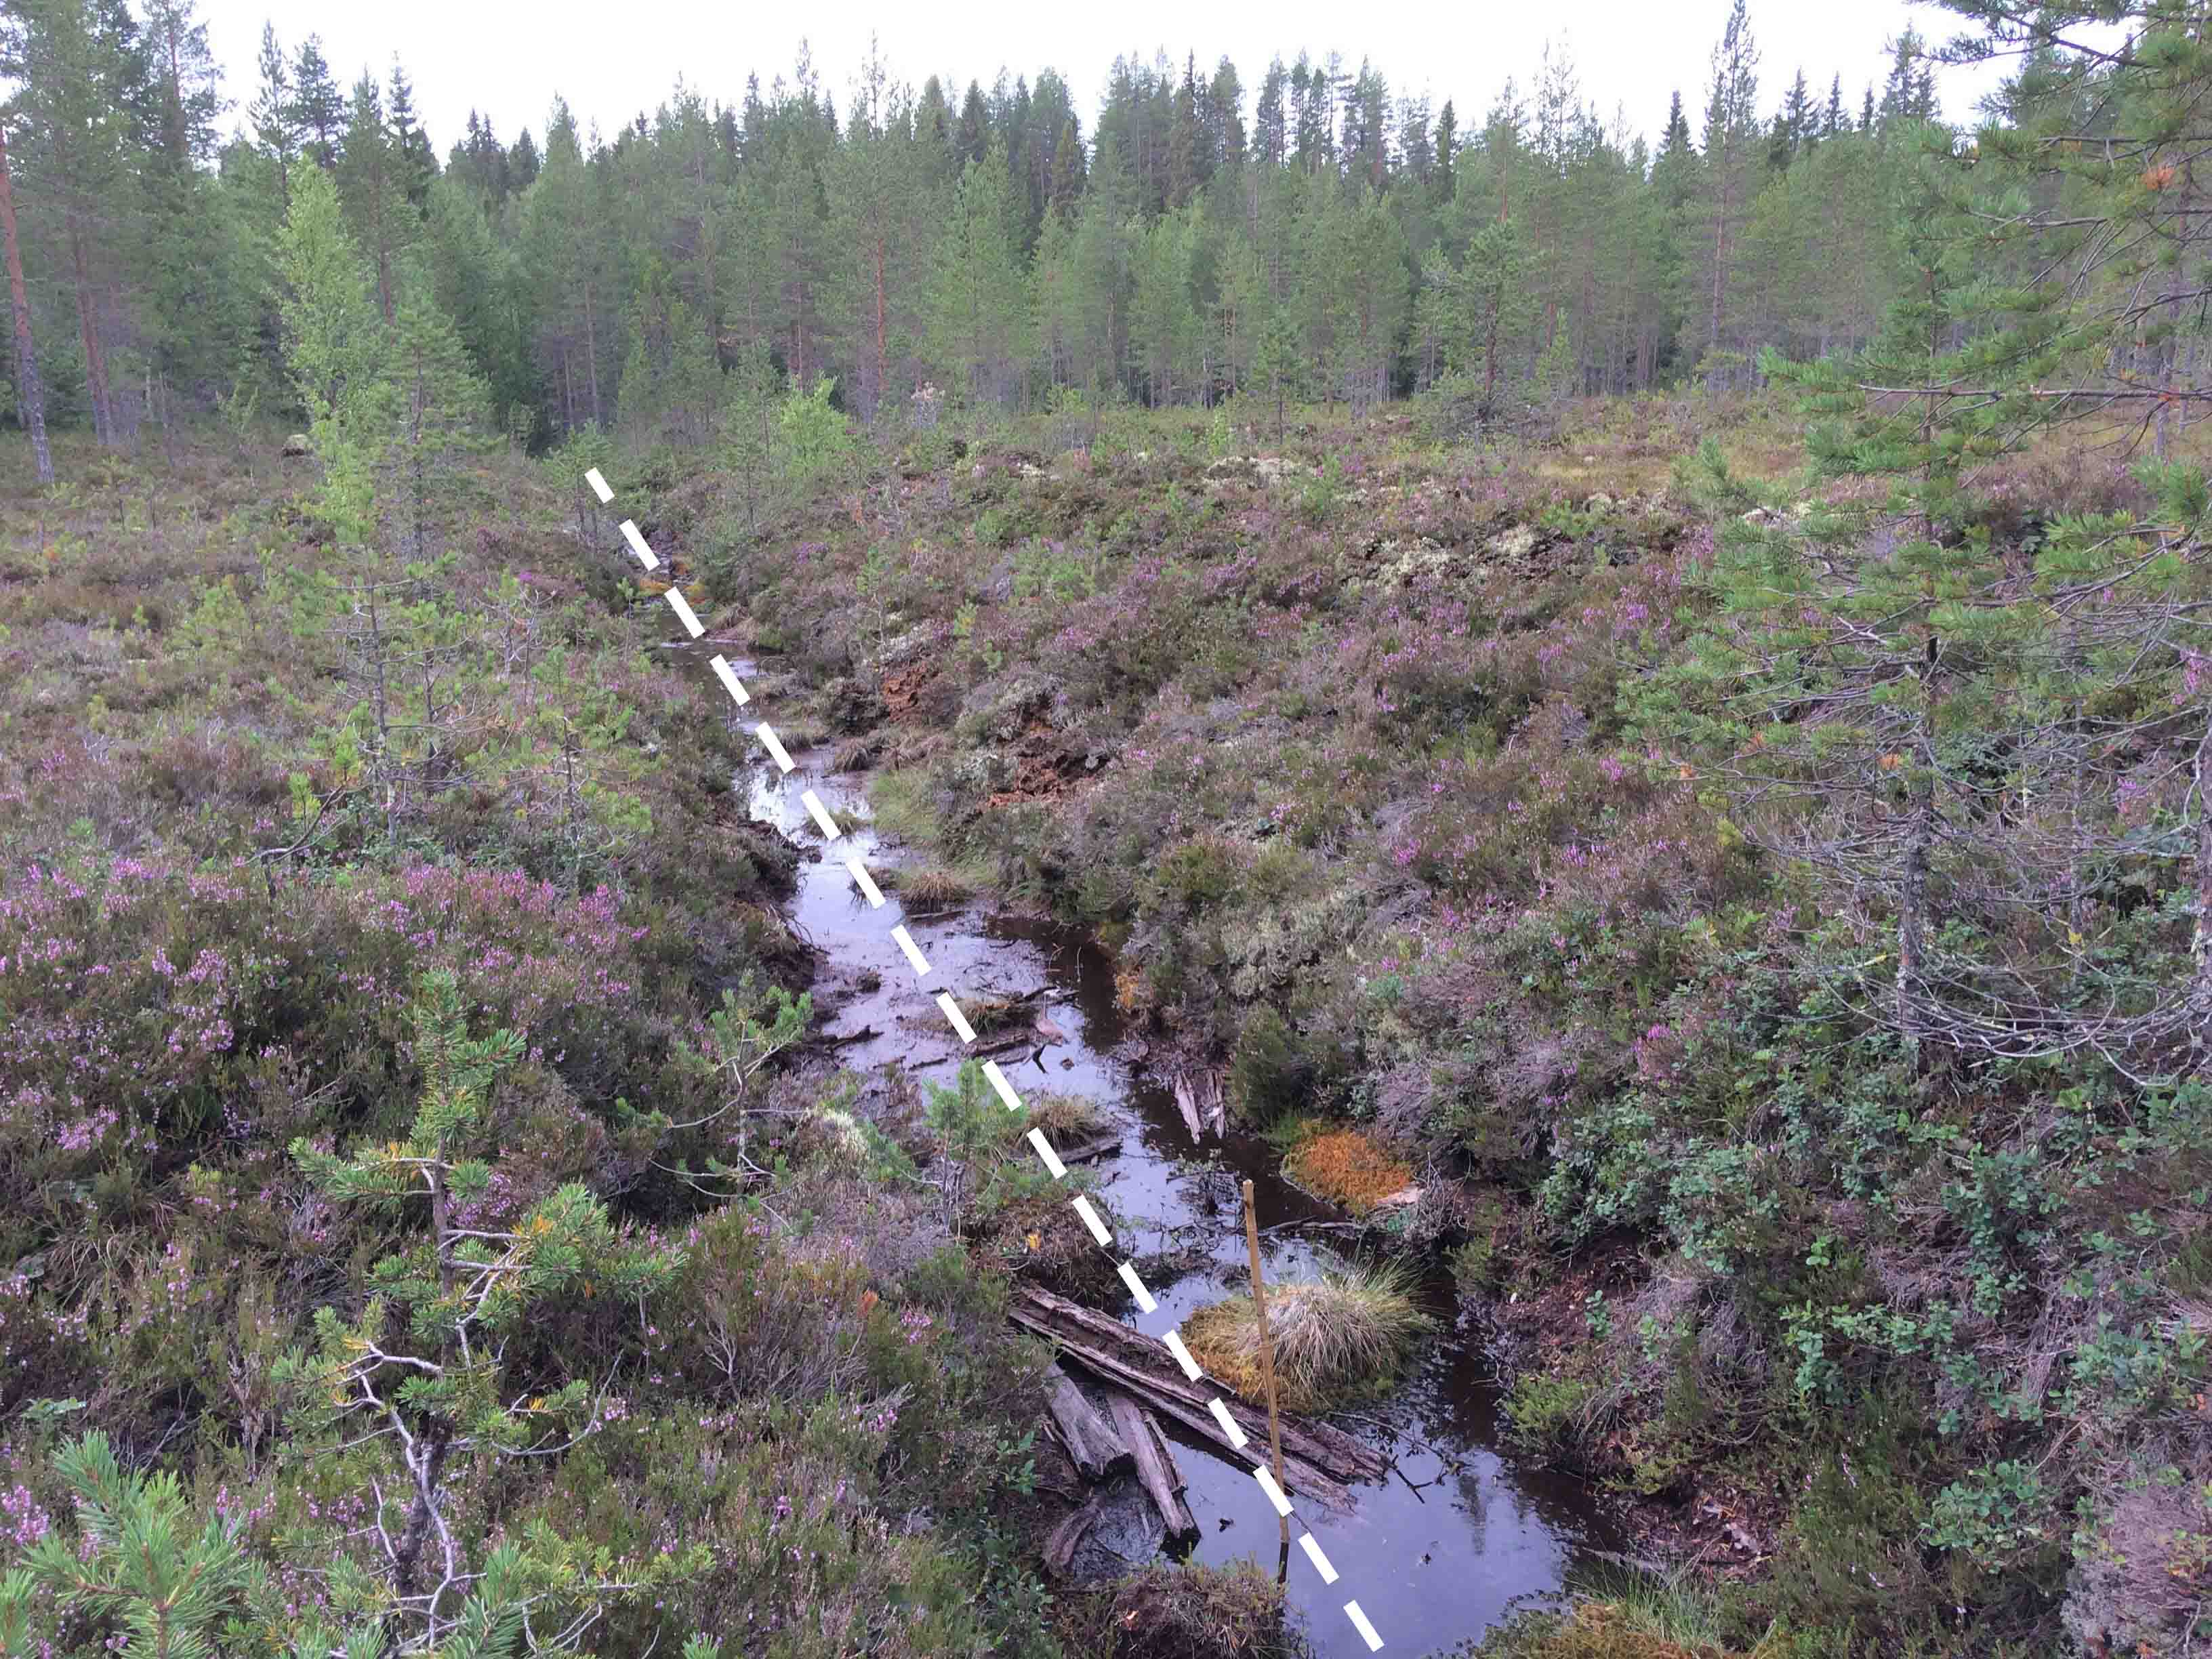
\includegraphics{./images/mire_ditch_lo.jpg}}}
    \subfigure[]{
        \resizebox*{6.85cm}{!}{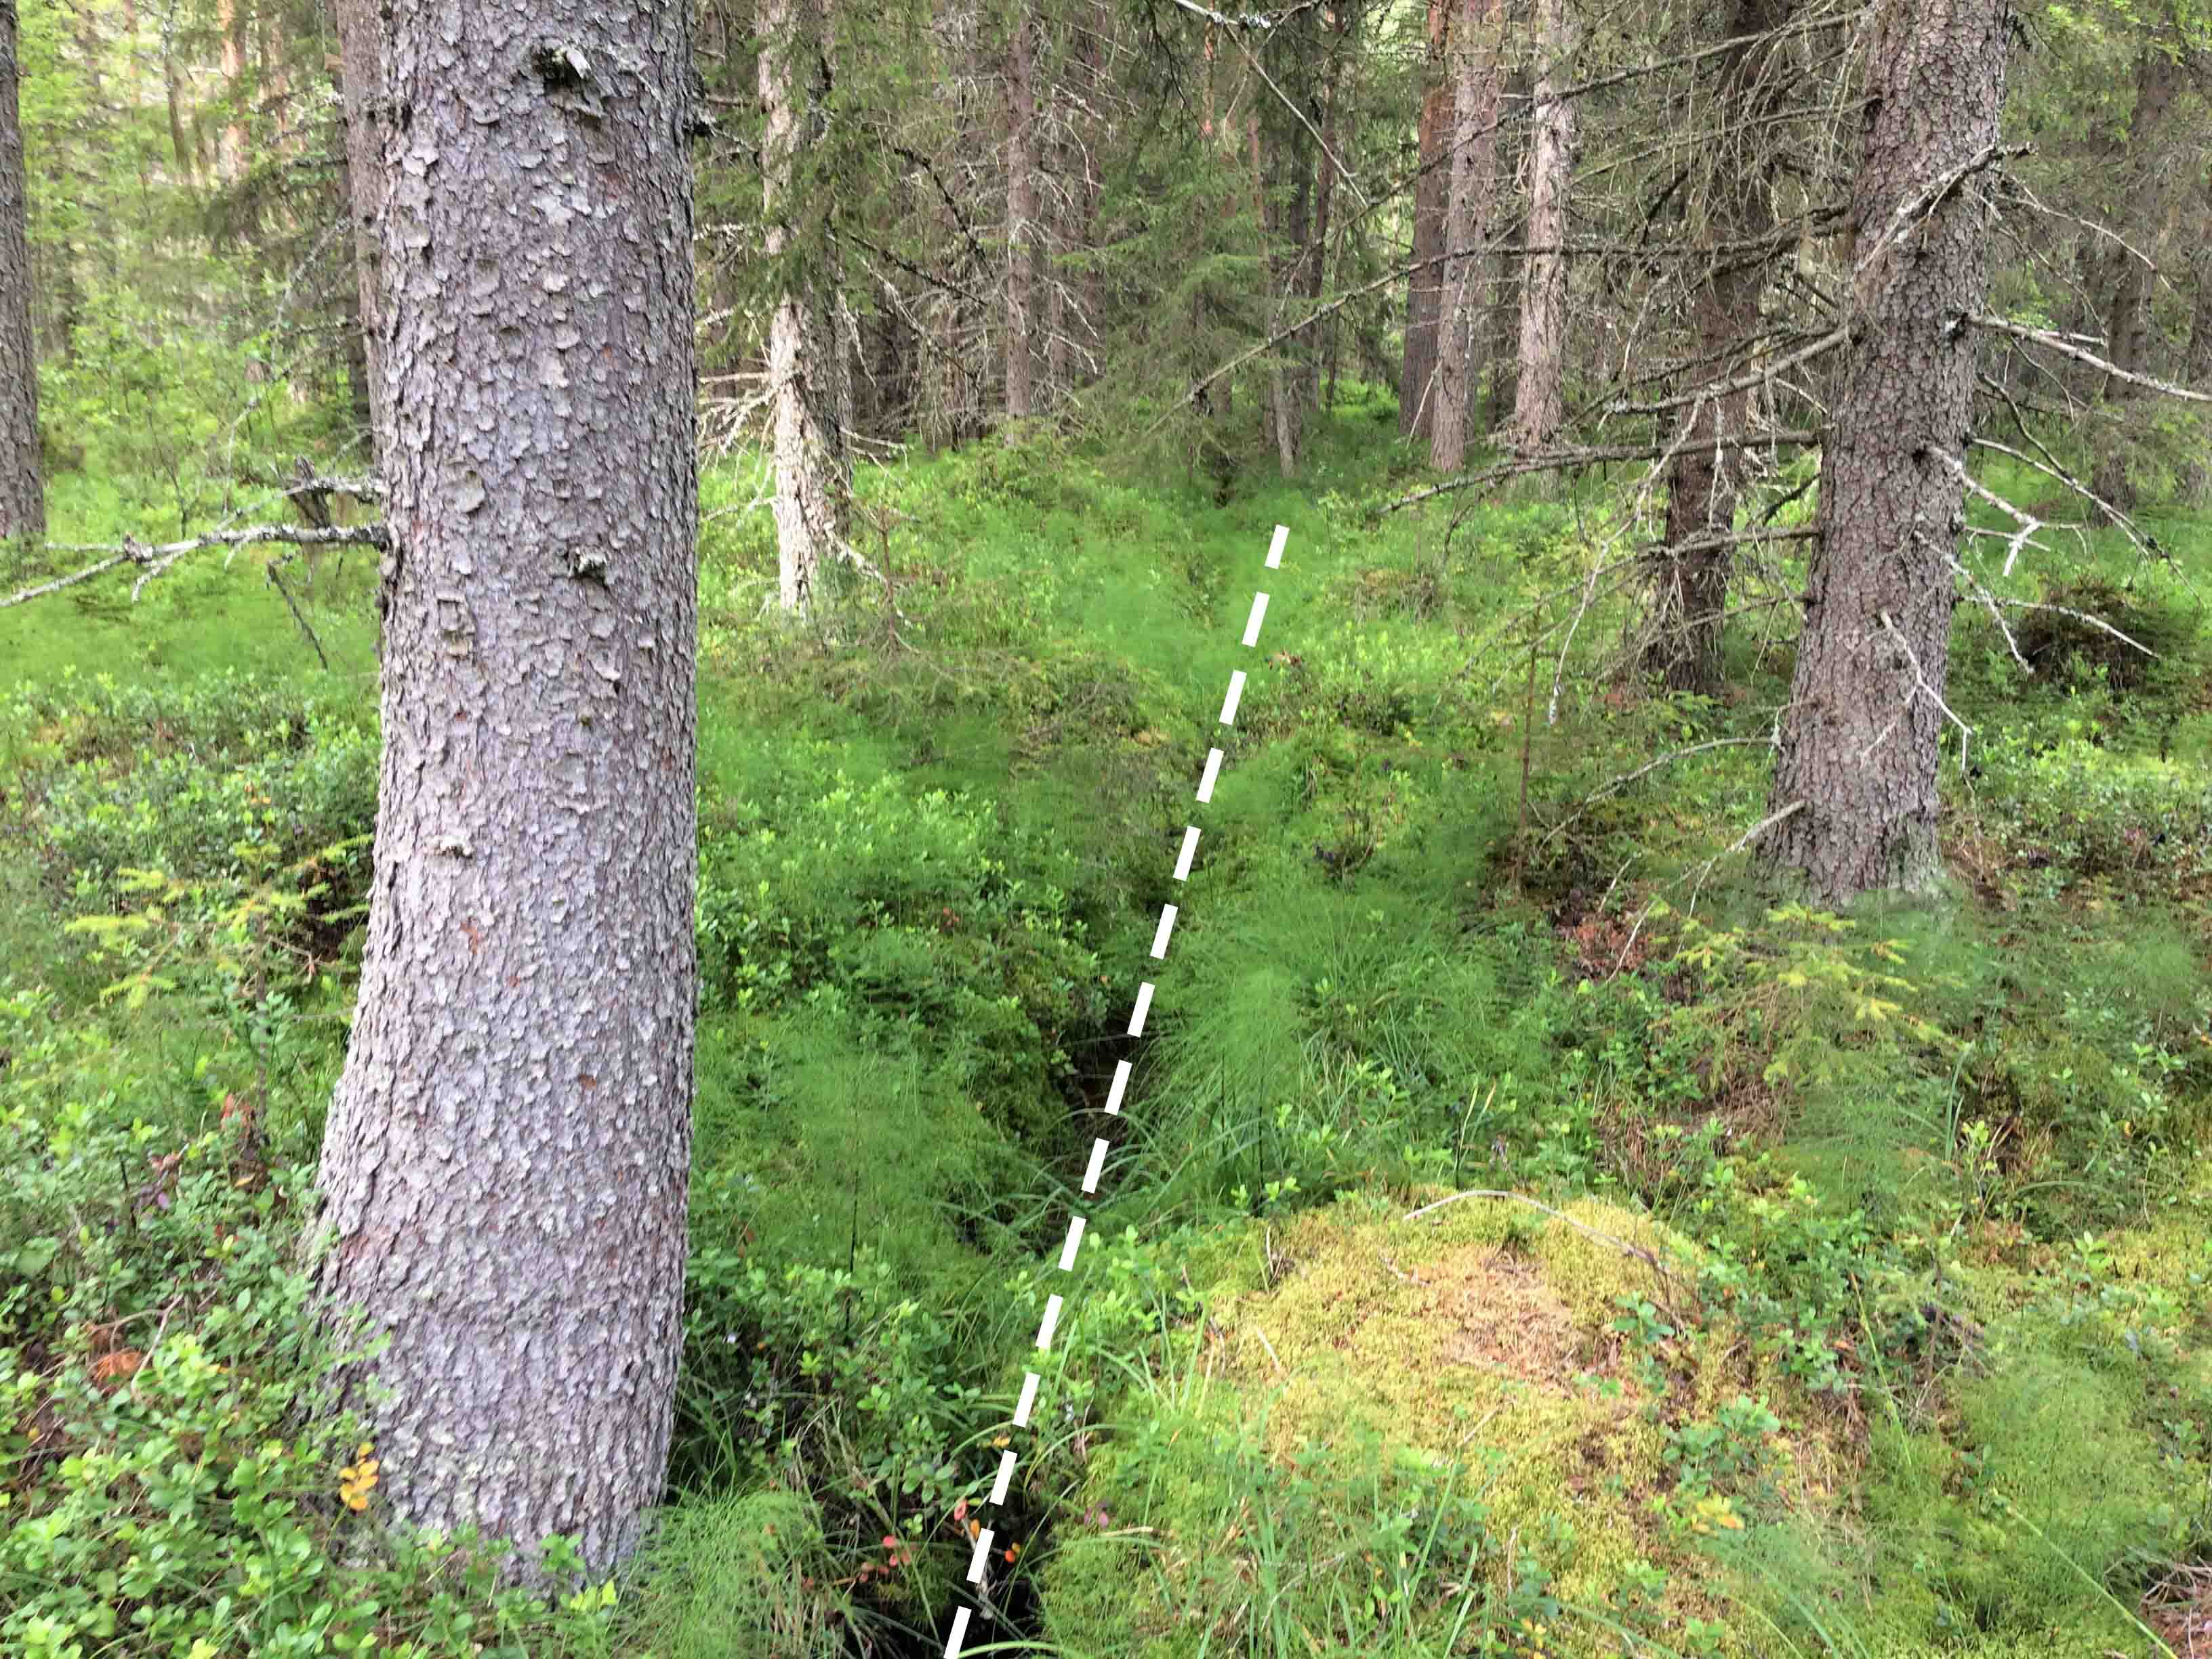
\includegraphics{./images/forest_ditch_lo.jpg}}}\hspace{7pt}
    \subfigure[]{
        \resizebox*{6.85cm}{!}{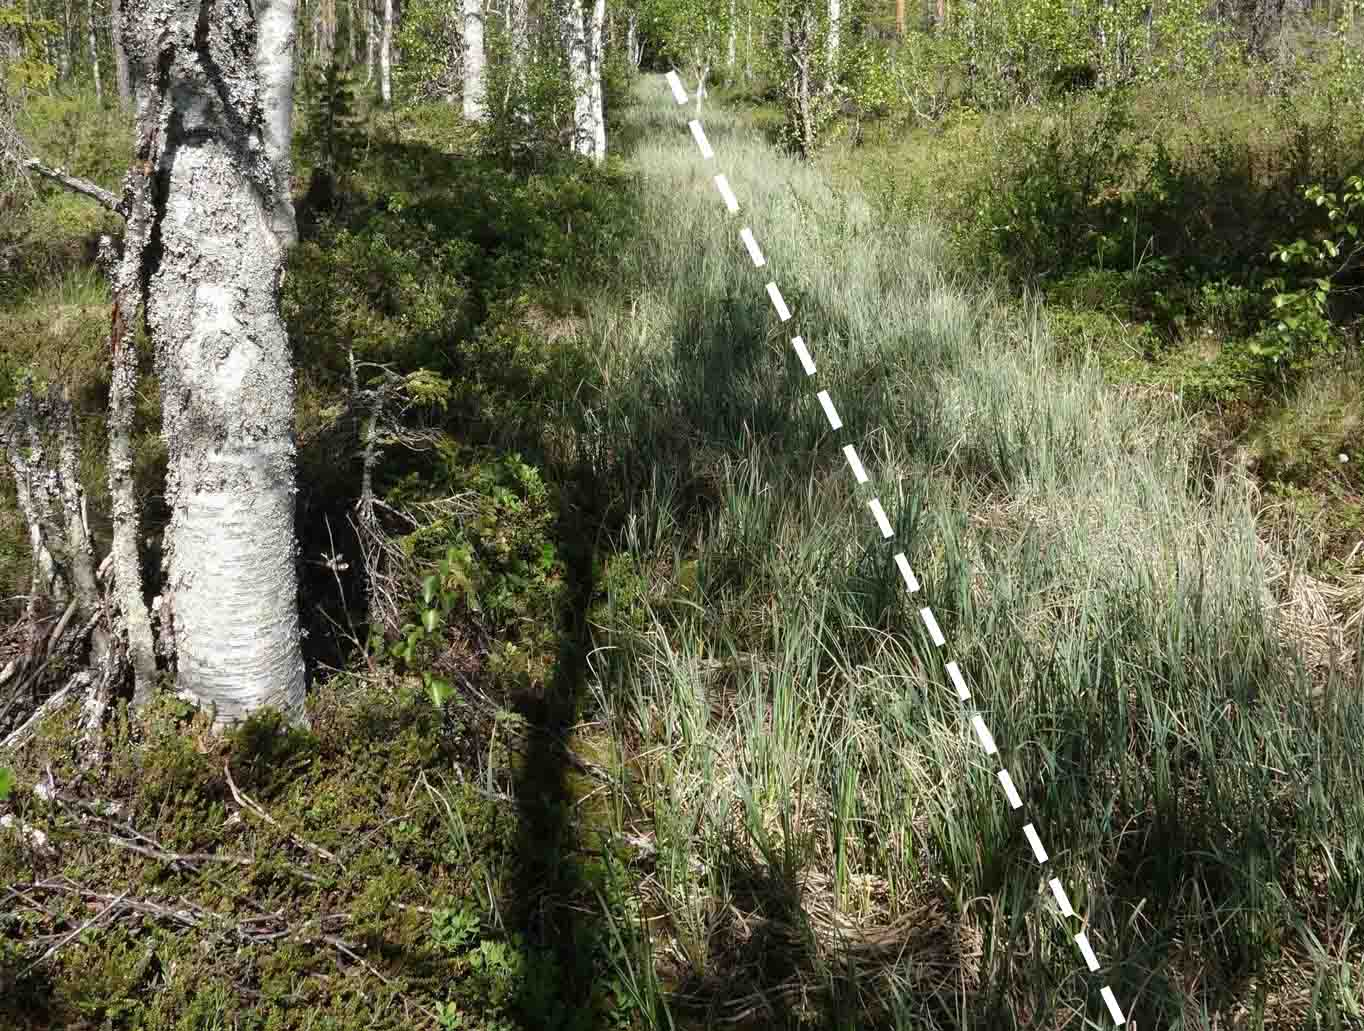
\includegraphics{./images/overgrown_ditch_lo.jpg}}}
    \caption{All photos show ditches in the study catchment. They illustrate the difficulty of capturing the ditches based on their form (i.e. an elongated, narrow, hollow in the ground). \textbf{a: }A roadside ditch. These are generally easily detected as they are usually found in open areas along the roads, and have often been maintained. \textbf{b: }A ditch in a mire; this is still easily detected, as there is no canopy and there is a clear elevation difference between the ditch and surrounding area. \textbf{c: }A narrow, more or less  overgrown ditch in a dense forest stand. \textbf{d: }A ditch in a mire that has more or less grown back in with \textit{Sphagnum sp.} and \textit{Carex}, likely also in combination with subsiding surrounding soils. Such ditches can be found in the field as the vegetation differs, but as there is no longer an elevation difference between the ditch and the surrounding soils it will not be detected in the DEM. Photos a-c: E. Maher Hasselquist  Photo d: G. Norstedt}
    \label{fig:ditchpictures}
\end{figure}

Hypothetically, it should be quite easy to detect ditches using LiDAR data. In practice, however, there are many variables affecting the results\DIFdelbegin \DIFdel{. One is }\DIFdelend \DIFaddbegin \DIFadd{, such as }\DIFaddend the point density and the interpolation method used to create the DEM. \citet{rapinel} found that the results were usually more sensitive to the point density (ranging 1-4 points $m^{2}$ in their study) than the interpolation method. They retrieved 54.8 and 63.8 \% of the ditches on the Acuey and Boucey marches in France, compared to \DIFdelbegin \DIFdel{77.4 }\DIFdelend \DIFaddbegin \DIFadd{70.28 }\DIFaddend \% in our study. However, in our study we had a point density of 20 points $m^{2}$, so the quality of the DEM in our study ought to be robust, which may have contributed to our higher retrieval rate. \hyperref[fig:resultstreesbushes]{Figure} \ref{fig:resultstreesbushes} \hyperref[fig:resultstreesbushes]{(a, b)} illustrates the difference in the quality of the LiDAR data where the laser pulses have caught in trees or shrubs. When too few LiDAR points reach the ground, the DEM generation is forced to interpolate over a larger area, leading to inaccuracies in the ground DEM.

\begin{figure} [!htb]
    \centering
    \subfigure[]{
        \resizebox*{6.8cm}{!}{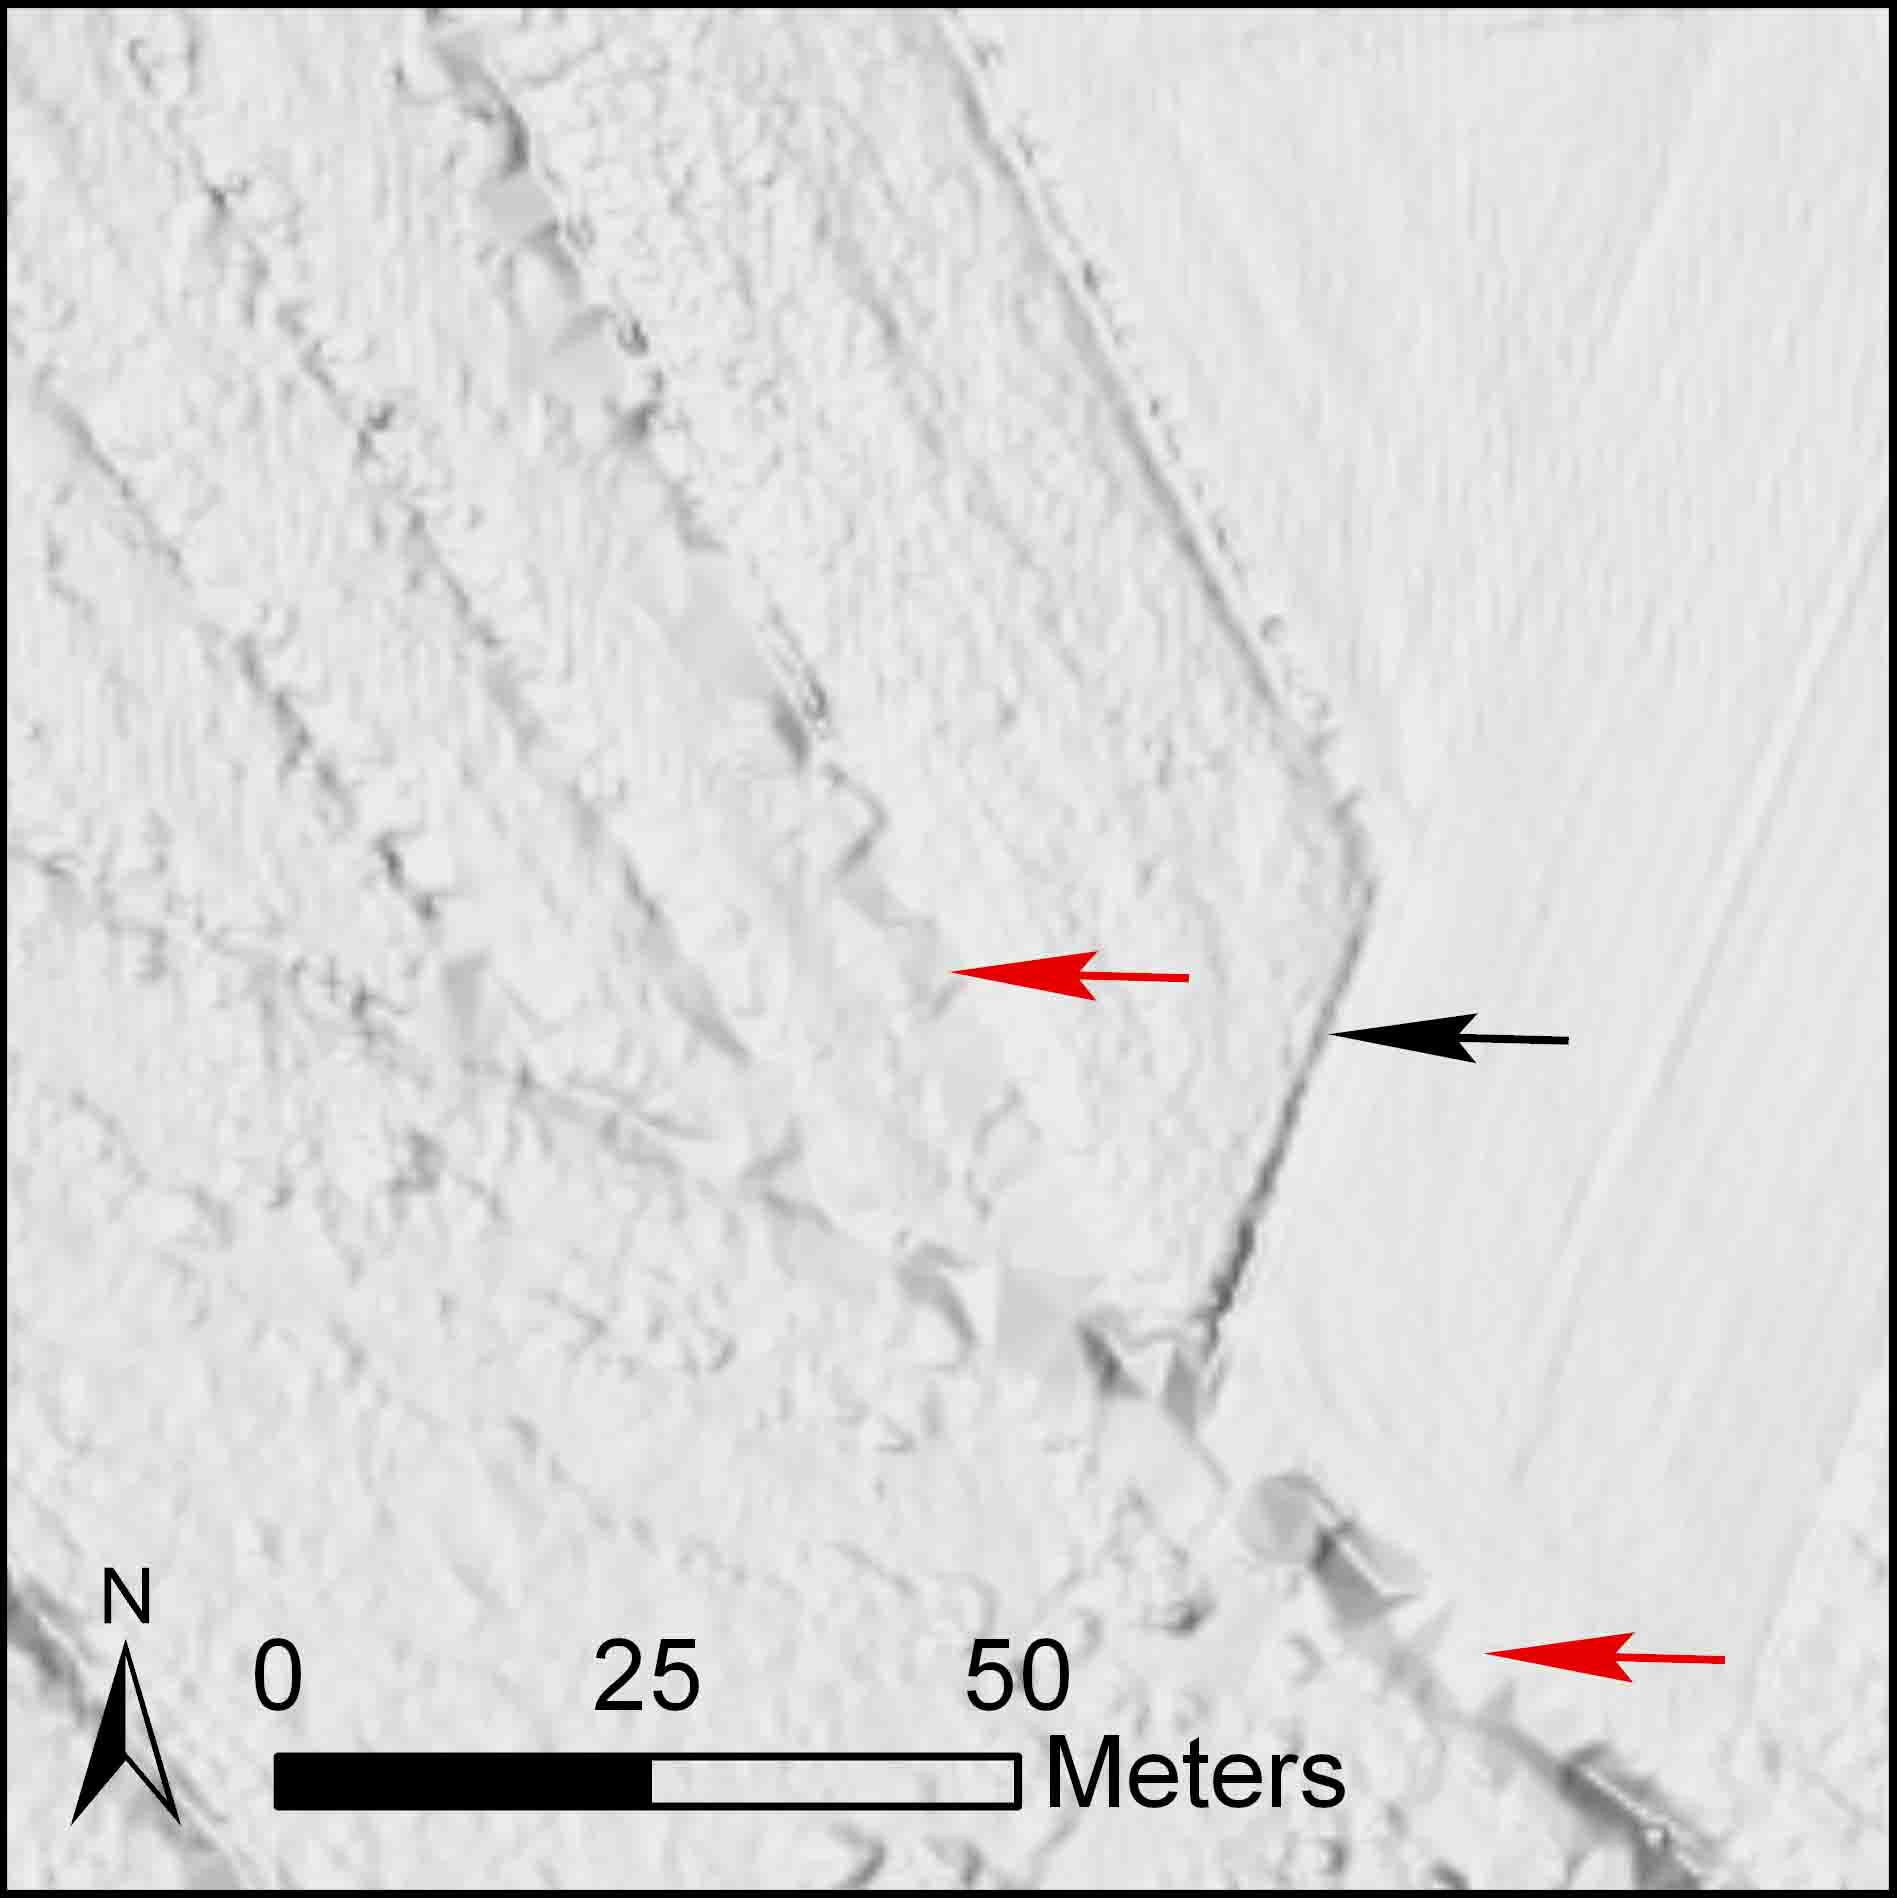
\includegraphics{./images/results_trees_bushes_1_lo.jpg}}}\hspace{7pt}
    \subfigure[]{
        \resizebox*{6.8cm}{!}{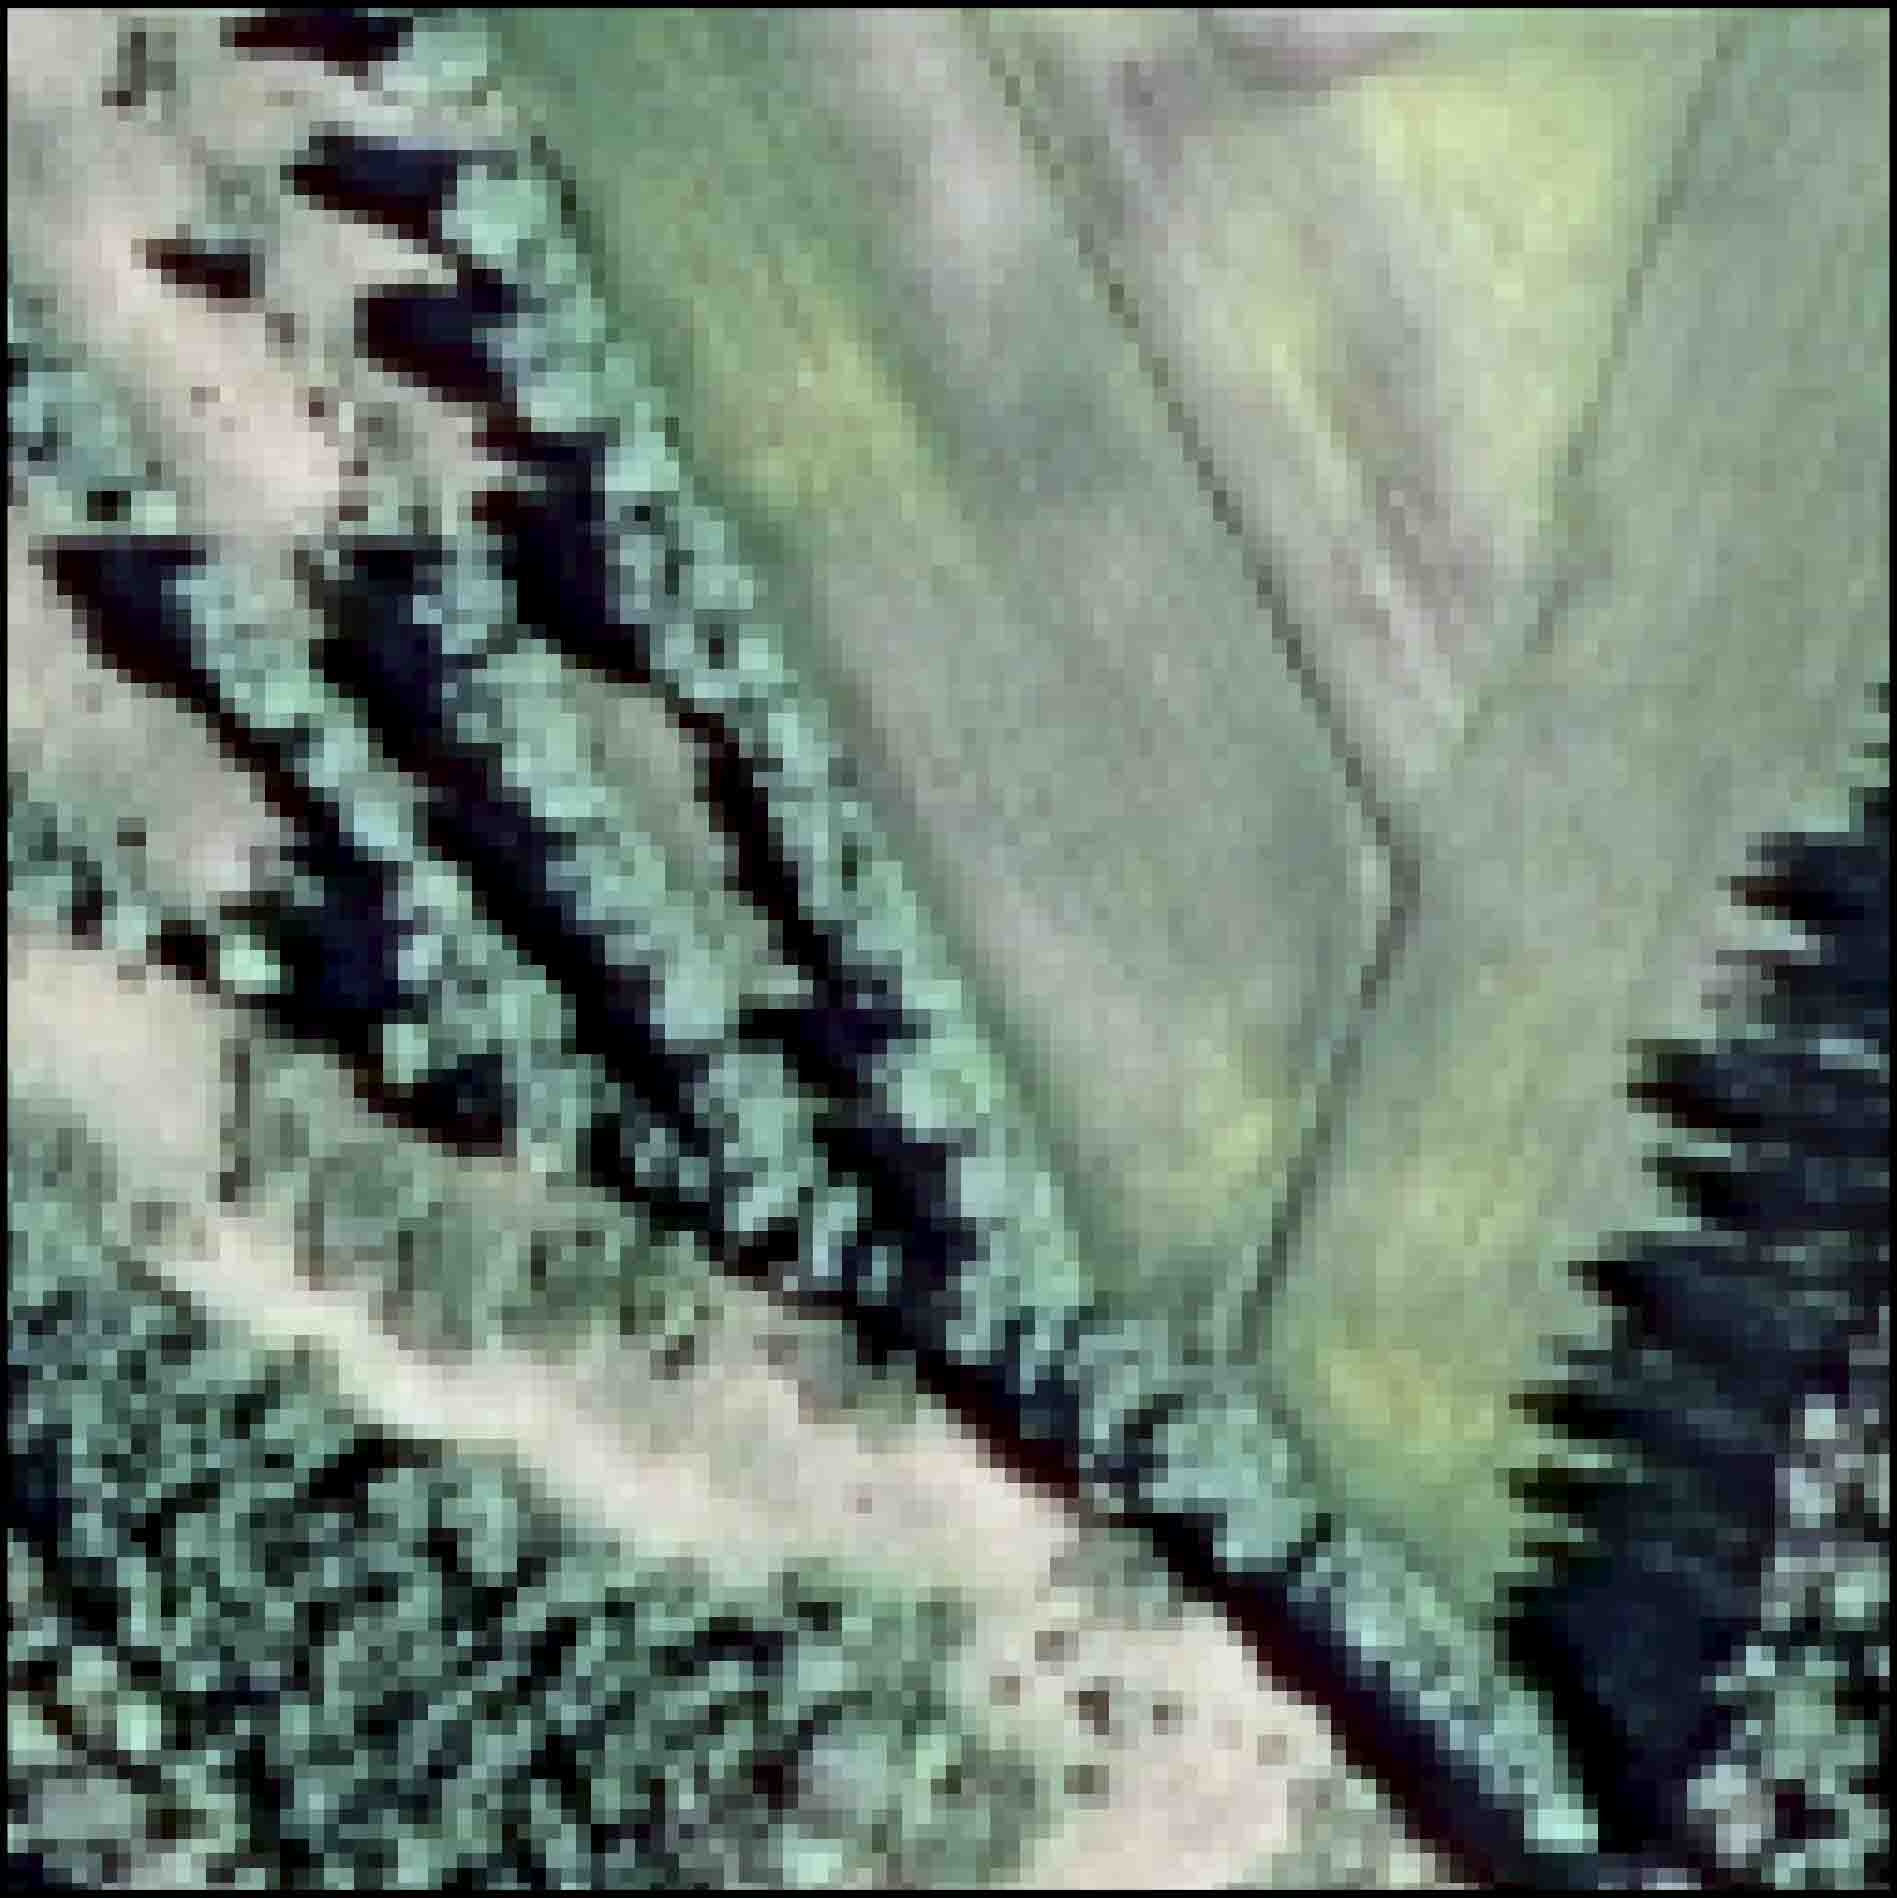
\includegraphics{./images/results_trees_bushes_2_lo.jpg}}}
    \subfigure[]{
        \resizebox*{6.8cm}{!}{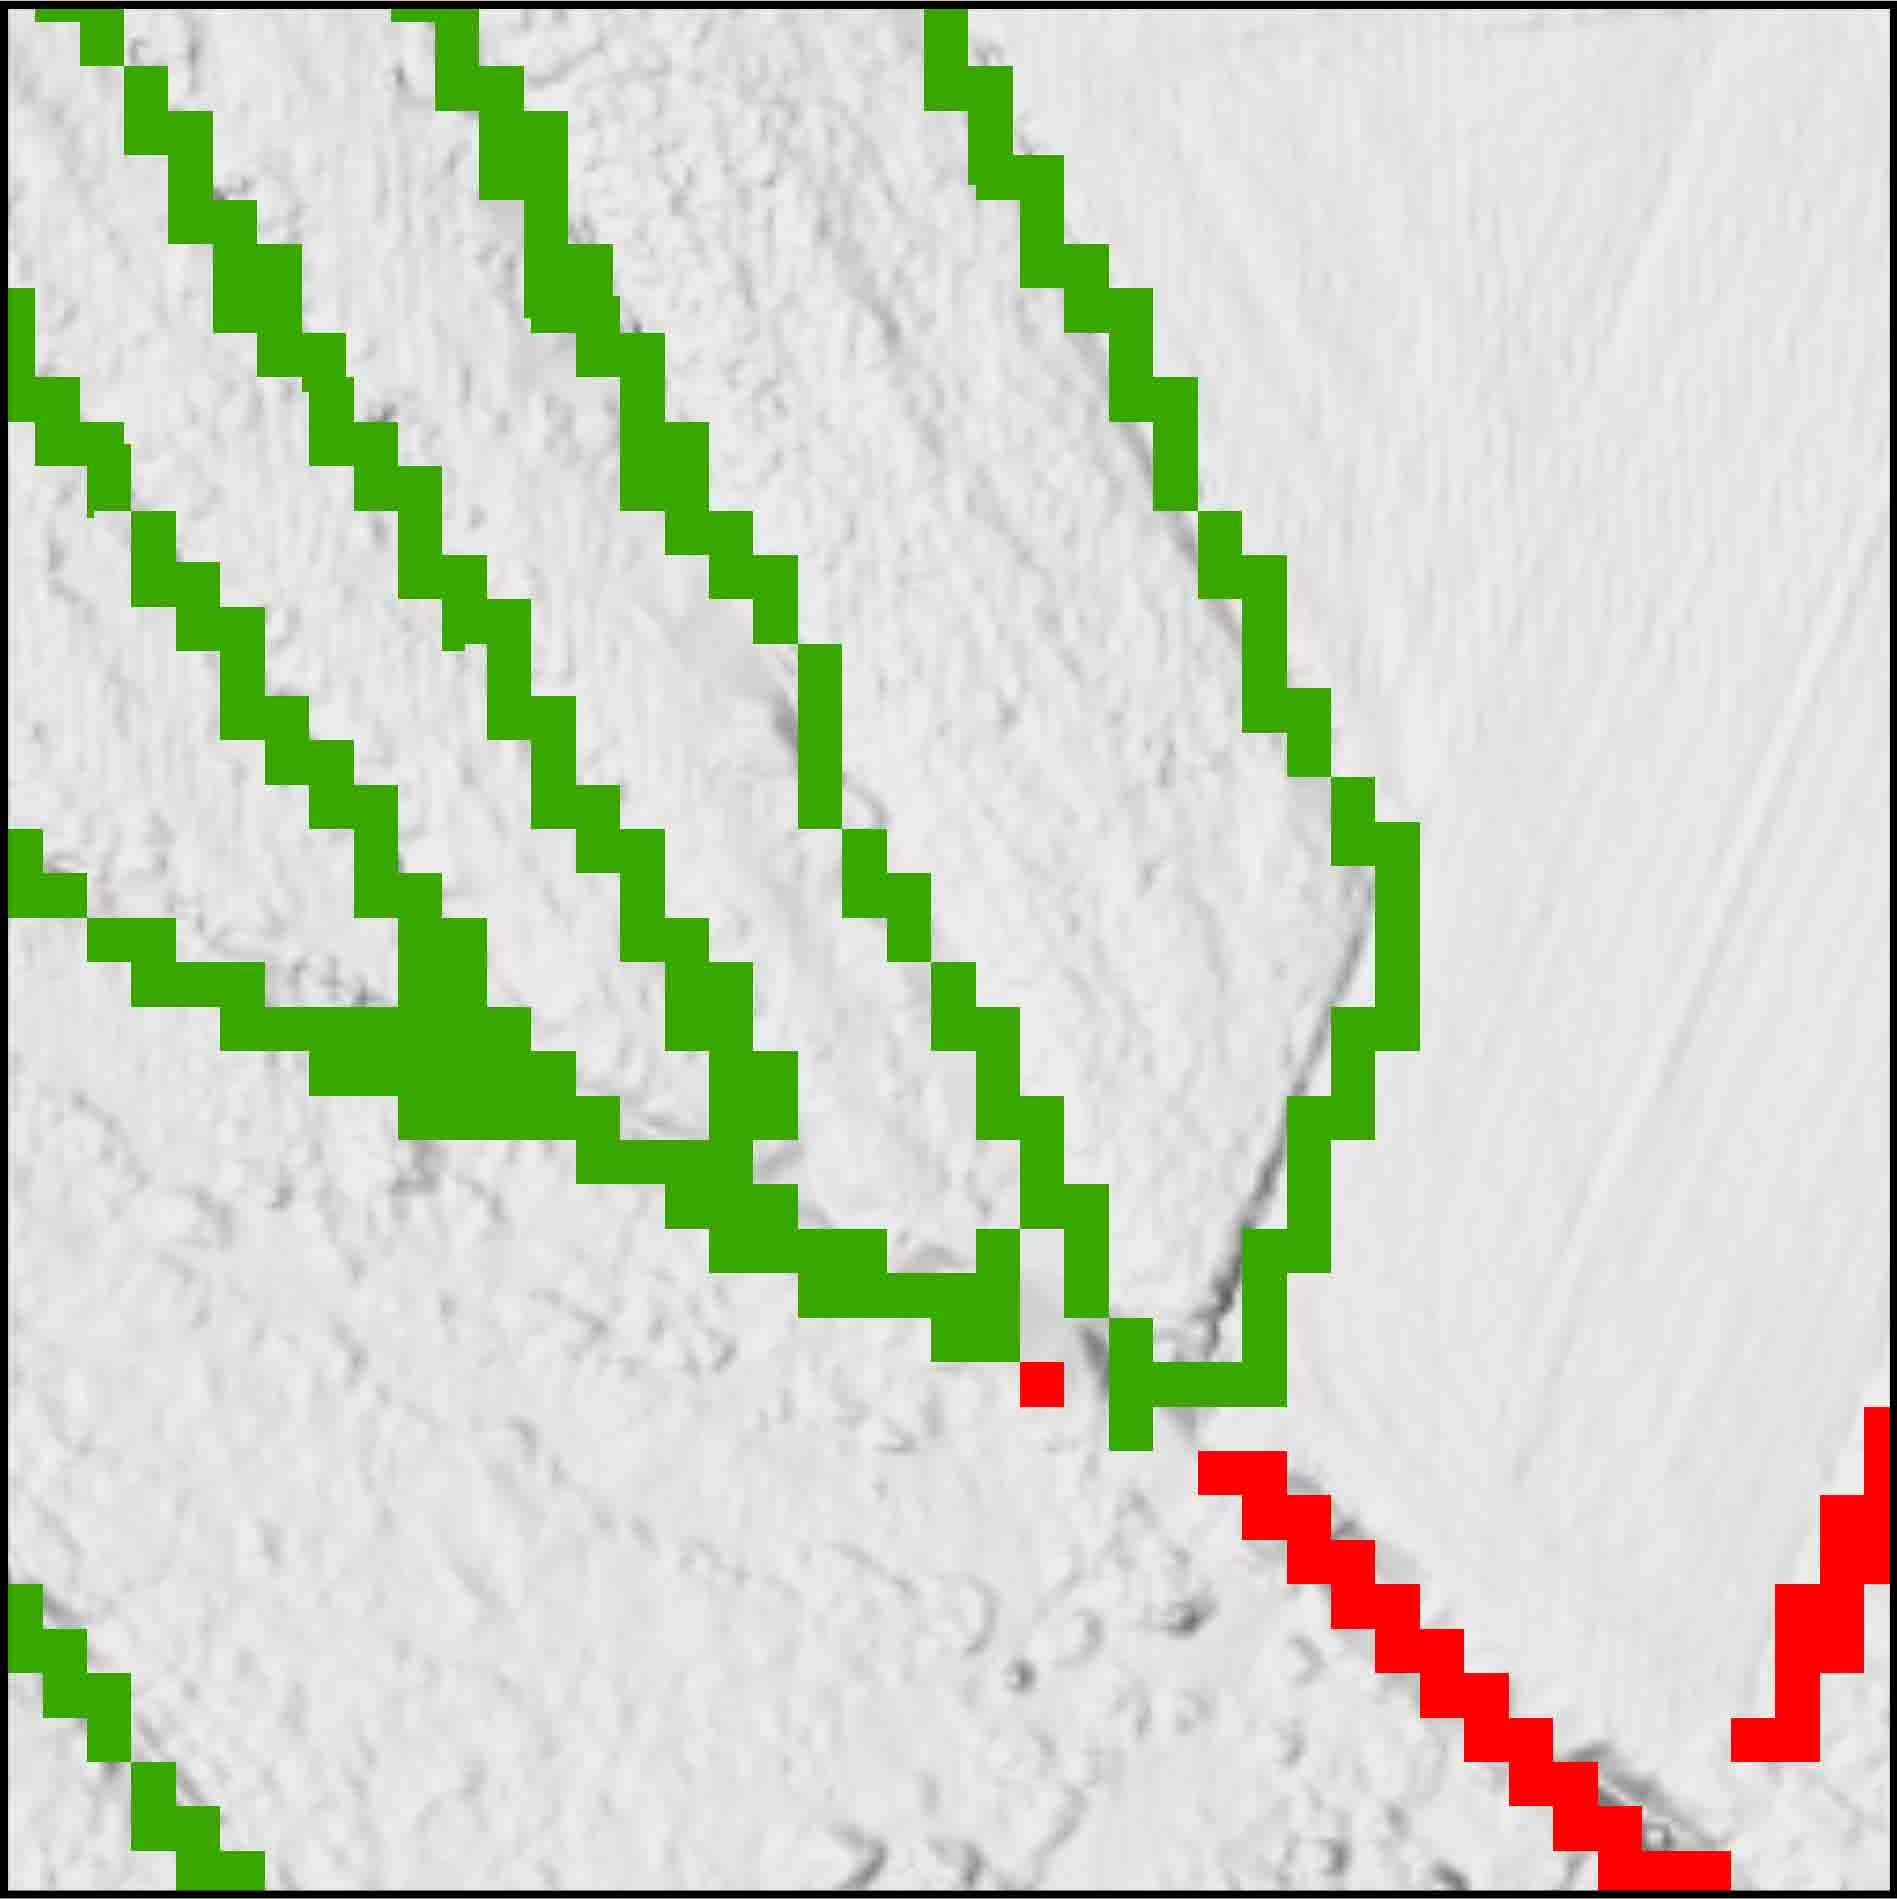
\includegraphics{./images/results_trees_bushes_3_lo.jpg}}}\hspace{7pt}
    \subfigure[]{
        \resizebox*{6.8cm}{!}{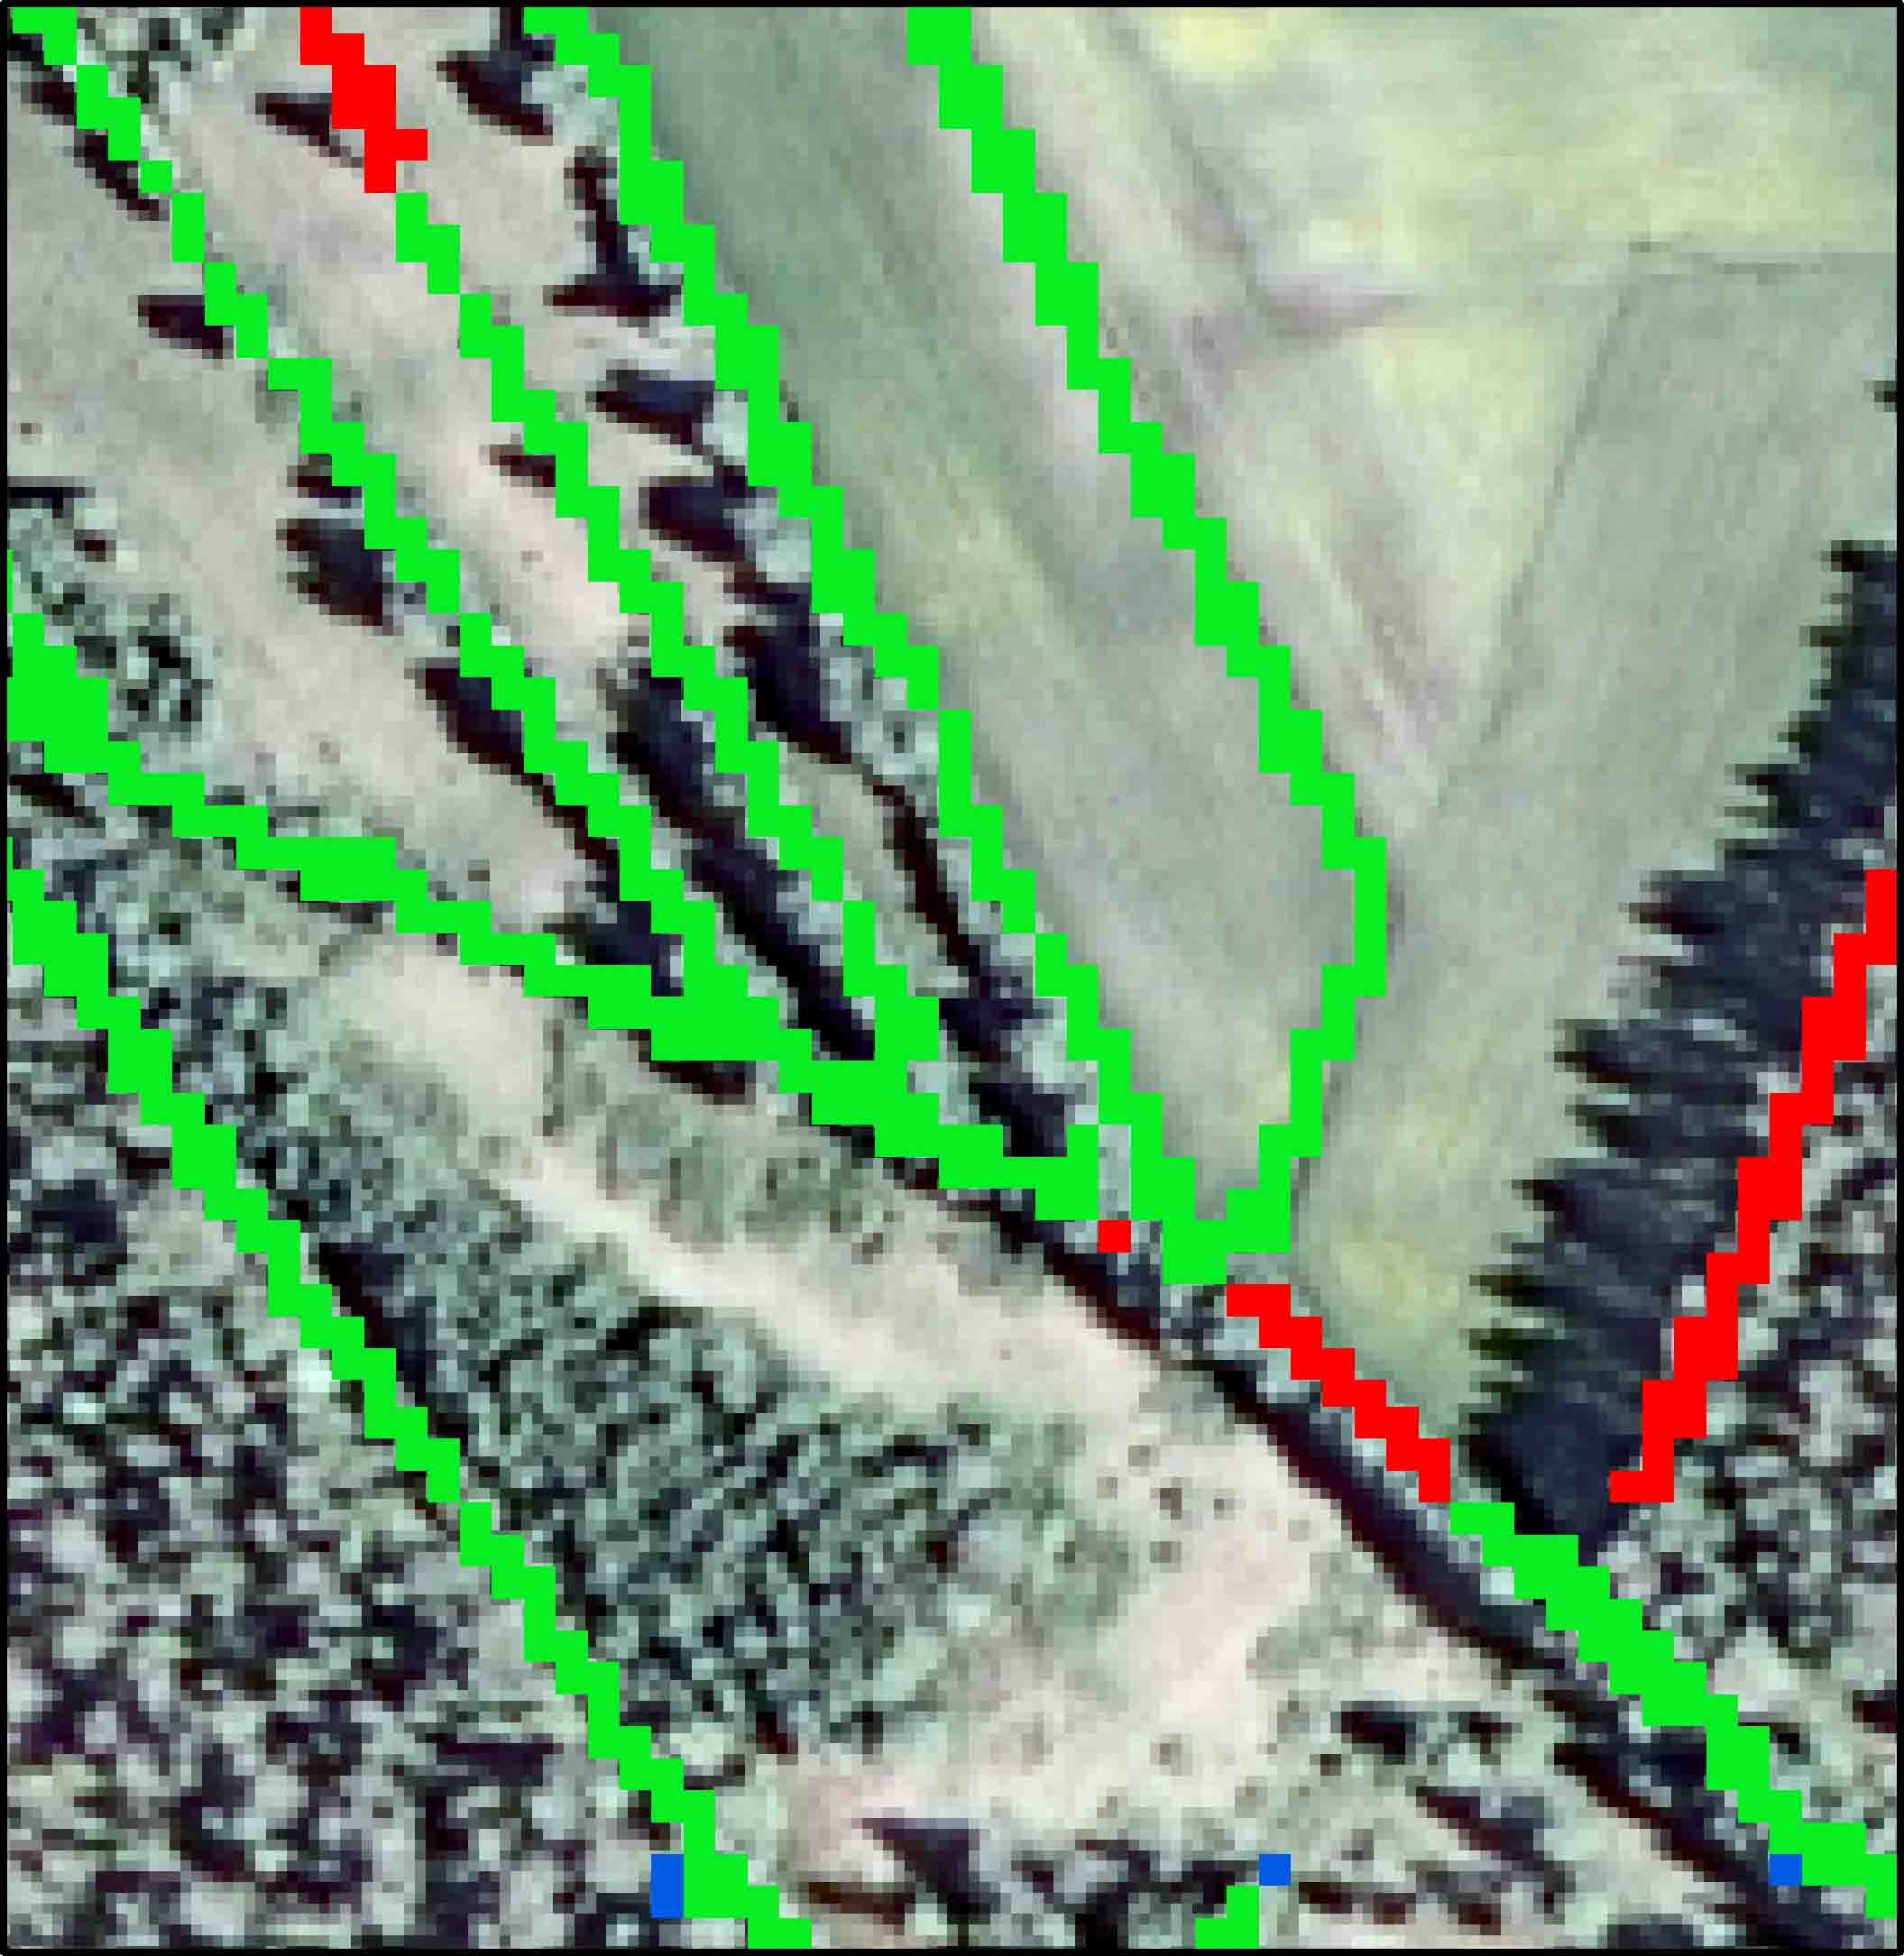
\includegraphics{./images/results_trees_bushes_4_lo.jpg}}}
    \caption{\textbf{a} and \textbf{b} illustrate that despite a point density of 20 points $m^2$, not all points reach the ground in places with dense vegetation. In \textbf{a} there is a clear difference between the smooth surface of the DEM in the open area (black arrow), and in the areas covered by trees and shrubs (red arrows), where the DEM is much coarser due to interpolation with a lower number of LiDAR points here. The orthophoto (\textbf{b}), clearly shows that trees and shrubs are growing in the ditches in this area. This makes it more difficult to detect ditches. However, despite these coarser grid points in the DEM, \textbf{c} and \textbf{d} shows that the \DIFdelbeginFL \DIFdelFL{model }\DIFdelendFL \DIFaddbeginFL \DIFaddFL{ditch detector }\DIFaddendFL still managed to capture a majority of the ditches (green), and only failed at certain points (red).}
    \label{fig:resultstreesbushes}
\end{figure}

\DIFaddbegin \DIFadd{With our method, natural streams were often classified as false positives (}\hyperref[fig:resultsillustrations]{Figure} \DIFadd{\ref{fig:resultsillustrations} }\hyperref[fig:resultsillustrations]{b}\DIFadd{) as our aim was focused on locating ditches. However, this indicates that our method could also be used to map small, previously unmapped natural stream channels. The national survey showed that 55\% of the natural stream channels and 75\% of the straightened water courses were missing on the maps. This is in line with other national \mbox{%DIFAUXCMD
\citep{kuglerova} }\hspace{0pt}%DIFAUXCMD
and international \mbox{%DIFAUXCMD
\citep{benstead} }\hspace{0pt}%DIFAUXCMD
studies highlighting this phenomenon called "Aqua Incognita - the unknown headwaters" \mbox{%DIFAUXCMD
\citep{bishop,kuglerova}}\hspace{0pt}%DIFAUXCMD
.
}

\DIFaddend The results from our method (\hyperref[predictionperformance]{Table} \ref{predictionperformance}) show that we managed to attain a Cohen's $\kappa$ rating in the substantial range, according to performance thresholds proposed by \citet{kappaanalysis}. \DIFdelbegin \DIFdel{This means that our model performed substantially better than one based purely on chance. }\DIFdelend The total recall value of \DIFdelbegin \DIFdel{77.4 }\DIFdelend \DIFaddbegin \DIFadd{70.28 }\DIFaddend \% shows that we managed to find a majority of the ditch pixels that exist. The results of our method also showed a significant improvement for ditch detection over classifying with the digital terrain indices separately \DIFaddbegin \DIFadd{(}\hyperref[recreatedpredictionperformance]{Table} \DIFadd{\ref{recreatedpredictionperformance})}\DIFaddend . Had we been able to use labels that were correctly labelled on a pixel basis, i.e. each ditch had its actual width recorded, the \DIFdelbegin \DIFdel{model }\DIFdelend \DIFaddbegin \DIFadd{models }\DIFaddend could have learned with a better accuracy in the training phase, and the classification results would also most likely have benefitted from this.

Sometimes pixels in ditches were initially identified correctly as ditch pixels, but because not enough pixels in the surrounding area were detected, the post-processing algorithms identified them as noise and removed them. Incorrectly classified ditch pixels that caused the precision to decrease were generally the pixels that lay in streams (\hyperref[fig:resultsillustrations]{Figure} \ref{fig:resultsillustrations} \hyperref[fig:resultsillustrations]{a, b}). However, small \DIFdelbegin \DIFdel{cavities }\DIFdelend \DIFaddbegin \DIFadd{sinks }\DIFaddend or hilly areas incorrectly classified as ditches by the \DIFdelbegin \DIFdel{model }\DIFdelend \DIFaddbegin \DIFadd{Random Forests models }\DIFaddend were generally removed in the post-processing. We managed to bridge gaps and exclude streams to some extent in our predictions. This was in part due to the post-processing of the prediction helping where the \DIFdelbegin \DIFdel{model was unsuccessful on its }\DIFdelend \DIFaddbegin \DIFadd{models were unsuccessful on their }\DIFaddend own, and in part due to the input variables developed. \hyperref[featureimportancetable]{Table} \ref{featureimportancetable} highlights the importance of the input variables that were developed by applying different statistical aggregations for neighbouring areas of pixels, similar to \citet{roelens}, as well as the custom variables using filters such as the Impoundment stream removal or Gabor filters.

\DIFdelbegin \DIFdel{\mbox{%DIFAUXCMD
\citet{roelens} }\hspace{0pt}%DIFAUXCMD
showed that you can use machine learning to detect ditches directly from point-clouds instead of a DEM. One concern we had }\DIFdelend \DIFaddbegin \DIFadd{One concern }\DIFaddend with our method was that valuable information may have been discarded when aggregating the elevations from the original point cloud to a DEM\DIFdelbegin \DIFdel{, making it more difficult to locate the ditches }\DIFdelend \DIFaddbegin \DIFadd{. \mbox{%DIFAUXCMD
\citet{roelens} }\hspace{0pt}%DIFAUXCMD
used  machine learning to detect ditches directly from point-clouds instead of a DEM}\DIFaddend . However, we achieved a similar score to their method; \DIFdelbegin \DIFdel{$\kappa=0.75$ }\DIFdelend \DIFaddbegin \DIFadd{$\kappa=0.73$ }\DIFaddend in our study compared to 0.77 for grassland and 0.73 for peri-urban area in \DIFdelbegin \DIFdel{Roelens }\DIFdelend \DIFaddbegin \DIFadd{\mbox{%DIFAUXCMD
\citet{roelens} }\hspace{0pt}%DIFAUXCMD
}\DIFaddend study. This suggests that \DIFdelbegin \DIFdel{you can also use a DEM }\DIFdelend \DIFaddbegin \DIFadd{DEM can also be used }\DIFaddend to automatically extract ditches, provided that \DIFdelbegin \DIFdel{you have }\DIFdelend enough input data \DIFaddbegin \DIFadd{is available }\DIFaddend to generate a high resolution DEM \DIFdelbegin \DIFdel{to capture }\DIFdelend \DIFaddbegin \DIFadd{for capturing }\DIFaddend the small scale features of ditches. 

\citet{bailly} also showed that the vegetation cover significantly affects the ability to detect ditches from LiDAR data (\hyperref[fig:ditchpictures]{Figure} \ref{fig:ditchpictures} \& \ref{fig:resultstreesbushes}). Approximately 75\% of the ditches in their study were retrieved where no vegetation existed, whereas the detection \DIFdelbegin \DIFdel{levels sank to }\DIFdelend \DIFaddbegin \DIFadd{accuracy went }\DIFaddend below 10\% under vegetation; especially when \DIFaddbegin \DIFadd{the ditches were covered by }\DIFaddend high vegetation, shrubs\DIFdelbegin \DIFdel{and trees covered the ditches }\DIFdelend \DIFaddbegin \DIFadd{, and trees }\DIFaddend \citep{bailly}. Hence, a $\kappa$ of \DIFdelbegin \DIFdel{0.75 in the Krycklan catchment }\DIFdelend \DIFaddbegin \DIFadd{0.73 in our study  }\DIFaddend with  87\% forest cover \citep{krycklancatchment} is \DIFdelbegin \DIFdel{in that aspect surprisingly good, and }\DIFdelend \DIFaddbegin \DIFadd{substantially better than that of previous research, and this }\DIFaddend could perhaps be a result of the higher point density of our LiDAR measurements (20 compared to 10 points $m^{2}$). \DIFdelbegin \DIFdel{Or, perhaps the generation of a DEM from the point cloud has made the detection more robust?  
}%DIFDELCMD < 

%DIFDELCMD < %%%
\DIFdelend The hydrology of our study catchment also differs from \DIFdelbegin \DIFdel{the other mentioned studiesas there are }\DIFdelend \DIFaddbegin \DIFadd{that of other studies, as we have }\DIFaddend almost as many natural stream channels as \DIFdelbegin \DIFdel{there are ditchesin the area \mbox{%DIFAUXCMD
\citep{hasselquist, mappingtemporal}}\hspace{0pt}%DIFAUXCMD
. Other }\DIFdelend \DIFaddbegin \DIFadd{ditches, whereas their }\DIFaddend studies were conducted in smaller, \DIFdelbegin \DIFdel{predominately }\DIFdelend \DIFaddbegin \DIFadd{predominantly }\DIFaddend artificially drained areas \DIFdelbegin \DIFdel{\mbox{%DIFAUXCMD
\citep{roelens, bailly, rapinel}}\hspace{0pt}%DIFAUXCMD
. Our }\DIFdelend \DIFaddbegin \DIFadd{\mbox{%DIFAUXCMD
\citep{bailly, roelens, rapinel}}\hspace{0pt}%DIFAUXCMD
. Because our }\DIFaddend method locates both \DIFdelbegin \DIFdel{artificial channels (ditches ) }\DIFdelend \DIFaddbegin \DIFadd{ditches }\DIFaddend and natural stream channels\DIFdelbegin \DIFdel{. This would not be a problem if the aim had been to locate all channels. However, our study focused on locating ditches specifically. Hence, we tried to remove the natural stream channels by manipulating some of the input variables, using the Impoundment Index to lower the values of pixels that had a high dam height, }\DIFdelend \DIFaddbegin \DIFadd{, we have to take additional measures to remove the stream channels (affecting recall negatively), }\DIFaddend as explained in \ref{impoundmentstreamremoval}.
\DIFdelbegin \DIFdel{This helped to remove the deepest streams and increased the overall accuracy, with the drawback of decreasing the recall slightly (}%DIFDELCMD < \hyperref[fig:resultsillustrations]{Figure} %%%
\DIFdel{\ref{fig:resultsillustrations} }%DIFDELCMD < \hyperref[fig:resultsillustrations]{f}%%%
\DIFdel{). This method did not remove the smaller streams (}%DIFDELCMD < \hyperref[fig:resultsillustrations]{Figure} %%%
\DIFdel{\ref{fig:resultsillustrations} }%DIFDELCMD < \hyperref[fig:resultsillustrations]{b}%%%
\DIFdel{). }\DIFdelend \DIFaddbegin 

\DIFaddend A future improvement to the \DIFdelbegin \DIFdel{model }\DIFdelend \DIFaddbegin \DIFadd{ditch detector }\DIFaddend could be to use a shape index to remove small natural streams, as natural streams often form more complex channels whereas ditches are often straight. A potential issue with generalising our \DIFdelbegin \DIFdel{model }\DIFdelend \DIFaddbegin \DIFadd{ditch detector }\DIFaddend for use in other geographical areas is that all the post-processing steps and input variables were developed based on occurrences in the Krycklan area. Different geographical compositions in other areas may require \DIFdelbegin \DIFdel{that the }\DIFdelend \DIFaddbegin \DIFadd{the adjustment of the }\DIFaddend thresholds used to fill gaps in ditches and to remove noise\DIFdelbegin \DIFdel{would need to be adjusted}\DIFdelend .

\section{Conclusion}

\DIFdelbegin \DIFdel{This study investigates how to use digital elevation data together with manually labelled ditches to identify patterns and relationships that can be used for automatic ditch detection. The proposed method significantly outperforms classifying with the }\DIFdelend %DIF > Detection of artificial ditches in a study area with substantial natural stream coverage is challenging but highly desired for effective forest management. This study developed and applied a methodology using multiple terrain indices and machine learning for automatic ditch detection at the Krycklan catchment in Sweden. Despite a substantial vegetation (87\% forest cover), our method achieved good results; the confidence interval for the Cohen's Kappa index ranged [0.655 , 0.781] between the evaluation plots with a confidence level of 95\%. With the developed input variables and extensive post-processing, we managed to remove many stream channels and fill gaps in the ditches where the LiDAR scans were weak. However, these issues are still present to some extent. Future work could introduce more input variables and post-processing steps, such as using pathfinding algorithms to fill gaps in the ditch model, or shape indices to remove stream channels from the prediction. Moving towards image segmentation with grids of pixels instead of pixel classification of tabular pixel values could also be a suitable future approach. With minor adjustments, our proposed method can be employed in a general setting, reducing manual labour and cost, and enabling faster and easier mapping of ditches.
\DIFaddbegin 

\DIFadd{Detection of artificial ditches over large areas with substantial natural stream coverage is challenging, especially under tree canopy, but highly desired for effective forest management. Ditches represent elongated depressions in a DEM; however, the exact shape and size differs between ditches. We combined recently developed }\DIFaddend digital terrain indices \DIFdelbegin \DIFdel{separately. Although the method still has room for improvement, it performs well on the available data. In the future, a more extensive hyperparameter tuning could be performed, because, as \mbox{%DIFAUXCMD
\citet{lavesson} }\hspace{0pt}%DIFAUXCMD
states; hyperparameter tuning is often more important than choice of algorithm. Some of the custom input variables could be reused in the future, with Random Forests or other machine learning algorithms. Several of the }\DIFdelend \DIFaddbegin \DIFadd{(the most important being Impoundment Index and High Pass Medium Filter) but, unlike previous studies, did not apply generic thresholding on them. Instead, we included local variability in the indices by using different radii to capture ditches with varied shapes. This integration of a large set of terrain indices using machine learning produced good results, as evidenced by the confidence interval for the Cohen's $\kappa$ index ranging from 0.655 to 0.781 with a confidence level of 95\%. With the developed input variables and extensive }\DIFaddend post-processing\DIFdelbegin \DIFdel{algorithms}\DIFdelend \DIFaddbegin \DIFadd{, we also managed to remove many stream channels and fill gaps in the ditches where the LiDAR scans were weak. 
}

\DIFadd{Although there is room for further improvement, the methodology is a significant step forward as it performed on a par with previous studies conducted in more homogeneous agricultural landscapes. Our approach enables accurate ditch detection in complex forested landscapes with tree canopy and many natural streams. Future work could introduce more input variables and post-processing steps}\DIFaddend , such as \DIFdelbegin \DIFdel{the probability prediction noise removal or the cluster removal from the binary predictioncould be generalised for use in any type }\DIFdelend \DIFaddbegin \DIFadd{using pathfinding algorithms to fill gaps in the ditch model or shape indices to remove stream channels from the prediction. Moving towards image segmentation instead }\DIFaddend of pixel classification of \DIFdelbegin \DIFdel{ditches. }%DIFDELCMD < 

%DIFDELCMD < %%%
\DIFdel{The work in this study gives an insight into what input variables work well for ditch detection and what input variables do not, as well as an increased understanding of how machine learning can be applied to ditch detection. The proposed method may help in making ditch detection both faster and easier, reducing manual labour and cost. In conclusion, this study has shown that it is possible to use machine learning with digital elevation models to learn patterns that enable robust detection of ditches}\DIFdelend \DIFaddbegin \DIFadd{tabular pixel values could also be a suitable future approach. Our developed methodology can be adjusted to apply to any setting for artificial ditch detection, reducing time and labour investment compared to the conventional manual mapping techniques. The accurate ditch maps can significantly contribute to practical forestry and operational land management at a landscape-scale}\DIFaddend .


\section*{Data and codes availability statement}
The data and codes that support the findings of this study are available at the private links:\newline
\vbox{\DIFdelbegin \href{https://figshare.com/s/c03de5594268843a8b50} {\DIFdel{https://figshare.com/s/c03de5594268843a8b50}} %DIFAUXCMD 
\DIFdelend \DIFaddbegin \href{https://figshare.com/s/23742e1f20fae3e404de}{\DIFadd{https://figshare.com/s/23742e1f20fae3e404de}} \DIFaddend - Functions\itshape\ignorespaces}
\vbox{\href{https://figshare.com/s/741725088fe6292442c8}{https://figshare.com/s/741725088fe6292442c8} - Feature creation\itshape\ignorespaces}
\vbox{\href{https://figshare.com/s/f4e3bcf3bb2f8c18ecfa}{https://figshare.com/s/f4e3bcf3bb2f8c18ecfa} - Digital terrain indices experiment\itshape\ignorespaces}
\vbox{\DIFdelbegin \href{https://figshare.com/s/c1326af09f600d18a9d7}{\DIFdel{https://figshare.com/s/c1326af09f600d18a9d7}} %DIFAUXCMD
\DIFdelend \DIFaddbegin \href{https://figshare.com/s/88cd93c3b4aea6776c8b}{\DIFadd{https://figshare.com/s/88cd93c3b4aea6776c8b}} \DIFaddend - \DIFdelbegin \DIFdel{Random Forests }\DIFdelend \DIFaddbegin \DIFadd{Pilot }\DIFaddend experiment\itshape\ignorespaces}
\DIFaddbegin \DIFadd{\vbox{\href{https://figshare.com/s/60631095d26699f65f53}{https://figshare.com/s/60631095d26699f65f53} - Random Forests experiment\itshape\ignorespaces}
}\DIFaddend \vbox{\href{https://figshare.com/s/c0ae38ee5951498d21cd}{https://figshare.com/s/c0ae38ee5951498d21cd}} - Experiment data

\label{lidartodem}
The LiDAR dataset used in this study was produced by (anonymised), and is freely available online at \href{https://gis.krycklan.se/}{https://gis.krycklan.se/}. The average density of the dataset was 20 pulses per $m^2$.  Ground point classification was performed with lasground (included in LAStools, a software suite produced by rapidlasso GmbH). The DEM was created with blast2dem (included in LAStools),  with cell size of $0.5*0.5$ m. Only ground points were imported  to generate a DEM of the ground. This was conducted for 488 las-files of the study area that were mosaicked to one large file using Mosaic to new raster in Arc GIS Pro \citep{EsriArcGisBook}.

\section*{Acknowledgements}
Anonymised.



\label{references}

\bibliographystyle{tfv}
\bibliography{references.bib}

\end{document}


